\chapter{Tĩnh điện}
 \begin{vd}[Hạt bị nhốt trong điện trường]
    Một hạt khối lượng $m=0,1\dv{kg}$ và điện tích $q=0,5\dv{\mu C}$ được đặt vào tâm của hình lập phương. Ở mỗi đỉnh của hình lập phương được đặt cố định một điện tích $Q=-4\dv{\mu C}$. Độ dài một cạnh của hình lập phương là $l=1,5\dv{m}$. Truyền cho hạt một vận tốc song song với một cạnh của hình lập phương. Hỏi vận tốc tối thiểu cần truyền cho hạt là bao nhiêu để hạt ra được bên ngoài hộp. Coi năng lượng mất mát do sự phát xạ điện từ và các hiện tượng khác là $E=0,00250\dv{J}$.
    \end{vd}
    \begin{loigiai}
    \\
    \begin{minipage}{0.5\textwidth}
          Thế năng lúc ban đầu của hạt là: 
    $$
U_{i}=-8 \frac{k q Q}{l \dfrac{\sqrt{3}}{2}}=-\frac{16 k q Q}{\sqrt{3} l}.
$$
    \end{minipage}
    \begin{minipage}{0.5\textwidth}
         

\tikzset{every picture/.style={line width=0.75pt}} %set default line width to 0.75pt        

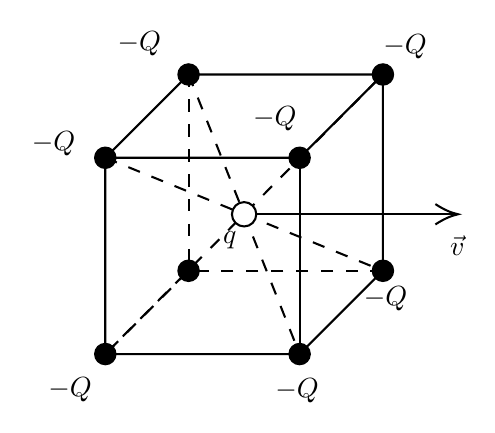
\begin{tikzpicture}[x=0.75pt,y=0.75pt,yscale=-1,xscale=1]
%uncomment if require: \path (0,205); %set diagram left start at 0, and has height of 205

%Shape: Cube [id:dp912316329494171] 
\draw   (281.41,73.63) -- (321.54,33.5) -- (415.17,33.5) -- (415.17,128.07) -- (375.05,168.2) -- (281.41,168.2) -- cycle ; \draw   (415.17,33.5) -- (375.05,73.63) -- (281.41,73.63) ; \draw   (375.05,73.63) -- (375.05,168.2) ;
%Straight Lines [id:da7932497906208718] 
\draw  [dash pattern={on 4.5pt off 4.5pt}]  (321.54,33.5) -- (321.54,128.07) ;
%Straight Lines [id:da2949920190066182] 
\draw  [dash pattern={on 4.5pt off 4.5pt}]  (415.17,128.07) -- (321.91,128.07) ;
%Straight Lines [id:da7606271813543024] 
\draw  [dash pattern={on 4.5pt off 4.5pt}]  (321.54,128.07) -- (281.41,168.2) ;
%Flowchart: Connector [id:dp31345639797296543] 
\draw  [fill={rgb, 255:red, 0; green, 0; blue, 0 }  ,fill opacity=1 ] (276.5,73.63) .. controls (276.5,70.92) and (278.7,68.72) .. (281.41,68.72) .. controls (284.13,68.72) and (286.33,70.92) .. (286.33,73.63) .. controls (286.33,76.35) and (284.13,78.55) .. (281.41,78.55) .. controls (278.7,78.55) and (276.5,76.35) .. (276.5,73.63) -- cycle ;
%Flowchart: Connector [id:dp4464434240009014] 
\draw  [fill={rgb, 255:red, 0; green, 0; blue, 0 }  ,fill opacity=1 ] (276.5,168.2) .. controls (276.5,165.48) and (278.7,163.28) .. (281.41,163.28) .. controls (284.13,163.28) and (286.33,165.48) .. (286.33,168.2) .. controls (286.33,170.91) and (284.13,173.11) .. (281.41,173.11) .. controls (278.7,173.11) and (276.5,170.91) .. (276.5,168.2) -- cycle ;
%Flowchart: Connector [id:dp5397376605990161] 
\draw  [fill={rgb, 255:red, 0; green, 0; blue, 0 }  ,fill opacity=1 ] (410.26,128.07) .. controls (410.26,125.36) and (412.46,123.15) .. (415.17,123.15) .. controls (417.89,123.15) and (420.09,125.36) .. (420.09,128.07) .. controls (420.09,130.79) and (417.89,132.99) .. (415.17,132.99) .. controls (412.46,132.99) and (410.26,130.79) .. (410.26,128.07) -- cycle ;
%Flowchart: Connector [id:dp5549760416410436] 
\draw  [fill={rgb, 255:red, 0; green, 0; blue, 0 }  ,fill opacity=1 ] (316.63,128.07) .. controls (316.63,125.36) and (318.83,123.15) .. (321.54,123.15) .. controls (324.26,123.15) and (326.46,125.36) .. (326.46,128.07) .. controls (326.46,130.79) and (324.26,132.99) .. (321.54,132.99) .. controls (318.83,132.99) and (316.63,130.79) .. (316.63,128.07) -- cycle ;
%Flowchart: Connector [id:dp4088669328872736] 
\draw  [fill={rgb, 255:red, 0; green, 0; blue, 0 }  ,fill opacity=1 ] (370.13,168.2) .. controls (370.13,165.48) and (372.33,163.28) .. (375.05,163.28) .. controls (377.76,163.28) and (379.96,165.48) .. (379.96,168.2) .. controls (379.96,170.91) and (377.76,173.11) .. (375.05,173.11) .. controls (372.33,173.11) and (370.13,170.91) .. (370.13,168.2) -- cycle ;
%Flowchart: Connector [id:dp64439132917289] 
\draw  [fill={rgb, 255:red, 0; green, 0; blue, 0 }  ,fill opacity=1 ] (410.26,33.5) .. controls (410.26,30.79) and (412.46,28.59) .. (415.17,28.59) .. controls (417.89,28.59) and (420.09,30.79) .. (420.09,33.5) .. controls (420.09,36.22) and (417.89,38.42) .. (415.17,38.42) .. controls (412.46,38.42) and (410.26,36.22) .. (410.26,33.5) -- cycle ;
%Flowchart: Connector [id:dp7347777412639311] 
\draw  [fill={rgb, 255:red, 0; green, 0; blue, 0 }  ,fill opacity=1 ] (316.63,33.5) .. controls (316.63,30.79) and (318.83,28.59) .. (321.54,28.59) .. controls (324.26,28.59) and (326.46,30.79) .. (326.46,33.5) .. controls (326.46,36.22) and (324.26,38.42) .. (321.54,38.42) .. controls (318.83,38.42) and (316.63,36.22) .. (316.63,33.5) -- cycle ;
%Straight Lines [id:da2803367819444311] 
\draw  [dash pattern={on 4.5pt off 4.5pt}]  (321.54,33.5) -- (375.05,168.2) ;
%Straight Lines [id:da35461993566128225] 
\draw  [dash pattern={on 4.5pt off 4.5pt}]  (281.41,168.2) -- (415.17,33.5) ;
%Straight Lines [id:da9428194669615855] 
\draw  [dash pattern={on 4.5pt off 4.5pt}]  (281.41,73.63) -- (415.17,128.07) ;
%Flowchart: Connector [id:dp4387373875976397] 
\draw  [fill={rgb, 255:red, 0; green, 0; blue, 0 }  ,fill opacity=1 ] (370.13,73.63) .. controls (370.13,70.92) and (372.33,68.72) .. (375.05,68.72) .. controls (377.76,68.72) and (379.96,70.92) .. (379.96,73.63) .. controls (379.96,76.35) and (377.76,78.55) .. (375.05,78.55) .. controls (372.33,78.55) and (370.13,76.35) .. (370.13,73.63) -- cycle ;
%Shape: Circle [id:dp14560268109648877] 
\draw  [fill={rgb, 255:red, 255; green, 255; blue, 255 }  ,fill opacity=1 ] (342.43,100.85) .. controls (342.43,97.61) and (345.06,94.99) .. (348.29,94.99) .. controls (351.53,94.99) and (354.16,97.61) .. (354.16,100.85) .. controls (354.16,104.09) and (351.53,106.72) .. (348.29,106.72) .. controls (345.06,106.72) and (342.43,104.09) .. (342.43,100.85) -- cycle ;
%Straight Lines [id:da4587184341973549] 
\draw    (354.16,100.85) -- (449.38,100.85) ;
\draw [shift={(451.38,100.85)}, rotate = 180] [color={rgb, 255:red, 0; green, 0; blue, 0 }  ][line width=0.75]    (10.93,-4.9) .. controls (6.95,-2.3) and (3.31,-0.67) .. (0,0) .. controls (3.31,0.67) and (6.95,2.3) .. (10.93,4.9)   ;



% Text Node
\draw (252.52,178.12) node [anchor=north west][inner sep=0.75pt]    {$-Q$};
% Text Node
\draw (244.52,59.45) node [anchor=north west][inner sep=0.75pt]    {$-Q$};
% Text Node
\draw (285.85,11.45) node [anchor=north west][inner sep=0.75pt]    {$-Q$};
% Text Node
\draw (413.85,12.79) node [anchor=north west][inner sep=0.75pt]    {$-Q$};
% Text Node
\draw (351.19,47.63) node [anchor=north west][inner sep=0.75pt]    {$-Q$};
% Text Node
\draw (404.52,134.3) node [anchor=north west][inner sep=0.75pt]    {$-Q$};
% Text Node
\draw (361.85,178.3) node [anchor=north west][inner sep=0.75pt]    {$-Q$};
% Text Node
\draw (336.67,107.73) node [anchor=north west][inner sep=0.75pt]    {$q$};
% Text Node
\draw (446,109.73) node [anchor=north west][inner sep=0.75pt]    {$\vec{v}$};


\end{tikzpicture}
 
    \end{minipage}
   \begin{minipage}{0.5\textwidth}
         Thế năng lúc hạt ở sát một mặt của hình lập phương (ngay lúc vừa ra khỏi hình lập phương):
    \begin{equation*}
    \begin{aligned}
         U_{f}&=-4 \dfrac{k q Q}{\dfrac{l}{\sqrt{2}}}-4 \dfrac{k q Q}{l \sqrt{\dfrac{3}{2}}}\\
        &=-\left(4 \sqrt{2}+4 \sqrt{\dfrac{2}{3}}\right) \dfrac{k q Q}{l}.
    \end{aligned}
    \end{equation*}
    \\
   \end{minipage}
   \begin{minipage}{0.5\textwidth}
         

\tikzset{every picture/.style={line width=0.75pt}} %set default line width to 0.75pt        

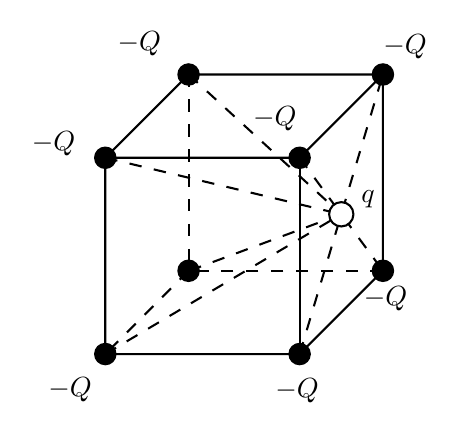
\begin{tikzpicture}[x=0.75pt,y=0.75pt,yscale=-1,xscale=1]
%uncomment if require: \path (0,205); %set diagram left start at 0, and has height of 205

%Shape: Cube [id:dp24209537695489214] 
\draw   (281.41,73.63) -- (321.54,33.5) -- (415.17,33.5) -- (415.17,128.07) -- (375.05,168.2) -- (281.41,168.2) -- cycle ; \draw   (415.17,33.5) -- (375.05,73.63) -- (281.41,73.63) ; \draw   (375.05,73.63) -- (375.05,168.2) ;
%Straight Lines [id:da6552145415795416] 
\draw  [dash pattern={on 4.5pt off 4.5pt}]  (321.54,33.5) -- (321.54,128.07) ;
%Straight Lines [id:da9574617665960996] 
\draw  [dash pattern={on 4.5pt off 4.5pt}]  (415.17,128.07) -- (321.91,128.07) ;
%Straight Lines [id:da06581595655266037] 
\draw  [dash pattern={on 4.5pt off 4.5pt}]  (321.54,128.07) -- (281.41,168.2) ;
%Flowchart: Connector [id:dp41511649615136736] 
\draw  [fill={rgb, 255:red, 0; green, 0; blue, 0 }  ,fill opacity=1 ] (276.5,73.63) .. controls (276.5,70.92) and (278.7,68.72) .. (281.41,68.72) .. controls (284.13,68.72) and (286.33,70.92) .. (286.33,73.63) .. controls (286.33,76.35) and (284.13,78.55) .. (281.41,78.55) .. controls (278.7,78.55) and (276.5,76.35) .. (276.5,73.63) -- cycle ;
%Flowchart: Connector [id:dp4876596956950916] 
\draw  [fill={rgb, 255:red, 0; green, 0; blue, 0 }  ,fill opacity=1 ] (276.5,168.2) .. controls (276.5,165.48) and (278.7,163.28) .. (281.41,163.28) .. controls (284.13,163.28) and (286.33,165.48) .. (286.33,168.2) .. controls (286.33,170.91) and (284.13,173.11) .. (281.41,173.11) .. controls (278.7,173.11) and (276.5,170.91) .. (276.5,168.2) -- cycle ;
%Flowchart: Connector [id:dp4578757750078104] 
\draw  [fill={rgb, 255:red, 0; green, 0; blue, 0 }  ,fill opacity=1 ] (410.26,128.07) .. controls (410.26,125.36) and (412.46,123.15) .. (415.17,123.15) .. controls (417.89,123.15) and (420.09,125.36) .. (420.09,128.07) .. controls (420.09,130.79) and (417.89,132.99) .. (415.17,132.99) .. controls (412.46,132.99) and (410.26,130.79) .. (410.26,128.07) -- cycle ;
%Flowchart: Connector [id:dp39812879825306147] 
\draw  [fill={rgb, 255:red, 0; green, 0; blue, 0 }  ,fill opacity=1 ] (316.63,128.07) .. controls (316.63,125.36) and (318.83,123.15) .. (321.54,123.15) .. controls (324.26,123.15) and (326.46,125.36) .. (326.46,128.07) .. controls (326.46,130.79) and (324.26,132.99) .. (321.54,132.99) .. controls (318.83,132.99) and (316.63,130.79) .. (316.63,128.07) -- cycle ;
%Flowchart: Connector [id:dp35502902150570725] 
\draw  [fill={rgb, 255:red, 0; green, 0; blue, 0 }  ,fill opacity=1 ] (370.13,168.2) .. controls (370.13,165.48) and (372.33,163.28) .. (375.05,163.28) .. controls (377.76,163.28) and (379.96,165.48) .. (379.96,168.2) .. controls (379.96,170.91) and (377.76,173.11) .. (375.05,173.11) .. controls (372.33,173.11) and (370.13,170.91) .. (370.13,168.2) -- cycle ;
%Flowchart: Connector [id:dp9259530091725627] 
\draw  [fill={rgb, 255:red, 0; green, 0; blue, 0 }  ,fill opacity=1 ] (410.26,33.5) .. controls (410.26,30.79) and (412.46,28.59) .. (415.17,28.59) .. controls (417.89,28.59) and (420.09,30.79) .. (420.09,33.5) .. controls (420.09,36.22) and (417.89,38.42) .. (415.17,38.42) .. controls (412.46,38.42) and (410.26,36.22) .. (410.26,33.5) -- cycle ;
%Flowchart: Connector [id:dp45876583578064944] 
\draw  [fill={rgb, 255:red, 0; green, 0; blue, 0 }  ,fill opacity=1 ] (316.63,33.5) .. controls (316.63,30.79) and (318.83,28.59) .. (321.54,28.59) .. controls (324.26,28.59) and (326.46,30.79) .. (326.46,33.5) .. controls (326.46,36.22) and (324.26,38.42) .. (321.54,38.42) .. controls (318.83,38.42) and (316.63,36.22) .. (316.63,33.5) -- cycle ;
%Straight Lines [id:da905955850885398] 
\draw  [dash pattern={on 4.5pt off 4.5pt}]  (321.54,33.5) -- (395.11,100.85) ;
%Straight Lines [id:da9670866838623073] 
\draw  [dash pattern={on 4.5pt off 4.5pt}]  (375.05,168.2) -- (415.17,33.5) ;
%Straight Lines [id:da7266251533013184] 
\draw  [dash pattern={on 4.5pt off 4.5pt}]  (375.05,73.63) -- (415.17,128.07) ;
%Flowchart: Connector [id:dp5253855939543575] 
\draw  [fill={rgb, 255:red, 0; green, 0; blue, 0 }  ,fill opacity=1 ] (370.13,73.63) .. controls (370.13,70.92) and (372.33,68.72) .. (375.05,68.72) .. controls (377.76,68.72) and (379.96,70.92) .. (379.96,73.63) .. controls (379.96,76.35) and (377.76,78.55) .. (375.05,78.55) .. controls (372.33,78.55) and (370.13,76.35) .. (370.13,73.63) -- cycle ;
%Straight Lines [id:da19896497025807758] 
\draw  [dash pattern={on 4.5pt off 4.5pt}]  (281.41,73.63) -- (395.11,100.85) ;
%Straight Lines [id:da878238857030275] 
\draw  [dash pattern={on 4.5pt off 4.5pt}]  (281.41,168.2) -- (395.11,100.85) ;
%Straight Lines [id:da7466399768898722] 
\draw  [dash pattern={on 4.5pt off 4.5pt}]  (321.91,128.07) -- (395.11,100.85) ;
%Shape: Circle [id:dp48972228222895464] 
\draw  [fill={rgb, 255:red, 255; green, 255; blue, 255 }  ,fill opacity=1 ] (389.25,100.85) .. controls (389.25,97.61) and (391.87,94.99) .. (395.11,94.99) .. controls (398.35,94.99) and (400.97,97.61) .. (400.97,100.85) .. controls (400.97,104.09) and (398.35,106.72) .. (395.11,106.72) .. controls (391.87,106.72) and (389.25,104.09) .. (389.25,100.85) -- cycle ;

% Text Node
\draw (252.52,178.12) node [anchor=north west][inner sep=0.75pt]    {$-Q$};
% Text Node
\draw (244.52,59.45) node [anchor=north west][inner sep=0.75pt]    {$-Q$};
% Text Node
\draw (285.85,11.45) node [anchor=north west][inner sep=0.75pt]    {$-Q$};
% Text Node
\draw (413.85,12.79) node [anchor=north west][inner sep=0.75pt]    {$-Q$};
% Text Node
\draw (351.19,47.63) node [anchor=north west][inner sep=0.75pt]    {$-Q$};
% Text Node
\draw (404.52,134.3) node [anchor=north west][inner sep=0.75pt]    {$-Q$};
% Text Node
\draw (361.85,178.3) node [anchor=north west][inner sep=0.75pt]    {$-Q$};
% Text Node
\draw (403.33,87.73) node [anchor=north west][inner sep=0.75pt]    {$q$};
\end{tikzpicture}
   \end{minipage}
    Bảo toàn năng lượng, ta có:
    \begin{equation*}
        \dfrac{mv^2}{2}+U_i=U_f+E \\
        \Leftrightarrow\dfrac{mv^2}{2}=\left(-4 \sqrt{2}-4 \sqrt{\dfrac{2}{3}}+\dfrac{16}{\sqrt{3}}\right) \dfrac{k q Q}{l}+E.
    \end{equation*}
    Từ đó tính được $v=0,354\dv{m/s^2}$.
    \end{loigiai}
    
    \begin{vd}[Điện dung của hệ hình trụ]
\begin{enumerate}[1)]
    \item Tìm điện dung của một đơn vị chiều dài giữa một cặp dây dẫn hình trụ song song có bán kính $R$ và cách nhau một khoảng $d(d\gg R)$, như trong hình $(a)$.
    \item Một dây dẫn hình trụ có bán kính $R$ được đặt ở trên một tấm dẫn phẳng được nối đất, cách mặt phẳng dẫn một đoạn $d(d\gg R)$, như hình $(b)$. Tìm điện dung của một đơn vị chiều dài giữa hai vật dẫn đó.
\end{enumerate}
\begin{center}


\tikzset{every picture/.style={line width=0.75pt}} %set default line width to 0.75pt        

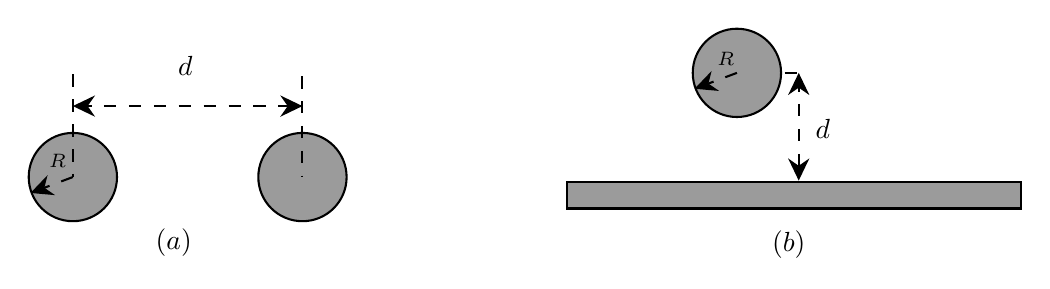
\begin{tikzpicture}[x=0.75pt,y=0.75pt,yscale=-1,xscale=1]
%uncomment if require: \path (0,300); %set diagram left start at 0, and has height of 300

%Straight Lines [id:da677113196713506] 
\draw  [dash pattern={on 4.5pt off 4.5pt}]  (68.27,136.47) -- (172.9,136.47) ;
\draw [shift={(175.9,136.47)}, rotate = 180] [fill={rgb, 255:red, 0; green, 0; blue, 0 }  ][line width=0.08]  [draw opacity=0] (10.72,-5.15) -- (0,0) -- (10.72,5.15) -- (7.12,0) -- cycle    ;
\draw [shift={(65.27,136.47)}, rotate = 0] [fill={rgb, 255:red, 0; green, 0; blue, 0 }  ][line width=0.08]  [draw opacity=0] (10.72,-5.15) -- (0,0) -- (10.72,5.15) -- (7.12,0) -- cycle    ;
%Shape: Circle [id:dp874210144956922] 
\draw  [fill={rgb, 255:red, 155; green, 155; blue, 155 }  ,fill opacity=1 ] (44,170.67) .. controls (44,158.92) and (53.52,149.4) .. (65.27,149.4) .. controls (77.02,149.4) and (86.54,158.92) .. (86.54,170.67) .. controls (86.54,182.42) and (77.02,191.94) .. (65.27,191.94) .. controls (53.52,191.94) and (44,182.42) .. (44,170.67) -- cycle ;
%Shape: Circle [id:dp1813413337643932] 
\draw  [fill={rgb, 255:red, 155; green, 155; blue, 155 }  ,fill opacity=1 ] (154.62,170.67) .. controls (154.62,158.92) and (164.14,149.4) .. (175.89,149.4) .. controls (187.64,149.4) and (197.16,158.92) .. (197.16,170.67) .. controls (197.16,182.42) and (187.64,191.94) .. (175.89,191.94) .. controls (164.14,191.94) and (154.62,182.42) .. (154.62,170.67) -- cycle ;
%Straight Lines [id:da5768044451421217] 
\draw  [dash pattern={on 4.5pt off 4.5pt}]  (175.89,122.03) -- (175.89,170.67) ;
%Straight Lines [id:da2702097859751069] 
\draw  [dash pattern={on 4.5pt off 4.5pt}]  (65.27,121.18) -- (65.27,170.67) ;
%Straight Lines [id:da6104556670247443] 
\draw  [dash pattern={on 4.5pt off 4.5pt}]  (65.27,170.67) -- (47.68,177.28) ;
\draw [shift={(44.87,178.33)}, rotate = 339.43] [fill={rgb, 255:red, 0; green, 0; blue, 0 }  ][line width=0.08]  [draw opacity=0] (10.72,-5.15) -- (0,0) -- (10.72,5.15) -- (7.12,0) -- cycle    ;
%Shape: Rectangle [id:dp6837421498436178] 
\draw  [fill={rgb, 255:red, 155; green, 155; blue, 155 }  ,fill opacity=1 ] (303.52,173.23) -- (522.22,173.23) -- (522.22,185.82) -- (303.52,185.82) -- cycle ;
%Shape: Circle [id:dp2448813293793357] 
\draw  [fill={rgb, 255:red, 155; green, 155; blue, 155 }  ,fill opacity=1 ] (363.93,120.47) .. controls (363.93,108.72) and (373.46,99.2) .. (385.21,99.2) .. controls (396.96,99.2) and (406.48,108.72) .. (406.48,120.47) .. controls (406.48,132.22) and (396.96,141.74) .. (385.21,141.74) .. controls (373.46,141.74) and (363.93,132.22) .. (363.93,120.47) -- cycle ;
%Straight Lines [id:da6679308714290266] 
\draw  [dash pattern={on 4.5pt off 4.5pt}]  (385.21,120.47) -- (367.61,127.07) ;
\draw [shift={(364.8,128.13)}, rotate = 339.43] [fill={rgb, 255:red, 0; green, 0; blue, 0 }  ][line width=0.08]  [draw opacity=0] (10.72,-5.15) -- (0,0) -- (10.72,5.15) -- (7.12,0) -- cycle    ;
%Straight Lines [id:da016736600541896518] 
\draw  [dash pattern={on 4.5pt off 4.5pt}]  (414.99,123.47) -- (414.99,169.37) ;
\draw [shift={(414.99,172.37)}, rotate = 270] [fill={rgb, 255:red, 0; green, 0; blue, 0 }  ][line width=0.08]  [draw opacity=0] (10.72,-5.15) -- (0,0) -- (10.72,5.15) -- (7.12,0) -- cycle    ;
\draw [shift={(414.99,120.47)}, rotate = 90] [fill={rgb, 255:red, 0; green, 0; blue, 0 }  ][line width=0.08]  [draw opacity=0] (10.72,-5.15) -- (0,0) -- (10.72,5.15) -- (7.12,0) -- cycle    ;
%Straight Lines [id:da049016635462894476] 
\draw  [dash pattern={on 4.5pt off 4.5pt}]  (408.17,120.47) -- (414.99,120.47) ;

% Text Node
\draw (52.39,158.1) node [anchor=north west][inner sep=0.75pt]  [font=\scriptsize]  {$R$};
% Text Node
\draw (103.7,194.31) node [anchor=north west][inner sep=0.75pt]    {$( a)$};
% Text Node
\draw (374.33,108.89) node [anchor=north west][inner sep=0.75pt]  [font=\scriptsize]  {$R$};
% Text Node
\draw (114.51,110.93) node [anchor=north west][inner sep=0.75pt]    {$d$};
% Text Node
\draw (421.68,141.56) node [anchor=north west][inner sep=0.75pt]    {$d$};
% Text Node
\draw (400.66,195.16) node [anchor=north west][inner sep=0.75pt]    {$( b)$};


\end{tikzpicture}
\end{center}
\end{vd}
\begin{loigiai}
\begin{enumerate}[1)]
    \item Giả sử một sợi dây cáp có mật độ điện dài $\lambda$ và dây còn lại có mật độ điện dài $-\lambda$.\\
    Chọn đường nối hai tâm dây cáp làm trục $X$ và chọn $x=0$ tại trung điểm giữa hai dây cáp.\\
    Điện trường toàn phần tại một điểm trên trục $X$ là:
    \[E=\dfrac{\lambda}{2\pi\varepsilon_0}\left(\dfrac{1}{\dfrac{d}{2}+x}+\dfrac{1}{\dfrac{d}{2}-x}\right).\]
    Hiệu điện thế giữa hai dây cáp:
    \begin{align*}
    U&=\int_{-(\dfrac{d}{2}-R)}^{\dfrac{d}{2}-R}E\mathrm{d}x=\dfrac{\lambda}{2\pi\varepsilon_0}\left.\left[\ln{\left(\dfrac{d}{2}+x\right)}-\ln{\left(\dfrac{d}{2}-x\right)}\right]\right|_{-\left(\dfrac{d}{2}-R\right)}^{\left(\dfrac{d}{2}-R\right)}\\
    &=\dfrac{\lambda}{\pi\varepsilon_0}\ln{\left(\dfrac{d-R}{R}\right)}\approx \dfrac{\lambda}{\pi\varepsilon_0}\ln{\left(\dfrac{d}{R}\right)}.
    \end{align*}
    Điện dung của hệ $2$ dây cáp là:
    \[C=\dfrac{Q}{U}=\dfrac{\pi\varepsilon_0}{\ln{\left(\dfrac{2d}{R}\right)}}.\]
    \item Áp dụng phương pháp ảnh điện, điện trường là:
    \[E=\dfrac{\lambda}{2\pi\varepsilon_0}\left(\dfrac{1}{d+x}+\dfrac{1}{d-x}\right).\]
    Hiệu điện thế là:
    \begin{align*}
        U&=\int_{-(d-R)}^{0}E\mathrm{d}x=\dfrac{\lambda}{2\pi\varepsilon_0}\left.\left[\ln{(d+x)-\ln{(d-x)}}\right]\right|_{-(d-R)}^{0}\\
        &=\dfrac{\lambda}{2\pi\varepsilon_0}\ln{\left(\dfrac{2d-R}{R}\right)}\approx \dfrac{\lambda}{2\pi\varepsilon_0}\ln{\left(\dfrac{2d}{R}\right)}.
        \end{align*}
        Điện dung của hệ:
        \[C=\dfrac{Q}{U}=\dfrac{2\pi\varepsilon_0}{\ln{\left(\dfrac{2d}{R}\right)}}.\]
\end{enumerate}
\end{loigiai}

    \begin{vd}[Mô hình phân cực]
    \begin{minipage}{0.65\textwidth}
      Chúng ta coi rằng một quả cầu trung hòa về điện là sự kết hợp của hai quả cầu khác nhau: một quả cầu tích điện đều theo thể tích với mật độ $+\rho$, bao gồm các hạt nhân của các nguyên tử, quả còn lại có cùng bán kính tích điện đều với mật độ $-\rho$, bao gồm các electron. Giả sử rằng bằng một cách nào đó chúng ta có thể dịch chuyển hai quả cầu này sao cho tâm của chúng cách nhau một khoảng $\delta$ như trong hình, mà không làm thay đổi cầu trúc của hai quả cầu.\\
    Tìm điện trường tạo bởi phân bố điện tích trên:
    \end{minipage}
    \begin{minipage}{0.3\textwidth}
      \centering

\tikzset{every picture/.style={line width=0.75pt}} %set default line width to 0.75pt        

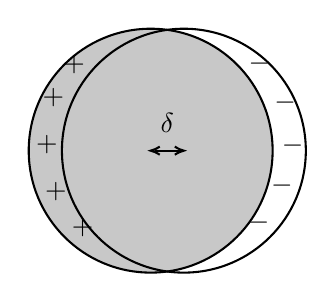
\begin{tikzpicture}[x=0.75pt,y=0.75pt,yscale=-1,xscale=1]
%uncomment if require: \path (0,179); %set diagram left start at 0, and has height of 179

%Shape: Circle [id:dp348067281994352] 
\draw  [fill={rgb, 255:red, 200; green, 200; blue, 200 }  ,fill opacity=1 ] (245.33,91.25) .. controls (245.33,58.81) and (271.64,32.5) .. (304.09,32.5) .. controls (336.53,32.5) and (362.84,58.81) .. (362.84,91.25) .. controls (362.84,123.7) and (336.53,150.01) .. (304.09,150.01) .. controls (271.64,150.01) and (245.33,123.7) .. (245.33,91.25) -- cycle ;
%Shape: Circle [id:dp010283630354624318] 
\draw   (261.33,91.25) .. controls (261.33,58.81) and (287.64,32.5) .. (320.09,32.5) .. controls (352.53,32.5) and (378.84,58.81) .. (378.84,91.25) .. controls (378.84,123.7) and (352.53,150.01) .. (320.09,150.01) .. controls (287.64,150.01) and (261.33,123.7) .. (261.33,91.25) -- cycle ;
%Straight Lines [id:da7330655663361718] 
\draw    (306.09,91.25) -- (318.09,91.25) ;
\draw [shift={(320.09,91.25)}, rotate = 180] [color={rgb, 255:red, 0; green, 0; blue, 0 }  ][line width=0.75]    (4.37,-1.96) .. controls (2.78,-0.92) and (1.32,-0.27) .. (0,0) .. controls (1.32,0.27) and (2.78,0.92) .. (4.37,1.96)   ;
\draw [shift={(304.09,91.25)}, rotate = 0] [color={rgb, 255:red, 0; green, 0; blue, 0 }  ][line width=0.75]    (4.37,-1.96) .. controls (2.78,-0.92) and (1.32,-0.27) .. (0,0) .. controls (1.32,0.27) and (2.78,0.92) .. (4.37,1.96)   ;

% Text Node
\draw (260.59,43.94) node [anchor=north west][inner sep=0.75pt]    {$+$};
% Text Node
\draw (250.59,59.58) node [anchor=north west][inner sep=0.75pt]    {$+$};
% Text Node
\draw (247.39,82.38) node [anchor=north west][inner sep=0.75pt]    {$+$};
% Text Node
\draw (251.79,105.18) node [anchor=north west][inner sep=0.75pt]    {$+$};
% Text Node
\draw (264.59,122.38) node [anchor=north west][inner sep=0.75pt]    {$+$};
% Text Node
\draw (349.39,120.17) node [anchor=north west][inner sep=0.75pt]    {$-$};
% Text Node
\draw (360.59,101.98) node [anchor=north west][inner sep=0.75pt]    {$-$};
% Text Node
\draw (365.79,82.78) node [anchor=north west][inner sep=0.75pt]    {$-$};
% Text Node
\draw (362.19,61.98) node [anchor=north west][inner sep=0.75pt]    {$-$};
% Text Node
\draw (349.79,43.58) node [anchor=north west][inner sep=0.75pt]    {$-$};
% Text Node
\draw (307.39,71.75) node [anchor=north west][inner sep=0.75pt]    {$\delta $};


\end{tikzpicture}

    \end{minipage}
    \begin{enumerate}[1)]
    \setlength{\itemsep}{0pt}
        \item Tại vùng không gian giao nhau giữa hai quả cầu.
        \item Tại vùng không gian bên ngoài hai quả cầu, đánh giá kết quả khi $\delta\ll R$.
    \end{enumerate}
    \end{vd}
    \begin{loigiai}
    \begin{enumerate}[1)]
        \item Theo nguyên lý chồng chất, điện trường tại một điểm trong không gian sẽ là sự tổng hợp điện trường sinh ra bởi hai quả cầu.\\
        Đối với một quả cầu riêng biệt tích điện với mật độ điện khối $\rho$, điện trường do quả cầu tạo ra tại một điểm cách tâm nó một khoảng $r<R$ là:
        \begin{equation*}
            \ot{E}=\dfrac{4\pi k\rho \ot{r}}{3}.
        \end{equation*}
        Coi rằng tâm của hai quả cầu nằm trên trục $x$ và tâm của hai quả cầu có tọa độ lần lượt là $O_+\tron{\dfrac{\delta}{2},0,0}$ và $O_-\tron{-\dfrac{\delta}{2},0,0}$.
        \begin{center}
            

\tikzset{every picture/.style={line width=0.75pt}} %set default line width to 0.75pt        

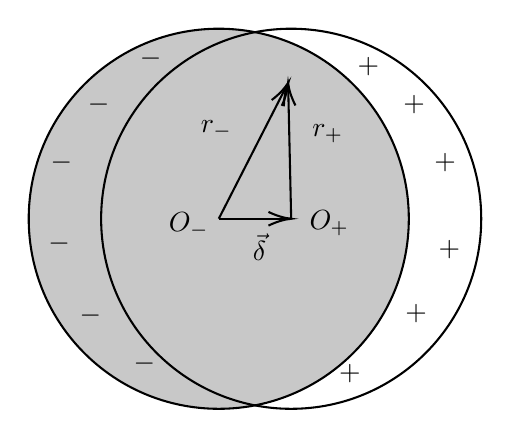
\begin{tikzpicture}[x=0.75pt,y=0.75pt,yscale=-1,xscale=1]
%uncomment if require: \path (0,221); %set diagram left start at 0, and has height of 221

%Shape: Circle [id:dp017437485907043415] 
\draw  [color={rgb, 255:red, 0; green, 0; blue, 0 }  ,draw opacity=1 ][fill={rgb, 255:red, 200; green, 200; blue, 200 }  ,fill opacity=1 ] (226,108.56) .. controls (226,57.99) and (266.99,17) .. (317.56,17) .. controls (368.13,17) and (409.13,57.99) .. (409.13,108.56) .. controls (409.13,159.13) and (368.13,200.13) .. (317.56,200.13) .. controls (266.99,200.13) and (226,159.13) .. (226,108.56) -- cycle ;
%Shape: Circle [id:dp8644229876539793] 
\draw   (260.89,108.56) .. controls (260.89,57.99) and (301.89,17) .. (352.45,17) .. controls (403.02,17) and (444.02,57.99) .. (444.02,108.56) .. controls (444.02,159.13) and (403.02,200.13) .. (352.45,200.13) .. controls (301.89,200.13) and (260.89,159.13) .. (260.89,108.56) -- cycle ;
%Straight Lines [id:da3225302970061237] 
\draw    (317.56,108.56) -- (350.45,108.56) ;
\draw [shift={(352.45,108.56)}, rotate = 180] [color={rgb, 255:red, 0; green, 0; blue, 0 }  ][line width=0.75]    (10.93,-3.29) .. controls (6.95,-1.4) and (3.31,-0.3) .. (0,0) .. controls (3.31,0.3) and (6.95,1.4) .. (10.93,3.29)   ;
%Straight Lines [id:da03191807652795409] 
\draw    (317.56,108.56) -- (350.06,44.91) ;
\draw [shift={(350.97,43.13)}, rotate = 477.05] [color={rgb, 255:red, 0; green, 0; blue, 0 }  ][line width=0.75]    (10.93,-3.29) .. controls (6.95,-1.4) and (3.31,-0.3) .. (0,0) .. controls (3.31,0.3) and (6.95,1.4) .. (10.93,3.29)   ;
%Straight Lines [id:da4064808818545982] 
\draw    (352.45,108.56) -- (351.02,45.13) ;
\draw [shift={(350.97,43.13)}, rotate = 448.7] [color={rgb, 255:red, 0; green, 0; blue, 0 }  ][line width=0.75]    (10.93,-3.29) .. controls (6.95,-1.4) and (3.31,-0.3) .. (0,0) .. controls (3.31,0.3) and (6.95,1.4) .. (10.93,3.29)   ;

% Text Node
\draw (359.85,103.27) node [anchor=north west][inner sep=0.75pt]    {$O_{+}$};
% Text Node
\draw (292.05,104.24) node [anchor=north west][inner sep=0.75pt]    {$O_{-}$};
% Text Node
\draw (361.13,61.45) node [anchor=north west][inner sep=0.75pt]    {$\ot{r_{+}}$};
% Text Node
\draw (307.46,59.68) node [anchor=north west][inner sep=0.75pt]    {$\ot{r_{-}}$};
% Text Node
\draw (332.49,114.2) node [anchor=north west][inner sep=0.75pt]    {$\vec{\delta }$};
% Text Node
\draw (374,177.4) node [anchor=north west][inner sep=0.75pt]    {$+$};
% Text Node
\draw (406,148.4) node [anchor=north west][inner sep=0.75pt]    {$+$};
% Text Node
\draw (383,29.4) node [anchor=north west][inner sep=0.75pt]    {$+$};
% Text Node
\draw (420,75.4) node [anchor=north west][inner sep=0.75pt]    {$+$};
% Text Node
\draw (405,47.4) node [anchor=north west][inner sep=0.75pt]    {$+$};
% Text Node
\draw (422,117.38) node [anchor=north west][inner sep=0.75pt]    {$+$};
% Text Node
\draw (253,47.4) node [anchor=north west][inner sep=0.75pt]    {$-$};
% Text Node
\draw (235,75.4) node [anchor=north west][inner sep=0.75pt]    {$-$};
% Text Node
\draw (234,114.4) node [anchor=north west][inner sep=0.75pt]    {$-$};
% Text Node
\draw (249,149.4) node [anchor=north west][inner sep=0.75pt]    {$-$};
% Text Node
\draw (275,172.38) node [anchor=north west][inner sep=0.75pt]    {$-$};
% Text Node
\draw (278,25.38) node [anchor=north west][inner sep=0.75pt]    {$-$};


\end{tikzpicture}

        \end{center}
        Ta có:
        \begin{equation*}
            \begin{aligned}
                 &\ot{r_+}=\ot{r}+\dfrac{\ot{\delta}}{2},\\
                 &\ot{r_-}=\ot{r}-\dfrac{\ot{\delta}}{2}.
            \end{aligned}
        \end{equation*}
        Điện trường tại vùng giao nhau của hai quả cầu:
        \begin{equation*}
            \ot{E}=\dfrac{4\pi k\rho \tron{\ot{r}-\dfrac{\ot{\delta}}{2}}}{3}-\dfrac{4\pi k\rho\tron{\ot{r}+\dfrac{\ot{\delta}}{2}}}{3}=-\dfrac{4\pi k\rho\ot{\delta}}{3}.
        \end{equation*}
       \item Điện trường do một quả cầu bán kính $R$, tích điện đều với mật độ điện khối $\rho$ gây ra ở vùng không gian bên ngoài quả cầu giống như điện trường của một điện tích điểm $Q=\dfrac{4\pi R^3 \rho}{3}$ đặt tại tâm quả cầu. Vậy nên, điện trường do hai quả cầu gây ra tại vùng không gian bên ngoài quả cầu giống như điện trường gây ra bởi hai điện tích điểm $\pm Q$ đặt tại $O_+$ và $O_-$. Nếu $R\gg \delta$, điện trường này tương đương với điện trường của một lưỡng cực điện có moment lưỡng cực:
        $$\ot{p}=Q\ot{\delta}=\dfrac{4\pi R^3\rho}{3}\ot{\delta} . $$
        Điện trường tạo ra:
        $$\ot{E}=k\tron{\dfrac{\ot{r}\tron{\ot{p}\cdot\ot{r}}}{r^5}-\dfrac{\ot{p}}{r^3}}.$$
    \end{enumerate}
    \end{loigiai}
    
    
    
    \begin{vd}[Điện trường trong hốc cầu rỗng]
    \begin{minipage}{0.5\textwidth}
      Một quả cầu đồng chất bán kính $a$ tích điện đều với mật độ điện tích $\rho$. Người ta khoét ở bên trong quả cầu một khoang trống hình cầu bán kính $b<a$, bên trong khoang không tích điện. Tâm của khoang $O_b$ cách tâm của hình cầu $O_a$ một khoảng $d$, với $d<(a-b)$.
    \end{minipage}
    \begin{minipage}{0.5\textwidth}
      \centering
\tikzset{every picture/.style={line width=0.75pt}} %set default line width to 0.75pt        

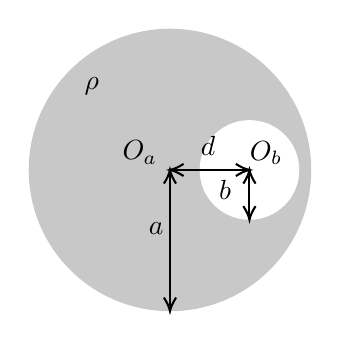
\begin{tikzpicture}[x=0.75pt,y=0.75pt,yscale=-1,xscale=1]
%uncomment if require: \path (0,179); %set diagram left start at 0, and has height of 179

%Shape: Circle [id:dp5133875522475451] 
\draw  [color={rgb, 255:red, 0; green, 0; blue, 0 }  ,draw opacity=0 ][fill={rgb, 255:red, 200; green, 200; blue, 200 }  ,fill opacity=1 ] (282.33,94.05) .. controls (282.33,56.47) and (312.8,26) .. (350.39,26) .. controls (387.97,26) and (418.44,56.47) .. (418.44,94.05) .. controls (418.44,131.64) and (387.97,162.1) .. (350.39,162.1) .. controls (312.8,162.1) and (282.33,131.64) .. (282.33,94.05) -- cycle ;
%Shape: Ellipse [id:dp5662859497643196] 
\draw  [color={rgb, 255:red, 0; green, 0; blue, 0 }  ,draw opacity=0 ][fill={rgb, 255:red, 255; green, 255; blue, 255 }  ,fill opacity=1 ] (364.67,94.05) .. controls (364.67,80.79) and (375.42,70.04) .. (388.68,70.04) .. controls (401.94,70.04) and (412.69,80.79) .. (412.69,94.05) .. controls (412.69,107.31) and (401.94,118.06) .. (388.68,118.06) .. controls (375.42,118.06) and (364.67,107.31) .. (364.67,94.05) -- cycle ;
%Straight Lines [id:da523226980810126] 
\draw    (350.39,96.05) -- (350.39,160.1) ;
\draw [shift={(350.39,162.1)}, rotate = 270] [color={rgb, 255:red, 0; green, 0; blue, 0 }  ][line width=0.75]    (6.56,-2.94) .. controls (4.17,-1.38) and (1.99,-0.4) .. (0,0) .. controls (1.99,0.4) and (4.17,1.38) .. (6.56,2.94)   ;
\draw [shift={(350.39,94.05)}, rotate = 90] [color={rgb, 255:red, 0; green, 0; blue, 0 }  ][line width=0.75]    (6.56,-2.94) .. controls (4.17,-1.38) and (1.99,-0.4) .. (0,0) .. controls (1.99,0.4) and (4.17,1.38) .. (6.56,2.94)   ;
%Straight Lines [id:da7784251747453967] 
\draw    (388.68,96.05) -- (388.68,116.06) ;
\draw [shift={(388.68,118.06)}, rotate = 270] [color={rgb, 255:red, 0; green, 0; blue, 0 }  ][line width=0.75]    (6.56,-2.94) .. controls (4.17,-1.38) and (1.99,-0.4) .. (0,0) .. controls (1.99,0.4) and (4.17,1.38) .. (6.56,2.94)   ;
\draw [shift={(388.68,94.05)}, rotate = 90] [color={rgb, 255:red, 0; green, 0; blue, 0 }  ][line width=0.75]    (6.56,-2.94) .. controls (4.17,-1.38) and (1.99,-0.4) .. (0,0) .. controls (1.99,0.4) and (4.17,1.38) .. (6.56,2.94)   ;
%Straight Lines [id:da2698365651836454] 
\draw    (352.39,94.05) -- (386.68,94.05) ;
\draw [shift={(388.68,94.05)}, rotate = 180] [color={rgb, 255:red, 0; green, 0; blue, 0 }  ][line width=0.75]    (6.56,-2.94) .. controls (4.17,-1.38) and (1.99,-0.4) .. (0,0) .. controls (1.99,0.4) and (4.17,1.38) .. (6.56,2.94)   ;
\draw [shift={(350.39,94.05)}, rotate = 0] [color={rgb, 255:red, 0; green, 0; blue, 0 }  ][line width=0.75]    (6.56,-2.94) .. controls (4.17,-1.38) and (1.99,-0.4) .. (0,0) .. controls (1.99,0.4) and (4.17,1.38) .. (6.56,2.94)   ;

% Text Node
\draw (363.73,76.11) node [anchor=north west][inner sep=0.75pt]    {$d$};
% Text Node
\draw (372.53,97.45) node [anchor=north west][inner sep=0.75pt]    {$b$};
% Text Node
\draw (387.44,78.95) node [anchor=north west][inner sep=0.75pt]    {$O_{b}$};
% Text Node
\draw (338.69,117.95) node [anchor=north west][inner sep=0.75pt]    {$a$};
% Text Node
\draw (326.05,78.61) node [anchor=north west][inner sep=0.75pt]    {$O_{a}$};
% Text Node
\draw (307.82,47.98) node [anchor=north west][inner sep=0.75pt]    {$\rho $};
\end{tikzpicture}
    \end{minipage}
    \begin{enumerate}[1)]
        \setlength{\itemsep}{0pt}
        \item Tìm điện trường tại vùng không gian bên trong khoang trống.\\
        \end{enumerate}
         Bây giờ toàn bộ quả cầu được đặt trong điện trường đều có cường độ điện trường $E_0$.
        \begin{enumerate}[1)]
        \setcounter{enumi}{1}
        \item Tìm lực tác dụng lên quả cầu.
        \item Tìm moment lực tác dụng lên quả cầu đối với quả cầu và đối với khối tâm quả cầu.
    \end{enumerate}
    \end{vd}
    \begin{loigiai}
    \begin{enumerate}[1)]
    \setlength{\itemsep}{0pt}
        \item Một quả cầu có mật độ điện tích $\rho$ với một khoang trống hình cầu không điện tích có thể coi như là một quả cầu tích điện $\rho$ khắp thể tích của nó và một quả cầu khác tích điện $-\rho$. Điện trường tại một điểm trong không gian là tổng hợp của điện trường gây ra bởi hai quả cầu.
        \begin{center}
\tikzset{every picture/.style={line width=0.75pt}} %set default line width to 0.75pt        
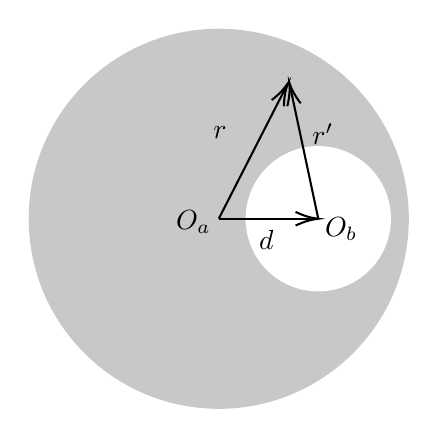
\begin{tikzpicture}[x=0.75pt,y=0.75pt,yscale=-1,xscale=1]
%uncomment if require: \path (0,221); %set diagram left start at 0, and has height of 221

%Shape: Circle [id:dp017437485907043415] 
\draw  [color={rgb, 255:red, 255; green, 255; blue, 255 }  ,draw opacity=0 ][fill={rgb, 255:red, 200; green, 200; blue, 200 }  ,fill opacity=1 ] (226,108.56) .. controls (226,57.99) and (266.99,17) .. (317.56,17) .. controls (368.13,17) and (409.13,57.99) .. (409.13,108.56) .. controls (409.13,159.13) and (368.13,200.13) .. (317.56,200.13) .. controls (266.99,200.13) and (226,159.13) .. (226,108.56) -- cycle ;
%Flowchart: Connector [id:dp8574035111298091] 
\draw  [color={rgb, 255:red, 0; green, 0; blue, 0 }  ,draw opacity=0 ][fill={rgb, 255:red, 255; green, 255; blue, 255 }  ,fill opacity=1 ] (330.51,108.56) .. controls (330.51,89.23) and (346.18,73.56) .. (365.51,73.56) .. controls (384.84,73.56) and (400.51,89.23) .. (400.51,108.56) .. controls (400.51,127.89) and (384.84,143.56) .. (365.51,143.56) .. controls (346.18,143.56) and (330.51,127.89) .. (330.51,108.56) -- cycle ;
%Straight Lines [id:da3225302970061237] 
\draw    (317.56,108.56) -- (363.51,108.56) ;
\draw [shift={(365.51,108.56)}, rotate = 180] [color={rgb, 255:red, 0; green, 0; blue, 0 }  ][line width=0.75]    (10.93,-3.29) .. controls (6.95,-1.4) and (3.31,-0.3) .. (0,0) .. controls (3.31,0.3) and (6.95,1.4) .. (10.93,3.29)   ;
%Straight Lines [id:da03191807652795409] 
\draw    (317.56,108.56) -- (350.06,44.91) ;
\draw [shift={(350.97,43.13)}, rotate = 477.05] [color={rgb, 255:red, 0; green, 0; blue, 0 }  ][line width=0.75]    (10.93,-3.29) .. controls (6.95,-1.4) and (3.31,-0.3) .. (0,0) .. controls (3.31,0.3) and (6.95,1.4) .. (10.93,3.29)   ;
%Straight Lines [id:da4064808818545982] 
\draw    (365.51,108.56) -- (351.96,44.91) ;
\draw [shift={(351.54,42.95)}, rotate = 437.98] [color={rgb, 255:red, 0; green, 0; blue, 0 }  ][line width=0.75]    (10.93,-3.29) .. controls (6.95,-1.4) and (3.31,-0.3) .. (0,0) .. controls (3.31,0.3) and (6.95,1.4) .. (10.93,3.29)   ;

% Text Node
\draw (367.28,106.35) node [anchor=north west][inner sep=0.75pt]    {$O_{b}$};
% Text Node
\draw (295.55,103.24) node [anchor=north west][inner sep=0.75pt]    {$O_{a}$};
% Text Node
\draw (361.13,61.45) node [anchor=north west][inner sep=0.75pt]    {$\ot{r'}$};
% Text Node
\draw (313.46,62.68) node [anchor=north west][inner sep=0.75pt]    {$\ot{r}$};
% Text Node
\draw (335.49,112.7) node [anchor=north west][inner sep=0.75pt]    {$\ot{d}$};


\end{tikzpicture}

        \end{center}
        Ta có:
        \begin{equation*}
            \ot{E}=\dfrac{4\pi k}{3}\tron{\ot{r}-\ot{r'}}=\dfrac{4\pi k}{3}\ot{d}.
        \end{equation*}
        Điện trường bên trong khoang trống là đều và song song với đường thằng nối tâm quả cầu và khoang trống.
        \item Khi hệ được đặt trong điện trường đều. Có thể coi lực tác dụng lên hệ như là lực mà điện trường tác dụng lên hai điện tích $q_a=\dfrac{4\pi a^3\rho}{3}$ và $q_b=-\dfrac{4\pi b^3\rho}{3}$ lần lượt đặt tại $O_a$ và $O_b$. \\ 
        Ta có:
        \begin{equation*}
            \ot{F}=\dfrac{4\pi k\tron{a^3-b^3}\rho}{3}\ot{E_0}.
        \end{equation*}
        \item Bởi vì hợp lực tác dụng lên hệ khác không nên moment lực tác dụng lên hệ phụ thuộc vào vị trí chọn tâm quay.\\
        Moment lực tác dụng lên quả cầu đối với tâm quay là $O_a$ là:
        $$\ot{T_1}=-\dfrac{4\pi b^3\rho}{4}\ot{d}\times\ot{E_0}.$$
        Ta chọn một hệ quy chiếu mới với trục $x$ đi qua $O_a$ và $O_b$, gốc tọa độ trùng với $O_a$. Gọi khối lượng riêng của quả cầu là $\rho_m$. Khối lượng của hệ là $M_c=\dfrac{4\pi \tron{a^3-b^3}\rho_m}{3}$. Tọa độ khối tâm của hệ là $x_c$. 
        \\
        Giả sử một quả cầu bán kính $b$ khối lượng $M_b=\dfrac{4\pi b^3\rho_m}{3}$ đặt tại khoang trống của quả cầu. Cả hệ bây giờ như một hình cầu đặc bán kính $a$, khối lượng $M_a=\dfrac{4\pi a^3\rho_m}{3}$ đặt tại $O_a$ có tọa độ bằng không. Ta có:
        $$0=\dfrac{M_cx_c+M_bd}{M_a}\Leftrightarrow x_c=-d\dfrac{M_b}{M_c}=-d\dfrac{b^3}{a^3-b^3}.$$
        Moment lực đối với khối tâm:
        $$\ot{T_2}=\tron{\dfrac{4\pi a^3\rho}{3}\tron{d\dfrac{b^3}{a^3-b^3}}-\dfrac{4\pi b^3\rho }{3}\tron{d+d\dfrac{b^3}{a^3-b^3}}}\tron{\ot{e_x}\times\ot{E_0}}=0.$$
        Trong đó $\ot{e_x}$ là vector đơn vị dọc theo trục $x$.\\
        Kết quả hợp lý vì khi đặt hệ trong điện trường đều, các phần tử của hệ đều chịu một lực tỉ lệ với thể tích, giống như đặt trong một trọng trường đều.
    \end{enumerate}
    \end{loigiai}
    
    
    \begin{vd}[Điện tích trên vòng]
Một hạt coi là chất điểm có khối lượng $m$ và điện tích $q$ chuyển động tự do không ma sát dọc theo một đường tròn nằm ngang cố định bán kính r. Trong mặt phẳng của vòng, một điện tích $Q$ khác được đặt ở một vị trí cố định, cách tâm vòng một khoảng $d$, với $d<r$ (xem hình vẽ). 
\begin{center}
    

\tikzset{every picture/.style={line width=0.75pt}} %set default line width to 0.75pt        

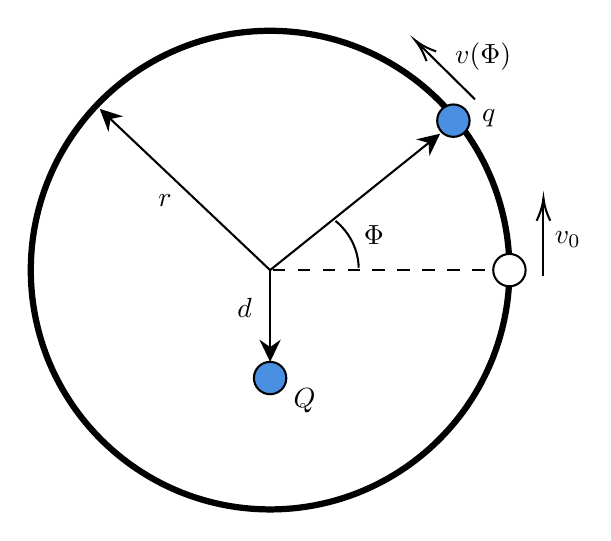
\begin{tikzpicture}[x=0.75pt,y=0.75pt,yscale=-1,xscale=1]
%uncomment if require: \path (0,470); %set diagram left start at 0, and has height of 470

%Shape: Circle [id:dp4352794293041511] 
\draw  [line width=2.25]  (201,179.3) .. controls (201,115.62) and (252.62,64) .. (316.3,64) .. controls (379.98,64) and (431.6,115.62) .. (431.6,179.3) .. controls (431.6,242.98) and (379.98,294.6) .. (316.3,294.6) .. controls (252.62,294.6) and (201,242.98) .. (201,179.3) -- cycle ;
%Straight Lines [id:da5040476830588836] 
\draw  [dash pattern={on 4.5pt off 4.5pt}]  (431.6,179.3) -- (316.3,179.3) ;
%Shape: Circle [id:dp3864705024915467] 
\draw  [fill={rgb, 255:red, 255; green, 255; blue, 255 }  ,fill opacity=1 ] (423.8,179.3) .. controls (423.8,174.99) and (427.29,171.5) .. (431.6,171.5) .. controls (435.91,171.5) and (439.4,174.99) .. (439.4,179.3) .. controls (439.4,183.61) and (435.91,187.1) .. (431.6,187.1) .. controls (427.29,187.1) and (423.8,183.61) .. (423.8,179.3) -- cycle ;
%Shape: Circle [id:dp3760399239302583] 
\draw  [fill={rgb, 255:red, 74; green, 144; blue, 226 }  ,fill opacity=1 ] (396.8,107.3) .. controls (396.8,102.99) and (400.29,99.5) .. (404.6,99.5) .. controls (408.91,99.5) and (412.4,102.99) .. (412.4,107.3) .. controls (412.4,111.61) and (408.91,115.1) .. (404.6,115.1) .. controls (400.29,115.1) and (396.8,111.61) .. (396.8,107.3) -- cycle ;
%Straight Lines [id:da8336614182940776] 
\draw    (236.38,103.66) -- (316.3,179.3) ;
\draw [shift={(234.2,101.6)}, rotate = 43.42] [fill={rgb, 255:red, 0; green, 0; blue, 0 }  ][line width=0.08]  [draw opacity=0] (10.72,-5.15) -- (0,0) -- (10.72,5.15) -- (7.12,0) -- cycle    ;
%Straight Lines [id:da3530703705263947] 
\draw    (395.86,115.48) -- (316.3,179.3) ;
\draw [shift={(398.2,113.6)}, rotate = 141.26] [fill={rgb, 255:red, 0; green, 0; blue, 0 }  ][line width=0.08]  [draw opacity=0] (10.72,-5.15) -- (0,0) -- (10.72,5.15) -- (7.12,0) -- cycle    ;
%Shape: Circle [id:dp513558393549516] 
\draw  [fill={rgb, 255:red, 74; green, 144; blue, 226 }  ,fill opacity=1 ] (308.5,231.3) .. controls (308.5,226.99) and (311.99,223.5) .. (316.3,223.5) .. controls (320.61,223.5) and (324.1,226.99) .. (324.1,231.3) .. controls (324.1,235.61) and (320.61,239.1) .. (316.3,239.1) .. controls (311.99,239.1) and (308.5,235.61) .. (308.5,231.3) -- cycle ;
%Straight Lines [id:da050747851797288135] 
\draw    (316.3,179.3) -- (316.3,220.5) ;
\draw [shift={(316.3,223.5)}, rotate = 270] [fill={rgb, 255:red, 0; green, 0; blue, 0 }  ][line width=0.08]  [draw opacity=0] (10.72,-5.15) -- (0,0) -- (10.72,5.15) -- (7.12,0) -- cycle    ;
%Shape: Arc [id:dp5089728896438459] 
\draw  [draw opacity=0] (347.8,155.61) .. controls (349.43,156.92) and (350.94,158.42) .. (352.31,160.11) .. controls (356.63,165.44) and (358.82,171.81) .. (358.99,178.17) -- (329,179) -- cycle ; \draw   (347.8,155.61) .. controls (349.43,156.92) and (350.94,158.42) .. (352.31,160.11) .. controls (356.63,165.44) and (358.82,171.81) .. (358.99,178.17) ;
%Straight Lines [id:da492782704805941] 
\draw    (415,97) -- (387.62,70) ;
\draw [shift={(386.2,68.6)}, rotate = 404.6] [color={rgb, 255:red, 0; green, 0; blue, 0 }  ][line width=0.75]    (10.93,-3.29) .. controls (6.95,-1.4) and (3.31,-0.3) .. (0,0) .. controls (3.31,0.3) and (6.95,1.4) .. (10.93,3.29)   ;
%Straight Lines [id:da7335237598222573] 
\draw    (448,182) -- (448,146.6) ;
\draw [shift={(448,144.6)}, rotate = 450] [color={rgb, 255:red, 0; green, 0; blue, 0 }  ][line width=0.75]    (10.93,-3.29) .. controls (6.95,-1.4) and (3.31,-0.3) .. (0,0) .. controls (3.31,0.3) and (6.95,1.4) .. (10.93,3.29)   ;


% Text Node
\draw (261,141.4) node [anchor=north west][inner sep=0.75pt]    {$r$};
% Text Node
\draw (299,191.4) node [anchor=north west][inner sep=0.75pt]    {$d$};
% Text Node
\draw (326.1,234.7) node [anchor=north west][inner sep=0.75pt]    {$Q$};
% Text Node
\draw (417,100.4) node [anchor=north west][inner sep=0.75pt]    {$q$};
% Text Node
\draw (360,156.4) node [anchor=north west][inner sep=0.75pt]    {$\Phi $};
% Text Node
\draw (404,68.4) node [anchor=north west][inner sep=0.75pt]    {$v( \Phi )$};
% Text Node
\draw (452,159.4) node [anchor=north west][inner sep=0.75pt]    {$v_{0}$};


\end{tikzpicture}
\end{center}
\begin{enumerate}[1)]
    \item Hạt nằm trên vòng có vận tốc ban đầu $v_0$. Tính vận tốc $v$ của nó dưới dạng một hàm của góc $\Phi$, $v(\Phi)$.
    \item Biểu diễn lực mà vòng tác dụng lên hạt dưới dạng một hàm của $\Phi$.
    \item Lực ma sát nhớt tác dụng lên hạt có hướng ngược lại với vận tốc, và độ lớn tỉ lệ với tốc độ: $\left| {{F_f}} \right| = m\gamma v$, trong đó $\gamma$ là hệ số tỉ lệ. Với $v_0$ là vận tốc ban đầu, hãy xác định vị trí mà hạt dừng lại.
\end{enumerate}
\end{vd}
\begin{loigiai}
\begin{enumerate}[1)]
    \item Áp dụng định luật bảo toàn năng lượng ta có:
    $$v^2+\dfrac{C}{\left| {\ot r - \ot {r_Q}} \right|}=const.$$
    với $C=\dfrac{Qq}{2\pi m \varepsilon_0}$.
    \\Từ hình vẽ, ta có: $\Phi(0)=0,~\Phi(Q)=-\pi/2$, và ta được:
    $$v(\Phi)^2=v_0^2+\dfrac{C}{\sqrt{r^2+d^2}}-\dfrac{C}{\sqrt{r^2+d^2+2rd\sin{\Phi}}}$$
    Vậy
    $$v(\Phi)=\sqrt{v_0^2+\dfrac{C}{\sqrt{r^2+d^2}}-\dfrac{C}{\sqrt{r^2+d^2+2rd\sin{\Phi}}}}$$
    \item Lực $F_n$ mà vòng tác dụng lên hạt là lực liên kết, pháp tuyến đối với vòng và hợp với các lực khác để tạo ra một tổng lực mà theo phương pháp tuyến bằng lực hướng tâm: $F_{ht}=m\dfrac{v^2}{R}$, hướng vào trong. Lực còn lại là lực đẩy Coulomb (nếu C>0) từ Q, với độ lớn:
    $$F_Q=\dfrac{mC}{2(r^2+d^2+2rd\sin{\Phi})}$$
    Thành phần pháp tuyến của nó có hệ số $\cos{\alpha}$, với $\alpha$ là góc giữa vector bán kính nối tâm với $q$ và đường thẳng $Qq$. Định lý cosin trên tam giác 3 đỉnh $q,Q$ và tâm vòng tròn:
    $$\cos{\alpha}=\dfrac{r+d\sin{\Phi}}{\sqrt{r^2+d^2+2rd\sin{\Phi}}}$$
    Ta tìm được:
    $$F_n=\dfrac{mv^2}{R}+\dfrac{mC(r+d\sin{\Phi})}{2({r^2+d^2+2rd\sin{\Phi}})^{3/2}}$$
    \item Khi hạt đứng yên, lực ma sát tiếp tuyến với vành đai tự động bằng không, và các lực khác phải cân bằng. Tất cả các lực pháp tuyến được tự động cân bằng bởi vòng thông qua lực liên kết. Chúng ta cần xem xét lực theo phương tiếp tuyến, lực này chỉ có thể đến từ lực Coulomb tác dụng lên $q$, và do đó thành phần tiếp tuyến của nó phải biến mất. Điều này chỉ có thể xảy ra ở hai nơi, tại điểm cực đại và cực tiểu tính từ $Q$, tức là ở điểm trên cùng hoặc dưới cùng.
    \end{enumerate}
\end{loigiai}
    \begin{vd}[Xuyên qua nhau]
    Hai quả cầu điện môi đặc có cùng bán kính $R$ và khối lượng $M$ nhưng được tích điện trái dấu $\pm Q$. Các điện tích phân bố đều trên cả hai quả cầu. Lúc đầu cả hai quả cầu đều đứng yên, tâm của hai quả cầu cách nhau một khoảng $x_0\gg R$, sao cho năng lượng tương tác giữa hai quả cầu là không đáng kể so với năng lượng tương tác giữa các điện tích trên cùng một quả cầu.
    \begin{enumerate}[1)]
    \setlength{\itemsep}{0pt}
        \item Tìm năng lượng lúc đầu của hệ.\\
        Sau khi bắt đầu, các quả cầu hút nhau do có điện tích trái dấu và dịch chuyển lại gần nhau.
        \item Tìm vận tốc của hai quả cầu sau khi hai quả cầu bắt đầu chạm vào nhau.
        \item Giả sử rằng, sau khi chạm vào nhau, các quả cầu bắt đầu chuyển động đâm xuyên qua nhau mà không chịu lực cản. Tìm vận tốc các quả cầu khi tâm của hai quả cầu trùng với nhau.
    \end{enumerate}
    \end{vd}
    \begin{loigiai}
    \begin{enumerate}[1)]
    \setlength{\itemsep}{0pt}
        \item Thế năng tĩnh điện của một quả cầu bán kính $R$ tích điện đều $Q$, theo như đã tính ở bài \ref{c291}, là
        $$U_0=\dfrac{3kQ^2}{5R}.$$
        Vậy nên năng lượng lúc đầu của hệ hai quả cầu là
        $$U_{\mathrm{tot}}=2U_0=\dfrac{6kQ^2}{5R}.$$
        \item Kí hiệu $x$ là khoảng cách giữa tâm của hai quả cầu. Khi $x$ đủ nhỏ để năng lượng tương tác giữa hai quả cầu $U_{\mathrm{tt}}(x)$ không còn được coi là không đáng kể so với năng lượng tương tác trong một quả cầu $U_0$ nữa, thì năng lượng của hệ là
        $$U_{\mathrm{tot}}=2U_0+U_{\mathrm{tt}}(x).$$
        Khi $x\geq 2R$ thì lực hút do hai quả cầu tác dụng lên nhau giống hệt như lực do hai điện tích điểm tác dụng lên nhau.\\
        Ta có
        $$U_{\mathrm{tt}}(x)=-\dfrac{kQ^2}{x}.$$
        Do động lượng của hệ bảo toàn, vận tốc của hai quả cầu luôn có độ lớn bằng nhau và ngược chiều nhau. \\
        Khi $x\geq 2R$, theo định luật bảo toàn năng lượng
        \begin{equation*}
        \begin{aligned}
           Mv^2+2U_0+U_{\mathrm{tt}}(x)=2U_0
           &\Leftrightarrow Mv^2+U_{\mathrm{tt}}(x)=0\\
           &\Leftrightarrow  v^2=\dfrac{kQ^2}{xM}.
        \end{aligned}
        \end{equation*}
        Khi hai quả cầu bắt đầu chạm vào nhau $x=2R$, khi đó vận tốc hai quả cầu là
        $$v=\sqrt{\dfrac{kQ^2}{2RM}}.$$
        \item Khi tâm của hai quả cầu trùng nhau, điện trường do hai quả cầu tạo ra triệt tiêu nhau tại mọi điểm trong không gian. Vậy nên, thế năng tương tác tĩnh điện bằng không. Toàn bộ thế năng tĩnh điện đã được chuyển thành động năng.\\
        Ta có
        \begin{equation*}
            \begin{aligned}
               Mv^2=2U_0\Leftrightarrow v=\sqrt{\dfrac{6kQ^2}{5RM}}.
            \end{aligned}
        \end{equation*}
    \end{enumerate}
    \end{loigiai}
    
     \begin{vd}[Dao động lệch tâm]
    Một quả cầu dẫn điện bán kính $a$ ban đầu trung hòa về điện. Quả cầu chứa $N$ electron dẫn. Một phần $f$ ($0<f<1$) các electron dẫn đột ngột thoát ra khỏi quả cầu, $(1-f)N$ các electron dẫn còn lại phân bố lại trong quả cầu đến khi đạt đến cân bằng tĩnh điện, trong khi đó các ion tại các nút mạng không di chuyển.
    \begin{enumerate}[1)]
    \setlength{\itemsep}{0pt}
        \item Tìm phân bố của các electron dẫn trong quả cầu và bán kính của phân bố đó.\\
         Bây giờ quả cầu các electron dẫn được dịch chuyển khỏi vị trí cân bằng một khoảng $\delta$ mà không thay đổi hình dạng cũng như phân bố electron, với $\delta$ đủ nhỏ để cho quả cầu electron vẫn nằm trong quả cầu ban đầu.
        \item Tìm điện trường bên trong quả cầu electron.
        \item Tìm tần số dao động của quả cầu electron khi đột ngột ``thả'' quả cầu electron. Coi rằng hình dạng của quả cầu và phân bố điện tích của quả cầu electron không đổi trong khi chuyển động.
    \end{enumerate}
    \end{vd}
     \begin{loigiai}
        \begin{enumerate}[1)]
        \setlength{\itemsep}{0pt}
            \item \hfill\\
            \begin{minipage}{0.5\textwidth}
            Khi đạt đến trạng thái cân bằng, số electron còn lại phải không chịu tác dụng của điện trường. Do tính đối xứng, các electron phân bố trong một hình cầu bán kính $b<a$ đồng tâm với lại quả cầu.\\
                Để điện trường bên trong hình cầu bằng không, mật độ điện tích bên trong hình cầu bằng không. Từ đó suy ra mật độ electron dẫn bên trong hình cầu bằng mật độ các ion dương tại các nút mạng trong hình cầu, $n_e=n_i$.
            \end{minipage}
            \begin{minipage}{0.5\textwidth}
                \centering

\tikzset{every picture/.style={line width=0.75pt}} %set default line width to 0.75pt        

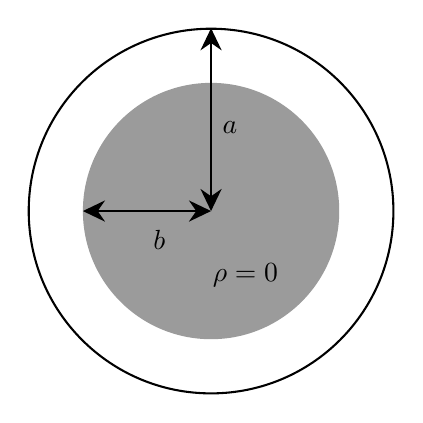
\begin{tikzpicture}[x=0.75pt,y=0.75pt,yscale=-1,xscale=1]
%uncomment if require: \path (0,181); %set diagram left start at 0, and has height of 181

%Shape: Circle [id:dp37132252659089415] 
\draw   (263,89.9) .. controls (263,41.38) and (302.33,2.05) .. (350.85,2.05) .. controls (399.37,2.05) and (438.71,41.38) .. (438.71,89.9) .. controls (438.71,138.42) and (399.37,177.75) .. (350.85,177.75) .. controls (302.33,177.75) and (263,138.42) .. (263,89.9) -- cycle ;
%Shape: Circle [id:dp7326766079222706] 
\draw  [color={rgb, 255:red, 0; green, 0; blue, 0 }  ,draw opacity=0 ][fill={rgb, 255:red, 155; green, 155; blue, 155 }  ,fill opacity=1 ] (289.1,89.9) .. controls (289.1,55.79) and (316.75,28.14) .. (350.85,28.14) .. controls (384.96,28.14) and (412.61,55.79) .. (412.61,89.9) .. controls (412.61,124.01) and (384.96,151.65) .. (350.85,151.65) .. controls (316.75,151.65) and (289.1,124.01) .. (289.1,89.9) -- cycle ;
%Straight Lines [id:da6815798853192978] 
\draw    (350.85,86.9) -- (350.85,4.81) ;
\draw [shift={(350.85,1.81)}, rotate = 450] [fill={rgb, 255:red, 0; green, 0; blue, 0 }  ][line width=0.08]  [draw opacity=0] (10.72,-5.15) -- (0,0) -- (10.72,5.15) -- (7.12,0) -- cycle    ;
\draw [shift={(350.85,89.9)}, rotate = 270] [fill={rgb, 255:red, 0; green, 0; blue, 0 }  ][line width=0.08]  [draw opacity=0] (10.72,-5.15) -- (0,0) -- (10.72,5.15) -- (7.12,0) -- cycle    ;
%Straight Lines [id:da6916068788534726] 
\draw    (292.1,89.9) -- (347.85,89.9) ;
\draw [shift={(350.85,89.9)}, rotate = 180] [fill={rgb, 255:red, 0; green, 0; blue, 0 }  ][line width=0.08]  [draw opacity=0] (10.72,-5.15) -- (0,0) -- (10.72,5.15) -- (7.12,0) -- cycle    ;
\draw [shift={(289.1,89.9)}, rotate = 0] [fill={rgb, 255:red, 0; green, 0; blue, 0 }  ][line width=0.08]  [draw opacity=0] (10.72,-5.15) -- (0,0) -- (10.72,5.15) -- (7.12,0) -- cycle    ;

% Text Node
\draw (321.6,97.48) node [anchor=north west][inner sep=0.75pt]    {$b$};
% Text Node
\draw (354.89,45.4) node [anchor=north west][inner sep=0.75pt]    {$a$};
% Text Node
\draw (350.23,113.88) node [anchor=north west][inner sep=0.75pt]    {$\rho =0$};


\end{tikzpicture}

            \end{minipage}
            Ta có 
            $$n_i=\dfrac{3N}{4\pi a^3} \ \text{và} \  n_e=\dfrac{3(1-f)N}{4 \pi b^3}.$$
            Suy ra 
            $$b=a\sqrt[3]{1-f}.$$
            \item \hfill \\
            \begin{minipage}{0.5\textwidth}
                 Bây giờ tâm "quả cầu" electron $O'$ được dịch chuyển một đoạn $\delta$ so với tâm quả cầu kim loại $O$ mà không thay đổi hình dạng cũng như mật độ điện tích như trên hình. Sử dụng nguyên lý chồng chất điện trường, điện trường bên trong quả cầu electron là tổng hợp của điện trường sinh ra bởi các electron trong quả cầu và điện trường sinh ra bởi các ion ở các nút mạng. Điện trường $\ot{E_P}$ tại điểm $P$ bên trong quả cầu electron:
            $$\ot{E_P}=\dfrac{4\pi k}{3}\dfrac{3Ne}{4\pi a^3}\tron{\ot{r}-\ot{r'}}=\frac{kNe}{a^3}\ot{\delta}.$$
            Điện trường bên trong quả cầu elctron là đều và có hướng cùng hướng với độ dịch chuyển $\ot{\delta}$.
            \end{minipage}
            \begin{minipage}{0.5\textwidth}
                \centering
                

\tikzset{every picture/.style={line width=0.75pt}} %set default line width to 0.75pt        

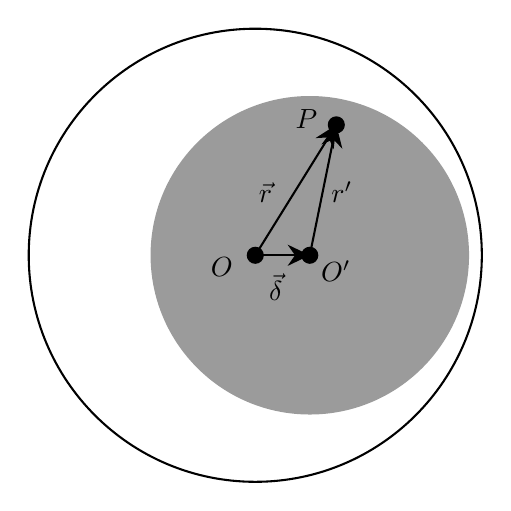
\begin{tikzpicture}[x=0.75pt,y=0.75pt,yscale=-1,xscale=1]
%uncomment if require: \path (0,287); %set diagram left start at 0, and has height of 287

%Shape: Ellipse [id:dp37132252659089415] 
\draw   (233,136.2) .. controls (233,75.92) and (281.87,27.05) .. (342.15,27.05) .. controls (402.44,27.05) and (451.31,75.92) .. (451.31,136.2) .. controls (451.31,196.48) and (402.44,245.35) .. (342.15,245.35) .. controls (281.87,245.35) and (233,196.48) .. (233,136.2) -- cycle ;
%Shape: Ellipse [id:dp7326766079222706] 
\draw  [color={rgb, 255:red, 0; green, 0; blue, 0 }  ,draw opacity=0 ][fill={rgb, 255:red, 155; green, 155; blue, 155 }  ,fill opacity=1 ] (291.7,136.2) .. controls (291.7,93.82) and (326.05,59.47) .. (368.42,59.47) .. controls (410.8,59.47) and (445.15,93.82) .. (445.15,136.2) .. controls (445.15,178.57) and (410.8,212.93) .. (368.42,212.93) .. controls (326.05,212.93) and (291.7,178.57) .. (291.7,136.2) -- cycle ;
%Shape: Ellipse [id:dp8134292801767902] 
\draw  [fill={rgb, 255:red, 0; green, 0; blue, 0 }  ,fill opacity=1 ] (364.81,136.2) .. controls (364.81,134.21) and (366.43,132.59) .. (368.42,132.59) .. controls (370.42,132.59) and (372.03,134.21) .. (372.03,136.2) .. controls (372.03,138.19) and (370.42,139.81) .. (368.42,139.81) .. controls (366.43,139.81) and (364.81,138.19) .. (364.81,136.2) -- cycle ;
%Shape: Circle [id:dp6145176668402599] 
\draw  [fill={rgb, 255:red, 0; green, 0; blue, 0 }  ,fill opacity=1 ] (338.54,136.2) .. controls (338.54,134.21) and (340.16,132.59) .. (342.15,132.59) .. controls (344.15,132.59) and (345.76,134.21) .. (345.76,136.2) .. controls (345.76,138.19) and (344.15,139.81) .. (342.15,139.81) .. controls (340.16,139.81) and (338.54,138.19) .. (338.54,136.2) -- cycle ;
%Straight Lines [id:da3473639118873846] 
\draw    (342.15,136.2) -- (365.42,136.2) ;
\draw [shift={(368.42,136.2)}, rotate = 540] [fill={rgb, 255:red, 0; green, 0; blue, 0 }  ][line width=0.08]  [draw opacity=0] (10.72,-5.15) -- (0,0) -- (10.72,5.15) -- (7.12,0) -- cycle    ;
%Shape: Ellipse [id:dp8471164676347949] 
\draw  [fill={rgb, 255:red, 0; green, 0; blue, 0 }  ,fill opacity=1 ] (377.59,73.37) .. controls (377.59,71.37) and (379.21,69.76) .. (381.2,69.76) .. controls (383.2,69.76) and (384.81,71.37) .. (384.81,73.37) .. controls (384.81,75.36) and (383.2,76.98) .. (381.2,76.98) .. controls (379.21,76.98) and (377.59,75.36) .. (377.59,73.37) -- cycle ;
%Straight Lines [id:da3258970291335339] 
\draw    (342.15,136.2) -- (379.62,75.91) ;
\draw [shift={(381.2,73.37)}, rotate = 481.86] [fill={rgb, 255:red, 0; green, 0; blue, 0 }  ][line width=0.08]  [draw opacity=0] (10.72,-5.15) -- (0,0) -- (10.72,5.15) -- (7.12,0) -- cycle    ;
%Straight Lines [id:da3602631306397466] 
\draw    (368.42,136.2) -- (380.6,76.31) ;
\draw [shift={(381.2,73.37)}, rotate = 461.5] [fill={rgb, 255:red, 0; green, 0; blue, 0 }  ][line width=0.08]  [draw opacity=0] (10.72,-5.15) -- (0,0) -- (10.72,5.15) -- (7.12,0) -- cycle    ;

% Text Node
\draw (319.3,135.77) node [anchor=north west][inner sep=0.75pt]    {$O$};
% Text Node
\draw (372.33,137.11) node [anchor=north west][inner sep=0.75pt]    {$O'$};
% Text Node
\draw (347.37,143.58) node [anchor=north west][inner sep=0.75pt]    {$\vec{\delta }$};
% Text Node
\draw (342.37,99.58) node [anchor=north west][inner sep=0.75pt]    {$\vec{r}$};
% Text Node
\draw (377.37,99.25) node [anchor=north west][inner sep=0.75pt]    {$\ot{r'}$};
% Text Node
\draw (360.04,64.73) node [anchor=north west][inner sep=0.75pt]    {$P$};


\end{tikzpicture}

            \end{minipage}
            \item Mỗi electron phải chịu một lực là
            $$\ot{F_P}=e\ot{E_P}=-\dfrac{kNe^2}{a^3}\ot{\delta}.$$
            Lực này tỉ lệ với $\delta$. Tổng lực tác dụng lên quả cầu electron là
            $$\ot{F}=-\dfrac{kN^2e^2}{a^3}\ot{\delta}.$$
            Ta có
            \begin{equation*}
                \begin{aligned}
                   Nm_e\dfrac{\dd^2\delta}{\dd t^2}=\dfrac{kN^2e^2}{a^3}\delta
                   \Leftrightarrow& ~\omega^2=\dfrac{kNe^2}{a^3m_e},\\
                   \Leftrightarrow&~\omega=\sqrt{\dfrac{kNe^2}{a^3m_e}}.
                \end{aligned}
            \end{equation*}
        \end{enumerate}
    \end{loigiai}
    
    
\begin{vd}[Điện thế hệ vỏ cầu]
Hai mặt cầu bán kính $r$ và $R$ $(r<R)$ lồng vào nhau đồng tâm. Ở bên trong mặt cầu nhỏ hơn được chứa đầy điện tích với mật độ điện tích trên một đơn vị thể tích là $-\rho$, khoảng không gian giữa hai mặt cầu chứa đầy điện tích với mật độ điện tích khối là $+\rho$ và không có điện tích ở bên ngoài bề mặt quả cầu lớn hơn. Tìm tỉ số $R/r$ để điện thế tại tâm của hệ bằng điện thế ở vô cùng.
\begin{center}
    

% Gradient Info
  
\tikzset {_fq8w470ev/.code = {\pgfsetadditionalshadetransform{ \pgftransformshift{\pgfpoint{0 bp } { 0 bp }  }  \pgftransformscale{1.5 }  }}}
\pgfdeclareradialshading{_38irhn25h}{\pgfpoint{0bp}{0bp}}{rgb(0bp)=(1,1,1);
rgb(0.8928571428571428bp)=(1,1,1);
rgb(25bp)=(0,0,0);
rgb(400bp)=(0,0,0)}
\tikzset{every picture/.style={line width=0.75pt}} %set default line width to 0.75pt        

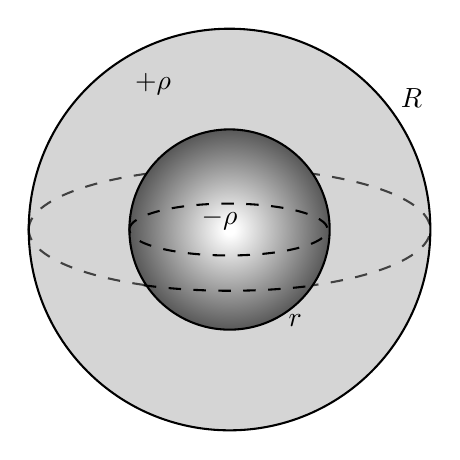
\begin{tikzpicture}[x=0.75pt,y=0.75pt,yscale=-1,xscale=1]
%uncomment if require: \path (0,452); %set diagram left start at 0, and has height of 452

%Shape: Ellipse [id:dp9929177085843359] 
\draw  [dash pattern={on 4.5pt off 4.5pt}] (165.25,159) .. controls (165.25,142.71) and (208.57,129.5) .. (262,129.5) .. controls (315.43,129.5) and (358.75,142.71) .. (358.75,159) .. controls (358.75,175.29) and (315.43,188.5) .. (262,188.5) .. controls (208.57,188.5) and (165.25,175.29) .. (165.25,159) -- cycle ;
%Shape: Circle [id:dp5348546769453121] 
\draw  [fill={rgb, 255:red, 155; green, 155; blue, 155 }  ,fill opacity=0.42 ] (165.25,159) .. controls (165.25,105.57) and (208.57,62.25) .. (262,62.25) .. controls (315.43,62.25) and (358.75,105.57) .. (358.75,159) .. controls (358.75,212.43) and (315.43,255.75) .. (262,255.75) .. controls (208.57,255.75) and (165.25,212.43) .. (165.25,159) -- cycle ;
%Shape: Circle [id:dp009094968300005002] 
\path  [shading=_38irhn25h,_fq8w470ev] (213.75,159) .. controls (213.75,132.35) and (235.35,110.75) .. (262,110.75) .. controls (288.65,110.75) and (310.25,132.35) .. (310.25,159) .. controls (310.25,185.65) and (288.65,207.25) .. (262,207.25) .. controls (235.35,207.25) and (213.75,185.65) .. (213.75,159) -- cycle ; % for fading 
 \draw  [line width=0.75]  (213.75,159) .. controls (213.75,132.35) and (235.35,110.75) .. (262,110.75) .. controls (288.65,110.75) and (310.25,132.35) .. (310.25,159) .. controls (310.25,185.65) and (288.65,207.25) .. (262,207.25) .. controls (235.35,207.25) and (213.75,185.65) .. (213.75,159) -- cycle ; % for border 

%Shape: Ellipse [id:dp562289767970725] 
\draw  [dash pattern={on 4.5pt off 4.5pt}] (213.75,159) .. controls (213.75,152.1) and (235.13,146.5) .. (261.5,146.5) .. controls (287.87,146.5) and (309.25,152.1) .. (309.25,159) .. controls (309.25,165.9) and (287.87,171.5) .. (261.5,171.5) .. controls (235.13,171.5) and (213.75,165.9) .. (213.75,159) -- cycle ;
%Shape: Arc [id:dp4771619674622566] 
\draw  [draw opacity=0][dash pattern={on 4.5pt off 4.5pt}] (298.53,186.46) .. controls (287.21,187.78) and (274.89,188.5) .. (262,188.5) .. controls (245.92,188.5) and (230.73,187.38) .. (217.28,185.38) -- (262,159) -- cycle ; \draw  [dash pattern={on 4.5pt off 4.5pt}] (298.53,186.46) .. controls (287.21,187.78) and (274.89,188.5) .. (262,188.5) .. controls (245.92,188.5) and (230.73,187.38) .. (217.28,185.38) ;

% Text Node
\draw (247,147.4) node [anchor=north west][inner sep=0.75pt]    {$-\rho $};
% Text Node
\draw (215,82.4) node [anchor=north west][inner sep=0.75pt]    {$+\rho $};
% Text Node
\draw (343,89.4) node [anchor=north west][inner sep=0.75pt]    {$R$};
% Text Node
\draw (289,198.4) node [anchor=north west][inner sep=0.75pt]    {$r$};


\end{tikzpicture}
\end{center}
\end{vd}
\begin{loigiai}
Theo tính đối xứng, hiệu điện thế giữa tâm của một khối cầu tích điện đều với điện thế ở vô cùng bằng:
\[\varphi \sim k \dfrac{q}{R} \sim \alpha \dfrac{\rho R^{3}}{R} \sim \alpha \rho R^{2}, \tag{1}\]
trong đó $\alpha$ biểu diễn một hệ số tỉ lệ giống nhau đối với một hình cầu có kích thước bất kỳ.\\
Hệ của chúng ta bây giờ có thể coi bao gồm một hình cầu có bán kính $R$ tích điện với mật độ khối $\rho$ chồng chất với một hình cầu bán kính $r$ tích điện với mật độ khối $-2\rho$, khi đó ta được:
\[\alpha \rho R^{2}+\alpha(-2 \rho) r^{2}=0. \tag{2}\]
Và ta thu được câu trả lời:
\[\dfrac{R}{r}=\sqrt{2}. \tag{3}\]
\end{loigiai}


\begin{vd}[Một bài toán có tiềm năng$^1$]
\footnotetext{$^1$Tên gốc của bài toán là ``A problem with potential''. Ở đấy tác giả đã có ý chơi chữ, ``potential'' vừa có nghĩa là tiềm năng vừa có nghĩa là điện thế. Bạn hiểu chứ?}
   Lego lấy hai chiếc vỏ làm từ vật liệu dẫn điện hình bán cầu có cùng bán kính và ghép chúng lại với nhau sao cho hai chiếc vỏ không tiếp xúc điện với nhau và chúng tạo thành một hình cầu. Sau đó anh ấy tích điện cho một bán cầu đến điện thế $U_1=100\dv{V}$ và bán cầu còn lại đến điện thế $U_2=-100\dv{V}$. Tìm điện thế tại tâm của hình cầu. 
    \end{vd}
    \begin{loigiai}
       Chúng ta có thể giải bài toán bằng cách giải phương trình Laplace. Tuy nhiên, chúng ta sẽ không giải theo hướng này. Thay vào đó, kí hiệu $\varphi$ là điện thế tại tâm quả cầu. Nếu chúng ta thay $U_1=-100\dv{V}$ và $U_2=100\dv{V}$, tức là đổi dấu điện thế hai nửa quả cầu, thì mọi đại lượng khác trong bài toán cũng sẽ đổi dấu, và điện thế tại tâm quả cầu lúc này là $-\varphi$. Nhưng việc đổi dấu điện thế hai nửa quả cầu cũng giống như là việc quay quả cầu $180^\circ$, việc này không làm ảnh hưởng đến điện thế tại tâm quả cầu. Vậy nên, điện thế tại tâm quả cầu lúc này vẫn phải là $\varphi$. Từ đó ta có:
        \[\varphi=-\varphi.\]
        Phương trình trên chỉ có một nghiệm, đó là $\varphi=0\dv{V}$. Vậy điện thế tại tâm quả cầu là $\varphi=0\dv{V}$.
    \end{loigiai}
    
    
    \begin{vd}[Tụ điện Cantor]
    Một hình trụ dài đồng chất được làm từ một vật liệu dẫn điện. Đầu tiên chúng ta chia trụ thành ba phần bằng nhau rồi bỏ phần ở giữa đi. Sau đó, chúng ta lại tiếp tục làm như vậy với hai hình trụ còn lại. Tiếp tục làm như vậy đến khi còn $2048$ hình trụ. \\
    Sau đó ta nối hai hình trụ ngoài cùng với một nguồn điện một chiều không đổi và đo được điện dung của hệ lúc này là $C_1$. Nếu ta tiếp tục chia các hình trụ thành ba phần rồi bỏ phần giữa đi thì giá trị điện dung của hệ tiến đến một giá trị $C_0$. 
    Coi như bán kính của hình trụ là rất lớn so với khoảng cách giữa hai hình trụ bất kì nào.\\
    Hãy tìm $\displaystyle\dfrac{C_1}{C_0}$.
     \begin{center}
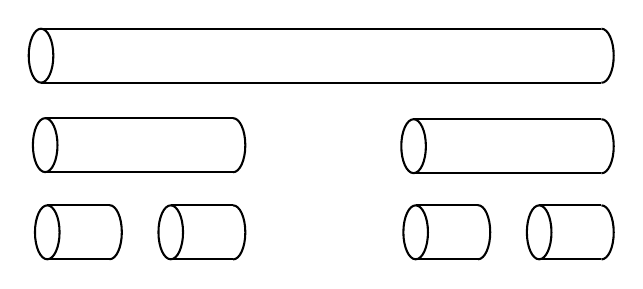
\begin{tikzpicture}[x=0.75pt,y=0.75pt,yscale=-1,xscale=1]
%uncomment if require: \path (0,155); %set diagram left start at 0, and has height of 155

%Straight Lines [id:da8779348118982053] 
\draw [fill={rgb, 255:red, 0; green, 0; blue, 0 }  ,fill opacity=0 ]   (216.66,29.01) -- (486.66,29.01) ;
%Straight Lines [id:da13466989557571818] 
\draw [fill={rgb, 255:red, 0; green, 0; blue, 0 }  ,fill opacity=0 ]   (216.66,55) -- (486.66,55) ;
%Shape: Ellipse [id:dp9259404166148435] 
\draw  [fill={rgb, 255:red, 0; green, 0; blue, 0 }  ,fill opacity=0 ] (210.73,42) .. controls (210.73,34.83) and (213.39,29.01) .. (216.66,29.01) .. controls (219.93,29.01) and (222.59,34.83) .. (222.59,42) .. controls (222.59,49.18) and (219.93,55) .. (216.66,55) .. controls (213.39,55) and (210.73,49.18) .. (210.73,42) -- cycle ;
%Shape: Arc [id:dp8476201405539008] 
\draw  [draw opacity=0][fill={rgb, 255:red, 0; green, 0; blue, 0 }  ,fill opacity=0 ] (486.66,29.01) .. controls (489.93,29.01) and (492.58,34.85) .. (492.58,42.04) .. controls (492.58,49.23) and (489.93,55.07) .. (486.66,55.07) -- (486.65,42.04) -- cycle ; \draw   (486.66,29.01) .. controls (489.93,29.01) and (492.58,34.85) .. (492.58,42.04) .. controls (492.58,49.23) and (489.93,55.07) .. (486.66,55.07) ;
%Shape: Ellipse [id:dp4855344638857144] 
\draw  [fill={rgb, 255:red, 0; green, 0; blue, 0 }  ,fill opacity=0 ] (212.74,85.1) .. controls (212.74,77.93) and (215.39,72.11) .. (218.67,72.11) .. controls (221.94,72.11) and (224.59,77.93) .. (224.59,85.1) .. controls (224.59,92.28) and (221.94,98.1) .. (218.67,98.1) .. controls (215.39,98.1) and (212.74,92.28) .. (212.74,85.1) -- cycle ;
%Shape: Arc [id:dp02778180114314721] 
\draw  [draw opacity=0][fill={rgb, 255:red, 0; green, 0; blue, 0 }  ,fill opacity=0 ] (309.17,72.11) .. controls (312.44,72.11) and (315.09,77.95) .. (315.09,85.14) .. controls (315.09,92.33) and (312.44,98.17) .. (309.17,98.17) -- (309.16,85.14) -- cycle ; \draw   (309.17,72.11) .. controls (312.44,72.11) and (315.09,77.95) .. (315.09,85.14) .. controls (315.09,92.33) and (312.44,98.17) .. (309.17,98.17) ;
%Straight Lines [id:da5335853153210501] 
\draw [fill={rgb, 255:red, 0; green, 0; blue, 0 }  ,fill opacity=0 ]   (218.67,72.11) -- (309.17,72.11) ;
%Straight Lines [id:da6065035823638336] 
\draw [fill={rgb, 255:red, 0; green, 0; blue, 0 }  ,fill opacity=0 ]   (218.67,98.1) -- (309.17,98.1) ;

%Straight Lines [id:da3211244834377631] 
\draw [fill={rgb, 255:red, 0; green, 0; blue, 0 }  ,fill opacity=0 ]   (396.17,72.61) -- (486.67,72.61) ;
%Straight Lines [id:da4209064110233234] 
\draw [fill={rgb, 255:red, 0; green, 0; blue, 0 }  ,fill opacity=0 ]   (396.17,98.6) -- (486.67,98.6) ;

%Shape: Ellipse [id:dp0648912258701948] 
\draw  [fill={rgb, 255:red, 0; green, 0; blue, 0 }  ,fill opacity=0 ] (390.24,85.6) .. controls (390.24,78.43) and (392.89,72.61) .. (396.17,72.61) .. controls (399.44,72.61) and (402.09,78.43) .. (402.09,85.6) .. controls (402.09,92.78) and (399.44,98.6) .. (396.17,98.6) .. controls (392.89,98.6) and (390.24,92.78) .. (390.24,85.6) -- cycle ;
%Shape: Arc [id:dp8052371619050682] 
\draw  [draw opacity=0][fill={rgb, 255:red, 0; green, 0; blue, 0 }  ,fill opacity=0 ] (486.67,72.61) .. controls (489.94,72.61) and (492.59,78.45) .. (492.59,85.64) .. controls (492.59,92.83) and (489.94,98.67) .. (486.67,98.67) -- (486.66,85.64) -- cycle ; \draw   (486.67,72.61) .. controls (489.94,72.61) and (492.59,78.45) .. (492.59,85.64) .. controls (492.59,92.83) and (489.94,98.67) .. (486.67,98.67) ;

%Straight Lines [id:da6006091749639515] 
\draw [fill={rgb, 255:red, 0; green, 0; blue, 0 }  ,fill opacity=0 ]   (219.67,114.11) -- (249.67,114.11) ;
%Straight Lines [id:da6727926975150735] 
\draw [fill={rgb, 255:red, 0; green, 0; blue, 0 }  ,fill opacity=0 ]   (219.67,140.1) -- (249.67,140.1) ;

%Shape: Ellipse [id:dp08438817098705531] 
\draw  [fill={rgb, 255:red, 0; green, 0; blue, 0 }  ,fill opacity=0 ] (213.74,127.1) .. controls (213.74,119.93) and (216.39,114.11) .. (219.67,114.11) .. controls (222.94,114.11) and (225.59,119.93) .. (225.59,127.1) .. controls (225.59,134.28) and (222.94,140.1) .. (219.67,140.1) .. controls (216.39,140.1) and (213.74,134.28) .. (213.74,127.1) -- cycle ;
%Shape: Arc [id:dp032996619982465614] 
\draw  [draw opacity=0][fill={rgb, 255:red, 0; green, 0; blue, 0 }  ,fill opacity=0 ] (249.67,114.03) .. controls (252.94,114.04) and (255.59,119.87) .. (255.59,127.07) .. controls (255.59,134.26) and (252.94,140.09) .. (249.67,140.1) -- (249.66,127.07) -- cycle ; \draw   (249.67,114.03) .. controls (252.94,114.04) and (255.59,119.87) .. (255.59,127.07) .. controls (255.59,134.26) and (252.94,140.09) .. (249.67,140.1) ;

%Straight Lines [id:da2839375556187842] 
\draw [fill={rgb, 255:red, 0; green, 0; blue, 0 }  ,fill opacity=0 ]   (279.17,114.11) -- (309.17,114.11) ;
%Straight Lines [id:da4240777974418377] 
\draw [fill={rgb, 255:red, 0; green, 0; blue, 0 }  ,fill opacity=0 ]   (279.17,140.1) -- (309.17,140.1) ;

%Shape: Arc [id:dp1949721350147613] 
\draw  [draw opacity=0][fill={rgb, 255:red, 0; green, 0; blue, 0 }  ,fill opacity=0 ] (309.17,114.11) .. controls (312.44,114.11) and (315.09,119.95) .. (315.09,127.14) .. controls (315.09,134.33) and (312.44,140.17) .. (309.17,140.17) -- (309.16,127.14) -- cycle ; \draw   (309.17,114.11) .. controls (312.44,114.11) and (315.09,119.95) .. (315.09,127.14) .. controls (315.09,134.33) and (312.44,140.17) .. (309.17,140.17) ;
%Shape: Ellipse [id:dp9792855074851174] 
\draw  [fill={rgb, 255:red, 0; green, 0; blue, 0 }  ,fill opacity=0 ] (273.24,127.1) .. controls (273.24,119.93) and (275.89,114.11) .. (279.17,114.11) .. controls (282.44,114.11) and (285.09,119.93) .. (285.09,127.1) .. controls (285.09,134.28) and (282.44,140.1) .. (279.17,140.1) .. controls (275.89,140.1) and (273.24,134.28) .. (273.24,127.1) -- cycle ;


%Straight Lines [id:da552491009633757] 
\draw [fill={rgb, 255:red, 0; green, 0; blue, 0 }  ,fill opacity=0 ]   (397.17,114.11) -- (427.17,114.11) ;
%Straight Lines [id:da14390672442166497] 
\draw [fill={rgb, 255:red, 0; green, 0; blue, 0 }  ,fill opacity=0 ]   (397.17,140.1) -- (427.17,140.1) ;

%Shape: Ellipse [id:dp8864242189083134] 
\draw  [fill={rgb, 255:red, 0; green, 0; blue, 0 }  ,fill opacity=0 ] (391.24,127.1) .. controls (391.24,119.93) and (393.89,114.11) .. (397.17,114.11) .. controls (400.44,114.11) and (403.09,119.93) .. (403.09,127.1) .. controls (403.09,134.28) and (400.44,140.1) .. (397.17,140.1) .. controls (393.89,140.1) and (391.24,134.28) .. (391.24,127.1) -- cycle ;
%Shape: Arc [id:dp2137632297870793] 
\draw  [draw opacity=0][fill={rgb, 255:red, 0; green, 0; blue, 0 }  ,fill opacity=0 ] (427.17,114.03) .. controls (430.44,114.04) and (433.09,119.87) .. (433.09,127.07) .. controls (433.09,134.26) and (430.44,140.09) .. (427.17,140.1) -- (427.16,127.07) -- cycle ; \draw   (427.17,114.03) .. controls (430.44,114.04) and (433.09,119.87) .. (433.09,127.07) .. controls (433.09,134.26) and (430.44,140.09) .. (427.17,140.1) ;

%Straight Lines [id:da8191436732940167] 
\draw [fill={rgb, 255:red, 0; green, 0; blue, 0 }  ,fill opacity=0 ]   (456.67,114.11) -- (486.67,114.11) ;
%Straight Lines [id:da9814018931290542] 
\draw [fill={rgb, 255:red, 0; green, 0; blue, 0 }  ,fill opacity=0 ]   (456.67,140.1) -- (486.67,140.1) ;

%Shape: Arc [id:dp6127404823543812] 
\draw  [draw opacity=0][fill={rgb, 255:red, 0; green, 0; blue, 0 }  ,fill opacity=0 ] (486.67,114.11) .. controls (489.94,114.11) and (492.59,119.95) .. (492.59,127.14) .. controls (492.59,134.33) and (489.94,140.17) .. (486.67,140.17) -- (486.66,127.14) -- cycle ; \draw   (486.67,114.11) .. controls (489.94,114.11) and (492.59,119.95) .. (492.59,127.14) .. controls (492.59,134.33) and (489.94,140.17) .. (486.67,140.17) ;
%Shape: Ellipse [id:dp44504917695147905] 
\draw  [fill={rgb, 255:red, 0; green, 0; blue, 0 }  ,fill opacity=0 ] (450.74,127.1) .. controls (450.74,119.93) and (453.39,114.11) .. (456.67,114.11) .. controls (459.94,114.11) and (462.59,119.93) .. (462.59,127.1) .. controls (462.59,134.28) and (459.94,140.1) .. (456.67,140.1) .. controls (453.39,140.1) and (450.74,134.28) .. (450.74,127.1) -- cycle ;
\end{tikzpicture}
    \end{center}
    \textit{Lưu ý: Hình vẽ không theo tỉ lệ.}
    \end{vd}
    \begin{loigiai}
    Ta thấy rằng điện dung của tụ tỉ lệ nghịch với khoảng cách giữa hai bản tụ $C\sim \dfrac{1}{d}$.\\
    Khi các tụ mắc nối tiếp ta có: 
    $$C=\dfrac{1}{\dfrac{1}{C_1}+\dfrac{1}{C_2}+...+\dfrac{1}{C_{n-1}}+\dfrac{1}{C_n}}\sim\dfrac{1}{d_1+d_2+..+d_{n-1}+d_n}.$$
    Vậy điện dung của hệ tỉ lệ với tổng độ dài các khoảng trống.\\
    Sau mỗi lần cắt làm ba và bỏ đi phần giữa, số hình trụ tăng lên gấp đôi và tổng chiều dài các hình trụ giảm đi $\dfrac{2}{3}$ lần.\\
    Khi có $2048$ hình trụ, tổng chiều dài các khoảng trống là:
    $$D=L\tron{1-\tron{\dfrac{2}{3}}^{10}}.$$
    Khi số hình trụ tiến đến vô cùng thì tổng độ dài các khoảng trống tiến đến $L$.\\
    Từ đó ta có:
    \begin{equation*}
        \begin{aligned}
            \dfrac{C_1}{C_0}=\dfrac{L}{D}
            =\dfrac{1}{1-\tron{\dfrac{2}{3}}^{10}}
            \approx 1,018.
        \end{aligned}
    \end{equation*}
    \end{loigiai}
    
    
    \begin{vd}[Điện trường trong một vỏ cầu]
    \label{cb8}
    
    Tính điện trường tại một điểm bên trong một vỏ cầu tích điện đều bằng cách xét hai phần diện tích nằm ở đáy của hai hình nón hẹp như hình. Từ đó cho thấy rằng, điện trường tại mọi điểm bên trong vỏ cầu bằng không.
        \begin{center}
            

\tikzset{every picture/.style={line width=0.75pt}} %set default line width to 0.75pt        

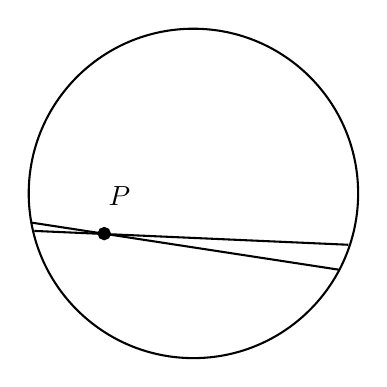
\begin{tikzpicture}[x=0.75pt,y=0.75pt,yscale=-1,xscale=1]
%uncomment if require: \path (0,238); %set diagram left start at 0, and has height of 238

%Shape: Circle [id:dp46714741031721685] 
\draw   (269,118.35) .. controls (269,74.53) and (304.53,39) .. (348.35,39) .. controls (392.18,39) and (427.71,74.53) .. (427.71,118.35) .. controls (427.71,162.18) and (392.18,197.71) .. (348.35,197.71) .. controls (304.53,197.71) and (269,162.18) .. (269,118.35) -- cycle ;
%Shape: Circle [id:dp5515785641251634] 
\draw  [fill={rgb, 255:red, 0; green, 0; blue, 0 }  ,fill opacity=1 ] (302.67,137.71) .. controls (302.67,136.22) and (303.88,135) .. (305.38,135) .. controls (306.88,135) and (308.1,136.22) .. (308.1,137.71) .. controls (308.1,139.21) and (306.88,140.43) .. (305.38,140.43) .. controls (303.88,140.43) and (302.67,139.21) .. (302.67,137.71) -- cycle ;
%Straight Lines [id:da3733346667505719] 
\draw    (271.68,136.42) -- (423.01,143.09) ;
%Straight Lines [id:da6048790919807321] 
\draw    (270.35,132.42) -- (418.35,155.09) ;

% Text Node
\draw (306,113.73) node [anchor=north west][inner sep=0.75pt]    {$P$};


\end{tikzpicture}

        \end{center}
    \end{vd}
    \begin{loigiai}
        Kí hiệu $a$ là khoảng cách từ điểm $P$ tới mảng $A$, $b$ là khoảng cách từ điểm $P$ tới mảng $B$ như trên hình vẽ. (Vì hình nón hẹp, nên có thể coi mảng $A$ và mảng $B$ có diện tích nhỏ, có thể coi khoảng cách từ $P$ tới một điểm bất kì trong mảng là khoảng cách từ $P$ tới mảng đó). Ta xét các đáy vuông góc với trục hình nón là $A'$ và $B'$ như trên hình. Tỉ lệ diện tích của $A'$ và $B'$ sẽ là $\dfrac{a^2}{b^2}$, bởi vì diện tích tỉ lệ với độ dài bình phương. Điểm mấu chốt cần nhận ra ở đây là góc giữa mặt $A$ và mặt $A'$ bằng góc giữa mặt $B$ và mặt $B'$. Điều này là đúng bởi vì $A'$ và $B'$ cùng vuông góc với trục hình nón, còn $A$ và $B$ thì tạo với trục hình nón các góc bằng nhau, do đường thẳng $AB$ là dây cung của đường tròn. Tỉ lệ diện tích của mảng $A$ so với mảng $B$ bằng với lại tỉ lệ diện tích của mảng $A'$ so với mảng $B'$ và bằng $\dfrac{a^2}{b^2}$. Mà điện tích lại tỉ lệ với diện tích nên điện tích mảng $A$ bằng $\dfrac{a^2}{b^2}$ lần điện tích của mảng $B$. 
        \begin{center}
            

\tikzset{every picture/.style={line width=0.75pt}} %set default line width to 0.75pt        

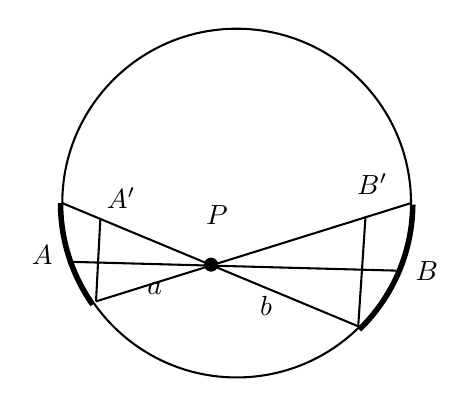
\begin{tikzpicture}[x=0.75pt,y=0.75pt,yscale=-1,xscale=1]
%uncomment if require: \path (0,238); %set diagram left start at 0, and has height of 238

%Shape: Circle [id:dp46714741031721685] 
\draw   (269.98,123.08) .. controls (269.98,76.68) and (307.59,39.07) .. (353.99,39.07) .. controls (400.39,39.07) and (438,76.68) .. (438,123.08) .. controls (438,169.48) and (400.39,207.09) .. (353.99,207.09) .. controls (307.59,207.09) and (269.98,169.48) .. (269.98,123.08) -- cycle ;
%Shape: Circle [id:dp5515785641251634] 
\draw  [fill={rgb, 255:red, 0; green, 0; blue, 0 }  ,fill opacity=1 ] (338.79,152.75) .. controls (338.79,151.16) and (340.08,149.88) .. (341.67,149.88) .. controls (343.26,149.88) and (344.54,151.16) .. (344.54,152.75) .. controls (344.54,154.34) and (343.26,155.62) .. (341.67,155.62) .. controls (340.08,155.62) and (338.79,154.34) .. (338.79,152.75) -- cycle ;
%Straight Lines [id:da3733346667505719] 
\draw    (286.23,170.44) -- (438,123.08) ;
%Straight Lines [id:da6048790919807321] 
\draw    (269.98,123.08) -- (412.56,182.44) ;
%Straight Lines [id:da32951233402203317] 
\draw    (288.34,130.21) -- (286.23,170.44) ;
%Straight Lines [id:da09769199632318037] 
\draw    (416.09,129.5) -- (412.56,182.44) ;
%Straight Lines [id:da6143629836842865] 
\draw    (430.92,155.62) -- (274.23,151.38) ;
%Shape: Arc [id:dp9065945184915425] 
\draw  [draw opacity=0][line width=1.5]  (284.35,172.17) .. controls (274.57,158.31) and (268.82,141.4) .. (268.8,123.15) -- (353.99,123.08) -- cycle ; \draw  [line width=1.5]  (284.35,172.17) .. controls (274.57,158.31) and (268.82,141.4) .. (268.8,123.15) ;
%Shape: Arc [id:dp41297456161672663] 
\draw  [draw opacity=0][line width=1.5]  (439.18,123.79) .. controls (438.98,147.52) and (429.09,168.94) .. (413.26,184.28) -- (353.99,123.08) -- cycle ; \draw  [line width=1.5]  (439.18,123.79) .. controls (438.98,147.52) and (429.09,168.94) .. (413.26,184.28) ;

% Text Node
\draw (337.74,122.87) node [anchor=north west][inner sep=0.75pt]    {$P$};
% Text Node
\draw (253.81,142.28) node [anchor=north west][inner sep=0.75pt]    {$A$};
% Text Node
\draw (438.67,149.69) node [anchor=north west][inner sep=0.75pt]    {$B$};
% Text Node
\draw (289.95,114.4) node [anchor=north west][inner sep=0.75pt]    {$A'$};
% Text Node
\draw (410.56,107.34) node [anchor=north west][inner sep=0.75pt]    {$B'$};
% Text Node
\draw (309.51,159.92) node [anchor=north west][inner sep=0.75pt]    {$a$};
% Text Node
\draw (363.86,166.27) node [anchor=north west][inner sep=0.75pt]    {$b$};


\end{tikzpicture}

        \end{center}
        Điện trường do từng mảng gây ra tại $P$ tuân theo biểu thức $E=\dfrac{q}{4\pi\varepsilon_0 r^2}$. Do đó mặc dù điện tích của $A$ bằng $\dfrac{a^2}{b^2}$ lần điện tích của $B$, nhưng giá trị $r^2$ cho mảng $A$ lại cũng bằng $\dfrac{a^2}{b^2}$ giá trị $r^2$ của mảng $B$ nên kết quả là cường độ điện trường do mảng $A$ gây ra có độ lớn bằng với cường độ điện trường do mảng $B$ gây ra ở $P$. Điện trường do hai mảng gây ra có hướng ngược chiều nhau nên chúng triệt tiêu lẫn nhau. Một quả cầu có thể chia ra làm nhiều mảng bị giới hạn bởi các mặt nón như vậy, và điện trường do các mặt nón đó từng đôi một triệt tiêu lẫn nhau. Do đó, điện trường tổng hợp tại điểm $P$ bằng không. Điều này là đúng cho một điểm $P$ bất kì bên trong quả cầu.
    \end{loigiai}
    
    
    \begin{vd}[Phân bố điện tích trên một đĩa tròn]
        Có một cách khá ``mẹo'' để tìm được phân bố điện tích trên một chiếc đĩa tròn phẳng dẫn điện với bán kính $R$ và tổng điện tích $Q$. Mục tiêu của chúng ta là tìm ra một phân bố điện tích sao cho điện trường tại một điểm trên bề mặt chiếc đĩa vuông góc với bề mặt chiếc đĩa (thành phần điện trường song song với bề mặt chiếc đĩa bằng không). Như đã chứng minh trong bài \ref{cb8}, điện trường tại một điểm $P$ bất kì bên trong một vỏ cầu tích điện đều trên bề mặt thì bằng không. Xét một phân bố điện tích khác bằng cách chiếu các điện tích trên bề mặt vỏ cầu xuống mặt phẳng đi qua $P$ và tâm vỏ cầu. Chứng minh rằng phân bố điện tích này có những tính chất của phân bố mà chúng ta đang tìm, từ đó suy ra phân bố điện tích trên một chiếc đĩa tròn dẫn điện. 
    \end{vd}
    \begin{loigiai}
    \hfill\\
    \begin{center}
        

\tikzset{every picture/.style={line width=0.75pt}} %set default line width to 0.75pt        

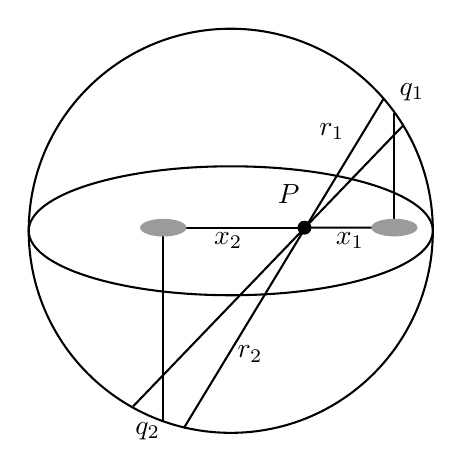
\begin{tikzpicture}[x=0.75pt,y=0.75pt,yscale=-1,xscale=1]
%uncomment if require: \path (0,238); %set diagram left start at 0, and has height of 238

%Shape: Circle [id:dp6718340227215969] 
\draw   (258,111.35) .. controls (258,57.59) and (301.59,14) .. (355.35,14) .. controls (409.12,14) and (452.71,57.59) .. (452.71,111.35) .. controls (452.71,165.12) and (409.12,208.71) .. (355.35,208.71) .. controls (301.59,208.71) and (258,165.12) .. (258,111.35) -- cycle ;
%Shape: Ellipse [id:dp03679207536578666] 
\draw   (258,111.35) .. controls (258,94.2) and (301.59,80.29) .. (355.35,80.29) .. controls (409.12,80.29) and (452.71,94.2) .. (452.71,111.35) .. controls (452.71,128.51) and (409.12,142.41) .. (355.35,142.41) .. controls (301.59,142.41) and (258,128.51) .. (258,111.35) -- cycle ;
%Shape: Circle [id:dp6201165347005493] 
\draw  [fill={rgb, 255:red, 0; green, 0; blue, 0 }  ,fill opacity=1 ] (388,109.85) .. controls (388,108.28) and (389.28,107) .. (390.85,107) .. controls (392.43,107) and (393.71,108.28) .. (393.71,109.85) .. controls (393.71,111.43) and (392.43,112.71) .. (390.85,112.71) .. controls (389.28,112.71) and (388,111.43) .. (388,109.85) -- cycle ;
%Straight Lines [id:da118178901959902] 
\draw    (429.06,47.59) -- (332.71,206.48) ;
%Straight Lines [id:da07650261292657179] 
\draw    (308.26,195.99) -- (438.26,60.79) ;
%Straight Lines [id:da1616088174307333] 
\draw    (434.18,54.47) -- (434.18,109.8) ;
%Straight Lines [id:da46335539841964213] 
\draw    (390.85,109.85) -- (434.18,109.8) ;
%Straight Lines [id:da3543480330279791] 
\draw    (322.85,109.85) -- (390.85,109.85) ;
%Straight Lines [id:da9787802557447067] 
\draw    (322.85,109.85) -- (322.85,203.14) ;
%Shape: Ellipse [id:dp7676571893601905] 
\draw  [draw opacity=0][fill={rgb, 255:red, 155; green, 155; blue, 155 }  ,fill opacity=1 ] (311.68,109.85) .. controls (311.68,107.51) and (316.68,105.61) .. (322.85,105.61) .. controls (329.02,105.61) and (334.02,107.51) .. (334.02,109.85) .. controls (334.02,112.2) and (329.02,114.1) .. (322.85,114.1) .. controls (316.68,114.1) and (311.68,112.2) .. (311.68,109.85) -- cycle ;
%Shape: Ellipse [id:dp6842573741204465] 
\draw  [draw opacity=0][fill={rgb, 255:red, 155; green, 155; blue, 155 }  ,fill opacity=1 ] (423.01,109.8) .. controls (423.01,107.46) and (428.01,105.56) .. (434.18,105.56) .. controls (440.35,105.56) and (445.35,107.46) .. (445.35,109.8) .. controls (445.35,112.15) and (440.35,114.05) .. (434.18,114.05) .. controls (428.01,114.05) and (423.01,112.15) .. (423.01,109.8) -- cycle ;

% Text Node
\draw (376.51,87.71) node [anchor=north west][inner sep=0.75pt]    {$P$};
% Text Node
\draw (396.51,58.05) node [anchor=north west][inner sep=0.75pt]    {$r_{1}$};
% Text Node
\draw (357.17,165.38) node [anchor=north west][inner sep=0.75pt]    {$r_{2}$};
% Text Node
\draw (404.51,110.71) node [anchor=north west][inner sep=0.75pt]    {$x_{1}$};
% Text Node
\draw (345.84,110.71) node [anchor=north west][inner sep=0.75pt]    {$x_{2}$};
% Text Node
\draw (435.17,38.71) node [anchor=north west][inner sep=0.75pt]    {$q_{1}$};
% Text Node
\draw (307.84,202.05) node [anchor=north west][inner sep=0.75pt]    {$q_{2}$};


\end{tikzpicture}

    \end{center}
        Nhớ lại lời giải cho bài toán \ref{cb8}, chúng ta đã chứng minh vì sao điện trường bên trong vỏ cầu lại bằng không. Trên hình vẽ, ta thấy hai hình nón bao quanh hai mảng $q_1$ và $q_2$ là đồng dạng, cho nên diện tích hai mảng (cũng như là điện tích) tỉ lệ với $\dfrac{{r_1}^2}{{r_2}^2}$. Do điện trường do từng mảng gây ra tại $P$ lại tỉ lệ nghịch với khoảng cách của từng mảng tới $P$ theo định luật Coulomb, kết quả là điện trường do hai mảng gây ra có độ lớn bằng nhau và ngược chiều nhau, nên điện trường tổng hợp tại $P$ bằng không. Ta có thể chia vỏ cầu thành từng cặp các mảng đối xứng nhau như $q_1$ và $q_2$, và điện trường của từng cặp sẽ triệt tiêu lẫn nhau, vậy nên điện trường tổng hợp do cả vỏ cầu gây ra tại $P$ bằng không.\\
        Bây giờ chúng ta sẽ chiếu các điện tích của các mạng $q_1$ và $q_2$ lên mặt phẳng đi qua $P$ và tâm vỏ cầu.\\
        Các điện tích $q_1$ và $q_2$ sẽ được chiếu lên các vị trí như trên hình. Điện trường theo phương nằm ngang do các điện tích được chiếu lên gây ra tại điểm $P$ sẽ có độ lớn lần lượt là $\dfrac{q_1}{4\pi\varepsilon_0 {x_1}^2}$ và $\dfrac{q_2}{4\pi\varepsilon_0 {x_2}^2}$. Từ các tam giác đồng dạng trong hình, ta thấy được $\dfrac{x_1}{x_2}=\dfrac{r_1}{r_2}$. Vậy nên điện trường do điện tích gây ra tại $P$ lại triệt tiêu lẫn nhau, điện trường theo phương nằm ngang tại điểm $P$ bằng không. Đây chính là tính chất cần có của phân bố điện tích chúng ta đang cần tìm.
        \begin{center}
            

\tikzset{every picture/.style={line width=0.75pt}} %set default line width to 0.75pt        

\begin{tikzpicture}[x=0.75pt,y=0.75pt,yscale=-1,xscale=1]
%uncomment if require: \path (0,238); %set diagram left start at 0, and has height of 238

%Shape: Circle [id:dp6477351268867286] 
\draw   (250.67,116.86) .. controls (250.67,60.6) and (296.27,14.99) .. (352.53,14.99) .. controls (408.79,14.99) and (454.4,60.6) .. (454.4,116.86) .. controls (454.4,173.12) and (408.79,218.73) .. (352.53,218.73) .. controls (296.27,218.73) and (250.67,173.12) .. (250.67,116.86) -- cycle ;
%Straight Lines [id:da9947060585834728] 
\draw    (250.67,116.86) -- (454.4,116.86) ;
%Straight Lines [id:da6474936030533343] 
\draw    (352.53,14.99) -- (352.53,116.86) ;
%Straight Lines [id:da849787006711521] 
\draw    (352.53,116.86) -- (426.7,48.29) ;
%Straight Lines [id:da02616449568002066] 
\draw [line width=2.25]    (418.7,39.62) -- (435.37,57.62) ;
%Straight Lines [id:da4863337237680685] 
\draw    (426.7,48.29) -- (426.7,116.29) ;
%Straight Lines [id:da79610995061943] 
\draw [line width=2.25]    (418.04,116.96) -- (434.7,116.96) ;
%Shape: Arc [id:dp2516106990306459] 
\draw  [draw opacity=0] (352.24,98.36) .. controls (352.34,98.36) and (352.44,98.36) .. (352.53,98.36) .. controls (357.72,98.36) and (362.4,100.49) .. (365.76,103.92) -- (352.53,116.86) -- cycle ; \draw   (352.24,98.36) .. controls (352.34,98.36) and (352.44,98.36) .. (352.53,98.36) .. controls (357.72,98.36) and (362.4,100.49) .. (365.76,103.92) ;

% Text Node
\draw (430.36,31.07) node [anchor=north west][inner sep=0.75pt]    {$\mathrm{d} A$};
% Text Node
\draw (387.03,123.4) node [anchor=north west][inner sep=0.75pt]    {$\mathrm{d} A\cos \theta $};
% Text Node
\draw (389.69,100.07) node [anchor=north west][inner sep=0.75pt]    {$r$};
% Text Node
\draw (335.69,50.07) node [anchor=north west][inner sep=0.75pt]    {$R$};
% Text Node
\draw (359.69,82.73) node [anchor=north west][inner sep=0.75pt]    {$\theta $};
% Text Node
\draw (263.03,119.67) node [anchor=north west][inner sep=0.75pt]   [align=left] {Đĩa};


\end{tikzpicture}

        \end{center}
        Ta có thể biểu diễn phân bố này như là một hàm theo $r$ như trên hình vẽ. Xét một đơn vị diện tích $\dd A$ trên vỏ cầu. Phần diện tích của hình chiếu của $\dd A$ trên mặt phẳng sẽ là $\dd A'=\dd A\cos\theta$. Mật độ điện tích của vỏ cầu là $\sigma$. Điện tích của phần diện tích $\dd A$ là 
        \begin{equation}
            \dd q=\sigma\dd A.
        \end{equation}
        Mật độ điện tích tại $\dd A'$ là
        \begin{equation}
        \begin{aligned}
            \sigma'(r)&=\dfrac{\dd q}{\dd A'}\\
            &=\dfrac{\sigma}{\cos\theta}\\
            &=\dfrac{\sigma R}{\sqrt{R^2-r^2}}.
        \end{aligned}
        \end{equation}
        Tổng điện tích của đĩa là $Q$ nên ta có
        \begin{equation}
            \begin{aligned}
               Q&=\int_0^R\sigma'(r)2\pi r\dd r\\
               &=\int_0^R\dfrac{\sigma R}{\sqrt{R^2-r^2}}2\pi r\dd r\\
               &=\left. -2\pi \sigma R\sqrt{R^2-r^2}\right|_0^R=2\pi\sigma R^2.
            \end{aligned}
        \end{equation}
        Từ đó suy ra $\sigma=\dfrac{Q}{2\pi R^2}$, phân bố điện tích của đĩa tròn sẽ là 
        \begin{equation}
            \sigma_d(r)=\dfrac{Q}{2\pi R\sqrt{R^2-r^2}}.
        \end{equation}
        Chúng ta có thể tìm ra được mối quan hệ giữa $\sigma$ và $Q$ bằng một cách khác không sử dụng tích phân. Hãy để ý rằng khi ta chiếu điện tích của vỏ cầu xuống mặt phẳng, tổng điện tích không đổi. Vậy nên $Q=\sigma 2\pi R^2$, suy ra $\sigma=\dfrac{Q}{2\pi R^2}$  (ở đây ta chỉ xét một nửa của vỏ cầu phía trên, do tính đối xứng nên việc bỏ qua nửa vỏ cầu bên dưới không ảnh hưởng đến kết quả cuối cùng).\\
        Mật độ điện tích tại phần rìa của chiếc đĩa tiến tới vô cùng, tuy nhiên tổng điện tích của đĩa thì lại là một giá trị hữu hạn. Mật độ điện tích tăng khi $r$ tăng, điều này là dễ hiểu vì các điện tích đẩy nhau nên tại phần rìa của đĩa các điện tích sẽ tập trung hơn. 
    \end{loigiai}
    
    
    \begin{vd}[Điện thế của quả cầu]
    Có một quả cầu kim loại lớn có bán kính $10\dv{m}$ và ban đầu có điện thế bằng không và rất nhiều những quả cầu nhỏ hơn bán kính $1\dv{m}$ ban đầu được tích điện đến điện thế $10\dv{V}$. Quả cầu lớn lần lượt được nối với các quả cầu nhỏ qua một dây dẫn mảnh dài. Trong quá trình đó các quả cầu được đặt cách xa nhau sao cho điện tích vẫn phân bố đều trên mỗi quả cầu sau mỗi lần như vậy. Hỏi quả cầu lớn phải nối với bao nhiêu quả cầu nhỏ để có thể đạt đến điện thế $9\dv{V}$?
    \end{vd}
    \begin{loigiai}
    Điện tích của mỗi quả cầu nhỏ là $q$, điện tích quả cầu lớn là $Q$. Mỗi lần quả cầu lớn nối với quả cầu nhỏ thì hai quả cầu trao đổi điện tích đến khi điện thế hai quả cầu bằng nhau. Điện thế của các quả cầu tỉ lệ với $\dfrac{q}{r}$.
    Ta có:
    \begin{equation*}
    \begin{aligned}
        &\frac{Q_{n+1}}{R}=\dfrac{Q_n+q-Q_{n+1}}{r}\\
        \Leftrightarrow \ & Q_{n+1}=\tron{Q_{n}+q}\dfrac{R}{R+r},
    \end{aligned}
    \end{equation*}
    với $Q_0=0$. \\
    Đặt $\dfrac{R}{R+r}=k$, ta có:
    \begin{equation*}
    \begin{aligned}
          Q_{n+1}&=q\tron{k^n+...+k}\\
          &=q\tron{k\dfrac{k^n-1}{k-1}}.
    \end{aligned}
    \end{equation*}
    Để điện thế quả cầu đạt tới $9\dv{V}$:
    \begin{equation*}
        \begin{aligned}
            \frac{Q_n}{R}=\frac{9}{10}\frac{q}{r}
            \Leftrightarrow q&\tron{k\dfrac{k^n-1}{k-1}}=9q\\
            \Leftrightarrow n&=\log_k\tron{\frac{9(k-1)}{k}+1}\\
            &=24,16\ .
        \end{aligned}
    \end{equation*}
    Vậy quả cầu lớn cần tiếp xúc với 25 quả cầu để đạt đến hiệu điện thế $9\dv{V}$.
    \end{loigiai}
    
\begin{vd}[Tụ điện phẳng trong bồn chứa điện môi (G)]
    Một tụ điện phẳng song song với bản tụ hình vuông có cạnh là $L$ và khoảng cách giữa hai bản tụ là $d$ được tích điện tới hiệu điện thế $V$ rồi ngắt khỏi nguồn. Sau đó nó được nhúng thẳng đứng xuống một bể rất lớn chứa chất lỏng điện môi với hằng số điện môi $\varepsilon$ và khối lượng riêng $\rho$ cho đến khi chất lỏng chiếm một nửa thể tích tụ như hình vẽ.
    \begin{center}


\tikzset{every picture/.style={line width=0.75pt}} %set default line width to 0.75pt        

\begin{tikzpicture}[x=0.75pt,y=0.75pt,yscale=-1,xscale=1]
%uncomment if require: \path (0,422); %set diagram left start at 0, and has height of 422

%Shape: Polygon [id:ds7588791827739569] 
\draw  [draw opacity=0][fill={rgb, 255:red, 155; green, 155; blue, 155 }  ,fill opacity=0.5 ] (299.8,150.4) -- (329.8,150.4) -- (329.6,210) -- (409.8,210.2) -- (409.6,291.2) -- (219.8,291.2) -- (219.6,210.2) -- (299.6,210) -- cycle ;
%Straight Lines [id:da7517226553205549] 
\draw    (220,137.56) -- (220,291.2) ;
%Straight Lines [id:da608794999274314] 
\draw    (409.8,291.2) -- (220,291.2) ;
%Straight Lines [id:da8033275110936606] 
\draw    (409.8,137.56) -- (409.8,291.2) ;
%Straight Lines [id:da28879179040321756] 
\draw    (300,70.4) -- (300,230.2) ;
%Straight Lines [id:da3709449594587153] 
\draw    (330,70.4) -- (330,230.2) ;
%Straight Lines [id:da006711851193644369] 
\draw    (329.8,150.4) -- (353.8,150.4) ;
%Straight Lines [id:da885352342345394] 
\draw    (330,230.2) -- (354,230.2) ;
%Straight Lines [id:da7609671512025402] 
\draw    (353.8,153.4) -- (353.8,227.2) ;
\draw [shift={(353.8,230.2)}, rotate = 270] [fill={rgb, 255:red, 0; green, 0; blue, 0 }  ][line width=0.08]  [draw opacity=0] (10.72,-5.15) -- (0,0) -- (10.72,5.15) -- (7.12,0) -- cycle    ;
\draw [shift={(353.8,150.4)}, rotate = 90] [fill={rgb, 255:red, 0; green, 0; blue, 0 }  ][line width=0.08]  [draw opacity=0] (10.72,-5.15) -- (0,0) -- (10.72,5.15) -- (7.12,0) -- cycle    ;
%Straight Lines [id:da23662723460306978] 
\draw    (327,65.4) -- (303,65.4) ;
\draw [shift={(300,65.4)}, rotate = 360] [fill={rgb, 255:red, 0; green, 0; blue, 0 }  ][line width=0.08]  [draw opacity=0] (7.14,-3.43) -- (0,0) -- (7.14,3.43) -- (4.74,0) -- cycle    ;
\draw [shift={(330,65.4)}, rotate = 180] [fill={rgb, 255:red, 0; green, 0; blue, 0 }  ][line width=0.08]  [draw opacity=0] (7.14,-3.43) -- (0,0) -- (7.14,3.43) -- (4.74,0) -- cycle    ;


% Text Node
\draw (357,168.4) node [anchor=north west][inner sep=0.75pt]    {$\dfrac{L}{2}$};
% Text Node
\draw (309,45.4) node [anchor=north west][inner sep=0.75pt]    {$d$};


\end{tikzpicture}

    \end{center}
    \begin{enumerate}[1)]
        \item Tính điện dung của tụ điện.
        \item Tính độ lớn của điện trường giữa hai bản tụ.
        \item Tìm sự phân bố điện tích trên hai bản tụ.
        \item Tìm độ cao dâng lên của chất lỏng trong tụ so với chất lỏng trong bình chứa.
    \end{enumerate}
\end{vd}
\begin{loigiai}
\begin{enumerate}[1)]
   \item Điện dung của hệ tụ điện song song và bình chứa điện môi chỉ đơn giản là tổng điện dung của hai tụ mắc song song:
        $$C = \dfrac{L(L/2)}{4\pi d} + \dfrac{\varepsilon L(L/2)}{4\pi d} = \dfrac{L^2}{8\pi d} (1+\varepsilon) \equiv C_0\dfrac{1+\varepsilon}{2}.$$
    \item  Điện tích trên tụ không bị thay đổi khi nhúng tụ vào bể chứa nhưng thế năng tích trữ giữa hai bản tụ thì có. Sau khi được nạp bởi nguồn, $Q=C_0 V$ Nhúng một nửa chiều cao của tụ $L/2$ vào bồn chứa, điện dung của tụ thay đổi từ $C_0$ đến $C_0(1+\varepsilon)/2$. Hiệu điện thế giữa chúng lúc sau $V’$ là:
           $$C_0V = C_0\dfrac{1+\varepsilon}{2}V’.$$
           Do đó:
           $$V’ = \dfrac{2}{1+\varepsilon}V,$$
           và do $|V| = |E|d$ nên
            $$E = \dfrac{2}{1+\varepsilon} \dfrac{V}{d}.$$
    \item Từ phương trình Maxwell $\nabla\cdot D = 4\pi\rho$, chúng ta tìm ra $D = 4\pi\sigma$ nhưng $D = \varepsilon E$ nên
    $$E = \dfrac{4\pi\sigma}{\varepsilon}.$$
    Từ phần $(2)$ ta đã tìm được: 
    $$\sigma = \dfrac{2\varepsilon}{4\pi(1+\varepsilon)} \dfrac{V}{d}$$
khi chất lỏng ngập đến giữa tụ.\\ Mật độ điện mặt tại nơi không có chất lỏng là:
    $$\sigma = \dfrac{2}{4\pi(1+\varepsilon)} \dfrac{V}{d}.$$
    \item Để tìm ra chênh lệch độ cao mực chất lỏng trong tụ và trong bể chứa bên ngoài, chúng ta tính tổng thế năng trọng trường của chất lỏng và năng lượng điện trường tích trên tụ. Gọi độ chênh lệch chiều cao là $h$ và một độ thay đổi độ cao nhỏ $\zeta$ như hình vẽ. Thế năng trọng trường của chất lỏng được tính bằng tích phân 
      $$\int_{0}^{h+\zeta}\rho gL d\,x\,\dd x = \rho g \dfrac{(h+\zeta)^2Ld}{2}.$$
       \begin{center}
            

\tikzset{every picture/.style={line width=0.75pt}} %set default line width to 0.75pt        

\begin{tikzpicture}[x=0.75pt,y=0.75pt,yscale=-1,xscale=1]
%uncomment if require: \path (0,422); %set diagram left start at 0, and has height of 422

%Shape: Polygon [id:ds7602987343581558] 
\draw  [draw opacity=0][fill={rgb, 255:red, 155; green, 155; blue, 155 }  ,fill opacity=0.5 ] (299.8,150.4) -- (329.8,150.4) -- (329.6,210) -- (409.8,210.2) -- (409.6,291.2) -- (219.8,291.2) -- (219.6,210.2) -- (299.6,210) -- cycle ;
%Shape: Sine Wave Form [id:dp9265135175779409] 
\draw   (301.82,148.06) .. controls (303.67,145.42) and (304.53,145.41) .. (306.29,148.08) .. controls (308.05,150.75) and (308.9,150.77) .. (310.77,148.1) ;
%Shape: Sine Wave Form [id:dp3721424152245498] 
\draw   (310.82,148.06) .. controls (312.67,145.42) and (313.53,145.41) .. (315.29,148.08) .. controls (317.05,150.75) and (317.9,150.77) .. (319.77,148.1) ;
%Shape: Sine Wave Form [id:dp5210302132347915] 
\draw   (319.82,148.06) .. controls (321.67,145.42) and (322.53,145.41) .. (324.29,148.08) .. controls (326.05,150.75) and (326.9,150.77) .. (328.77,148.1) ;

%Straight Lines [id:da6556588775482208] 
\draw    (220,137.56) -- (220,291.2) ;
%Straight Lines [id:da2507747172556749] 
\draw    (409.8,291.2) -- (220,291.2) ;
%Straight Lines [id:da3622638859499685] 
\draw    (409.8,137.56) -- (409.8,291.2) ;
%Straight Lines [id:da7573141890185227] 
\draw    (300,70.4) -- (300,230.2) ;
%Straight Lines [id:da13394710382284236] 
\draw    (330,70.4) -- (330,230.2) ;
%Straight Lines [id:da09363042769351826] 
\draw    (329.8,150.4) -- (353.8,150.4) ;
%Straight Lines [id:da15844310691649666] 
\draw    (330,230.2) -- (354,230.2) ;
%Straight Lines [id:da5428183923971306] 
\draw    (353.8,153.4) -- (353.8,227.2) ;
\draw [shift={(353.8,230.2)}, rotate = 270] [fill={rgb, 255:red, 0; green, 0; blue, 0 }  ][line width=0.08]  [draw opacity=0] (10.72,-5.15) -- (0,0) -- (10.72,5.15) -- (7.12,0) -- cycle    ;
\draw [shift={(353.8,150.4)}, rotate = 90] [fill={rgb, 255:red, 0; green, 0; blue, 0 }  ][line width=0.08]  [draw opacity=0] (10.72,-5.15) -- (0,0) -- (10.72,5.15) -- (7.12,0) -- cycle    ;
%Shape: Sine Wave Form [id:dp2066796886763671] 
\draw   (300.82,144.26) .. controls (302.81,141.42) and (303.74,141.41) .. (305.63,144.28) .. controls (307.52,147.15) and (308.42,147.17) .. (310.43,144.3) ;
%Shape: Sine Wave Form [id:dp3009934611124063] 
\draw   (310.49,144.26) .. controls (312.48,141.42) and (313.4,141.41) .. (315.29,144.28) .. controls (317.19,147.15) and (318.09,147.17) .. (320.1,144.3) ;
%Shape: Sine Wave Form [id:dp4212523783536659] 
\draw   (320.16,144.26) .. controls (322.15,141.42) and (323.07,141.41) .. (324.96,144.28) .. controls (326.85,147.15) and (327.75,147.17) .. (329.76,144.3) ;

%Shape: Sine Wave Form [id:dp008294576835681466] 
\draw   (302.82,140.06) .. controls (304.67,137.42) and (305.53,137.41) .. (307.29,140.08) .. controls (309.05,142.75) and (309.9,142.77) .. (311.77,140.1) ;
%Shape: Sine Wave Form [id:dp16870384965352647] 
\draw   (311.82,140.06) .. controls (313.67,137.42) and (314.53,137.41) .. (316.29,140.08) .. controls (318.05,142.75) and (318.9,142.77) .. (320.77,140.1) ;
%Shape: Sine Wave Form [id:dp019431373960939524] 
\draw   (320.82,140.06) .. controls (322.67,137.42) and (323.53,137.41) .. (325.29,140.08) .. controls (327.05,142.75) and (327.9,142.77) .. (329.77,140.1) ;

%Straight Lines [id:da11546994351349116] 
\draw    (327,65.4) -- (303,65.4) ;
\draw [shift={(300,65.4)}, rotate = 360] [fill={rgb, 255:red, 0; green, 0; blue, 0 }  ][line width=0.08]  [draw opacity=0] (7.14,-3.43) -- (0,0) -- (7.14,3.43) -- (4.74,0) -- cycle    ;
\draw [shift={(330,65.4)}, rotate = 180] [fill={rgb, 255:red, 0; green, 0; blue, 0 }  ][line width=0.08]  [draw opacity=0] (7.14,-3.43) -- (0,0) -- (7.14,3.43) -- (4.74,0) -- cycle    ;


% Text Node
\draw (357,168.4) node [anchor=north west][inner sep=0.75pt]    {$\dfrac{L}{2}$};
% Text Node
\draw (279,135.4) node [anchor=north west][inner sep=0.75pt]    {$\zeta $};
% Text Node
\draw (297.23,142) node    {$\{$};
% Text Node
\draw (309,45.4) node [anchor=north west][inner sep=0.75pt]    {$d$};


\end{tikzpicture}

        \end{center}
      Do đó tổng năng lượng là:
      $$U = \dfrac{1}{2} \dfrac{Q^2}{C} + \dfrac{\rho g (h+\zeta)^2 Ld}{2}.$$
    Ở đây chúng ta phải viết lại năng lượng điện trường theo $Q$ vì năng lượng này sẽ thay đổi theo độ cao mực nước. Thế thành phần $C$ theo các tham số khác, ta có:
    $$U = \dfrac{1}{2} \dfrac{8\pi Q^2d}{L^2(1+\varepsilon) + 2L(\varepsilon-1)\zeta} + \dfrac{\rho g (h+\zeta)^2Ld}{2}.$$
    Ở vị trí cân bằng, tổng lực tác dụng lên chất lỏng bằng không nên đạo hàm của năng lượng ta tính ở trên bằng không:
    $$-\dfrac{\partial U}{\partial\zeta} = \dfrac{1}{2} \dfrac{16\pi Q^2Ld(\varepsilon-1)}{[L^2(\varepsilon+1) + 2L(\varepsilon-1)\zeta]^2} - \rho g(h+\zeta)Ld = 0.$$

    Ở vị trí cân bằng, $\zeta = 0$:
        $$\dfrac{8\pi Q^2Ld(\varepsilon-1)}{L^4(\varepsilon+1)^2} = \rho gL\,\dd h$$
    $$h = \dfrac{8\pi Q^2(\varepsilon-1)}{L^4\rho g(\varepsilon+1)^2}.$$
Viết lại phương trình trên theo $V$, ta thu được:
    $$h=\frac{V^2}{2\pi\rho g d^2}\frac{\varepsilon -1}{(\varepsilon+1)^2}.$$
    Theo một cách khác, ta có thể tính được lực bằng cách:
      $$F_h = \left(-\dfrac{\partial U}{\partial x}\right)_{x=L/2} = \dfrac{2\pi dQ^2}{L} \dfrac{(\varepsilon-1)}{[L+L(\varepsilon-1)/2]^2}.$$  
      Và trọng lượng của phần nước là:
        $$W = \rho ghLd.$$
         Từ đó ta tính ra:
         $$h = \dfrac{8\pi Q^2(\varepsilon-1)}{L^4\rho g(\varepsilon+1)^2}.$$
      cũng thu được kết quả tương tự như cách làm bên trên. 
\end{enumerate}
\end{loigiai}


\begin{vd}[Lực điện và sự giãn nở]
    \begin{enumerate}[1)]
        \item Nghiên cứu hai quả cầu điện môi với bán kính $a$, đặt cách nhau một khoảng $R\, (R\gg a)$. Một quả cầu được tích điện $q$, trong khi quả cầu còn lại được giữ trung hòa điện. Bây giờ chúng ta tăng kích thước dài của hệ lên gấp hai lần (bán kính quả cầu và khoảng cách giữa chúng tăng gấp hai lần). Để lực tương tác giữa hai quả cầu không đổi thì điện tích quả cầu $1$ phải tăng lên bao nhiêu?
        \begin{center}
            

\tikzset{every picture/.style={line width=0.75pt}} %set default line width to 0.75pt        

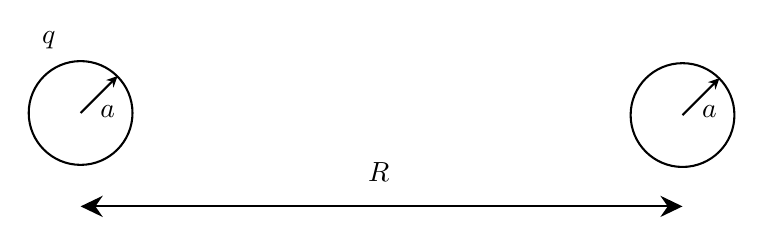
\begin{tikzpicture}[x=0.75pt,y=0.75pt,yscale=-1,xscale=1]
%uncomment if require: \path (0,465); %set diagram left start at 0, and has height of 465

%Shape: Circle [id:dp42265347563661804] 
\draw   (165,185) .. controls (165,171.19) and (176.19,160) .. (190,160) .. controls (203.81,160) and (215,171.19) .. (215,185) .. controls (215,198.81) and (203.81,210) .. (190,210) .. controls (176.19,210) and (165,198.81) .. (165,185) -- cycle ;
%Shape: Circle [id:dp49358445532785544] 
\draw   (455,186) .. controls (455,172.19) and (466.19,161) .. (480,161) .. controls (493.81,161) and (505,172.19) .. (505,186) .. controls (505,199.81) and (493.81,211) .. (480,211) .. controls (466.19,211) and (455,199.81) .. (455,186) -- cycle ;
%Straight Lines [id:da47270362610943795] 
\draw    (193,230) -- (357.6,230) -- (477,230) ;
\draw [shift={(480,230)}, rotate = 180] [fill={rgb, 255:red, 0; green, 0; blue, 0 }  ][line width=0.08]  [draw opacity=0] (10.72,-5.15) -- (0,0) -- (10.72,5.15) -- (7.12,0) -- cycle    ;
\draw [shift={(190,230)}, rotate = 0] [fill={rgb, 255:red, 0; green, 0; blue, 0 }  ][line width=0.08]  [draw opacity=0] (10.72,-5.15) -- (0,0) -- (10.72,5.15) -- (7.12,0) -- cycle    ;
%Straight Lines [id:da9999361003926563] 
\draw    (190,185) -- (205.68,169.32) ;
\draw [shift={(207.8,167.2)}, rotate = 495] [fill={rgb, 255:red, 0; green, 0; blue, 0 }  ][line width=0.08]  [draw opacity=0] (5.36,-2.57) -- (0,0) -- (5.36,2.57) -- (3.56,0) -- cycle    ;
%Straight Lines [id:da15833993928459633] 
\draw    (480,186) -- (495.68,170.32) ;
\draw [shift={(497.8,168.2)}, rotate = 495] [fill={rgb, 255:red, 0; green, 0; blue, 0 }  ][line width=0.08]  [draw opacity=0] (5.36,-2.57) -- (0,0) -- (5.36,2.57) -- (3.56,0) -- cycle    ;


% Text Node
\draw (170,144.4) node [anchor=north west][inner sep=0.75pt]    {$q$};
% Text Node
\draw (198,180) node [anchor=north west][inner sep=0.75pt]    {$a$};
% Text Node
\draw (487.9,180) node [anchor=north west][inner sep=0.75pt]    {$a$};
% Text Node
\draw (327,207.4) node [anchor=north west][inner sep=0.75pt]    {$R$};


\end{tikzpicture}
        \end{center}
        \item Bây giờ ta nghiên cứu một chiếc vòng dẫn điện làm từ dây dẫn mảnh, với $d$ là đường kính dây và $D$ là đường kính của vòng dây $(D\gg d)$. Tích điện cho vòng dây một điện tích q vừa đủ cho vòng dây đứt do lực căng tĩnh điện. Bây giờ chúng ta lại tăng kích thước dài của vòng dây lên hai lần như câu $1)$. Lúc này phải tích cho vòng dây một điện tích bằng bao nhiêu để dây đứt?
        \begin{center}
            

\tikzset{every picture/.style={line width=0.75pt}} %set default line width to 0.75pt        

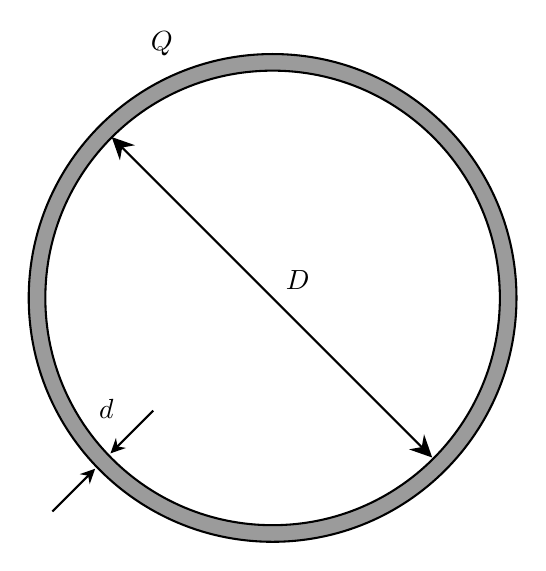
\begin{tikzpicture}[x=0.75pt,y=0.75pt,yscale=-1,xscale=1]
%uncomment if require: \path (0,575); %set diagram left start at 0, and has height of 575

%Shape: Donut [id:dp5869287598506212] 
\draw  [fill={rgb, 255:red, 155; green, 155; blue, 155 }  ,fill opacity=1 ,even odd rule] (216.6,238.1) .. controls (216.6,177.62) and (265.62,128.6) .. (326.1,128.6) .. controls (386.58,128.6) and (435.6,177.62) .. (435.6,238.1) .. controls (435.6,298.58) and (386.58,347.6) .. (326.1,347.6) .. controls (265.62,347.6) and (216.6,298.58) .. (216.6,238.1)(208.6,238.1) .. controls (208.6,173.21) and (261.21,120.6) .. (326.1,120.6) .. controls (390.99,120.6) and (443.6,173.21) .. (443.6,238.1) .. controls (443.6,302.99) and (390.99,355.6) .. (326.1,355.6) .. controls (261.21,355.6) and (208.6,302.99) .. (208.6,238.1) ;
%Straight Lines [id:da2197263355479353] 
\draw    (250.72,162.72) -- (400.88,312.88) ;
\draw [shift={(403,315)}, rotate = 225] [fill={rgb, 255:red, 0; green, 0; blue, 0 }  ][line width=0.08]  [draw opacity=0] (10.72,-5.15) -- (0,0) -- (10.72,5.15) -- (7.12,0) -- cycle    ;
\draw [shift={(248.6,160.6)}, rotate = 45] [fill={rgb, 255:red, 0; green, 0; blue, 0 }  ][line width=0.08]  [draw opacity=0] (10.72,-5.15) -- (0,0) -- (10.72,5.15) -- (7.12,0) -- cycle    ;
%Straight Lines [id:da9221036743576936] 
\draw    (250.12,310.88) -- (268.6,292.4) ;
\draw [shift={(248,313)}, rotate = 315] [fill={rgb, 255:red, 0; green, 0; blue, 0 }  ][line width=0.08]  [draw opacity=0] (7.14,-3.43) -- (0,0) -- (7.14,3.43) -- (4.74,0) -- cycle    ;
%Straight Lines [id:da15873300869830165] 
\draw    (220,341) -- (238.48,322.52) ;
\draw [shift={(240.6,320.4)}, rotate = 495] [fill={rgb, 255:red, 0; green, 0; blue, 0 }  ][line width=0.08]  [draw opacity=0] (7.14,-3.43) -- (0,0) -- (7.14,3.43) -- (4.74,0) -- cycle    ;


% Text Node
\draw (241,285.4) node [anchor=north west][inner sep=0.75pt]    {$d$};
% Text Node
\draw (331,223.4) node [anchor=north west][inner sep=0.75pt]    {$D$};
% Text Node
\draw (266,108.4) node [anchor=north west][inner sep=0.75pt]    {$Q$};


\end{tikzpicture}
        \end{center}
    \end{enumerate}

\end{vd}
\begin{loigiai}
    \begin{enumerate}[1)]
        \item Quả cầu bị tích điện sẽ hưởng ứng và làm phân cực quả cầu trung hòa do đó tạo ra một moment lưỡng cực p tỉ lệ thuận với cường độ điện trường của quả cầu tích điện:
        $$p \propto E \propto \dfrac{q}{R^2}.$$
        Lực tương tác giữa lưỡng cực điện và quả cầu tích điện bằng tích của moment lưỡng cực và gradient của cường độ điện trường tại vị trí của lưỡng cực:
       $$F \propto \dfrac{pq}{R^3} \propto \dfrac{q^2}{R^5}.$$
       Để có $F'=F$ sau khi tăng kích thước dài của hệ lên hai lần thì điện tích $q’$ phải thỏa mãn:
       $$\dfrac{q^2}{R^5} = \dfrac{q’^2}{R’^5}$$
       $$\left(\dfrac{q’}{q}\right)^2 = \left(\dfrac{R’}{R}\right)^5 = 32$$
       $$q’ = 4\sqrt{2} q.$$
       \item Điện tích $Q$ sẽ được phân bố đều dọc theo dây. Do đó lực Coulomb giữa một điểm trên vòng và phần còn lại của vòng sẽ tỉ lệ thuận với bình phương của $Q$ và tỉ lệ nghịch với bình phương đường kính vòng $D$:
       $$F_Q \propto \dfrac{Q^2}{D^2}.$$
       Khi vòng dây bị đứt, lực đàn hồi $F_e$ giới hạn dọc theo vòng sẽ là:
        $$F_e = \sigma S,$$
        trong đó $\sigma$ là sức căng cực đại, chỉ phụ thuộc vào vật liệu làm dây, và $S$ là tiết diện mặt cắt của dây. Tại thời điểm vòng dây đứt, $F_Q=F_e$, do đó cân bằng hai phương trình trên ta có:
        $$Q^2 \propto \sigma SD^2 \propto \sigma d^2D^2.$$
        Tăng kích thước dài của hệ lên hai lần cho ta:
         $$Q’ \propto d’D’ = 4dD.$$
         Do đó:
        $$Q' = 4Q.$$
    \end{enumerate}
\end{loigiai}



\begin{vd}[Hệ tụ điện không song song (G)]
\begin{enumerate}[1)]
    \item Một tụ điện được cấu tạo thành từ hai bản tụ dẫn điện hình chữ nhật với các cạnh dài lần lượt $L_1$ và $L_2$. Hai bản tụ này được đặt không song song nhau. Một cặp cạnh của tụ dài $L_1$ được đặt song song cách nhau $d_1$ và cặp cạnh $L_1$ còn lại được đặt song song và cách nhau $d_2$; trong đó $d_2>d_1$. (Xem hình vẽ)\\ %đính hình vẽ
\begin{center}


\tikzset{every picture/.style={line width=0.75pt}} %set default line width to 0.75pt        

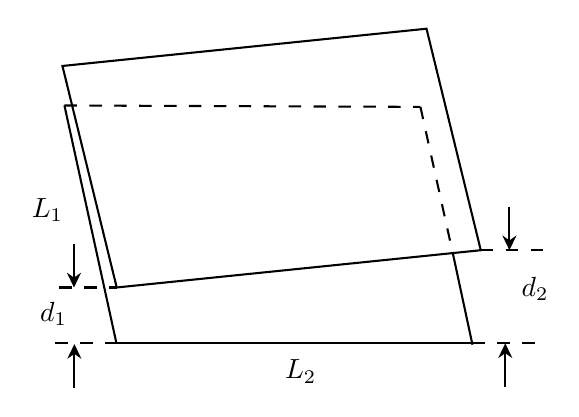
\begin{tikzpicture}[x=0.75pt,y=0.75pt,yscale=-1,xscale=1]
%uncomment if require: \path (0,490); %set diagram left start at 0, and has height of 490

%Straight Lines [id:da712602482648053] 
\draw    (159.21,151.27) -- (184.28,265.86) ;
%Straight Lines [id:da45102212002233655] 
\draw    (184.28,265.86) -- (355.8,265.86) ;
%Straight Lines [id:da19129120832648439] 
\draw    (346.8,224.6) -- (355.79,266.53) ;
%Straight Lines [id:da8526825428836884] 
\draw  [dash pattern={on 4.5pt off 4.5pt}]  (330.72,151.94) -- (346.8,224.6) ;
%Straight Lines [id:da3456668494272379] 
\draw  [dash pattern={on 4.5pt off 4.5pt}]  (159.21,151.27) -- (330.72,151.94) ;
%Shape: Parallelogram [id:dp6883692974447599] 
\draw   (333.65,114.28) -- (359.8,221) -- (184.4,238.95) -- (158.25,132.23) -- cycle ;
%Straight Lines [id:da9980615488127933] 
\draw  [dash pattern={on 4.5pt off 4.5pt}]  (156.8,238.95) -- (184.4,238.95) ;
%Straight Lines [id:da9800983319866017] 
\draw  [dash pattern={on 4.5pt off 4.5pt}]  (154.8,265.86) -- (184.28,265.86) ;
%Straight Lines [id:da513912025331484] 
\draw  [dash pattern={on 4.5pt off 4.5pt}]  (359.8,221) -- (389.8,221) ;
%Straight Lines [id:da6319286640176305] 
\draw  [dash pattern={on 4.5pt off 4.5pt}]  (355.8,265.86) -- (386.8,265.86) ;
%Straight Lines [id:da02605118085004654] 
\draw    (163.8,217.95) -- (163.8,235.95) ;
\draw [shift={(163.8,238.95)}, rotate = 270] [fill={rgb, 255:red, 0; green, 0; blue, 0 }  ][line width=0.08]  [draw opacity=0] (7.14,-3.43) -- (0,0) -- (7.14,3.43) -- (4.74,0) -- cycle    ;
%Straight Lines [id:da5604084916920165] 
\draw    (164,269.2) -- (164,287.2) ;
\draw [shift={(164,266.2)}, rotate = 90] [fill={rgb, 255:red, 0; green, 0; blue, 0 }  ][line width=0.08]  [draw opacity=0] (7.14,-3.43) -- (0,0) -- (7.14,3.43) -- (4.74,0) -- cycle    ;
%Straight Lines [id:da4315925723080418] 
\draw    (373.6,200) -- (373.6,218) ;
\draw [shift={(373.6,221)}, rotate = 270] [fill={rgb, 255:red, 0; green, 0; blue, 0 }  ][line width=0.08]  [draw opacity=0] (7.14,-3.43) -- (0,0) -- (7.14,3.43) -- (4.74,0) -- cycle    ;
%Straight Lines [id:da27425010839765407] 
\draw    (371.6,268.86) -- (371.6,286.86) ;
\draw [shift={(371.6,265.86)}, rotate = 90] [fill={rgb, 255:red, 0; green, 0; blue, 0 }  ][line width=0.08]  [draw opacity=0] (7.14,-3.43) -- (0,0) -- (7.14,3.43) -- (4.74,0) -- cycle    ;


% Text Node
\draw (146,244.4) node [anchor=north west][inner sep=0.75pt]    {$d_{1}$};
% Text Node
\draw (378,232.4) node [anchor=north west][inner sep=0.75pt]    {$d_{2}$};
% Text Node
\draw (142,194.4) node [anchor=north west][inner sep=0.75pt]    {$L_{1}$};
% Text Node
\draw (264,272.4) node [anchor=north west][inner sep=0.75pt]    {$L_{2}$};


\end{tikzpicture}
\end{center}
    Bỏ qua mọi hiệu ứng rìa, khi đặt một hiệu điện thế $V$ vào hai bản tụ, tìm điện thế ở một điểm bất kì giữa hai tụ.
    \item Tính điện dung của hệ.
\end{enumerate}
\end{vd}

\begin{loigiai}
\begin{enumerate}[1)]
\item Đặt một hệ tọa độ trụ sao cho các bản tụ nằm dọc theo phương bán kính của hệ tọa độ (xem hình vẽ). Phương trình Laplace $\nabla^2 \phi=0$ do đó:

  \begin{center}


\tikzset{every picture/.style={line width=0.75pt}} %set default line width to 0.75pt        

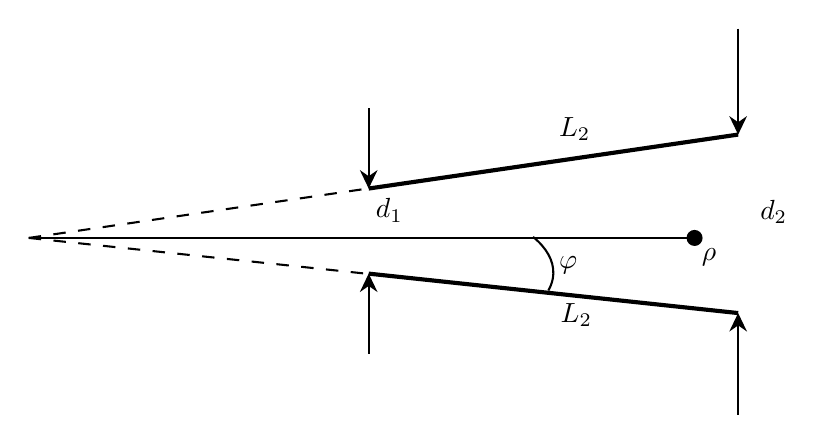
\begin{tikzpicture}[x=0.75pt,y=0.75pt,yscale=-1,xscale=1]
%uncomment if require: \path (0,463); %set diagram left start at 0, and has height of 463

%Straight Lines [id:da8888219188553073] 
\draw    (137,240) -- (457.8,240) ;
\draw [shift={(457.8,240)}, rotate = 0] [color={rgb, 255:red, 0; green, 0; blue, 0 }  ][fill={rgb, 255:red, 0; green, 0; blue, 0 }  ][line width=0.75]      (0, 0) circle [x radius= 3.35, y radius= 3.35]   ;
%Straight Lines [id:da0375644723320927] 
\draw  [dash pattern={on 4.5pt off 4.5pt}]  (137,240) -- (478.8,190.2) ;
%Straight Lines [id:da5190157214133659] 
\draw  [dash pattern={on 4.5pt off 4.5pt}]  (137,240) -- (478.8,276.2) ;
%Straight Lines [id:da37116370456208414] 
\draw [line width=1.5]    (300.8,216.2) -- (478.8,190.2) ;
%Straight Lines [id:da03708741936908044] 
\draw [line width=1.5]    (300.8,257.2) -- (478.8,276.2) ;
%Straight Lines [id:da18268352409070432] 
\draw    (300.8,177.4) -- (300.8,213.2) ;
\draw [shift={(300.8,216.2)}, rotate = 270] [fill={rgb, 255:red, 0; green, 0; blue, 0 }  ][line width=0.08]  [draw opacity=0] (8.93,-4.29) -- (0,0) -- (8.93,4.29) -- (5.93,0) -- cycle    ;
%Straight Lines [id:da7567562935874099] 
\draw    (300.8,260.2) -- (300.8,296) ;
\draw [shift={(300.8,257.2)}, rotate = 90] [fill={rgb, 255:red, 0; green, 0; blue, 0 }  ][line width=0.08]  [draw opacity=0] (8.93,-4.29) -- (0,0) -- (8.93,4.29) -- (5.93,0) -- cycle    ;
%Straight Lines [id:da7764810518012757] 
\draw    (478.8,139.2) -- (478.8,187.2) ;
\draw [shift={(478.8,190.2)}, rotate = 270] [fill={rgb, 255:red, 0; green, 0; blue, 0 }  ][line width=0.08]  [draw opacity=0] (8.93,-4.29) -- (0,0) -- (8.93,4.29) -- (5.93,0) -- cycle    ;
%Straight Lines [id:da7451709181736375] 
\draw    (478.8,279.2) -- (478.8,325.2) ;
\draw [shift={(478.8,276.2)}, rotate = 90] [fill={rgb, 255:red, 0; green, 0; blue, 0 }  ][line width=0.08]  [draw opacity=0] (8.93,-4.29) -- (0,0) -- (8.93,4.29) -- (5.93,0) -- cycle    ;
%Shape: Arc [id:dp8276494349776893] 
\draw  [draw opacity=0] (379.98,239.5) .. controls (386.38,244.69) and (390.02,250.87) .. (389.75,257.37) .. controls (389.63,260.15) and (388.81,262.81) .. (387.37,265.31) -- (333.4,255) -- cycle ; \draw   (379.98,239.5) .. controls (386.38,244.69) and (390.02,250.87) .. (389.75,257.37) .. controls (389.63,260.15) and (388.81,262.81) .. (387.37,265.31) ;


% Text Node
\draw (459.8,243.4) node [anchor=north west][inner sep=0.75pt]    {$\rho $};
% Text Node
\draw (302.8,219.6) node [anchor=north west][inner sep=0.75pt]    {$d_{1}$};
% Text Node
\draw (488,220.4) node [anchor=north west][inner sep=0.75pt]    {$d_{2}$};
% Text Node
\draw (391,180.4) node [anchor=north west][inner sep=0.75pt]    {$L_{2}$};
% Text Node
\draw (391.8,270.1) node [anchor=north west][inner sep=0.75pt]    {$L_{2}$};
% Text Node
\draw (391,247.4) node [anchor=north west][inner sep=0.75pt]    {$\varphi $};


\end{tikzpicture}
\end{center}
trở thành:
   $$\frac{1}{\rho}\frac{\partial}{\partial\rho}\left(\rho\frac{\partial\phi}{\partial\rho}\right) + \frac{1}{\rho^2}\frac{\partial^2 \phi}{\partial \varphi^2} = 0.$$
Đặt $\phi=R(\rho)\chi(\varphi)$, chúng ta có thể tách phương trình trên thành hai phương trình đạo hàm:
     $$\frac{\rho}{R} \frac{\dd}{\dd\rho}\left(\rho\frac{\dd R}{\dd\rho}\right) = n^2$$
     $$\frac{1}{\chi} \frac{\dd^2 \chi}{\dd \varphi^2} = -n^2.$$
trong đó $R$ là thành phần theo phương bán kính của điện thế, $\chi$ là thành phần theo trục đối xứng, và $n$ là một hằng số. Trong giới hạn xấp xỉ góc nhỏ (điều kiện có thể được công nhận vì chúng ta đã bỏ qua hiệu ứng rìa), chúng ta có thể công nhận $R$ không phụ thuộc vào $\rho$, do đó:
  $$\frac{\dd^2\chi}{\dd \varphi^2} =0,$$
ta có nghiệm cho phương trình này $\chi = A\varphi + B$. Từ điều kiện biên $\chi(0) = 0$, chúng ta có $B=0$, và sử dụng điều kiện biên còn lại $\chi(\varphi_0)=V$, ta tìm được:
   $$\phi = V\frac{\varphi}{\varphi_0},$$
trong đó
     $$\varphi_0 \approx \sin\varphi_0 = \frac{d_2 - d_1}{L_2},$$
\item Sử dụng kết quả của câu $1)$ và biểu thức năng lượng điện trường $U$ tích trữ trong tụ ta sẽ tính được điện dung của tụ:
    $$U= \frac{1}{2}CV^2=\frac{1}{8\pi}\int E^2 \dd^3 x.$$
Ở đây,
  $$\ot{E} = -\nabla\phi= -\frac{V}{\rho\varphi_0}\ot{e}_{\varphi}.$$
Do đó tích phân trên trở thành:
 $$\frac{1}{2} C V^{2}=\frac{1}{8 \pi} \int_{0}^{L_{1}} \int_{\rho_{1}}^{\rho_{2}} \int_{0}^{\varphi_{0}} \frac{V^{2}}{\rho^{2} \varphi_{0}^{2}} \rho \dd \varphi \dd \rho \dd z$$
 $$=\frac{1}{8 \pi} \frac{L_{1} V^{2}}{\varphi_{0}} \int_{\rho_{1}}^{\rho_{2}} \frac{\dd \rho}{\rho}=\frac{L_{1} L_{2} V^{2}}{8 \pi\left(d_{2}-d_{1}\right)} \ln \frac{d_{2} / \varphi_{0}}{d_{1} / \varphi_{0}}=\frac{L_{1} L_{2} V^{2}}{8 \pi\left(d_{2}-d_{1}\right)} \ln \frac{d_{2}}{d_{1}}.$$
Do đó điện dung tụ là:
    $$C=\frac{L_{1} L_{2}}{4 \pi\left(d_{2}-d_{1}\right)} \ln \frac{d_{2}}{d_{1}}=\frac{L_{1} L_{2}}{4 \pi\left(d_{2}-d_{1}\right)} \ln \left(1+\frac{d_{2}-d_{1}}{d_{1}}\right).$$
Trong giới hạn $d_2\rightarrow d_1=d$ (tương tự như một tụ song song), biểu thức điện dung rút gọn còn:
        $$C \approx \frac{L_1 L_2}{4\pi (d_2 -d_1)}\cdot\frac{(d_2 -d_1)}{d_1} =\frac{L_1 L_2}{4\pi d}.$$
biểu thức này tương tự như điện dung các tụ điện phẳng quen thuộc.
\end{enumerate}
\end{loigiai}


\begin{vd}[Điện tích đặt lệch]
\begin{center}
    \bf Phần I
\end{center}
Xét hai nhóm các điện tích. Nhóm $A$ gồm $N$ điện tích $q_1, q_2,\dots q_{N}$ được đặt tại các vị trí $\ot{r_1}, \ot{r_2}, \dots \ot{r_{N}}$ tương ứng. Nhóm $B$ gồm $M$ điện tích $q_1, q_2,\dots q_{M}$ được đặt tại các vị trí $\ot{r_1}, \ot{r_2}, \dots \ot{r_{M}}$ tương ứng.
\begin{enumerate}[1)]
    \item Viết biểu thức điện thế $\phi_{A}(\ot{r})$ tại vị trí $\ot{r}$ do các điện tích của nhóm $A$ gây ra.
    \item Viết biểu thức thế năng tĩnh điện $E_{B/A}$ tại nhóm $B$ do điện thế  $\phi_{A}(\ot{r})$ gây ra.
    \item Mối quan hệ giữa $E_{B/A}$ và $E_{A/B}$ là gì?
    \end{enumerate}
    \begin{center}
        \bf Phần II
    \end{center}
\begin{enumerate}[1)]
\setcounter{enumi}{3}
    \item Xét hai tấm phẳng dẫn điện như hình $(a)$. Tấm trên mang điện tích đều với mật độ điện mặt $\sigma'$ và tấm dưới được nối đất. Tìm mật độ điện tích mặt của tấm dưới và điện thế $\phi'(z)$, với $z$ là độ cao của tùy ý tính từ tấm dưới.
    \begin{center}
% Gradient Info
\tikzset {_hohk0nkfl/.code = {\pgfsetadditionalshadetransform{ \pgftransformshift{\pgfpoint{-198 bp } { 158.4 bp }  }  \pgftransformscale{1.32 }  }}}
\pgfdeclareradialshading{_892sj7syc}{\pgfpoint{160bp}{-128bp}}{rgb(0bp)=(1,1,1);
rgb(0bp)=(1,1,1);
rgb(25bp)=(0,0,0);
rgb(400bp)=(0,0,0)}
\tikzset{every picture/.style={line width=0.75pt}} %set default line width to 0.75pt        

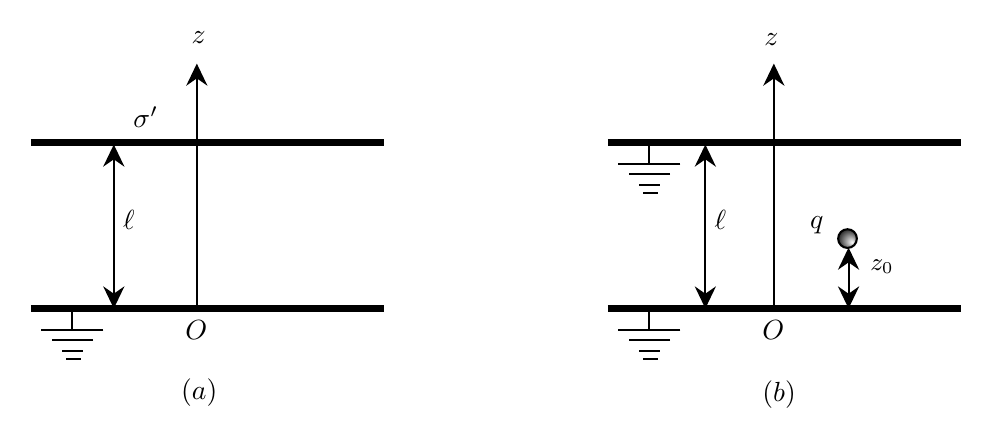
\begin{tikzpicture}[x=0.75pt,y=0.75pt,yscale=-1,xscale=1]
%uncomment if require: \path (0,300); %set diagram left start at 0, and has height of 300

%Straight Lines [id:da5744112006701443] 
\draw [line width=2.25]    (50.02,230.2) -- (220.02,230.2) ;
%Straight Lines [id:da8690459165768833] 
\draw [line width=2.25]    (50.02,150.2) -- (220.02,150.2) ;
%Straight Lines [id:da07085530429119968] 
\draw    (90.02,227.2) -- (90.02,154.2) ;
\draw [shift={(90.02,151.2)}, rotate = 450] [fill={rgb, 255:red, 0; green, 0; blue, 0 }  ][line width=0.08]  [draw opacity=0] (10.72,-5.15) -- (0,0) -- (10.72,5.15) -- (7.12,0) -- cycle    ;
\draw [shift={(90.02,230.2)}, rotate = 270] [fill={rgb, 255:red, 0; green, 0; blue, 0 }  ][line width=0.08]  [draw opacity=0] (10.72,-5.15) -- (0,0) -- (10.72,5.15) -- (7.12,0) -- cycle    ;
%Straight Lines [id:da7730834529264963] 
\draw    (130.02,231.2) -- (130.02,115.2) ;
\draw [shift={(130.02,112.2)}, rotate = 450] [fill={rgb, 255:red, 0; green, 0; blue, 0 }  ][line width=0.08]  [draw opacity=0] (10.72,-5.15) -- (0,0) -- (10.72,5.15) -- (7.12,0) -- cycle    ;
%Straight Lines [id:da6884176023142436] 
\draw    (70.02,230.53) -- (70.02,240.53) ;
%Straight Lines [id:da09371869366650887] 
\draw    (85.02,240.53) -- (55.02,240.53) ;
%Straight Lines [id:da09628245206196029] 
\draw    (80.02,245.53) -- (60.02,245.53) ;
%Straight Lines [id:da25702921235035014] 
\draw    (75.02,250.53) -- (65.02,250.53) ;
%Straight Lines [id:da720705614384034] 
\draw    (74.02,254.53) -- (67.02,254.53) ;
%Straight Lines [id:da27732417557497313] 
\draw [line width=2.25]    (328.02,230.2) -- (498.02,230.2) ;
%Straight Lines [id:da7178949508514356] 
\draw [line width=2.25]    (328.02,150.2) -- (498.02,150.2) ;
%Straight Lines [id:da0010266236395068962] 
\draw    (375.02,227.2) -- (375.02,154.2) ;
\draw [shift={(375.02,151.2)}, rotate = 450] [fill={rgb, 255:red, 0; green, 0; blue, 0 }  ][line width=0.08]  [draw opacity=0] (10.72,-5.15) -- (0,0) -- (10.72,5.15) -- (7.12,0) -- cycle    ;
\draw [shift={(375.02,230.2)}, rotate = 270] [fill={rgb, 255:red, 0; green, 0; blue, 0 }  ][line width=0.08]  [draw opacity=0] (10.72,-5.15) -- (0,0) -- (10.72,5.15) -- (7.12,0) -- cycle    ;
%Straight Lines [id:da05406519506480789] 
\draw    (408.02,231.2) -- (408.02,115.2) ;
\draw [shift={(408.02,112.2)}, rotate = 450] [fill={rgb, 255:red, 0; green, 0; blue, 0 }  ][line width=0.08]  [draw opacity=0] (10.72,-5.15) -- (0,0) -- (10.72,5.15) -- (7.12,0) -- cycle    ;
%Straight Lines [id:da4728682584128783] 
\draw    (348.02,230.53) -- (348.02,240.53) ;
%Straight Lines [id:da7328053485903783] 
\draw    (363.02,240.53) -- (333.02,240.53) ;
%Straight Lines [id:da8199328274708519] 
\draw    (358.02,245.53) -- (338.02,245.53) ;
%Straight Lines [id:da5661730740953121] 
\draw    (353.02,250.53) -- (343.02,250.53) ;
%Straight Lines [id:da7261929479142177] 
\draw    (352.02,254.53) -- (345.02,254.53) ;
%Straight Lines [id:da7908394630453319] 
\draw    (348.02,150.53) -- (348.02,160.53) ;
%Straight Lines [id:da6395835666555918] 
\draw    (363.02,160.53) -- (333.02,160.53) ;
%Straight Lines [id:da8922130529097958] 
\draw    (358.02,165.53) -- (338.02,165.53) ;
%Straight Lines [id:da3103613893624091] 
\draw    (353.02,170.53) -- (343.02,170.53) ;
%Straight Lines [id:da3585774827809405] 
\draw    (352.02,174.53) -- (345.02,174.53) ;
%Straight Lines [id:da6850780975610755] 
\draw    (444.02,227.2) -- (444.02,203.86) ;
\draw [shift={(444.02,200.86)}, rotate = 450] [fill={rgb, 255:red, 0; green, 0; blue, 0 }  ][line width=0.08]  [draw opacity=0] (10.72,-5.15) -- (0,0) -- (10.72,5.15) -- (7.12,0) -- cycle    ;
\draw [shift={(444.02,230.2)}, rotate = 270] [fill={rgb, 255:red, 0; green, 0; blue, 0 }  ][line width=0.08]  [draw opacity=0] (10.72,-5.15) -- (0,0) -- (10.72,5.15) -- (7.12,0) -- cycle    ;
%Shape: Circle [id:dp9553024470160008] 
\path  [shading=_892sj7syc,_hohk0nkfl] (439,196.51) .. controls (439,194.02) and (441.02,192) .. (443.51,192) .. controls (446,192) and (448.02,194.02) .. (448.02,196.51) .. controls (448.02,199) and (446,201.02) .. (443.51,201.02) .. controls (441.02,201.02) and (439,199) .. (439,196.51) -- cycle ; % for fading 
 \draw   (439,196.51) .. controls (439,194.02) and (441.02,192) .. (443.51,192) .. controls (446,192) and (448.02,194.02) .. (448.02,196.51) .. controls (448.02,199) and (446,201.02) .. (443.51,201.02) .. controls (441.02,201.02) and (439,199) .. (439,196.51) -- cycle ; % for border 


% Text Node
\draw (93,181.4) node [anchor=north west][inner sep=0.75pt]    {$\ell $};
% Text Node
\draw (126,95.4) node [anchor=north west][inner sep=0.75pt]    {$z$};
% Text Node
\draw (123,234.4) node [anchor=north west][inner sep=0.75pt]    {$O$};
% Text Node
\draw (378,181.4) node [anchor=north west][inner sep=0.75pt]    {$\ell $};
% Text Node
\draw (402,96.4) node [anchor=north west][inner sep=0.75pt]    {$z$};
% Text Node
\draw (401,234.4) node [anchor=north west][inner sep=0.75pt]    {$O$};
% Text Node
\draw (424,184.4) node [anchor=north west][inner sep=0.75pt]    {$q$};
% Text Node
\draw (453,205.4) node [anchor=north west][inner sep=0.75pt]  [font=\small]  {$z_{0}$};
% Text Node
\draw (121,262.4) node [anchor=north west][inner sep=0.75pt]    {$( a)$};
% Text Node
\draw (401,263.4) node [anchor=north west][inner sep=0.75pt]    {$( b)$};
% Text Node
\draw (98,131.4) node [anchor=north west][inner sep=0.75pt]    {$\sigma '$};


\end{tikzpicture}
    \end{center}
    \item Một điện tích điểm $q$ được đặt giữa hai tấm phẳng dẫn, rộng vô hạn được nối đất. Nếu $z_0$ là khoảng cách giữa $q$ và tấm ở dưới. Tìm tổng điện tích cảm ứng của tấm trên theo $q$, $z_0$ và $\ell$, với $\ell$ là khoảng cách giữa hai tấm như hình $(b)$.
\end{enumerate}
\end{vd}
\begin{loigiai}
\begin{enumerate}[1)]
    \item
    \[\Phi_{A}(\ot{r})=\dfrac{1}{4\pi\varepsilon_0}\sum_{i=1}^{N}\dfrac{q_{i}}{\abs{\ot{r}-\ot{r_{i}}}}.\]
    \item
    \begin{align*}
        E_{B/A}&=\sum_{i=1}^{M}q'_{i}\Phi_{A}(\ot{r'_{i}})=\sum_{i=1}^{M}q'_{i}\left(\dfrac{1}{4\pi\varepsilon_0}\sum_{j=1}^{N}\dfrac{q_{j}}{\abs{\ot{r'_{i}}-\ot{r_{j}}}}\right)=\dfrac{1}{4\pi\varepsilon_0}\sum_{i=1}^{M}\sum_{j=1}^{N}\dfrac{q'_{i}q_{j}}{\abs{\ot{r'_{i}}-\ot{r_{j}}}}.\\
        E_{A/B}&=\sum_{i=1}^{N}q_{i}\Phi_{B}(\ot{r_{i}})=\sum_{i=1}^{N}q_{i}\left(\dfrac{1}{4\pi\varepsilon_0}\sum_{j=1}^{M}\dfrac{q'_{j}}{\abs{\ot{r_{i}}-\ot{r'_{j}}}}\right)=\dfrac{1}{4\pi\varepsilon_0}\sum_{i=1}^{N}\sum_{j=1}^{M}\dfrac{q_{i}q'_{j}}{\abs{\ot{r_{i}}-\ot{r'_{j}}}}.
    \end{align*}
    \item Thay đổi các chỉ số $i, j$ với nhau và thay đổi thứ tự lấy tổng ta có $E_{B/A}=E_{A/B}$.
    \item Mật độ điện tích mặt của tấm bên dưới là $-\sigma'$.\\
    Sử dụng định luật Gauss ta có cường độ điện trường giữa hai tấm là $E=\dfrac{\sigma'}{\varepsilon_0}$.\\
    Điện thế là:
    \[\Phi'(z)=
    \begin{cases}
    0~~\lrt z\leq 0.\\
    \dfrac{\sigma'}{\varepsilon_0}z~~\lrt 0\leq z \leq \ell.\\
    \dfrac{\sigma'}{\varepsilon_0}\ell~~ \lrt z>\ell.
    \end{cases}\]
    \item Xét sự phân bố điện tích ở hình $(a)$ đối với nhóm $A$ và hình $(b)$ đối với nhóm $B$. Để tính $E_{A/B}$. chúng ta cần chú ý rằng các điện tích của nhóm $A$ chỉ nằm trên tấm ở trên, nhưng đối với nhóm $B$, điện thế của tấm trên bằng $0$. Do đó $E_{A/B}=0$.\\
    Tấm bên dưới, nhưng $\phi_{A}=0$.\\
    Điện tích $q$.\\
    Do đó áp dụng kết quả của ý $(3)$ ta có:
    \[q\dfrac{\sigma'}{\varepsilon_0}z_0+Q_{u}\dfrac{\sigma'}{\varepsilon_0}\ell=0\rt Q_{u}=-q\dfrac{z_0}{\ell}.\]
\end{enumerate}
\end{loigiai}

\begin{vd}[Không tích điện!]%Câu 3
Một hình trụ rắn bằng kim loại quay với vận tốc góc $\omega$ quanh trục đối xứng của nó. Hình trụ được đặt trong một từ trường đều $B$ song song với trục của nó. Xác định phân bố điện tích bên trong hình trụ. Tìm vận tốc góc  $\omega$ để mật độ điện tích tại mọi điểm của hình trụ đều bằng không.
\end{vd}
\begin{loigiai}
Phương trình mô tả các lực giữ cho electron tự do di chuyển trên quỹ đạo tròn (bên trong hình trụ) là:
$$eE\pm er\omega B=mr{\omega^2},$$
trong đó $e$ và $m$ lần lượt là điện tích và khối lượng của electron, $R$ là khoảng cách từ electron đến trục quay và $E$ là cường độ điện trường được tạo ra trong hình trụ bởi sự phân bố điện tích. Dấu $\pm$ cho thấy rằng lực Lorentz có thể được hướng vào trong hoặc ra ngoài tùy thuộc vào chiều quay của hình trụ. Từ phương trình chuyển động ta có:
$$ E=\left(\dfrac{m{\omega^2}}{e}\pm\omega B\right)r\equiv Kr,$$
cho thấy cường độ điện trường tỉ lệ thuận với bán kính.
\begin{center}
 

\tikzset{every picture/.style={line width=0.75pt}} %set default line width to 0.75pt        

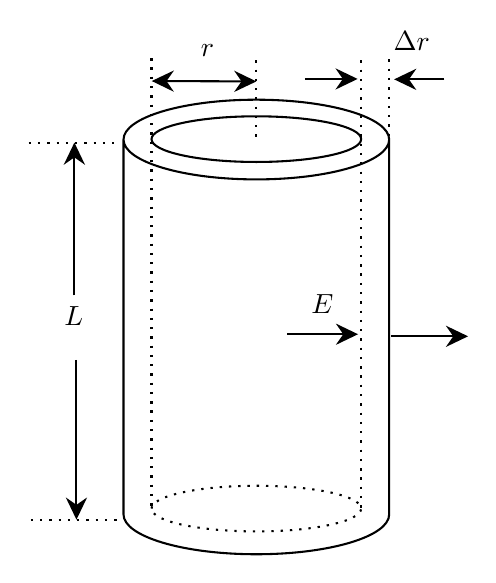
\begin{tikzpicture}[x=0.75pt,y=0.75pt,yscale=-1,xscale=1]
%uncomment if require: \path (0,466); %set diagram left start at 0, and has height of 466

%Shape: Can [id:dp3421118324489345] 
\draw   (363,119.2) -- (363,299.8) .. controls (363,310.4) and (334.35,319) .. (299,319) .. controls (263.65,319) and (235,310.4) .. (235,299.8) -- (235,119.2) .. controls (235,108.6) and (263.65,100) .. (299,100) .. controls (334.35,100) and (363,108.6) .. (363,119.2) .. controls (363,129.8) and (334.35,138.4) .. (299,138.4) .. controls (263.65,138.4) and (235,129.8) .. (235,119.2) ;
%Shape: Ellipse [id:dp6554609238016449] 
\draw   (248.5,119) .. controls (248.5,112.92) and (271.11,108) .. (299,108) .. controls (326.89,108) and (349.5,112.92) .. (349.5,119) .. controls (349.5,125.08) and (326.89,130) .. (299,130) .. controls (271.11,130) and (248.5,125.08) .. (248.5,119) -- cycle ;
%Shape: Ellipse [id:dp4678826933439224] 
\draw  [dash pattern={on 0.84pt off 2.51pt}] (248.5,297) .. controls (248.5,290.92) and (271.11,286) .. (299,286) .. controls (326.89,286) and (349.5,290.92) .. (349.5,297) .. controls (349.5,303.08) and (326.89,308) .. (299,308) .. controls (271.11,308) and (248.5,303.08) .. (248.5,297) -- cycle ;
%Straight Lines [id:da8805055120554433] 
\draw  [dash pattern={on 0.84pt off 2.51pt}]  (248.5,80) -- (248.5,297) ;
%Straight Lines [id:da1519700639364343] 
\draw  [dash pattern={on 0.84pt off 2.51pt}]  (349.5,81) -- (349.5,297) ;
%Straight Lines [id:da859475605792118] 
\draw  [dash pattern={on 0.84pt off 2.51pt}]  (299,81) -- (299,119) ;
%Straight Lines [id:da27539715987896596] 
\draw    (314,213) -- (345,213) ;
\draw [shift={(348,213)}, rotate = 180] [fill={rgb, 255:red, 0; green, 0; blue, 0 }  ][line width=0.08]  [draw opacity=0] (10.72,-5.15) -- (0,0) -- (10.72,5.15) -- (7.12,0) -- cycle    ;
%Straight Lines [id:da18042493663353087] 
\draw    (364,214) -- (398,214) ;
\draw [shift={(401,214)}, rotate = 180] [fill={rgb, 255:red, 0; green, 0; blue, 0 }  ][line width=0.08]  [draw opacity=0] (10.72,-5.15) -- (0,0) -- (10.72,5.15) -- (7.12,0) -- cycle    ;
%Straight Lines [id:da49920586904684927] 
\draw  [dash pattern={on 0.84pt off 2.51pt}]  (189.33,120.67) -- (233.33,120.67) ;
%Straight Lines [id:da1337864117037253] 
\draw  [dash pattern={on 0.84pt off 2.51pt}]  (190.33,302.33) -- (234.33,302.33) ;
%Straight Lines [id:da17401860246007317] 
\draw    (211.33,194.33) -- (211.33,123.67) ;
\draw [shift={(211.33,120.67)}, rotate = 450] [fill={rgb, 255:red, 0; green, 0; blue, 0 }  ][line width=0.08]  [draw opacity=0] (10.72,-5.15) -- (0,0) -- (10.72,5.15) -- (7.12,0) -- cycle    ;
%Straight Lines [id:da6806012790234841] 
\draw    (212.33,225.33) -- (212.33,299.33) ;
\draw [shift={(212.33,302.33)}, rotate = 270] [fill={rgb, 255:red, 0; green, 0; blue, 0 }  ][line width=0.08]  [draw opacity=0] (10.72,-5.15) -- (0,0) -- (10.72,5.15) -- (7.12,0) -- cycle    ;
%Straight Lines [id:da8521846026267319] 
\draw    (251.6,91.01) -- (296,91.19) ;
\draw [shift={(299,91.2)}, rotate = 180.23] [fill={rgb, 255:red, 0; green, 0; blue, 0 }  ][line width=0.08]  [draw opacity=0] (10.72,-5.15) -- (0,0) -- (10.72,5.15) -- (7.12,0) -- cycle    ;
\draw [shift={(248.6,91)}, rotate = 0.23] [fill={rgb, 255:red, 0; green, 0; blue, 0 }  ][line width=0.08]  [draw opacity=0] (10.72,-5.15) -- (0,0) -- (10.72,5.15) -- (7.12,0) -- cycle    ;
%Straight Lines [id:da617352227336923] 
\draw  [dash pattern={on 0.84pt off 2.51pt}]  (363,80.6) -- (363,119.2) ;
%Straight Lines [id:da24251114927538997] 
\draw    (322.4,90) -- (344.8,90) ;
\draw [shift={(347.8,90)}, rotate = 180] [fill={rgb, 255:red, 0; green, 0; blue, 0 }  ][line width=0.08]  [draw opacity=0] (10.72,-5.15) -- (0,0) -- (10.72,5.15) -- (7.12,0) -- cycle    ;
%Straight Lines [id:da16161610058919362] 
\draw    (389.6,90.2) -- (368.4,90.2) ;
\draw [shift={(365.4,90.2)}, rotate = 360] [fill={rgb, 255:red, 0; green, 0; blue, 0 }  ][line width=0.08]  [draw opacity=0] (10.72,-5.15) -- (0,0) -- (10.72,5.15) -- (7.12,0) -- cycle    ;

% Text Node
\draw (324,192.4) node [anchor=north west][inner sep=0.75pt]    {$E$};
% Text Node
\draw (205,198.4) node [anchor=north west][inner sep=0.75pt]    {$L$};
% Text Node
\draw (270.8,71.8) node [anchor=north west][inner sep=0.75pt]    {$r$};
% Text Node
\draw (363.6,65.8) node [anchor=north west][inner sep=0.75pt]    {$\Delta r$};


\end{tikzpicture}

\end{center}
Sử dụng định luật Gauss có thể tìm được mật độ điện tích bên trong hình trụ. Xét vỏ hình trụ mỏng như hình, gọi $\rho(r)$ là mật độ điện tích ở điểm cách trục một khoảng $r$. Một dòng điện có cường độ $ 2\pi rLE(r)$ đi vào vỏ và một dòng điện có cường độ $ 2\pi\left(r+\Delta r\right)LE\left(r+\Delta r\right)$ đi ra khỏi nó.\\
Theo định luật Gauss:
$$ K\left(r+\Delta r\right)2\pi\left(r+\Delta r\right)L-Kr2\pi rL=\dfrac{1}{\varepsilon_0}\rho 2\pi r\Delta rL.$$
Từ đó chúng ta tìm được:
$$\rho=\dfrac{2\varepsilon_0\omega m}{e}\left(\omega\pm\dfrac{eB}{m}\right).$$
Lưu ý rằng, mật độ điện tích trong hình trụ không phụ thuộc vào $r$.\\
Mật độ có thể dương, âm hoặc bằng không - tùy thuộc vào hướng và độ lớn của từ trường và vận tốc góc. Mật độ sẽ bằng không nếu $\omega=\dfrac{|e|B}{m}$. Đối với trường hợp này, các điện tích dương và âm không được tách ra bên trong hình trụ bởi vì lực hướng tâm được cung cấp bởi hiệu ứng Lorentz chỉ là những gì cần thiết để duy trì chuyển động tròn.\\
Ghi chú: Để hình dung về độ lớn của vận tốc góc, giả sử rằng từ trường có giá trị tương đối so với từ trường Trái Đất ở gần Xích Đạo, tức là $ B=3\times{10^{-5}}\ \mathrm{T}$. Mật độ điện tích bằng $0$ tương ứng với vận tốc góc $\omega=\dfrac{eB}{m}=5.3\times{10^6}\ \mathrm{s^{-1}},$ tức là hơn 50 triệu vòng quay mỗi phút! Sự quay vòng nhanh như vậy không thể xảy ra trong thực tế, vì không một vật liệu nào có thể chịu được.
\end{loigiai}


\begin{vd}[Khúc xạ điện từ]
Cho một nguồn ${S}$ phát ra các electron có tốc độ bằng nhau và bằng $v_{0}$. Các electron được cho bay qua một vùng điện trường hẹp có bề rộng $d$. Nguồn phát nằm cách biên của vùng một khoảng là ${L} \ ({L} \gg {d})$. Chọn hệ quy chiếu như hình vẽ. Khối lượng và điện tích của electron lần lượt là
${m}$ và ${q}_{{e}}=-{e}$. Bỏ qua tương tác giữa các electron và tác dụng của trọng lực. 
\\
\textit{Lưu ý: Các ý $1)$ và $2)$ sau đây là hai bài toán độc lập, không liên quan tới nhau.}
\begin{center}
\tikzset{every picture/.style={line width=0.75pt}} %set default line width to 0.75pt        

\begin{tikzpicture}[x=0.75pt,y=0.75pt,yscale=-0.8,xscale=0.8]
%uncomment if require: \path (0,366); %set diagram left start at 0, and has height of 366

%Straight Lines [id:da46697420421082536] 
\draw [line width=1.5]    (118,178) -- (448,178) ;
\draw [shift={(452,178)}, rotate = 180] [fill={rgb, 255:red, 0; green, 0; blue, 0 }  ][line width=0.08]  [draw opacity=0] (11.61,-5.58) -- (0,0) -- (11.61,5.58) -- cycle    ;
%Straight Lines [id:da2506014250640798] 
\draw [line width=1.5]    (294,271) -- (294,55) ;
\draw [shift={(294,51)}, rotate = 450] [fill={rgb, 255:red, 0; green, 0; blue, 0 }  ][line width=0.08]  [draw opacity=0] (11.61,-5.58) -- (0,0) -- (11.61,5.58) -- cycle    ;
%Shape: Circle [id:dp8603477382918159] 
\draw  [fill={rgb, 255:red, 74; green, 74; blue, 74 }  ,fill opacity=1 ] (291,178) .. controls (291,176.34) and (292.34,175) .. (294,175) .. controls (295.66,175) and (297,176.34) .. (297,178) .. controls (297,179.66) and (295.66,181) .. (294,181) .. controls (292.34,181) and (291,179.66) .. (291,178) -- cycle ;
%Straight Lines [id:da25133620030654247] 
\draw    (177,193) -- (291,193) ;
\draw [shift={(294,193)}, rotate = 180] [fill={rgb, 255:red, 0; green, 0; blue, 0 }  ][line width=0.08]  [draw opacity=0] (10.72,-5.15) -- (0,0) -- (10.72,5.15) -- (7.12,0) -- cycle    ;
\draw [shift={(174,193)}, rotate = 0] [fill={rgb, 255:red, 0; green, 0; blue, 0 }  ][line width=0.08]  [draw opacity=0] (10.72,-5.15) -- (0,0) -- (10.72,5.15) -- (7.12,0) -- cycle    ;
%Straight Lines [id:da47174237886153136] 
\draw    (316,59) -- (316,269) ;
%Shape: Circle [id:dp9866667209894922] 
\draw  [fill={rgb, 255:red, 74; green, 74; blue, 74 }  ,fill opacity=1 ] (173,178) .. controls (173,176.34) and (174.34,175) .. (176,175) .. controls (177.66,175) and (179,176.34) .. (179,178) .. controls (179,179.66) and (177.66,181) .. (176,181) .. controls (174.34,181) and (173,179.66) .. (173,178) -- cycle ;
%Straight Lines [id:da8255306861089213] 
\draw    (366,77) -- (307.23,129.99) ;
\draw [shift={(305,132)}, rotate = 317.96000000000004] [fill={rgb, 255:red, 0; green, 0; blue, 0 }  ][line width=0.08]  [draw opacity=0] (10.72,-5.15) -- (0,0) -- (10.72,5.15) -- (7.12,0) -- cycle    ;
%Straight Lines [id:da4989388686161913] 
\draw    (244,244) -- (290,244) ;
\draw [shift={(292,244)}, rotate = 180] [fill={rgb, 255:red, 0; green, 0; blue, 0 }  ][line width=0.08]  [draw opacity=0] (12,-3) -- (0,0) -- (12,3) -- cycle    ;
%Straight Lines [id:da14163511506448256] 
\draw    (358,245) -- (318,245) ;
\draw [shift={(316,245)}, rotate = 360] [fill={rgb, 255:red, 0; green, 0; blue, 0 }  ][line width=0.08]  [draw opacity=0] (12,-3) -- (0,0) -- (12,3) -- cycle    ;

% Text Node
\draw (157,157.4) node [anchor=north west][inner sep=0.75pt]    {$S$};
% Text Node
\draw (275,158.4) node [anchor=north west][inner sep=0.75pt]    {$O$};
% Text Node
\draw (227,155.4) node [anchor=north west][inner sep=0.75pt]    {$L$};
% Text Node
\draw (346,56) node [anchor=north west][inner sep=0.75pt]   [align=left] {Vùng điện trường};
% Text Node
\draw (275,47.4) node [anchor=north west][inner sep=0.75pt]    {$y$};
% Text Node
\draw (442,181.4) node [anchor=north west][inner sep=0.75pt]    {$x$};
% Text Node
\draw (299,241.4) node [anchor=north west][inner sep=0.75pt]    {$d$};
\end{tikzpicture}
\end{center}

\begin{enumerate}[1)]
    \item Điện trường được tạo ra bởi một hệ điện tích phân bố theo một quy luật xác định. Bỏ qua thành phần điện trường ${E}_{{x}}$. Sau khi các electron bay qua vùng điện trường, chúng chuyển động theo phương song song với trục ${Ox}$. Tìm biểu thức mật độ điện khối của vùng điện trường tại vị trí có tọa độ ${y}$.
    \item Điện trường được tạo ra nhờ hai lưới kim loại đặt vuông góc với trục ${Ox}$, được nối vào hiệu điện thế $U$ không đổi. Gọi $i$ và $r$ lần lượt là góc hợp giữa phương của electron đi tới và của electron rời khỏi vùng từ trường với phương của trục ${Ox}$.
\begin{enumerate}[a)]
    \item Tìm tỉ số $\dfrac{\sin i}{\sin r}$.
    \item Các electron ló ra khỏi điện trường trong vùng lân cận, khá gần với trục $Ox$ giống như được phát ra từ ``ảnh'' ${S}^{\prime}$ của nguồn ${S}$. Tìm vị trí của ${S}^{\prime}$.
\end{enumerate}
\end{enumerate}
\end{vd}


\begin{loigiai}
\begin{enumerate}[1)]
    \item Xét tia tới vùng điện trường với góc tới $\varphi$. Bỏ qua thành phần điện trường ${E}_{{x}}$, chỉ tính đến thành phần ${E}_{{y}}$ coi là không đổi khi e bay qua vùng.\\
Thời gian bay qua vùng: $t=\dfrac{d}{v \cos \varphi}$.\\
Cường độ điện trường ${E}_{{y}}$ của vùng hướng theo chiều ra xa ${O}$ và:
\[a=\dfrac{E e}{m}=\dfrac{v \sin \varphi}{t},\]
\[\begin{aligned} 
\Rightarrow E&=\dfrac{m v^{2} \sin \varphi \cdot \cos \varphi}{e d}\\
&=\dfrac{m v^{2}}{e d} \dfrac{y L}{y^{2}+L^{2}} \approx \dfrac{m v^{2}}{e d L} y.
\end{aligned}\]
Ta có:
\begin{align*}
\rho&=-\varepsilon_0\dfrac{\mathrm{d} E}{\mathrm{d} y}=-\varepsilon_0\dfrac{m v^{2}}{e d} \dfrac{L\left(y^{2}+L^{2}\right)-y L .2 y}{\left(y^{2}+L^{2}\right)^{2}}\\
&=-\varepsilon_0\dfrac{m v^{2}}{e d} \dfrac{L\left(L^{2}-y^{2}\right)}{\left(y^{2}+L^{2}\right)^{2}} \approx-\varepsilon_0\dfrac{m v^{2}}{e d L}\left(1-3 \dfrac{y^{2}}{L^{2}}\right).
\end{align*}
\item Điện trường giữa hai lưới kim loại (đóng vai trò là các bản tụ phẳng) là đều và hướng theo trục $x$ nên thành phần $v_{y}$ của e khi qua vùng là không đổi. 
\begin{enumerate}[a)]
    \item Ta có: $\dfrac{\sin i}{\sin r}=\dfrac{v_{y}}{v} \cdot \dfrac{v^{\prime}}{v_{y}}=\dfrac{v^{\prime}}{v}$.\\
Mà: 
\[\dfrac{1}{2} m v^{2} \pm e U=\dfrac{1}{2} m v^{\prime 2},\] 
(dấu của $eU$ phụ thuộc vào chiều của hiệu điện thế). Vậy:
\[
\dfrac{\sin i}{\sin r}=\sqrt{1 \pm \dfrac{2 e U}{m v^{2}}}.
\]
\item Ta đi tính cho trường hợp góc ${i}$ và ${r}$ đều khá nhỏ, bỏ qua độ rộng ${d}$ của vùng điện trường và độ lệch $\Delta {y}$ của tia vào và tia ló ra khi chuyển động của vùng điện trường.
Vậy:
\[\dfrac{\sin i}{\sin r} \approx \dfrac{\tan i}{\tan r}=\dfrac{y}{L} \cdot \dfrac{-L^{\prime}}{y}=-\dfrac{L^{\prime}}{L}.\]
\[\rt L^{\prime}=-L \sqrt{1 \pm \dfrac{2 e U}{m v^{2}}}.\]
\end{enumerate} 
\end{enumerate}
\end{loigiai}

\begin{vd}[Hệ vỏ cầu nối đất]
\begin{enumerate}[1)]
    \item Trên hình $(a)$, hai vỏ cầu kim loại đặt đồng tâm có các bán kính $a$ và $c$ được nối đất. Đưa vào giữa hai bản một điện tích $q$ nằm cách tâm hai vỏ cầu một khoảng $b$ $(a<b<c)$. Tìm điện tích $q_0$ và $Q_0$ trên các vỏ cầu.
\begin{center}
\tikzset{every picture/.style={line width=0.75pt}} %set default line width to 0.75pt        

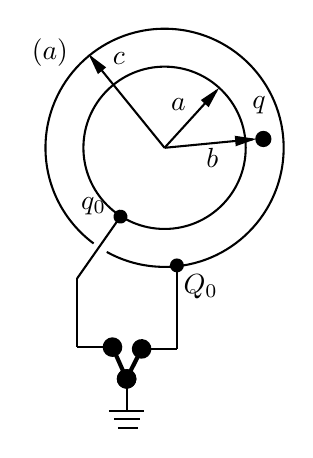
\begin{tikzpicture}[x=0.75pt,y=0.75pt,yscale=-0.85,xscale=0.85]
%uncomment if require: \path (0,300); %set diagram left start at 0, and has height of 300

%Shape: Circle [id:dp7235414025348001] 
\draw   (223,118) .. controls (223,92.59) and (243.59,72) .. (269,72) .. controls (294.41,72) and (315,92.59) .. (315,118) .. controls (315,143.41) and (294.41,164) .. (269,164) .. controls (243.59,164) and (223,143.41) .. (223,118) -- cycle ;
%Shape: Circle [id:dp3376765398979207] 
\draw  [fill={rgb, 255:red, 0; green, 0; blue, 0 }  ,fill opacity=1 ] (321,113) .. controls (321,110.79) and (322.79,109) .. (325,109) .. controls (327.21,109) and (329,110.79) .. (329,113) .. controls (329,115.21) and (327.21,117) .. (325,117) .. controls (322.79,117) and (321,115.21) .. (321,113) -- cycle ;
%Straight Lines [id:da3617289603147187] 
\draw    (269,118) -- (319.01,113.19) ;
\draw [shift={(321,113)}, rotate = 534.51] [fill={rgb, 255:red, 0; green, 0; blue, 0 }  ][line width=0.08]  [draw opacity=0] (12,-3) -- (0,0) -- (12,3) -- cycle    ;
%Straight Lines [id:da3095417846990314] 
\draw    (269,118) -- (227.26,66.55) ;
\draw [shift={(226,65)}, rotate = 410.95] [fill={rgb, 255:red, 0; green, 0; blue, 0 }  ][line width=0.08]  [draw opacity=0] (12,-3) -- (0,0) -- (12,3) -- cycle    ;
%Straight Lines [id:da6573278911493619] 
\draw    (269,118) -- (298.5,85.57) ;
\draw [shift={(299.84,84.09)}, rotate = 492.29] [fill={rgb, 255:red, 0; green, 0; blue, 0 }  ][line width=0.08]  [draw opacity=0] (12,-3) -- (0,0) -- (12,3) -- cycle    ;
%Shape: Arc [id:dp5758550915786248] 
\draw  [draw opacity=0] (228.78,172.21) .. controls (212.23,159.91) and (201.5,140.21) .. (201.5,118) .. controls (201.5,80.72) and (231.72,50.5) .. (269,50.5) .. controls (306.28,50.5) and (336.5,80.72) .. (336.5,118) .. controls (336.5,155.28) and (306.28,185.5) .. (269,185.5) .. controls (257.11,185.5) and (245.93,182.42) .. (236.23,177.02) -- (269,118) -- cycle ; \draw   (228.78,172.21) .. controls (212.23,159.91) and (201.5,140.21) .. (201.5,118) .. controls (201.5,80.72) and (231.72,50.5) .. (269,50.5) .. controls (306.28,50.5) and (336.5,80.72) .. (336.5,118) .. controls (336.5,155.28) and (306.28,185.5) .. (269,185.5) .. controls (257.11,185.5) and (245.93,182.42) .. (236.23,177.02) ;
%Straight Lines [id:da6760394888349934] 
\draw    (244,157) -- (219.48,191.98) ;
\draw [shift={(244,157)}, rotate = 125.04] [color={rgb, 255:red, 0; green, 0; blue, 0 }  ][fill={rgb, 255:red, 0; green, 0; blue, 0 }  ][line width=0.75]      (0, 0) circle [x radius= 3.35, y radius= 3.35]   ;
%Straight Lines [id:da52386780794706] 
\draw    (219.48,191.98) -- (219.48,230.98) ;
%Straight Lines [id:da3258652576669081] 
\draw    (276,184.66) -- (276,231.98) ;
\draw [shift={(276,184.66)}, rotate = 90] [color={rgb, 255:red, 0; green, 0; blue, 0 }  ][fill={rgb, 255:red, 0; green, 0; blue, 0 }  ][line width=0.75]      (0, 0) circle [x radius= 3.35, y radius= 3.35]   ;
%Straight Lines [id:da887969340720195] 
\draw    (219.48,230.98) -- (239.48,230.98) ;
%Straight Lines [id:da4878374869102087] 
\draw    (256,231.98) -- (276,231.98) ;
%Straight Lines [id:da39424160833392785] 
\draw [line width=1.5]    (239.48,230.98) -- (247.48,248.98) ;
\draw [shift={(247.48,248.98)}, rotate = 66.04] [color={rgb, 255:red, 0; green, 0; blue, 0 }  ][fill={rgb, 255:red, 0; green, 0; blue, 0 }  ][line width=1.5]      (0, 0) circle [x radius= 4.36, y radius= 4.36]   ;
\draw [shift={(239.48,230.98)}, rotate = 66.04] [color={rgb, 255:red, 0; green, 0; blue, 0 }  ][fill={rgb, 255:red, 0; green, 0; blue, 0 }  ][line width=1.5]      (0, 0) circle [x radius= 4.36, y radius= 4.36]   ;
%Straight Lines [id:da8801959493880728] 
\draw [line width=1.5]    (256,231.98) -- (247.48,248.98) ;
\draw [shift={(247.48,248.98)}, rotate = 116.63] [color={rgb, 255:red, 0; green, 0; blue, 0 }  ][fill={rgb, 255:red, 0; green, 0; blue, 0 }  ][line width=1.5]      (0, 0) circle [x radius= 4.36, y radius= 4.36]   ;
\draw [shift={(256,231.98)}, rotate = 116.63] [color={rgb, 255:red, 0; green, 0; blue, 0 }  ][fill={rgb, 255:red, 0; green, 0; blue, 0 }  ][line width=1.5]      (0, 0) circle [x radius= 4.36, y radius= 4.36]   ;
%Straight Lines [id:da5134627984646966] 
\draw    (247.48,248.98) -- (247.48,266.66) ;
%Straight Lines [id:da5979824414798764] 
\draw    (237.48,266.98) -- (257.48,266.98) ;
%Straight Lines [id:da18769168360442912] 
\draw    (240.48,271.98) -- (254.93,271.98) ;
%Straight Lines [id:da2654621554389449] 
\draw    (242.48,277) -- (253.93,277) ;

% Text Node
\draw (271,88.4) node [anchor=north west][inner sep=0.75pt]    {$a$};
% Text Node
\draw (291,116.4) node [anchor=north west][inner sep=0.75pt]    {$b$};
% Text Node
\draw (238,62.4) node [anchor=north west][inner sep=0.75pt]    {$c$};
% Text Node
\draw (317,87.4) node [anchor=north west][inner sep=0.75pt]    {$q$};
% Text Node
\draw (220,144.4) node [anchor=north west][inner sep=0.75pt]    {$q_{0}$};
% Text Node
\draw (278,188.06) node [anchor=north west][inner sep=0.75pt]    {$Q_{0}$};
% Text Node
\draw (192,54.4) node [anchor=north west][inner sep=0.75pt]    {$( a)$};
\end{tikzpicture}
\end{center}
\item Bây giờ ngắt khóa cho cả hai vỏ cầu đều không tiếp đất rồi di chuyển điện tích $q$ ra xa vô cùng. Dùng một khóa đôi lần lượt tiếp đất cho vỏ cầu trong, rồi vỏ cầu ngoài, rồi lại vỏ cầu trong, cứ lần lượt như thế sau khi mỗi vỏ cầu (trong và ngoài) tiếp đất $n$ lần, điện tích trên chúng là $q_n$ và $Q_n$. Tìm các điện tích này.
\begin{center}
\tikzset{every picture/.style={line width=0.75pt}} %set default line width to 0.75pt        

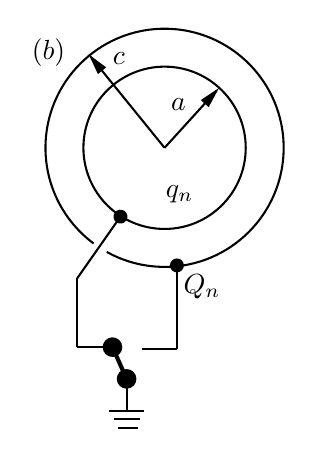
\begin{tikzpicture}[x=0.75pt,y=0.75pt,yscale=-0.85,xscale=0.85]
%uncomment if require: \path (0,300); %set diagram left start at 0, and has height of 300

%Shape: Circle [id:dp7235414025348001] 
\draw   (223,118) .. controls (223,92.59) and (243.59,72) .. (269,72) .. controls (294.41,72) and (315,92.59) .. (315,118) .. controls (315,143.41) and (294.41,164) .. (269,164) .. controls (243.59,164) and (223,143.41) .. (223,118) -- cycle ;
%Straight Lines [id:da3095417846990314] 
\draw    (269,118) -- (227.26,66.55) ;
\draw [shift={(226,65)}, rotate = 410.95] [fill={rgb, 255:red, 0; green, 0; blue, 0 }  ][line width=0.08]  [draw opacity=0] (12,-3) -- (0,0) -- (12,3) -- cycle    ;
%Straight Lines [id:da6573278911493619] 
\draw    (269,118) -- (298.5,85.57) ;
\draw [shift={(299.84,84.09)}, rotate = 492.29] [fill={rgb, 255:red, 0; green, 0; blue, 0 }  ][line width=0.08]  [draw opacity=0] (12,-3) -- (0,0) -- (12,3) -- cycle    ;
%Shape: Arc [id:dp5758550915786248] 
\draw  [draw opacity=0] (228.78,172.21) .. controls (212.23,159.91) and (201.5,140.21) .. (201.5,118) .. controls (201.5,80.72) and (231.72,50.5) .. (269,50.5) .. controls (306.28,50.5) and (336.5,80.72) .. (336.5,118) .. controls (336.5,155.28) and (306.28,185.5) .. (269,185.5) .. controls (257.11,185.5) and (245.93,182.42) .. (236.23,177.02) -- (269,118) -- cycle ; \draw   (228.78,172.21) .. controls (212.23,159.91) and (201.5,140.21) .. (201.5,118) .. controls (201.5,80.72) and (231.72,50.5) .. (269,50.5) .. controls (306.28,50.5) and (336.5,80.72) .. (336.5,118) .. controls (336.5,155.28) and (306.28,185.5) .. (269,185.5) .. controls (257.11,185.5) and (245.93,182.42) .. (236.23,177.02) ;
%Straight Lines [id:da6760394888349934] 
\draw    (244,157) -- (219.48,191.98) ;
\draw [shift={(244,157)}, rotate = 125.04] [color={rgb, 255:red, 0; green, 0; blue, 0 }  ][fill={rgb, 255:red, 0; green, 0; blue, 0 }  ][line width=0.75]      (0, 0) circle [x radius= 3.35, y radius= 3.35]   ;
%Straight Lines [id:da52386780794706] 
\draw    (219.48,191.98) -- (219.48,230.98) ;
%Straight Lines [id:da3258652576669081] 
\draw    (276,184.66) -- (276,231.98) ;
\draw [shift={(276,184.66)}, rotate = 90] [color={rgb, 255:red, 0; green, 0; blue, 0 }  ][fill={rgb, 255:red, 0; green, 0; blue, 0 }  ][line width=0.75]      (0, 0) circle [x radius= 3.35, y radius= 3.35]   ;
%Straight Lines [id:da887969340720195] 
\draw    (219.48,230.98) -- (239.48,230.98) ;
%Straight Lines [id:da4878374869102087] 
\draw    (256,231.98) -- (276,231.98) ;
%Straight Lines [id:da39424160833392785] 
\draw [line width=1.5]    (239.48,230.98) -- (247.48,248.98) ;
\draw [shift={(247.48,248.98)}, rotate = 66.04] [color={rgb, 255:red, 0; green, 0; blue, 0 }  ][fill={rgb, 255:red, 0; green, 0; blue, 0 }  ][line width=1.5]      (0, 0) circle [x radius= 4.36, y radius= 4.36]   ;
\draw [shift={(239.48,230.98)}, rotate = 66.04] [color={rgb, 255:red, 0; green, 0; blue, 0 }  ][fill={rgb, 255:red, 0; green, 0; blue, 0 }  ][line width=1.5]      (0, 0) circle [x radius= 4.36, y radius= 4.36]   ;
%Straight Lines [id:da5134627984646966] 
\draw    (247.48,248.98) -- (247.48,266.66) ;
%Straight Lines [id:da5979824414798764] 
\draw    (237.48,266.98) -- (257.48,266.98) ;
%Straight Lines [id:da18769168360442912] 
\draw    (240.48,271.98) -- (254.93,271.98) ;
%Straight Lines [id:da2654621554389449] 
\draw    (242.48,277) -- (253.93,277) ;

% Text Node
\draw (271,88.4) node [anchor=north west][inner sep=0.75pt]    {$a$};
% Text Node
\draw (238,62.4) node [anchor=north west][inner sep=0.75pt]    {$c$};
% Text Node
\draw (268,137.4) node [anchor=north west][inner sep=0.75pt]    {$q_{n}$};
% Text Node
\draw (278,188.06) node [anchor=north west][inner sep=0.75pt]    {$Q_{n}$};
% Text Node
\draw (192,54.4) node [anchor=north west][inner sep=0.75pt]    {$( b)$};
\end{tikzpicture}
\end{center}
\end{enumerate}
\end{vd}


\begin{loigiai}
\begin{enumerate}[1)]
    \item Điện thế vỏ cầu ngoài bằng không nên điện trường bên ngoài hệ cũng bằng không. Do đó tổng điện tích của hệ phải bằng không theo định luật Gauss:
    \[
q+q_{0}+Q_{0}=0. \tag{1} \label{loz1}
\]
Xét điện thế tại tâm của hệ, nó được chồng chất từ 3 hệ điện tích $q$, $q_0$, $Q_0$ và điện thế đó cũng bằng không:
\[
\dfrac{q}{4 \pi \varepsilon_{0} b}+\dfrac{q_{0}}{4 \pi \varepsilon_{0} a}+\dfrac{Q_{0}}{4 \pi \varepsilon_{0} c}=0. \tag{2} \label{loz2}
\]
Giải hệ phương trình (\ref{loz1}) và (\ref{loz2}) ta được:
$$
q_{0}=-q \dfrac{a}{b} \dfrac{c-b}{c-a} \  \text { và } \ Q_{0}=-q \dfrac{c}{b} \dfrac{b-a}{c-a}.
$$
\item Sau khi nối đất lần đầu vào vỏ cầu trong, điện tích trên vỏ cầu lớn vẫn là $Q_0$, còn vỏ trong có điện tích mới $q_1$ sao cho điện thế của nó bằng không:
$$
\dfrac{q_{1}}{4 \pi \varepsilon_{0} a}+\dfrac{Q_{0}}{4 \pi \varepsilon_{0} c}=0.
$$
Suy ra: $q_1=-Q_0\dfrac{a}{c}$.
Tương tự như vậy sau khi nối vỏ cầu ngoài với đất lần thứ nhất:
$$
\dfrac{q_{1}}{4 \pi \varepsilon_{0} c}+\dfrac{Q_{1}}{4 \pi \varepsilon_{0} c}=0 \Rightarrow  Q_{1}=-q_{1}=Q_{0} \dfrac{a}{c}.
$$
Dễ thấy sau lần thứ hai, điện tích trên vỏ cầu nhỏ sẽ là:
\[\begin{aligned}  
\dfrac{q_{2}}{4 \pi \varepsilon_{0} a}+\dfrac{Q_{1}}{4 \pi \varepsilon_{0} c} &= 0 \Rightarrow q_{2} = -Q_{1} \dfrac{a}{c}=-Q_{0}\left(\dfrac{a}{c}\right)^{2}, \\
\dfrac{q_{2}}{4 \pi \varepsilon_{0} c}+\dfrac{Q_{2}}{4 \pi \varepsilon_{0} c} &= 0 \Rightarrow  Q_{2} = -q_{2}=Q_{0}\left(\dfrac{a}{c}\right)^{2}.
\end{aligned}\]

Vậy sau $n$ lần tiếp đất lần lượt kết quả thu được:
$$
q_{n}=-Q_{0}\left(\dfrac{a}{c}\right)^{n}=q \dfrac{c}{b} \dfrac{b-a}{c-a}\left(\dfrac{a}{c}\right)^{n} \text { và } Q_{n}=-q_{n}.
$$
\end{enumerate}
\end{loigiai}


\begin{vd}[Điện thế của tam giác vuông]
    Cho tấm phẳng $ABC$ hình tam giác vuông ($AB=5s$, $AC=12s$ và $BC=13s$) với mật độ điện mặt $\sigma$. $D$ là trung điểm của cạnh $BC$. Chúng ta kí hiệu điện thế của điểm $P$ là $\phi(P)$. Điện thế tại vô cùng là không. Cho: \[\phi(B)+\phi(C)+\phi(D)=\dfrac{k\sigma s}{\varepsilon_0},\] 
    với $k$ là một hằng số không thứ nguyên. Hãy xác định giá trị của $k$. 
\end{vd}
\begin{loigiai}\\
Nếu ta ghép hai tam giác như trên lại với nhau, ta sẽ có một hình chữ nhật có kích thước hai cạnh lần lượt là $5s$ và $12s$. Gọi điện thế tại tâm của hình chữ nhật này là $V$. Theo nguyên lý chồng chất của điện thế, ta suy ra $\phi(D)=\dfrac{V}{2}$. 
\begin{center}
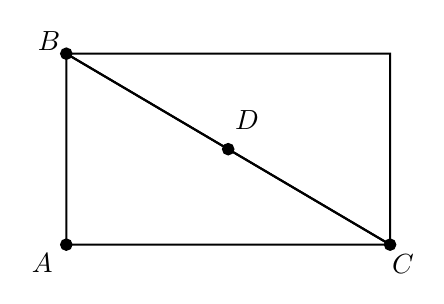
\begin{tikzpicture}[x=0.75pt,y=0.75pt,yscale=-1,xscale=1]
%uncomment if require: \path (0,146); %set diagram left start at 0, and has height of 146

%Shape: Right Triangle [id:dp7856288760770522] 
\draw   (270.71,23.03) -- (426.71,115.03) -- (270.71,115.03) -- cycle ;
%Shape: Circle [id:dp5020636092733206] 
\draw  [fill={rgb, 255:red, 0; green, 0; blue, 0 }  ,fill opacity=1 ] (268.19,23.03) .. controls (268.19,21.64) and (269.32,20.52) .. (270.71,20.52) .. controls (272.1,20.52) and (273.22,21.64) .. (273.22,23.03) .. controls (273.22,24.42) and (272.1,25.55) .. (270.71,25.55) .. controls (269.32,25.55) and (268.19,24.42) .. (268.19,23.03) -- cycle ;
%Shape: Circle [id:dp8576118434240458] 
\draw  [fill={rgb, 255:red, 0; green, 0; blue, 0 }  ,fill opacity=1 ] (346.19,69.03) .. controls (346.19,67.64) and (347.32,66.52) .. (348.71,66.52) .. controls (350.1,66.52) and (351.22,67.64) .. (351.22,69.03) .. controls (351.22,70.42) and (350.1,71.55) .. (348.71,71.55) .. controls (347.32,71.55) and (346.19,70.42) .. (346.19,69.03) -- cycle ;
%Shape: Circle [id:dp725015984181985] 
\draw  [fill={rgb, 255:red, 0; green, 0; blue, 0 }  ,fill opacity=1 ] (424.19,115.03) .. controls (424.19,113.64) and (425.32,112.52) .. (426.71,112.52) .. controls (428.1,112.52) and (429.22,113.64) .. (429.22,115.03) .. controls (429.22,116.42) and (428.1,117.55) .. (426.71,117.55) .. controls (425.32,117.55) and (424.19,116.42) .. (424.19,115.03) -- cycle ;
%Shape: Right Triangle [id:dp7437109781698188] 
\draw   (426.71,115.03) -- (270.71,23.03) -- (426.71,23.03) -- cycle ;
%Shape: Circle [id:dp9482880599050558] 
\draw  [fill={rgb, 255:red, 0; green, 0; blue, 0 }  ,fill opacity=1 ] (268.19,115.03) .. controls (268.19,113.64) and (269.32,112.52) .. (270.71,112.52) .. controls (272.1,112.52) and (273.22,113.64) .. (273.22,115.03) .. controls (273.22,116.42) and (272.1,117.55) .. (270.71,117.55) .. controls (269.32,117.55) and (268.19,116.42) .. (268.19,115.03) -- cycle ;

% Text Node
\draw (252.6,118.08) node [anchor=north west][inner sep=0.75pt]    {$A$};
% Text Node
\draw (255.52,11) node [anchor=north west][inner sep=0.75pt]    {$B$};
% Text Node
\draw (426.19,118.43) node [anchor=north west][inner sep=0.75pt]    {$C$};
% Text Node
\draw (350.52,48.93) node [anchor=north west][inner sep=0.75pt]    {$D$};
\end{tikzpicture}
\end{center}

Bây giờ ta xét điện thế tại một góc của hình chữ nhật. Điện thế tại đây là $\phi(B) + \phi(C)$. Nếu như ta ghép bốn hình chữ nhật như trên lại với nhau để tạo thành một hình chữ nhật khác có các cạnh là $10s$ và $24s$, điện thế tại tâm hình chữ nhật này sẽ là $2V$.
\begin{center}
        
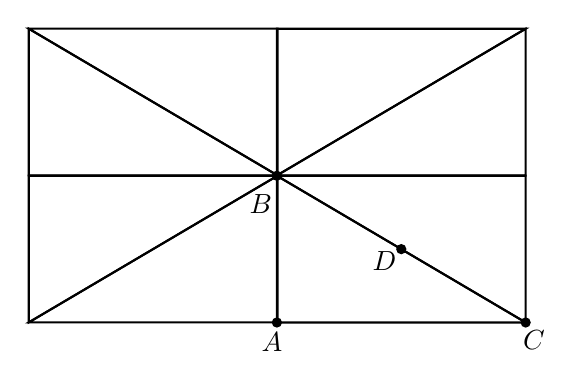
\begin{tikzpicture}[x=0.75pt,y=0.75pt,yscale=-1,xscale=1]
%uncomment if require: \path (0,188); %set diagram left start at 0, and has height of 188

%Shape: Right Triangle [id:dp6040990867089013] 
\draw   (464.7,16.2) -- (344.84,86.88) -- (464.7,86.88) -- cycle ;
%Shape: Right Triangle [id:dp8423695954755102] 
\draw   (344.84,86.88) -- (464.7,16.2) -- (344.84,16.2) -- cycle ;
%Shape: Right Triangle [id:dp30632792257472374] 
\draw   (464.73,157.71) -- (344.86,87.02) -- (464.73,87.02) -- cycle ;
%Shape: Right Triangle [id:dp9613549485070378] 
\draw   (344.86,87.02) -- (464.73,157.71) -- (344.86,157.71) -- cycle ;


%Shape: Right Triangle [id:dp04741643312830357] 
\draw   (225.33,16.17) -- (345.19,86.85) -- (225.33,86.85) -- cycle ;
%Shape: Right Triangle [id:dp5952677937142539] 
\draw   (345.19,86.85) -- (225.33,16.17) -- (345.19,16.17) -- cycle ;
%Shape: Right Triangle [id:dp5720905002999583] 
\draw   (225.3,157.68) -- (345.17,87) -- (225.3,87) -- cycle ;
%Shape: Right Triangle [id:dp13845149125527412] 
\draw   (345.17,87) -- (225.3,157.68) -- (345.17,157.68) -- cycle ;



%Shape: Ellipse [id:dp5881915630437773] 
\draw  [fill={rgb, 255:red, 0; green, 0; blue, 0 }  ,fill opacity=1 ] (342.93,157.71) .. controls (342.93,156.64) and (343.8,155.78) .. (344.86,155.78) .. controls (345.93,155.78) and (346.8,156.64) .. (346.8,157.71) .. controls (346.8,158.78) and (345.93,159.65) .. (344.86,159.65) .. controls (343.8,159.65) and (342.93,158.78) .. (342.93,157.71) -- cycle ;
%Shape: Ellipse [id:dp08796214303835082] 
\draw  [fill={rgb, 255:red, 0; green, 0; blue, 0 }  ,fill opacity=1 ] (402.86,122.37) .. controls (402.86,121.3) and (403.73,120.43) .. (404.8,120.43) .. controls (405.86,120.43) and (406.73,121.3) .. (406.73,122.37) .. controls (406.73,123.44) and (405.86,124.3) .. (404.8,124.3) .. controls (403.73,124.3) and (402.86,123.44) .. (402.86,122.37) -- cycle ;
%Shape: Ellipse [id:dp10230262305383064] 
\draw  [fill={rgb, 255:red, 0; green, 0; blue, 0 }  ,fill opacity=1 ] (462.79,157.71) .. controls (462.79,156.64) and (463.66,155.78) .. (464.73,155.78) .. controls (465.8,155.78) and (466.66,156.64) .. (466.66,157.71) .. controls (466.66,158.78) and (465.8,159.65) .. (464.73,159.65) .. controls (463.66,159.65) and (462.79,158.78) .. (462.79,157.71) -- cycle ;
%Shape: Ellipse [id:dp40506570554551313] 
\draw  [fill={rgb, 255:red, 0; green, 0; blue, 0 }  ,fill opacity=1 ] (342.93,87.02) .. controls (342.93,85.96) and (343.8,85.09) .. (344.86,85.09) .. controls (345.93,85.09) and (346.8,85.96) .. (346.8,87.02) .. controls (346.8,88.09) and (345.93,88.96) .. (344.86,88.96) .. controls (343.8,88.96) and (342.93,88.09) .. (342.93,87.02) -- cycle ;


% Text Node
\draw (336.07,161.25) node [anchor=north west][inner sep=0.75pt]    {$A$};
% Text Node
\draw (330.28,94.71) node [anchor=north west][inner sep=0.75pt]    {$B$};
% Text Node
\draw (462.02,160.26) node [anchor=north west][inner sep=0.75pt]    {$C$};
% Text Node
\draw (389.54,122.05) node [anchor=north west][inner sep=0.75pt]    {$D$};


\end{tikzpicture}
\end{center}
Từ đó suy ra:
\begin{equation*}
        4\tron{\phi(B) + \phi(C)} = 2V
        \Leftrightarrow \phi(B)+\phi(C)=\dfrac{V}{2}.
\end{equation*}
Vậy $\phi(D)+\phi(B)+\phi(C)=V$, ta sẽ đi tính điện thế $V$.\\
Xét một tam giác cân có cạnh đáy là $2x$ và chiều cao $y$.
\immini{ Điện thế tại đỉnh của tam giác:
\begin{equation*}
    \begin{aligned}
     V_i&=\iint \frac{\sigma}{4\pi\varepsilon_0r}\tron{r\dd r\dd\theta}\\
     &=\int_{\arctan{\frac{-x}{y}}}^{\arctan{\frac{x}{y}}}   \int_0^{\frac{y}{\cos\theta}}  \frac{\sigma}{4\pi\varepsilon_0}\dd r\dd\theta\\
     &=\frac{\sigma y}{4\pi\varepsilon_0}\tron{2\int_0^{\arctan{\frac{x}{y}}}\frac{\dd \theta}{\cos\theta}}\\
     &=\dfrac{\sigma y}{2\pi\varepsilon_0}\left.\tron{\frac{1}{2}\ln\tron{\frac{1+\sin\theta}{1-\sin\theta}}}\right|_0^{\arctan\frac{x}{y}}\\
     &=\dfrac{\sigma y}{4\pi\varepsilon_0}\ln\tron{\dfrac{\sqrt{x^2+y^2}+x}{\sqrt{x^2+y^2}-x}}\\
     &=\dfrac{\sigma y}{2\pi\varepsilon_0}\ln\tron{\dfrac{\sqrt{x^2+y^2}+x}{y}}.
    \end{aligned}
\end{equation*}}
{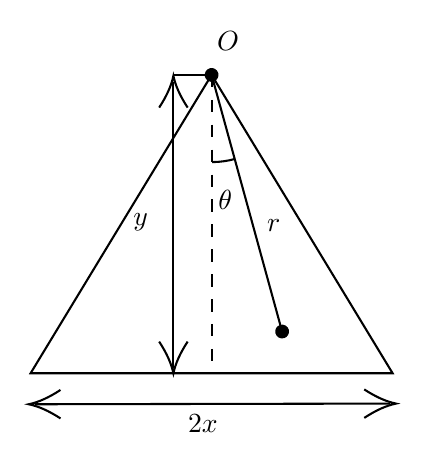
\begin{tikzpicture}[x=0.75pt,y=0.75pt,yscale=-1.4,xscale=1.4]
%uncomment if require: \path (0,159); %set diagram left start at 0, and has height of 159

%Shape: Triangle [id:dp3429465666743179] 
\draw   (350.62,21.3) -- (412.91,123.97) -- (288.33,123.97) -- cycle ;
%Straight Lines [id:da03944346674330523] 
\draw  [dash pattern={on 4.5pt off 4.5pt}]  (350.62,21.3) -- (350.62,123.64) ;
%Straight Lines [id:da7626616502789927] 
\draw    (350.62,21.3) -- (374.88,109.61) ;
\draw [shift={(374.88,109.61)}, rotate = 74.64] [color={rgb, 255:red, 0; green, 0; blue, 0 }  ][fill={rgb, 255:red, 0; green, 0; blue, 0 }  ][line width=0.75]      (0, 0) circle [x radius= 2.01, y radius= 2.01]   ;
\draw [shift={(350.62,21.3)}, rotate = 74.64] [color={rgb, 255:red, 0; green, 0; blue, 0 }  ][fill={rgb, 255:red, 0; green, 0; blue, 0 }  ][line width=0.75]      (0, 0) circle [x radius= 2.01, y radius= 2.01]   ;
%Shape: Arc [id:dp8405823847664362] 
\draw  [draw opacity=0] (358.65,50.22) .. controls (356.15,50.91) and (353.53,51.29) .. (350.82,51.3) -- (350.62,21.3) -- cycle ; \draw   (358.65,50.22) .. controls (356.15,50.91) and (353.53,51.29) .. (350.82,51.3) ;
%Straight Lines [id:da22612108938980247] 
\draw    (337.47,23.61) -- (337.47,122.01) ;
\draw [shift={(337.47,124.01)}, rotate = 270] [color={rgb, 255:red, 0; green, 0; blue, 0 }  ][line width=0.75]    (10.93,-4.9) .. controls (6.95,-2.3) and (3.31,-0.67) .. (0,0) .. controls (3.31,0.67) and (6.95,2.3) .. (10.93,4.9)   ;
\draw [shift={(337.47,21.61)}, rotate = 90] [color={rgb, 255:red, 0; green, 0; blue, 0 }  ][line width=0.75]    (10.93,-4.9) .. controls (6.95,-2.3) and (3.31,-0.67) .. (0,0) .. controls (3.31,0.67) and (6.95,2.3) .. (10.93,4.9)   ;
%Straight Lines [id:da9093229799080478] 
\draw    (337.62,21.3) -- (350.62,21.3) ;
%Straight Lines [id:da7717951632771531] 
\draw    (289.68,134.64) -- (412.08,134.41) ;
\draw [shift={(414.08,134.41)}, rotate = 539.89] [color={rgb, 255:red, 0; green, 0; blue, 0 }  ][line width=0.75]    (10.93,-4.9) .. controls (6.95,-2.3) and (3.31,-0.67) .. (0,0) .. controls (3.31,0.67) and (6.95,2.3) .. (10.93,4.9)   ;
\draw [shift={(287.68,134.64)}, rotate = 359.89] [color={rgb, 255:red, 0; green, 0; blue, 0 }  ][line width=0.75]    (10.93,-4.9) .. controls (6.95,-2.3) and (3.31,-0.67) .. (0,0) .. controls (3.31,0.67) and (6.95,2.3) .. (10.93,4.9)   ;


% Text Node
\draw (351.47,5.4) node [anchor=north west][inner sep=0.75pt]    {$O$};
% Text Node
\draw (351.87,59.91) node [anchor=north west][inner sep=0.75pt]    {$\theta $};
% Text Node
\draw (368.67,70.11) node [anchor=north west][inner sep=0.75pt]    {$r$};
% Text Node
\draw (341.47,137.04) node [anchor=north west][inner sep=0.75pt]    {$2x$};
% Text Node
\draw (322.67,67.96) node [anchor=north west][inner sep=0.75pt]    {$y$};
\end{tikzpicture}}
  
Ta có thể chia hình chữ nhật thành bốn hình tam giác cân khác bằng cách cắt hình chữ nhật dọc theo các đường chéo của hình chữ nhật.
\begin{center}

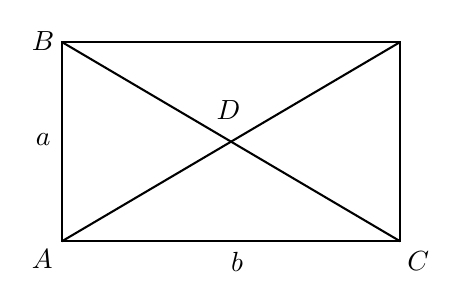
\begin{tikzpicture}[x=0.75pt,y=0.75pt,yscale=-1,xscale=1]
%uncomment if require: \path (0,144); %set diagram left start at 0, and has height of 144

%Shape: Rectangle [id:dp14314185362078402] 
\draw   (270,18.82) -- (432.97,18.82) -- (432.97,114.82) -- (270,114.82) -- cycle ;
%Straight Lines [id:da04292265530629358] 
\draw    (270,18.82) -- (432.97,114.82) ;
%Straight Lines [id:da8086631645730789] 
\draw    (270,114.82) -- (432.97,18.82) ;

% Text Node
\draw (254,117.4) node [anchor=north west][inner sep=0.75pt]    {$A$};
% Text Node
\draw (254,12.4) node [anchor=north west][inner sep=0.75pt]    {$B$};
% Text Node
\draw (434.97,118.22) node [anchor=north west][inner sep=0.75pt]    {$C$};
% Text Node
\draw (343,45.4) node [anchor=north west][inner sep=0.75pt]    {$D$};
% Text Node
\draw (256,61.53) node [anchor=north west][inner sep=0.75pt]    {$a$};
% Text Node
\draw (350,118.53) node [anchor=north west][inner sep=0.75pt]    {$b$};


\end{tikzpicture}
\end{center}
Gọi độ dài hai cạnh của hình chữ nhật là $a$ và $b$, khi đó ta có:
$$V=\dfrac{\sigma }{2\pi\varepsilon_0}\tron{a\ln\tron{\frac{\sqrt{a^2+b^2}+b}{a}}+b\ln\tron{\dfrac{\sqrt{a^2+b^2}+a}{b}}}.$$
Với $a=5s$ và $b=12s$, ta có:
$$V=\dfrac{\sigma s}{\varepsilon_0}\tron{\dfrac{5}{2\pi}\ln 5+\frac{6}{\pi}\ln\frac{3}{2}}.$$
Vậy $\displaystyle k=\frac{5}{2\pi}\ln 5+\frac{6}{\pi}\ln\frac{3}{2}\approx 2,055.$
\end{loigiai}


\begin{vd}[Điện trường của một nửa mặt cầu tích điện]
Một nửa mặt cầu bán kính $R$ được tích điện đều với mật độ điện tích mặt $\sigma$. Tính cường độ điện trường và điện thế tại tâm vỏ cầu (gợi ý: bắt đầu từ việc tính điện trường gây ra bởi một vành mỏng tích điện đều đối với một điểm nằm trên trục của nó).
\begin{center}


\tikzset{every picture/.style={line width=0.75pt}} %set default line width to 0.75pt        

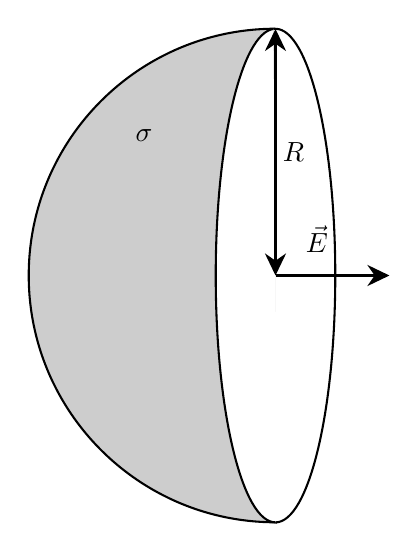
\begin{tikzpicture}[x=0.75pt,y=0.75pt,yscale=-1,xscale=1]
%uncomment if require: \path (0,480); %set diagram left start at 0, and has height of 480

%Shape: Arc [id:dp4558108973019419] 
\draw  [draw opacity=0][fill={rgb, 255:red, 155; green, 155; blue, 155 }  ,fill opacity=0.5 ] (306.71,358) .. controls (306.44,358) and (306.17,358) .. (305.9,358) .. controls (240.23,358) and (187,304.77) .. (187,239.1) .. controls (187,173.47) and (240.18,120.26) .. (305.8,120.2) -- (305.9,239.1) -- cycle ; \draw   (306.71,358) .. controls (306.44,358) and (306.17,358) .. (305.9,358) .. controls (240.23,358) and (187,304.77) .. (187,239.1) .. controls (187,173.47) and (240.18,120.26) .. (305.8,120.2) ;
%Shape: Arc [id:dp6145693508274632] 
\draw  [draw opacity=0][fill={rgb, 255:red, 255; green, 255; blue, 255 }  ,fill opacity=1 ] (306.71,358) .. controls (306.44,358.03) and (306.17,358.04) .. (305.9,358.04) .. controls (289.99,358.04) and (277.1,304.81) .. (277.1,239.14) .. controls (277.1,174.94) and (289.43,122.62) .. (304.84,120.32) -- (305.9,239.14) -- cycle ; \draw   (306.71,358) .. controls (306.44,358.03) and (306.17,358.04) .. (305.9,358.04) .. controls (289.99,358.04) and (277.1,304.81) .. (277.1,239.14) .. controls (277.1,174.94) and (289.43,122.62) .. (304.84,120.32) ;
%Shape: Arc [id:dp7833107865355216] 
\draw  [draw opacity=0][fill={rgb, 255:red, 255; green, 255; blue, 255 }  ,fill opacity=1 ] (305.09,120.29) .. controls (305.36,120.26) and (305.63,120.24) .. (305.9,120.24) .. controls (321.81,120.24) and (334.7,173.48) .. (334.7,239.14) .. controls (334.7,304.67) and (321.86,357.81) .. (306,358.04) -- (305.9,239.14) -- cycle ; \draw   (305.09,120.29) .. controls (305.36,120.26) and (305.63,120.24) .. (305.9,120.24) .. controls (321.81,120.24) and (334.7,173.48) .. (334.7,239.14) .. controls (334.7,304.67) and (321.86,357.81) .. (306,358.04) ;
%Straight Lines [id:da4909585902864282] 
\draw    (305.9,239.1) -- (357.8,239.1) ;
\draw [shift={(360.8,239.1)}, rotate = 180] [fill={rgb, 255:red, 0; green, 0; blue, 0 }  ][line width=0.08]  [draw opacity=0] (10.72,-5.15) -- (0,0) -- (10.72,5.15) -- (7.12,0) -- cycle    ;
%Straight Lines [id:da4200215184512581] 
\draw    (305.9,123.32) -- (305.9,236.1) ;
\draw [shift={(305.9,239.1)}, rotate = 270] [fill={rgb, 255:red, 0; green, 0; blue, 0 }  ][line width=0.08]  [draw opacity=0] (10.72,-5.15) -- (0,0) -- (10.72,5.15) -- (7.12,0) -- cycle    ;
\draw [shift={(305.9,120.32)}, rotate = 90] [fill={rgb, 255:red, 0; green, 0; blue, 0 }  ][line width=0.08]  [draw opacity=0] (10.72,-5.15) -- (0,0) -- (10.72,5.15) -- (7.12,0) -- cycle    ;


% Text Node
\draw (308,173.4) node [anchor=north west][inner sep=0.75pt]    {$R$};
% Text Node
\draw (319,213.4) node [anchor=north west][inner sep=0.75pt]    {$\vec{E}$};
% Text Node
\draw (237,167.4) node [anchor=north west][inner sep=0.75pt]    {$\sigma $};


\end{tikzpicture}
\end{center}

\end{vd}
\begin{loigiai}
Chúng ta bắt đầu từ điện trường gây ra bởi một vành mỏng tích điện bán kính $a$ và mật độ điện dài $\lambda$ gây ra tại một điểm $P$ nằm trên trục của nó, ở khoảng cách $x$ từ tâm $O$ của vòng dây (xem hình vẽ). Ta lấy một vi phân cung tròn dài $\dd l$, được tích điện $\lambda \dd l$, gây ra một điện trường $\dd \ot{E}$ tại điểm $P$. Độ lớn của $\dd \ot{E}$ là:
   \[ \dd E = k_e \frac{\lambda \dd l}{a^2 + x^2} . \tag{1}\]

    \begin{center}


\tikzset{every picture/.style={line width=0.75pt}} %set default line width to 0.75pt        

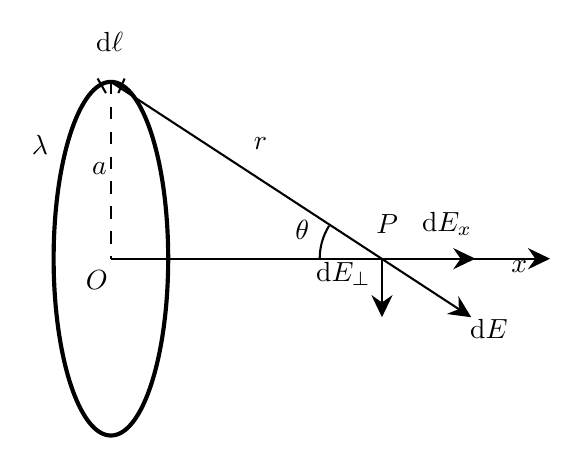
\begin{tikzpicture}[x=0.75pt,y=0.75pt,yscale=-1,xscale=1]
%uncomment if require: \path (0,480); %set diagram left start at 0, and has height of 480

%Shape: Ellipse [id:dp7943577007686424] 
\draw  [line width=1.5]  (113,191.2) .. controls (113,144.15) and (125.36,106) .. (140.6,106) .. controls (155.84,106) and (168.2,144.15) .. (168.2,191.2) .. controls (168.2,238.25) and (155.84,276.4) .. (140.6,276.4) .. controls (125.36,276.4) and (113,238.25) .. (113,191.2) -- cycle ;
%Straight Lines [id:da050784527645520994] 
\draw    (140.6,191.2) -- (349.2,191.2) ;
\draw [shift={(352.2,191.2)}, rotate = 180] [fill={rgb, 255:red, 0; green, 0; blue, 0 }  ][line width=0.08]  [draw opacity=0] (10.72,-5.15) -- (0,0) -- (10.72,5.15) -- (7.12,0) -- cycle    ;
%Straight Lines [id:da996198800097212] 
\draw  [dash pattern={on 4.5pt off 4.5pt}]  (140.6,106) -- (140.6,191.2) ;
%Straight Lines [id:da7771722324877135] 
\draw    (134.2,104.4) -- (138.2,111.4) ;
%Straight Lines [id:da4133881703636635] 
\draw    (147.2,104.4) -- (144.2,111.4) ;
%Straight Lines [id:da2435636005783719] 
\draw    (140.6,106) -- (311.69,217.76) ;
\draw [shift={(314.2,219.4)}, rotate = 213.15] [fill={rgb, 255:red, 0; green, 0; blue, 0 }  ][line width=0.08]  [draw opacity=0] (10.72,-5.15) -- (0,0) -- (10.72,5.15) -- (7.12,0) -- cycle    ;
%Straight Lines [id:da6896149995797138] 
\draw    (271.2,191.2) -- (271.2,216.4) ;
\draw [shift={(271.2,219.4)}, rotate = 270] [fill={rgb, 255:red, 0; green, 0; blue, 0 }  ][line width=0.08]  [draw opacity=0] (10.72,-5.15) -- (0,0) -- (10.72,5.15) -- (7.12,0) -- cycle    ;
%Straight Lines [id:da0004949043224988792] 
\draw    (271.2,191.2) -- (313.2,191.2) ;
\draw [shift={(316.2,191.2)}, rotate = 180] [fill={rgb, 255:red, 0; green, 0; blue, 0 }  ][line width=0.08]  [draw opacity=0] (10.72,-5.15) -- (0,0) -- (10.72,5.15) -- (7.12,0) -- cycle    ;
%Shape: Arc [id:dp2981728301376838] 
\draw  [draw opacity=0] (241.2,191.37) .. controls (241.2,191.31) and (241.2,191.26) .. (241.2,191.2) .. controls (241.2,185.38) and (242.86,179.95) .. (245.72,175.35) -- (271.2,191.2) -- cycle ; \draw   (241.2,191.37) .. controls (241.2,191.31) and (241.2,191.26) .. (241.2,191.2) .. controls (241.2,185.38) and (242.86,179.95) .. (245.72,175.35) ;



% Text Node
\draw (101,130.4) node [anchor=north west][inner sep=0.75pt]    {$\lambda $};
% Text Node
\draw (127,195.4) node [anchor=north west][inner sep=0.75pt]    {$O$};
% Text Node
\draw (130,143.4) node [anchor=north west][inner sep=0.75pt]    {$a$};
% Text Node
\draw (132,80.4) node [anchor=north west][inner sep=0.75pt]    {$\mathrm{d} \ell $};
% Text Node
\draw (208,131.4) node [anchor=north west][inner sep=0.75pt]    {$r$};
% Text Node
\draw (267,168.4) node [anchor=north west][inner sep=0.75pt]    {$P$};
% Text Node
\draw (289,167.4) node [anchor=north west][inner sep=0.75pt]    {$\mathrm{d} E_{x}$};
% Text Node
\draw (238,191.4) node [anchor=north west][inner sep=0.75pt]    {$\mathrm{d} E_{\bot }$};
% Text Node
\draw (312.2,218.8) node [anchor=north west][inner sep=0.75pt]    {$\mathrm{d}\ot{E}$};
% Text Node
\draw (228,171.4) node [anchor=north west][inner sep=0.75pt]    {$\theta $};
% Text Node
\draw (332,190.4) node [anchor=north west][inner sep=0.75pt]    {$x$};


\end{tikzpicture}
\end{center}
Vi phân điện trường  $\dd \ot{E}$ có thành phần $\dd E_x$ song song với trục của vành và thành phần $\dd E_{\perp}$  vuông góc với trục. Chúng ta chỉ cần tính đến thành phần song song của điện trường:
\[\begin{aligned}
 \dd E_x & = \cos \theta \dd E = k_e \frac{\lambda \dd l}{a^2 + x^2} \frac{x}{\sqrt{a^2 + x^2}} \\
    &= k_e \frac{\lambda x \dd l}{(a^2 + x^2)^{3/2}} , \end{aligned} \tag{2}\]

bởi vì thành phần vuông góc sẽ tự triệt tiêu lẫn nhau khi chúng ta tích phân quanh vành mảnh. Khi tích phân, các biến $\theta$ và $r$ không phụ thuộc vào vị trí của $\dd l$, do đó điện trường tổng cộng tại $P$ là:
  \[\begin{aligned} E_x &= k_e \frac{\lambda x}{(a^2 + x^2)^{3/2}} \int_{0}^{2\pi a} \dd l = k_e  \frac{2\pi a \lambda x}{(a^2 +x^2)^{3/2}} \\
  \\
                &= \left\{ \begin{array}{cc} \dfrac{1}{4\pi \varepsilon_0} \dfrac{2\pi a \lambda x}{(a^2+x^2)^{3/2}}   & \text{SI} \\
                \\
                 \dfrac{2\pi a \lambda x}{(a^2+x^2)^{3/2}}  & \text{Gaussian}, \end{array} \right.  \end{aligned} \tag{3} \]

Biểu thức có thể được viết lại thành: 
     \[  \ot{E} = \hat{{x}} k_e \frac{Qx}{(a^2 + x^2)^{3/2}}, \tag{4} \]
ở đây $Q=2\pi a \lambda$ là tổng điện tích của vành.
   \begin{center}


\tikzset{every picture/.style={line width=0.75pt}} %set default line width to 0.75pt        

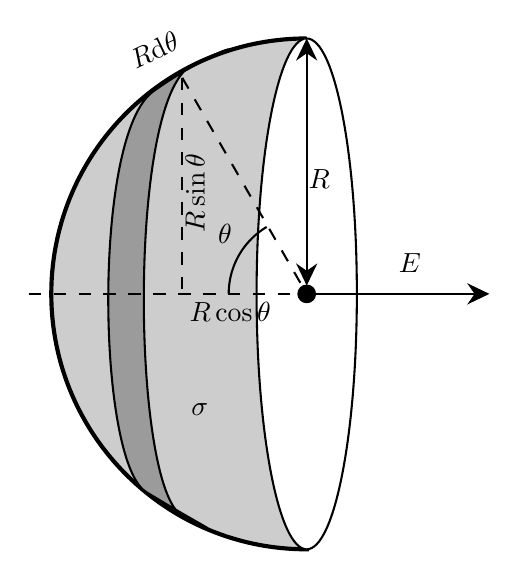
\begin{tikzpicture}[x=0.75pt,y=0.75pt,yscale=-1,xscale=1]
%uncomment if require: \path (0,480); %set diagram left start at 0, and has height of 480

%Shape: Arc [id:dp9751651413882021] 
\draw  [draw opacity=0][fill={rgb, 255:red, 155; green, 155; blue, 155 }  ,fill opacity=0.5 ][line width=1.5]  (240.95,352.76) .. controls (240.61,352.76) and (240.28,352.76) .. (239.94,352.76) .. controls (171.98,352.76) and (116.88,297.67) .. (116.88,229.7) .. controls (116.88,161.74) and (171.98,106.64) .. (239.94,106.64) -- (239.94,229.7) -- cycle ; \draw  [line width=1.5]  (240.95,352.76) .. controls (240.61,352.76) and (240.28,352.76) .. (239.94,352.76) .. controls (171.98,352.76) and (116.88,297.67) .. (116.88,229.7) .. controls (116.88,161.74) and (171.98,106.64) .. (239.94,106.64) ;
%Shape: Arc [id:dp07613452841355706] 
\draw  [draw opacity=0][fill={rgb, 255:red, 255; green, 255; blue, 255 }  ,fill opacity=1 ] (240.95,352.66) .. controls (240.61,352.73) and (240.28,352.76) .. (239.94,352.76) .. controls (226.6,352.76) and (215.79,297.67) .. (215.79,229.7) .. controls (215.79,161.74) and (226.6,106.64) .. (239.94,106.64) -- (239.94,229.7) -- cycle ; \draw   (240.95,352.66) .. controls (240.61,352.73) and (240.28,352.76) .. (239.94,352.76) .. controls (226.6,352.76) and (215.79,297.67) .. (215.79,229.7) .. controls (215.79,161.74) and (226.6,106.64) .. (239.94,106.64) ;
%Shape: Arc [id:dp11615013675617436] 
\draw  [draw opacity=0][fill={rgb, 255:red, 255; green, 255; blue, 255 }  ,fill opacity=1 ] (238.93,106.75) .. controls (239.27,106.68) and (239.6,106.64) .. (239.94,106.64) .. controls (253.28,106.64) and (264.1,161.74) .. (264.1,229.7) .. controls (264.1,297.67) and (253.28,352.76) .. (239.94,352.76) -- (239.94,229.7) -- cycle ; \draw   (238.93,106.75) .. controls (239.27,106.68) and (239.6,106.64) .. (239.94,106.64) .. controls (253.28,106.64) and (264.1,161.74) .. (264.1,229.7) .. controls (264.1,297.67) and (253.28,352.76) .. (239.94,352.76) ;
%Shape: Polygon Curved [id:ds027284506820421495] 
\draw  [fill={rgb, 255:red, 155; green, 155; blue, 155 }  ,fill opacity=1 ] (166.06,132.1) .. controls (195.66,111) and (218.07,106.43) .. (185.65,119.05) .. controls (153.22,131.67) and (155.4,324.26) .. (180.21,336.66) .. controls (205.01,349.06) and (186.3,339.71) .. (162.58,325.13) .. controls (138.86,310.55) and (136.47,153.21) .. (166.06,132.1) -- cycle ;
%Straight Lines [id:da13270213954243215] 
\draw  [dash pattern={on 4.5pt off 4.5pt}]  (106,229.7) -- (239.94,229.7) ;
%Straight Lines [id:da6043344427332653] 
\draw    (239.94,229.7) -- (324.96,229.7) ;
\draw [shift={(327.96,229.7)}, rotate = 180] [fill={rgb, 255:red, 0; green, 0; blue, 0 }  ][line width=0.08]  [draw opacity=0] (10.72,-5.15) -- (0,0) -- (10.72,5.15) -- (7.12,0) -- cycle    ;
%Straight Lines [id:da9380275362339183] 
\draw    (239.94,109.64) -- (239.94,222.7) ;
\draw [shift={(239.94,225.7)}, rotate = 270] [fill={rgb, 255:red, 0; green, 0; blue, 0 }  ][line width=0.08]  [draw opacity=0] (10.72,-5.15) -- (0,0) -- (10.72,5.15) -- (7.12,0) -- cycle    ;
\draw [shift={(239.94,106.64)}, rotate = 90] [fill={rgb, 255:red, 0; green, 0; blue, 0 }  ][line width=0.08]  [draw opacity=0] (10.72,-5.15) -- (0,0) -- (10.72,5.15) -- (7.12,0) -- cycle    ;
%Straight Lines [id:da058284329477305] 
\draw  [dash pattern={on 4.5pt off 4.5pt}]  (179.99,125.58) -- (239.94,229.7) ;
%Straight Lines [id:da9260211082999852] 
\draw  [dash pattern={on 4.5pt off 4.5pt}]  (179.99,125.58) -- (179.99,228.94) ;
%Shape: Arc [id:dp5834096030996945] 
\draw  [draw opacity=0] (202.35,229.53) .. controls (202.35,228.36) and (202.41,227.17) .. (202.53,225.98) .. controls (203.76,213.67) and (210.79,203.34) .. (220.64,197.44) -- (239.94,229.7) -- cycle ; \draw   (202.35,229.53) .. controls (202.35,228.36) and (202.41,227.17) .. (202.53,225.98) .. controls (203.76,213.67) and (210.79,203.34) .. (220.64,197.44) ;
%Shape: Circle [id:dp5905363482755994] 
\draw  [fill={rgb, 255:red, 0; green, 0; blue, 0 }  ,fill opacity=1 ] (235.94,229.7) .. controls (235.94,227.49) and (237.73,225.7) .. (239.94,225.7) .. controls (242.15,225.7) and (243.94,227.49) .. (243.94,229.7) .. controls (243.94,231.91) and (242.15,233.7) .. (239.94,233.7) .. controls (237.73,233.7) and (235.94,231.91) .. (235.94,229.7) -- cycle ;


% Text Node
\draw (151.58,112.64) node [anchor=north west][inner sep=0.75pt]  [rotate=-334.21]  {$R\mathrm{d} \theta $};
% Text Node
\draw (239.33,168.38) node [anchor=north west][inner sep=0.75pt]    {$R$};
% Text Node
\draw (282.84,208.94) node [anchor=north west][inner sep=0.75pt]    {$\ot{E}$};
% Text Node
\draw (180.04,201.43) node [anchor=north west][inner sep=0.75pt]  [rotate=-270]  {$R\sin \theta $};
% Text Node
\draw (195.7,194.67) node [anchor=north west][inner sep=0.75pt]    {$\theta $};
% Text Node
\draw (182.92,281.28) node [anchor=north west][inner sep=0.75pt]    {$\ot{\sigma }$};
% Text Node
\draw (181.99,232.34) node [anchor=north west][inner sep=0.75pt]    {$R\cos \theta $};


\end{tikzpicture}
\end{center}
Mặt cầu tích điện có thể được chia thành các vành mảnh vi phân giữa các góc phương vị $\theta$ và $\theta + \dd \theta$ vì tính đối xứng của bán cầu (xem hình vẽ). Mỗi vành mỏng tương tự như một vòng tích điện có bán kính $R\sin \theta$ và điện tích tổng cộng $\dd Q = \sigma 2 \pi R^2 \sin \theta \dd \theta $. Tâm của bán cầu nằm trên trục đối xứng của vành mỏng, ở khoảng cách $x= R \cos \theta$ từ tâm của mỗi vành. Do đó, đóng góp của mỗi vành mỏng cho điện trường ở tâm bán cầu là: 
    \[\begin{aligned} \dd E & = k_e \dfrac{\sigma 2 \pi R^2 \sin \theta \dd \theta R \cos \theta}{(R^2 \sin^2 \theta + R^2 \cos^2\theta)^{3/2}} \\
        & =  k_e \dfrac{\sigma 2 \pi R^3 \cos \theta \sin \theta \dd \theta}{R^3} = k_e \sigma 2 \pi \cos \theta \sin \theta \dd \theta, \end{aligned} \tag{5} \]

và điện trường tổng cộng là:
       \[ E = k_e  \sigma  2 \pi \int_{0}^{\pi/2} \cos \theta \sin \theta \dd \theta = k_e \pi \sigma, \tag{6} \]

không phụ thuộc vào bán kính $R$. Ta cũng làm tương tự với điện thế tại tâm bán cầu.
\end{loigiai}

\begin{vd}[Điện trường của vỏ cầu tích điện]
    \label{ca5}
    Xét điện trường tạo ra bởi một vỏ cầu rỗng tích điện đều với điện tích $Q$. Chúng ta có thể tìm được điện trường do vỏ cầu gây ra tại một điểm bên trong hoặc bên ngoài vỏ cầu bằng cách sử dụng định luật Gauss. Trong bài này, chúng ta sẽ đi tìm điện trường bằng một cách khác. Hãy tính điện thế $\phi(r)$ của một điểm cách tâm vỏ cầu một khoảng $r$ bằng cách chia vỏ cầu thành các phần tử diện tích nhỏ rồi tích phân điện thế do từng phần tử đóng góp vào điện thế tại điểm đang tính. Điện trường tại điểm đó có thể tìm được bằng công thức $E(r)=-\dfrac{\dd \phi}{\dd r}$.\\ 
    \begin{center}
        

\tikzset{every picture/.style={line width=0.75pt}} %set default line width to 0.75pt        

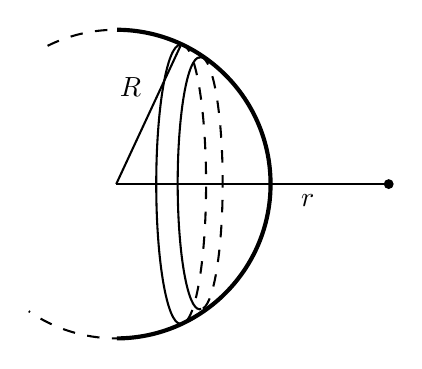
\begin{tikzpicture}[x=0.75pt,y=0.75pt,yscale=-1,xscale=1]
%uncomment if require: \path (0,221); %set diagram left start at 0, and has height of 221

%Shape: Arc [id:dp9180859117676652] 
\draw  [draw opacity=0][line width=1.5]  (287.74,27) .. controls (328.63,27.21) and (361.71,60.42) .. (361.71,101.35) .. controls (361.71,142.31) and (328.6,175.53) .. (287.69,175.71) -- (287.35,101.35) -- cycle ; \draw  [line width=1.5]  (287.74,27) .. controls (328.63,27.21) and (361.71,60.42) .. (361.71,101.35) .. controls (361.71,142.31) and (328.6,175.53) .. (287.69,175.71) ;
%Shape: Arc [id:dp9949488668982875] 
\draw  [draw opacity=0][dash pattern={on 4.5pt off 4.5pt}][line width=0.75]  (254.27,34.75) .. controls (264.24,29.79) and (275.47,27) .. (287.35,27) .. controls (328.42,27) and (361.71,60.29) .. (361.71,101.35) .. controls (361.71,142.42) and (328.42,175.71) .. (287.35,175.71) .. controls (271.7,175.71) and (257.17,170.87) .. (245.19,162.61) -- (287.35,101.35) -- cycle ; \draw  [dash pattern={on 4.5pt off 4.5pt}][line width=0.75]  (254.27,34.75) .. controls (264.24,29.79) and (275.47,27) .. (287.35,27) .. controls (328.42,27) and (361.71,60.29) .. (361.71,101.35) .. controls (361.71,142.42) and (328.42,175.71) .. (287.35,175.71) .. controls (271.7,175.71) and (257.17,170.87) .. (245.19,162.61) ;
%Shape: Arc [id:dp6320579717276376] 
\draw  [draw opacity=0] (328.3,161.49) .. controls (328.04,161.61) and (327.77,161.67) .. (327.5,161.67) .. controls (321.68,161.67) and (316.96,134.5) .. (316.96,100.99) .. controls (316.96,67.47) and (321.68,40.31) .. (327.5,40.31) .. controls (327.58,40.31) and (327.66,40.31) .. (327.73,40.32) -- (327.5,100.99) -- cycle ; \draw   (328.3,161.49) .. controls (328.04,161.61) and (327.77,161.67) .. (327.5,161.67) .. controls (321.68,161.67) and (316.96,134.5) .. (316.96,100.99) .. controls (316.96,67.47) and (321.68,40.31) .. (327.5,40.31) .. controls (327.58,40.31) and (327.66,40.31) .. (327.73,40.32) ;
%Shape: Arc [id:dp7997514267193591] 
\draw  [draw opacity=0][dash pattern={on 4.5pt off 4.5pt}] (327.3,40.43) .. controls (327.56,40.31) and (327.83,40.25) .. (328.1,40.25) .. controls (333.92,40.25) and (338.64,67.42) .. (338.64,100.93) .. controls (338.64,134.45) and (333.92,161.61) .. (328.1,161.61) .. controls (328.02,161.61) and (327.94,161.61) .. (327.86,161.6) -- (328.1,100.93) -- cycle ; \draw  [dash pattern={on 4.5pt off 4.5pt}] (327.3,40.43) .. controls (327.56,40.31) and (327.83,40.25) .. (328.1,40.25) .. controls (333.92,40.25) and (338.64,67.42) .. (338.64,100.93) .. controls (338.64,134.45) and (333.92,161.61) .. (328.1,161.61) .. controls (328.02,161.61) and (327.94,161.61) .. (327.86,161.6) ;

%Shape: Arc [id:dp06962011240073829] 
\draw  [draw opacity=0] (319.19,168.47) .. controls (318.9,168.6) and (318.6,168.67) .. (318.3,168.67) .. controls (311.86,168.67) and (306.63,138.57) .. (306.63,101.45) .. controls (306.63,64.33) and (311.86,34.24) .. (318.3,34.24) .. controls (318.39,34.24) and (318.47,34.25) .. (318.56,34.26) -- (318.3,101.45) -- cycle ; \draw   (319.19,168.47) .. controls (318.9,168.6) and (318.6,168.67) .. (318.3,168.67) .. controls (311.86,168.67) and (306.63,138.57) .. (306.63,101.45) .. controls (306.63,64.33) and (311.86,34.24) .. (318.3,34.24) .. controls (318.39,34.24) and (318.47,34.25) .. (318.56,34.26) ;
%Shape: Arc [id:dp44336333675449535] 
\draw  [draw opacity=0][dash pattern={on 4.5pt off 4.5pt}] (318.07,34.38) .. controls (318.37,34.25) and (318.66,34.18) .. (318.96,34.18) .. controls (325.41,34.18) and (330.64,64.28) .. (330.64,101.4) .. controls (330.64,138.52) and (325.41,168.61) .. (318.96,168.61) .. controls (318.88,168.61) and (318.79,168.6) .. (318.71,168.59) -- (318.96,101.4) -- cycle ; \draw  [dash pattern={on 4.5pt off 4.5pt}] (318.07,34.38) .. controls (318.37,34.25) and (318.66,34.18) .. (318.96,34.18) .. controls (325.41,34.18) and (330.64,64.28) .. (330.64,101.4) .. controls (330.64,138.52) and (325.41,168.61) .. (318.96,168.61) .. controls (318.88,168.61) and (318.79,168.6) .. (318.71,168.59) ;

%Straight Lines [id:da839400938864665] 
\draw    (287.35,101.35) -- (418.64,101.35) ;
%Straight Lines [id:da06623462412375702] 
\draw    (318.56,34.26) -- (287.35,101.35) ;
%Shape: Circle [id:dp567051033556494] 
\draw  [fill={rgb, 255:red, 0; green, 0; blue, 0 }  ,fill opacity=1 ] (416.8,101.35) .. controls (416.8,100.34) and (417.62,99.52) .. (418.64,99.52) .. controls (419.65,99.52) and (420.47,100.34) .. (420.47,101.35) .. controls (420.47,102.37) and (419.65,103.19) .. (418.64,103.19) .. controls (417.62,103.19) and (416.8,102.37) .. (416.8,101.35) -- cycle ;

% Text Node
\draw (374.96,105) node [anchor=north west][inner sep=0.75pt]    {$r$};
% Text Node
\draw (287.63,48.4) node [anchor=north west][inner sep=0.75pt]    {$R$};


\end{tikzpicture}

    \end{center}
    \textit{Gợi ý: Cách đơn giản nhất đó chính là chia vỏ cầu thành nhiều vòng nhỏ như trên hình.}
    \end{vd}
    \begin{loigiai}\\
    \begin{center}
        

\tikzset{every picture/.style={line width=0.75pt}} %set default line width to 0.75pt        

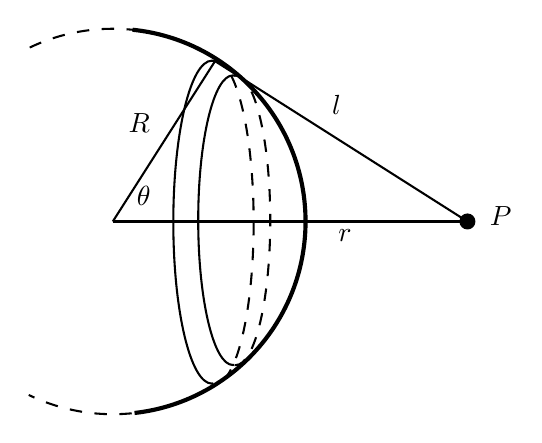
\begin{tikzpicture}[x=0.75pt,y=0.75pt,yscale=-1,xscale=1]
%uncomment if require: \path (0,300); %set diagram left start at 0, and has height of 300

%Shape: Arc [id:dp6604130734699976] 
\draw  [draw opacity=0][line width=1.5]  (338.38,47.48) .. controls (385.19,52.25) and (421.71,91.79) .. (421.71,139.85) .. controls (421.71,187.6) and (385.67,226.93) .. (339.32,232.12) -- (328.85,139.85) -- cycle ; \draw  [line width=1.5]  (338.38,47.48) .. controls (385.19,52.25) and (421.71,91.79) .. (421.71,139.85) .. controls (421.71,187.6) and (385.67,226.93) .. (339.32,232.12) ;
%Shape: Arc [id:dp3988355543248949] 
\draw  [draw opacity=0][dash pattern={on 4.5pt off 4.5pt}] (288.83,56.05) .. controls (300.95,50.25) and (314.52,47) .. (328.85,47) .. controls (380.14,47) and (421.71,88.57) .. (421.71,139.85) .. controls (421.71,191.14) and (380.14,232.71) .. (328.85,232.71) .. controls (314.33,232.71) and (300.59,229.37) .. (288.34,223.43) -- (328.85,139.85) -- cycle ; \draw  [dash pattern={on 4.5pt off 4.5pt}] (288.83,56.05) .. controls (300.95,50.25) and (314.52,47) .. (328.85,47) .. controls (380.14,47) and (421.71,88.57) .. (421.71,139.85) .. controls (421.71,191.14) and (380.14,232.71) .. (328.85,232.71) .. controls (314.33,232.71) and (300.59,229.37) .. (288.34,223.43) ;
%Shape: Arc [id:dp3770531364912999] 
\draw  [draw opacity=0] (377.32,217.94) .. controls (377.09,217.98) and (376.86,217.99) .. (376.63,217.99) .. controls (366.34,217.99) and (358,183.16) .. (358,140.18) .. controls (358,97.21) and (366.34,62.37) .. (376.63,62.37) .. controls (377.13,62.37) and (377.62,62.45) .. (378.11,62.61) -- (376.63,140.18) -- cycle ; \draw   (377.32,217.94) .. controls (377.09,217.98) and (376.86,217.99) .. (376.63,217.99) .. controls (366.34,217.99) and (358,183.16) .. (358,140.18) .. controls (358,97.21) and (366.34,62.37) .. (376.63,62.37) .. controls (377.13,62.37) and (377.62,62.45) .. (378.11,62.61) ;
%Shape: Arc [id:dp48119814484050627] 
\draw  [draw opacity=0][dash pattern={on 4.5pt off 4.5pt}] (377.38,62.51) .. controls (377.61,62.47) and (377.84,62.46) .. (378.08,62.46) .. controls (388.37,62.46) and (396.71,97.29) .. (396.71,140.27) .. controls (396.71,183.24) and (388.37,218.08) .. (378.08,218.08) .. controls (377.58,218.08) and (377.09,218) .. (376.6,217.84) -- (378.08,140.27) -- cycle ; \draw  [dash pattern={on 4.5pt off 4.5pt}] (377.38,62.51) .. controls (377.61,62.47) and (377.84,62.46) .. (378.08,62.46) .. controls (388.37,62.46) and (396.71,97.29) .. (396.71,140.27) .. controls (396.71,183.24) and (388.37,218.08) .. (378.08,218.08) .. controls (377.58,218.08) and (377.09,218) .. (376.6,217.84) ;

%Shape: Arc [id:dp38971002723714365] 
\draw  [draw opacity=0] (387.33,208.95) .. controls (387.12,208.99) and (386.91,209) .. (386.71,209) .. controls (377.48,209) and (370,177.77) .. (370,139.23) .. controls (370,100.7) and (377.48,69.46) .. (386.71,69.46) .. controls (387.15,69.46) and (387.59,69.54) .. (388.03,69.68) -- (386.71,139.23) -- cycle ; \draw   (387.33,208.95) .. controls (387.12,208.99) and (386.91,209) .. (386.71,209) .. controls (377.48,209) and (370,177.77) .. (370,139.23) .. controls (370,100.7) and (377.48,69.46) .. (386.71,69.46) .. controls (387.15,69.46) and (387.59,69.54) .. (388.03,69.68) ;
%Shape: Arc [id:dp7448302847473949] 
\draw  [draw opacity=0][dash pattern={on 4.5pt off 4.5pt}] (387.38,69.59) .. controls (387.59,69.55) and (387.79,69.54) .. (388,69.54) .. controls (397.23,69.54) and (404.71,100.78) .. (404.71,139.31) .. controls (404.71,177.84) and (397.23,209.08) .. (388,209.08) .. controls (387.56,209.08) and (387.11,209) .. (386.68,208.86) -- (388,139.31) -- cycle ; \draw  [dash pattern={on 4.5pt off 4.5pt}] (387.38,69.59) .. controls (387.59,69.55) and (387.79,69.54) .. (388,69.54) .. controls (397.23,69.54) and (404.71,100.78) .. (404.71,139.31) .. controls (404.71,177.84) and (397.23,209.08) .. (388,209.08) .. controls (387.56,209.08) and (387.11,209) .. (386.68,208.86) ;

%Straight Lines [id:da6172667981511248] 
\draw    (328.85,139.85) -- (499.71,139.85) ;
\draw [shift={(499.71,139.85)}, rotate = 0] [color={rgb, 255:red, 0; green, 0; blue, 0 }  ][fill={rgb, 255:red, 0; green, 0; blue, 0 }  ][line width=0.75]      (0, 0) circle [x radius= 3.35, y radius= 3.35]   ;
%Straight Lines [id:da567536953964995] 
\draw    (378.11,62.61) -- (328.85,139.85) ;
%Straight Lines [id:da6026285341166078] 
\draw    (378.11,62.61) -- (499.71,139.85) ;

% Text Node
\draw (339,121.4) node [anchor=north west][inner sep=0.75pt]    {$\theta $};
% Text Node
\draw (335,86.4) node [anchor=north west][inner sep=0.75pt]    {$R$};
% Text Node
\draw (436,142.4) node [anchor=north west][inner sep=0.75pt]    {$r$};
% Text Node
\draw (433,77.4) node [anchor=north west][inner sep=0.75pt]    {$l$};
% Text Node
\draw (509,131.4) node [anchor=north west][inner sep=0.75pt]    {$P$};


\end{tikzpicture}

    \end{center}
        Xét một điểm $P$ cách tâm quả cầu một khoảng $r$ và một vòng nhỏ xác định bởi góc $\theta$ như trên hình. Khoảng cách từ điểm $P$ tới một điểm trên vòng sẽ là $l=\sqrt{R^2+r^2-2Rr\cos\theta}$. Diện tích của vòng nhỏ sẽ là $2\pi R^2 \sin\theta\dd\theta$, điện tích của vòng sẽ là $\dd Q=\sigma2\pi R^2 \sin\theta\dd\theta=\dfrac{Q\sin\theta\dd\theta}{2}$. Điện thế do vòng dây gây ra tại $P$:
        \begin{equation}
            \dd \phi=\dfrac{\dd Q}{4\pi\varepsilon_0 l}=\dfrac{Q\sin\theta\dd\theta}{8\pi\varepsilon_0\sqrt{R^2+r^2-2Rr\cos\theta}}.
        \end{equation}
        Điện thế do cả quả cầu gây ra tại $P$ sẽ là:
        \begin{equation}
            \begin{aligned}
               \phi(r)&=\dfrac{Q}{8\pi\varepsilon_0}\tiph{0}{\pi}{\dfrac{\sin\theta}{\sqrt{R^2+r^2-2Rr\cos\theta}}}{\theta}\\
               &=\left.\dfrac{Q}{8\pi\varepsilon_0Rr}\sqrt{R^2+r^2-2Rr\cos\theta}\right|_0^\pi.
            \end{aligned}
        \end{equation}
        Bây giờ chúng ta phải xét đến hai trường hợp. Nếu $r<R$ ($P$ nằm bên trong vỏ cầu), ta có:
        \begin{equation}
            \phi(r)=\dfrac{Q}{8\pi\varepsilon_0rR}\tron{(R+r)-(R-r)}=\dfrac{Q}{4\pi\varepsilon_0R}.
        \end{equation}
        Nếu $r>R$ ($P$ nằm bên ngoài vỏ cầu), ta có:
        \begin{equation}
            \phi(r)=\dfrac{Q}{8\pi\varepsilon_0rR}\tron{(R+r)-(r-R)}=\dfrac{Q}{4\pi\varepsilon_0r}.
        \end{equation}
        Ta thấy nếu $P$ nằm bên trong vỏ cầu, điện thế là một hằng số, vậy nên điện trường bên trong vỏ cầu bằng không. Khi $P$ ở bên ngoài vỏ cầu, ta có:
        \begin{equation}
            E(r)=-\dfrac{\dd \phi}{\dd r}=\dfrac{Q}{4\pi\varepsilon_0 r^2}.
        \end{equation}
        Bởi vì một quả cầu đặc tích điện trên thể tích có thể coi như là nhiều vỏ cầu nhỏ ghép lại với nhau, từ kết quả trên có thể suy ra được điện trường bên ngoài một quả cầu đặc tích điện sẽ là $\dfrac{Q}{4\pi\varepsilon_0 r^2}$, điện trường bên trong quả cầu sẽ là $\dfrac{Q_r}{4\pi\varepsilon_0 r^2}$, với $Q_r$ là phần điện tích nằm bên trong mặt cầu bán kính $r$. Điều này đúng kể cả khi phân bố điện tích là không đều.
    \end{loigiai}
    
    
     \begin{vd}[Lực điện của tam giác]
    Hai ion dương mang điện tích $+q$ và một ion âm mang điện tích $-q$ được đặt tại ba đỉnh của một tam giác đều. Tìm vị trí đặt ion thứ tư trên trục đối xứng của hệ để cho lực tác dụng lên ion này bằng không. Liệu có nhiều hơn một vị trí không?
    \end{vd}
     \begin{loigiai}
    \hfill \\
    \begin{center}
        \tikzset{every picture/.style={line width=0.75pt}} %set default line width to 0.75pt        

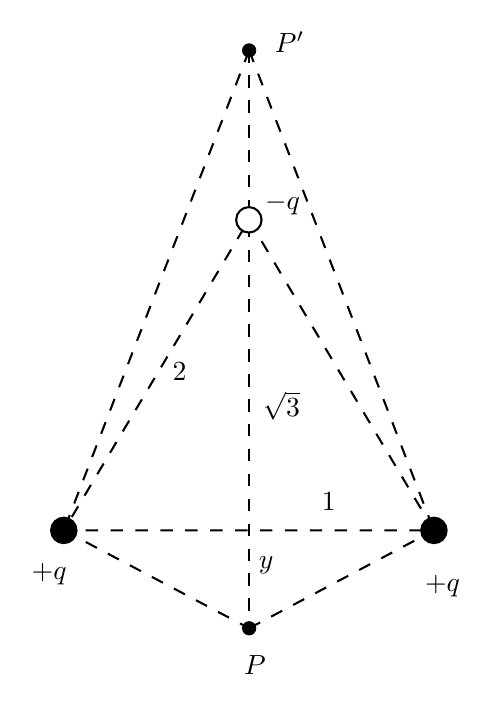
\begin{tikzpicture}[x=0.75pt,y=0.75pt,yscale=-1,xscale=1]
%uncomment if require: \path (0,379); %set diagram left start at 0, and has height of 379

%Shape: Triangle [id:dp4080380612369703] 
\draw  [dash pattern={on 4.5pt off 4.5pt}] (365.55,110.27) -- (454.71,259.9) -- (276.39,259.9) -- cycle ;
%Shape: Ellipse [id:dp8694105692535528] 
\draw  [fill={rgb, 255:red, 0; green, 0; blue, 0 }  ,fill opacity=1 ] (270.26,259.9) .. controls (270.26,256.52) and (273,253.77) .. (276.39,253.77) .. controls (279.77,253.77) and (282.51,256.52) .. (282.51,259.9) .. controls (282.51,263.28) and (279.77,266.03) .. (276.39,266.03) .. controls (273,266.03) and (270.26,263.28) .. (270.26,259.9) -- cycle ;
%Shape: Ellipse [id:dp30617169657291887] 
\draw  [fill={rgb, 255:red, 0; green, 0; blue, 0 }  ,fill opacity=1 ] (448.58,259.9) .. controls (448.58,256.52) and (451.32,253.77) .. (454.71,253.77) .. controls (458.09,253.77) and (460.83,256.52) .. (460.83,259.9) .. controls (460.83,263.28) and (458.09,266.03) .. (454.71,266.03) .. controls (451.32,266.03) and (448.58,263.28) .. (448.58,259.9) -- cycle ;
%Straight Lines [id:da8469405557870995] 
\draw  [dash pattern={on 4.5pt off 4.5pt}]  (365.68,28.64) -- (365.68,110.92) -- (365.68,309.97) ;
%Shape: Ellipse [id:dp9844313946695709] 
\draw  [fill={rgb, 255:red, 0; green, 0; blue, 0 }  ,fill opacity=1 ] (362.76,307.05) .. controls (362.76,305.44) and (364.07,304.14) .. (365.68,304.14) .. controls (367.29,304.14) and (368.6,305.44) .. (368.6,307.05) .. controls (368.6,308.67) and (367.29,309.97) .. (365.68,309.97) .. controls (364.07,309.97) and (362.76,308.67) .. (362.76,307.05) -- cycle ;
%Straight Lines [id:da4754067738293375] 
\draw  [dash pattern={on 4.5pt off 4.5pt}]  (276.39,259.9) -- (365.68,307.05) ;
%Straight Lines [id:da46350026105678754] 
\draw  [dash pattern={on 4.5pt off 4.5pt}]  (365.68,307.05) -- (454.71,259.9) ;
%Shape: Ellipse [id:dp453164314673151] 
\draw  [fill={rgb, 255:red, 0; green, 0; blue, 0 }  ,fill opacity=1 ] (362.76,28.64) .. controls (362.76,27.03) and (364.07,25.73) .. (365.68,25.73) .. controls (367.29,25.73) and (368.6,27.03) .. (368.6,28.64) .. controls (368.6,30.26) and (367.29,31.56) .. (365.68,31.56) .. controls (364.07,31.56) and (362.76,30.26) .. (362.76,28.64) -- cycle ;
%Straight Lines [id:da8751592952605081] 
\draw  [dash pattern={on 4.5pt off 4.5pt}]  (365.68,28.64) -- (276.39,259.9) ;
%Straight Lines [id:da33615571314849624] 
\draw  [dash pattern={on 4.5pt off 4.5pt}]  (365.68,28.64) -- (454.71,259.9) ;
%Shape: Ellipse [id:dp16509540062153882] 
\draw  [fill={rgb, 255:red, 255; green, 255; blue, 255 }  ,fill opacity=1 ] (359.42,110.27) .. controls (359.42,106.89) and (362.16,104.14) .. (365.55,104.14) .. controls (368.93,104.14) and (371.67,106.89) .. (371.67,110.27) .. controls (371.67,113.65) and (368.93,116.4) .. (365.55,116.4) .. controls (362.16,116.4) and (359.42,113.65) .. (359.42,110.27) -- cycle ;

% Text Node
\draw (259.48,274.4) node [anchor=north west][inner sep=0.75pt]    {$+q$};
% Text Node
\draw (448.94,280) node [anchor=north west][inner sep=0.75pt]    {$+q$};
% Text Node
\draw (368.9,271.2) node [anchor=north west][inner sep=0.75pt]    {$y$};
% Text Node
\draw (371.9,96.03) node [anchor=north west][inner sep=0.75pt]    {$-q$};
% Text Node
\draw (361.71,318.77) node [anchor=north west][inner sep=0.75pt]    {$P$};
% Text Node
\draw (376.6,18.19) node [anchor=north west][inner sep=0.75pt]    {$P'$};
% Text Node
\draw (327.33,177.75) node [anchor=north west][inner sep=0.75pt]    {$2$};
% Text Node
\draw (399.28,240.11) node [anchor=north west][inner sep=0.75pt]    {$1$};
% Text Node
\draw (370.83,191.47) node [anchor=north west][inner sep=0.75pt]    {$\sqrt{3}$};


\end{tikzpicture}
    \end{center}
    Chú ý rằng vị trí đặt điện tích thử không thể nằm bên trong tam giác, bởi vì bên trong tam giác thành phần điện trường sinh ra bởi các ion mang điện tích dương và ion mang điện tích âm đều có cùng hướng (về phía ion âm). Giả sử độ dài một cạnh của tam giác là $2$ đơn vị độ dài. Xét một điểm $P$ nằm trên trục đối xứng của hệ và cách cạnh chứa hai ion dương của tam giác một đoạn là $y$ ($y>0$) về phía bên ngoài của tam giác như trên hình vẽ. Khoảng cách từ $P$ đến ion âm sẽ là $y+\sqrt{3}$, khoảng cách từ $P$ đến mỗi ion dương sẽ là $\sqrt{1+y^2}$. Để điện trường tại $P$ bằng không, ta có:
    \begin{equation*}
            \begin{aligned}
                \dfrac{kq}{\tron{y+\sqrt{3}}^2}=\dfrac{2kq}{1^2+y^2}\dfrac{y}{\sqrt{1+y^2}}\Rightarrow y=\dfrac{\tron{1+y^2}^{\frac{3}{2}}}{2\tron{y+\sqrt{3}}^2}.
            \end{aligned}
        \end{equation*}
        Phương trình trên có thể giải bằng phương pháp tính số, cho nghiệm $y\approx0,1463$. Chúng ta cũng có thể giải gần đúng theo cách sau đây: \\
        Xét hàm số $f(y)=\dfrac{\tron{1+y^2}^{\frac{3}{2}}}{2\tron{y+\sqrt{3}}^2}$, ta thay một giá trị ban đầu của $y$ vào rồi tính giá trị $f(y)$. Sau đó ta lại thay giá trị vừa tính được vào $y$ rồi lặp lại như thế. Giá trị mà ta thu được nhanh chóng hội tụ đến giá trị $y\approx0,1463$.\\
    Điểm thứ hai mà tại đó điện trường $E=0$ nằm về phía ion âm. Gọi điểm này là $P'$, khoảng cách từ $P'$ đến trung điểm của cạnh chứa hai ion dương là $y'$ ($y'>0$). Để $E=0$, ta có:
        \begin{equation*}
            \dfrac{kq}{\tron{y'-\sqrt{3}}^2}=\dfrac{2kq}{1^2+y'^2}\dfrac{y'}{\sqrt{1+y'^2}}\Rightarrow y'=\dfrac{\tron{1+y'^2}^{\frac{3}{2}}}{2\tron{y'-\sqrt{3}}^2}.
        \end{equation*}
        Giải phương trình trên ta được $y'\approx6,2045$. Khoảng cách từ $P'$ đến ion âm sẽ là $6,2045-\sqrt{3}=4,724$.\\
        Sự tồn tại của hai điểm mà tại đó $E=0$ có thể được lí luận bằng sự liên tục của điện trường. Tại một điểm nằm trên trục đối xứng về phía trên và gần ion âm, điện trường hướng xuống dưới trong hình vẽ, nhưng khi ta dịch chuyển ra xa, nếu khoảng cách đủ lớn, ta có thể coi hệ ba điện tích như là một điện tích điểm có điện tích là $+q$ và điện trường sẽ hướng lên trên. Vì vậy, tại một điểm nào đó trên trục đối xứng của hệ, bên trên ion âm, điện trường sẽ chuyển từ hướng xuống dưới sang hướng lên trên, tại điểm đó thì điện trường bằng không. Ta có thể lý luận tương tự với phần nằm bên dưới tam giác. Tại trung điểm cạnh chứa hai ion dương thì điện trường hướng lên trên, ở rất xa thì điện trường hướng xuống dưới, vậy nên tồn tại một điểm mà tại đó điện trường bằng không.
    \end{loigiai}
    
    
      \begin{vd}[Lực từ hình nón tĩnh điện]
    \begin{enumerate}[1)]
        \setlength{\itemsep}{0pt}
        \item Một điện tích điểm $q$ được đặt ở đỉnh của một mặt nón rỗng với mật độ điện tích mặt là $\sigma$. Độ dài đường sinh của hình nón là $L$, một nửa góc ở đỉnh là $\theta$. Tìm lực mà hình nón tác dụng lên điện tích.
        \begin{center}
\tikzset{every picture/.style={line width=0.75pt}} %set default line width to 0.75pt        
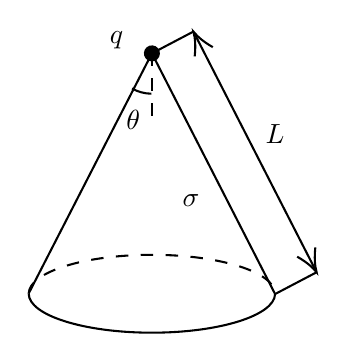
\begin{tikzpicture}[x=0.75pt,y=0.75pt,yscale=-1,xscale=1]
%uncomment if require: \path (0,179); %set diagram left start at 0, and has height of 179
%Shape: Arc [id:dp8722524247083157] 
\draw  [draw opacity=0] (404.7,143.06) .. controls (404.39,153.36) and (377.94,161.67) .. (345.35,161.67) .. controls (312.57,161.67) and (286,153.25) .. (286,142.88) .. controls (286,142.84) and (286,142.79) .. (286,142.75) -- (345.35,142.88) -- cycle ; \draw   (404.7,143.06) .. controls (404.39,153.36) and (377.94,161.67) .. (345.35,161.67) .. controls (312.57,161.67) and (286,153.25) .. (286,142.88) .. controls (286,142.84) and (286,142.79) .. (286,142.75) ;
%Straight Lines [id:da41562807214318487] 
\draw    (345.35,27.1) -- (286,142.75) ;
\draw [shift={(345.35,27.1)}, rotate = 117.17] [color={rgb, 255:red, 0; green, 0; blue, 0 }  ][fill={rgb, 255:red, 0; green, 0; blue, 0 }  ][line width=0.75]      (0, 0) circle [x radius= 3.35, y radius= 3.35]   ;
%Straight Lines [id:da0864473594730979] 
\draw    (345.35,27.1) -- (404.7,143.06) ;
%Shape: Arc [id:dp02270691632844124] 
\draw  [draw opacity=0][dash pattern={on 4.5pt off 4.5pt}] (286,142.75) .. controls (286.32,132.46) and (312.77,124.15) .. (345.35,124.15) .. controls (378.13,124.15) and (404.71,132.56) .. (404.71,142.94) .. controls (404.71,142.98) and (404.71,143.02) .. (404.7,143.06) -- (345.35,142.94) -- cycle ; \draw  [dash pattern={on 4.5pt off 4.5pt}] (286,142.75) .. controls (286.32,132.46) and (312.77,124.15) .. (345.35,124.15) .. controls (378.13,124.15) and (404.71,132.56) .. (404.71,142.94) .. controls (404.71,142.98) and (404.71,143.02) .. (404.7,143.06) ;
%Straight Lines [id:da5096097386774856] 
\draw    (366.27,18.38) -- (423.79,130.78) ;
\draw [shift={(424.7,132.56)}, rotate = 242.9] [color={rgb, 255:red, 0; green, 0; blue, 0 }  ][line width=0.75]    (10.93,-4.9) .. controls (6.95,-2.3) and (3.31,-0.67) .. (0,0) .. controls (3.31,0.67) and (6.95,2.3) .. (10.93,4.9)   ;
\draw [shift={(365.35,16.6)}, rotate = 62.9] [color={rgb, 255:red, 0; green, 0; blue, 0 }  ][line width=0.75]    (10.93,-4.9) .. controls (6.95,-2.3) and (3.31,-0.67) .. (0,0) .. controls (3.31,0.67) and (6.95,2.3) .. (10.93,4.9)   ;
%Straight Lines [id:da1951218082895887] 
\draw    (345.35,27.1) -- (365.35,16.6) ;
%Straight Lines [id:da0035881285174372834] 
\draw    (404.7,143.06) -- (424.7,132.56) ;
%Straight Lines [id:da09449695588845808] 
\draw  [dash pattern={on 4.5pt off 4.5pt}]  (345.35,27.1) -- (345.35,62.9) ;
%Shape: Arc [id:dp7273289513406822] 
\draw  [draw opacity=0] (345.11,46.54) .. controls (341.73,46.5) and (338.56,45.59) .. (335.8,44.04) -- (345.35,27.1) -- cycle ; \draw   (345.11,46.54) .. controls (341.73,46.5) and (338.56,45.59) .. (335.8,44.04) ;

% Text Node
\draw (331.6,53.22) node [anchor=north west][inner sep=0.75pt]    {$\theta $};
% Text Node
\draw (398.6,59.72) node [anchor=north west][inner sep=0.75pt]    {$L$};
% Text Node
\draw (358.6,93.72) node [anchor=north west][inner sep=0.75pt]    {$\sigma $};
% Text Node
\draw (323.6,15.22) node [anchor=north west][inner sep=0.75pt]    {$q$};
\end{tikzpicture}
        \end{center}
        \item Nếu mặt nón bị cắt ra làm đôi rồi ta bỏ đi nửa phía trên của mặt nón thì lực tác dụng lên điện tích $q$ do phần còn lại của mặt nón gây ra là bao nhiêu? Tìm góc $\theta$ để lực này đạt giá trị cực đại?
        \begin{center}
            
\tikzset{every picture/.style={line width=0.75pt}} %set default line width to 0.75pt        

\begin{tikzpicture}[x=0.75pt,y=0.75pt,yscale=-1,xscale=1]
%uncomment if require: \path (0,179); %set diagram left start at 0, and has height of 179

%Shape: Arc [id:dp8722524247083157] 
\draw  [draw opacity=0] (404.7,143.06) .. controls (404.39,153.36) and (377.94,161.67) .. (345.35,161.67) .. controls (312.57,161.67) and (286,153.25) .. (286,142.88) .. controls (286,142.84) and (286,142.79) .. (286,142.75) -- (345.35,142.88) -- cycle ; \draw   (404.7,143.06) .. controls (404.39,153.36) and (377.94,161.67) .. (345.35,161.67) .. controls (312.57,161.67) and (286,153.25) .. (286,142.88) .. controls (286,142.84) and (286,142.79) .. (286,142.75) ;
%Straight Lines [id:da41562807214318487] 
\draw  [dash pattern={on 4.5pt off 4.5pt}]  (345.35,27.1) -- (286,142.75) ;
\draw [shift={(345.35,27.1)}, rotate = 117.17] [color={rgb, 255:red, 0; green, 0; blue, 0 }  ][fill={rgb, 255:red, 0; green, 0; blue, 0 }  ][line width=0.75]      (0, 0) circle [x radius= 3.35, y radius= 3.35]   ;
%Straight Lines [id:da0864473594730979] 
\draw  [dash pattern={on 4.5pt off 4.5pt}]  (345.35,27.1) -- (404.7,143.06) ;
%Shape: Arc [id:dp02270691632844124] 
\draw  [draw opacity=0][dash pattern={on 4.5pt off 4.5pt}] (286,142.75) .. controls (286.32,132.46) and (312.77,124.15) .. (345.35,124.15) .. controls (378.13,124.15) and (404.71,132.56) .. (404.71,142.94) .. controls (404.71,142.98) and (404.71,143.02) .. (404.7,143.06) -- (345.35,142.94) -- cycle ; \draw  [dash pattern={on 4.5pt off 4.5pt}] (286,142.75) .. controls (286.32,132.46) and (312.77,124.15) .. (345.35,124.15) .. controls (378.13,124.15) and (404.71,132.56) .. (404.71,142.94) .. controls (404.71,142.98) and (404.71,143.02) .. (404.7,143.06) ;
%Straight Lines [id:da1951218082895887] 
\draw    (345.35,27.1) -- (365.35,16.6) ;
%Straight Lines [id:da0035881285174372834] 
\draw    (404.7,143.06) -- (424.7,132.56) ;
%Straight Lines [id:da09449695588845808] 
\draw  [dash pattern={on 4.5pt off 4.5pt}]  (345.35,27.1) -- (345.35,62.9) ;
%Shape: Arc [id:dp7273289513406822] 
\draw  [draw opacity=0] (345.11,46.54) .. controls (341.73,46.5) and (338.56,45.59) .. (335.8,44.04) -- (345.35,27.1) -- cycle ; \draw   (345.11,46.54) .. controls (341.73,46.5) and (338.56,45.59) .. (335.8,44.04) ;
%Straight Lines [id:da4468679529081703] 
\draw    (315.68,84.93) -- (286,142.75) ;
%Straight Lines [id:da535625430984253] 
\draw    (375.03,85.08) -- (404.7,143.06) ;
%Shape: Ellipse [id:dp07689204433200425] 
\draw   (315.68,84.93) .. controls (315.68,79.9) and (328.96,75.82) .. (345.35,75.82) .. controls (361.74,75.82) and (375.03,79.9) .. (375.03,84.93) .. controls (375.03,89.96) and (361.74,94.04) .. (345.35,94.04) .. controls (328.96,94.04) and (315.68,89.96) .. (315.68,84.93) -- cycle ;
%Straight Lines [id:da9727043166592628] 
\draw    (395.94,76.36) -- (423.79,130.78) ;
\draw [shift={(424.7,132.56)}, rotate = 242.9] [color={rgb, 255:red, 0; green, 0; blue, 0 }  ][line width=0.75]    (10.93,-4.9) .. controls (6.95,-2.3) and (3.31,-0.67) .. (0,0) .. controls (3.31,0.67) and (6.95,2.3) .. (10.93,4.9)   ;
\draw [shift={(395.03,74.58)}, rotate = 62.9] [color={rgb, 255:red, 0; green, 0; blue, 0 }  ][line width=0.75]    (10.93,-4.9) .. controls (6.95,-2.3) and (3.31,-0.67) .. (0,0) .. controls (3.31,0.67) and (6.95,2.3) .. (10.93,4.9)   ;
%Straight Lines [id:da4503631677459048] 
\draw    (375.03,84.93) -- (395.03,74.43) ;
%Straight Lines [id:da700649772483974] 
\draw    (366.27,18.23) -- (394.12,72.65) ;
\draw [shift={(395.03,74.43)}, rotate = 242.9] [color={rgb, 255:red, 0; green, 0; blue, 0 }  ][line width=0.75]    (10.93,-4.9) .. controls (6.95,-2.3) and (3.31,-0.67) .. (0,0) .. controls (3.31,0.67) and (6.95,2.3) .. (10.93,4.9)   ;
\draw [shift={(365.35,16.45)}, rotate = 62.9] [color={rgb, 255:red, 0; green, 0; blue, 0 }  ][line width=0.75]    (10.93,-4.9) .. controls (6.95,-2.3) and (3.31,-0.67) .. (0,0) .. controls (3.31,0.67) and (6.95,2.3) .. (10.93,4.9)   ;

% Text Node
\draw (331.6,53.22) node [anchor=north west][inner sep=0.75pt]    {$\theta $};
% Text Node
\draw (413.27,67.72) node [anchor=north west][inner sep=0.75pt]    {$\dfrac{L}{2}$};
% Text Node
\draw (358.6,93.72) node [anchor=north west][inner sep=0.75pt]    {$\sigma $};
% Text Node
\draw (323.6,15.22) node [anchor=north west][inner sep=0.75pt]    {$q$};
% Text Node
\draw (383.27,11.09) node [anchor=north west][inner sep=0.75pt]    {$\dfrac{L}{2}$};


\end{tikzpicture}

        \end{center}
    \end{enumerate} 
    \end{vd}
    \begin{loigiai}
        \begin{enumerate}[1)]
        \setlength{\itemsep}{0pt}
            \item 
            Xét một vòng nhỏ của mặt nón như hình. Khoảng cách từ một điểm trên vòng tới điện tích $q$ là $x$. Độ dày của vòng là $\dd x$, điện tích của vòng là $\dd Q$. Do tính đối xứng, lực do vòng này tác dụng lên điện tích $q$ có phương trùng với trục của hình nón.
            \begin{center}
                

\tikzset{every picture/.style={line width=0.75pt}} %set default line width to 0.75pt        

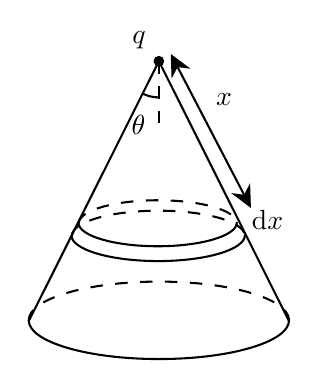
\begin{tikzpicture}[x=0.75pt,y=0.75pt,yscale=-1,xscale=1]
%uncomment if require: \path (0,379); %set diagram left start at 0, and has height of 379

%Shape: Boxed Line [id:dp22419819397820362] 
\draw    (388.71,190) -- (326,64.73) ;
%Shape: Boxed Line [id:dp8361374790173637] 
\draw    (326,64.73) -- (263.29,190) ;
%Shape: Arc [id:dp8323260940556365] 
\draw  [draw opacity=0][dash pattern={on 4.5pt off 4.5pt}] (263.29,190) .. controls (263.28,189.87) and (263.28,189.73) .. (263.28,189.6) .. controls (263.28,179.29) and (291.35,170.94) .. (325.99,170.94) .. controls (360.25,170.94) and (388.1,179.11) .. (388.69,189.27) -- (325.99,189.6) -- cycle ; \draw  [dash pattern={on 4.5pt off 4.5pt}] (263.29,190) .. controls (263.28,189.87) and (263.28,189.73) .. (263.28,189.6) .. controls (263.28,179.29) and (291.35,170.94) .. (325.99,170.94) .. controls (360.25,170.94) and (388.1,179.11) .. (388.69,189.27) ;
%Shape: Arc [id:dp14495509734027934] 
\draw  [draw opacity=0] (388.68,189.19) .. controls (388.69,189.32) and (388.7,189.46) .. (388.7,189.6) .. controls (388.7,199.9) and (360.62,208.25) .. (325.99,208.25) .. controls (291.72,208.25) and (263.88,200.08) .. (263.29,189.92) -- (325.99,189.6) -- cycle ; \draw   (388.68,189.19) .. controls (388.69,189.32) and (388.7,189.46) .. (388.7,189.6) .. controls (388.7,199.9) and (360.62,208.25) .. (325.99,208.25) .. controls (291.72,208.25) and (263.88,200.08) .. (263.29,189.92) ;
%Flowchart: Connector [id:dp6307334720269582] 
\draw  [fill={rgb, 255:red, 0; green, 0; blue, 0 }  ,fill opacity=1 ] (328.04,64.73) .. controls (328.04,63.6) and (327.13,62.69) .. (326,62.69) .. controls (324.87,62.69) and (323.96,63.6) .. (323.96,64.73) .. controls (323.96,65.85) and (324.87,66.77) .. (326,66.77) .. controls (327.13,66.77) and (328.04,65.85) .. (328.04,64.73) -- cycle ;
%Shape: Arc [id:dp275573446352523] 
\draw  [draw opacity=0] (363.52,142.31) .. controls (363.52,142.4) and (363.53,142.48) .. (363.53,142.56) .. controls (363.53,148.83) and (346.45,153.91) .. (325.38,153.91) .. controls (304.54,153.91) and (287.6,148.94) .. (287.24,142.76) -- (325.38,142.56) -- cycle ; \draw   (363.52,142.31) .. controls (363.52,142.4) and (363.53,142.48) .. (363.53,142.56) .. controls (363.53,148.83) and (346.45,153.91) .. (325.38,153.91) .. controls (304.54,153.91) and (287.6,148.94) .. (287.24,142.76) ;
%Shape: Arc [id:dp8384783979328538] 
\draw  [draw opacity=0][dash pattern={on 4.5pt off 4.5pt}] (287.44,143.04) .. controls (287.43,142.96) and (287.43,142.88) .. (287.43,142.79) .. controls (287.43,136.69) and (304.46,131.75) .. (325.48,131.75) .. controls (346.26,131.75) and (363.15,136.59) .. (363.52,142.59) -- (325.48,142.79) -- cycle ; \draw  [dash pattern={on 4.5pt off 4.5pt}] (287.44,143.04) .. controls (287.43,142.96) and (287.43,142.88) .. (287.43,142.79) .. controls (287.43,136.69) and (304.46,131.75) .. (325.48,131.75) .. controls (346.26,131.75) and (363.15,136.59) .. (363.52,142.59) ;

%Shape: Arc [id:dp8765623300384509] 
\draw  [draw opacity=0] (367.42,148.35) .. controls (367.42,148.44) and (367.43,148.53) .. (367.43,148.62) .. controls (367.43,155.48) and (348.71,161.05) .. (325.63,161.05) .. controls (302.79,161.05) and (284.23,155.6) .. (283.84,148.84) -- (325.63,148.62) -- cycle ; \draw   (367.42,148.35) .. controls (367.42,148.44) and (367.43,148.53) .. (367.43,148.62) .. controls (367.43,155.48) and (348.71,161.05) .. (325.63,161.05) .. controls (302.79,161.05) and (284.23,155.6) .. (283.84,148.84) ;
%Shape: Arc [id:dp5737904793381008] 
\draw  [draw opacity=0][dash pattern={on 4.5pt off 4.5pt}] (284.06,149.14) .. controls (284.05,149.05) and (284.05,148.96) .. (284.05,148.87) .. controls (284.05,142.19) and (302.71,136.77) .. (325.74,136.77) .. controls (348.51,136.77) and (367.01,142.07) .. (367.42,148.66) -- (325.74,148.87) -- cycle ; \draw  [dash pattern={on 4.5pt off 4.5pt}] (284.06,149.14) .. controls (284.05,149.05) and (284.05,148.96) .. (284.05,148.87) .. controls (284.05,142.19) and (302.71,136.77) .. (325.74,136.77) .. controls (348.51,136.77) and (367.01,142.07) .. (367.42,148.66) ;

%Straight Lines [id:da43845242333776446] 
\draw  [dash pattern={on 4.5pt off 4.5pt}]  (326,64.73) -- (326,96.33) ;
%Shape: Arc [id:dp5839079332046728] 
\draw  [draw opacity=0] (318.06,80.3) .. controls (320.42,81.51) and (323.1,82.19) .. (325.93,82.2) -- (326,64.73) -- cycle ; \draw   (318.06,80.3) .. controls (320.42,81.51) and (323.1,82.19) .. (325.93,82.2) ;
%Straight Lines [id:da29622780840372] 
\draw    (333.11,63.92) -- (368.94,132.76) ;
\draw [shift={(370.33,135.42)}, rotate = 242.5] [fill={rgb, 255:red, 0; green, 0; blue, 0 }  ][line width=0.08]  [draw opacity=0] (10.72,-5.15) -- (0,0) -- (10.72,5.15) -- (7.12,0) -- cycle    ;
\draw [shift={(331.72,61.26)}, rotate = 62.5] [fill={rgb, 255:red, 0; green, 0; blue, 0 }  ][line width=0.08]  [draw opacity=0] (10.72,-5.15) -- (0,0) -- (10.72,5.15) -- (7.12,0) -- cycle    ;

% Text Node
\draw (311.32,89.1) node [anchor=north west][inner sep=0.75pt]    {$\theta $};
% Text Node
\draw (311.72,49.1) node [anchor=north west][inner sep=0.75pt]    {$q$};
% Text Node
\draw (352.12,78.62) node [anchor=north west][inner sep=0.75pt]    {$x$};
% Text Node
\draw (369.32,135.26) node [anchor=north west][inner sep=0.75pt]    {$\mathrm{d} x$};
\end{tikzpicture}

            \end{center}
            Lực do vòng tác dụng lên điện tích $q$ là:
            \[\dd F=\dfrac{q(\dd Q)\cos\theta}{4\pi \varepsilon_0 x^2}. \tag{1}  \label{ca1}\]
            Bán kính của vòng là $x\sin\theta$, diện tích của vòng sẽ là $2\pi(x\sin\theta) \dd x $. Điện tích của vòng là $\dd Q=\sigma 2\pi(x\sin\theta) \dd x$. Tích phân (\ref{ca1}) lấy cận từ $x=0$ tới $x=L$, ta có:
            \begin{equation*}
                F=\tiph{0}{L}{\dfrac{q\tron{\sigma 2\pi x\sin\theta}\cos\theta}{4\pi \varepsilon_0 x^2}}{x}=\dfrac{q\sigma \sin\theta\cos\theta}{2\varepsilon_0}\int_0^L\dfrac{\dd x}{x}.
            \end{equation*}
            Tích phân này phân kì, lực tác dụng lên điện tích $q$ là vô cùng lớn. 
            \item Bây giờ ta lại tính tích phân (\ref{ca1}) nhưng lấy cận từ $x=\dfrac{L}{2}$ đến $x=L$:
            \begin{equation*}
            \begin{aligned}
               F&=\tiph{\frac{L}{2}}{L}{\dfrac{q\tron{\sigma 2\pi x\sin\theta}\cos\theta}{4\pi \varepsilon_0 x^2}}{x}\\
               &=\dfrac{q\sigma \sin\theta\cos\theta}{2\varepsilon_0}\int_\frac{L}{2}^L\dfrac{\dd x}{x}\\
               &=\dfrac{q\sigma \sin\theta\cos\theta}{2\varepsilon_0}\ln 2.
            \end{aligned}
            \end{equation*}
            Ta có $\sin \theta \cos \theta=\dfrac{1}{2}\sin2\theta$, lực tác dụng lên điện tích $q$ cực đại khi $2\theta=90^\circ\Rightarrow\theta=45^\circ$. Khi đó lực tác dụng lên $q$ có giá trị là $F=\dfrac{q\sigma\ln 2}{4\varepsilon_0}$. Ta thấy rằng khi $\theta=90^\circ$ thì lực tác dụng lên điện tích bằng không, trường hợp này tương đương với việc điện tích ở giữa một lỗ tròn trên một vành tròn. Lực cũng bằng không khi $\theta=0^\circ$, trường hợp này tương đương với một mặt nón hẹp vô cùng. \\
            Lưu ý rằng lực tác dụng lên điện tích không phụ thuộc vào $L$. Điều này là do khi ta tăng kích thước của hình nón lên 5 lần, diện tích mặt nón tăng 25 lần và do đó điện tích trên mặt nón cũng tăng 25 lần. Tuy nhiên, khoảng cách từ mặt nón đến điện tích cũng tăng 5 lần và lực tỉ lệ nghịch với khoảng cách bình phương nên kết quả là lực không đổi.
        \end{enumerate}
    \end{loigiai}
    \renewcommand{\theequation}{\arabic{equation}}
    
    
     \begin{vd}[Điện trường của một chiếc vỏ bán cầu]
    Một chiếc vỏ hình bán cầu với bán kính $R$ được tích điện đều với mật độ điện mặt $\sigma$. Tìm điện trường tại một điểm nằm trên trục đối xứng của lớp vỏ, cách tâm của hình bán cầu một khoảng là $z$ ($z$ có giá trị bất kì từ $-\infty$ đến $\infty$).
    \end{vd}
    \begin{loigiai}
        Xét một vòng nhỏ thuộc mặt bán cầu như hình vẽ. Diện tích của vòng này là $2\pi (R\sin\theta)(R\dd \theta)$, điện tích của vòng sẽ là $\sigma\tron{2\pi R^2\sin\theta\dd \theta}$. 
        \begin{center}
            

\tikzset{every picture/.style={line width=0.75pt}} %set default line width to 0.75pt        

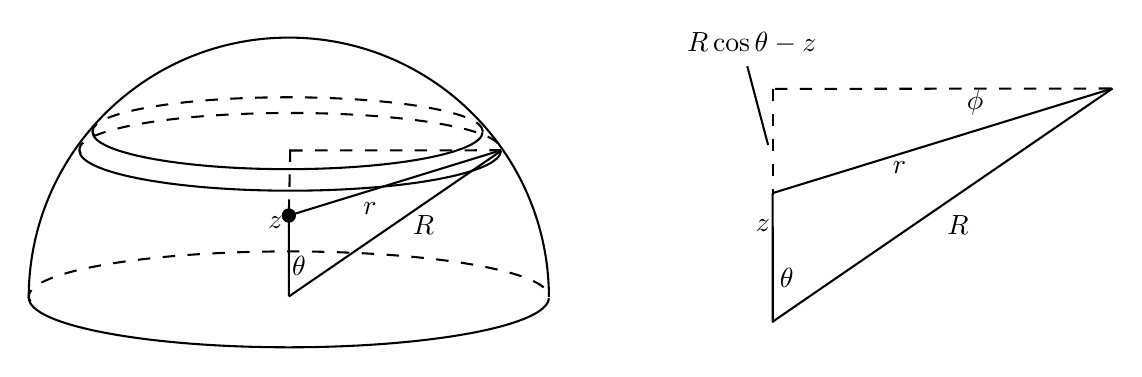
\begin{tikzpicture}[x=0.75pt,y=0.75pt,yscale=-1,xscale=1]
%uncomment if require: \path (0,238); %set diagram left start at 0, and has height of 238

%Shape: Arc [id:dp46202423649235325] 
\draw  [draw opacity=0] (100.97,186.37) .. controls (100.97,186.26) and (100.97,186.15) .. (100.97,186.04) .. controls (100.97,116.83) and (157.08,60.73) .. (226.29,60.73) .. controls (295.41,60.73) and (351.45,116.68) .. (351.61,185.76) -- (226.29,186.04) -- cycle ; \draw   (100.97,186.37) .. controls (100.97,186.26) and (100.97,186.15) .. (100.97,186.04) .. controls (100.97,116.83) and (157.08,60.73) .. (226.29,60.73) .. controls (295.41,60.73) and (351.45,116.68) .. (351.61,185.76) ;
%Shape: Arc [id:dp1474574470654193] 
\draw  [draw opacity=0] (351.57,186.3) .. controls (350.83,199.38) and (295.02,209.94) .. (226.29,209.94) .. controls (157.1,209.94) and (101,199.24) .. (101,186.04) .. controls (101,185.95) and (101.01,185.87) .. (101.01,185.78) -- (226.29,186.04) -- cycle ; \draw   (351.57,186.3) .. controls (350.83,199.38) and (295.02,209.94) .. (226.29,209.94) .. controls (157.1,209.94) and (101,199.24) .. (101,186.04) .. controls (101,185.95) and (101.01,185.87) .. (101.01,185.78) ;
%Shape: Arc [id:dp4891947324082879] 
\draw  [draw opacity=0][dash pattern={on 4.5pt off 4.5pt}] (101.83,187.91) .. controls (101.31,187.1) and (101.04,186.28) .. (101.04,185.45) .. controls (101.04,173.47) and (157.13,163.75) .. (226.33,163.75) .. controls (295.52,163.75) and (351.61,173.47) .. (351.61,185.45) .. controls (351.61,185.6) and (351.6,185.76) .. (351.59,185.91) -- (226.33,185.45) -- cycle ; \draw  [dash pattern={on 4.5pt off 4.5pt}] (101.83,187.91) .. controls (101.31,187.1) and (101.04,186.28) .. (101.04,185.45) .. controls (101.04,173.47) and (157.13,163.75) .. (226.33,163.75) .. controls (295.52,163.75) and (351.61,173.47) .. (351.61,185.45) .. controls (351.61,185.6) and (351.6,185.76) .. (351.59,185.91) ;

%Shape: Arc [id:dp5026419323128228] 
\draw  [draw opacity=0] (319.65,106.4) .. controls (319.1,116.2) and (277.24,124.12) .. (225.69,124.12) .. controls (173.79,124.12) and (131.71,116.1) .. (131.71,106.2) .. controls (131.71,106.13) and (131.71,106.07) .. (131.72,106) -- (225.69,106.2) -- cycle ; \draw   (319.65,106.4) .. controls (319.1,116.2) and (277.24,124.12) .. (225.69,124.12) .. controls (173.79,124.12) and (131.71,116.1) .. (131.71,106.2) .. controls (131.71,106.13) and (131.71,106.07) .. (131.72,106) ;
%Shape: Arc [id:dp7452969809878249] 
\draw  [draw opacity=0][dash pattern={on 4.5pt off 4.5pt}] (132.33,107.6) .. controls (131.94,106.99) and (131.74,106.38) .. (131.74,105.76) .. controls (131.74,96.77) and (173.81,89.48) .. (225.71,89.48) .. controls (277.61,89.48) and (319.69,96.77) .. (319.69,105.76) .. controls (319.69,105.87) and (319.68,105.99) .. (319.67,106.1) -- (225.71,105.76) -- cycle ; \draw  [dash pattern={on 4.5pt off 4.5pt}] (132.33,107.6) .. controls (131.94,106.99) and (131.74,106.38) .. (131.74,105.76) .. controls (131.74,96.77) and (173.81,89.48) .. (225.71,89.48) .. controls (277.61,89.48) and (319.69,96.77) .. (319.69,105.76) .. controls (319.69,105.87) and (319.68,105.99) .. (319.67,106.1) ;

%Shape: Arc [id:dp6482262977695161] 
\draw  [draw opacity=0] (328.52,115.33) .. controls (327.92,125.93) and (282.67,134.49) .. (226.94,134.49) .. controls (170.84,134.49) and (125.36,125.82) .. (125.36,115.12) .. controls (125.36,115.05) and (125.36,114.98) .. (125.37,114.9) -- (226.94,115.12) -- cycle ; \draw   (328.52,115.33) .. controls (327.92,125.93) and (282.67,134.49) .. (226.94,134.49) .. controls (170.84,134.49) and (125.36,125.82) .. (125.36,115.12) .. controls (125.36,115.05) and (125.36,114.98) .. (125.37,114.9) ;
%Shape: Arc [id:dp5722220594040952] 
\draw  [draw opacity=0][dash pattern={on 4.5pt off 4.5pt}] (126.04,116.63) .. controls (125.61,115.98) and (125.39,115.31) .. (125.39,114.64) .. controls (125.39,104.92) and (170.87,97.04) .. (226.97,97.04) .. controls (283.08,97.04) and (328.56,104.92) .. (328.56,114.64) .. controls (328.56,114.76) and (328.55,114.89) .. (328.53,115.01) -- (226.97,114.64) -- cycle ; \draw  [dash pattern={on 4.5pt off 4.5pt}] (126.04,116.63) .. controls (125.61,115.98) and (125.39,115.31) .. (125.39,114.64) .. controls (125.39,104.92) and (170.87,97.04) .. (226.97,97.04) .. controls (283.08,97.04) and (328.56,104.92) .. (328.56,114.64) .. controls (328.56,114.76) and (328.55,114.89) .. (328.53,115.01) ;

%Shape: Circle [id:dp8026705426471774] 
\draw  [fill={rgb, 255:red, 0; green, 0; blue, 0 }  ,fill opacity=1 ] (223.35,146.48) .. controls (223.35,144.86) and (224.67,143.54) .. (226.29,143.54) .. controls (227.91,143.54) and (229.23,144.86) .. (229.23,146.48) .. controls (229.23,148.1) and (227.91,149.41) .. (226.29,149.41) .. controls (224.67,149.41) and (223.35,148.1) .. (223.35,146.48) -- cycle ;
%Straight Lines [id:da5877503000958018] 
\draw    (328.52,115.33) -- (226.33,185.45) ;
%Straight Lines [id:da9071270274301693] 
\draw    (226.29,146.48) -- (226.33,185.45) ;
%Straight Lines [id:da2538994438706397] 
\draw    (226.29,146.48) -- (328.53,115.01) ;
%Straight Lines [id:da1316663756659071] 
\draw  [dash pattern={on 4.5pt off 4.5pt}]  (226.97,114.64) -- (226.29,146.48) ;
%Straight Lines [id:da792894079434711] 
\draw  [dash pattern={on 4.5pt off 4.5pt}]  (226.94,115.12) -- (328.53,115.01) ;
%Straight Lines [id:da007313747973220375] 
\draw    (623.11,85.26) -- (459.49,197.54) ;
%Straight Lines [id:da7788416655056725] 
\draw    (459.41,135.65) -- (623.11,85.26) ;
%Straight Lines [id:da6146780143403707] 
\draw    (459.41,135.65) -- (459.46,198.05) ;
%Straight Lines [id:da6887305258581999] 
\draw  [dash pattern={on 4.5pt off 4.5pt}]  (459.45,85.44) -- (459.45,136.41) ;
%Straight Lines [id:da31195822900542547] 
\draw  [dash pattern={on 4.5pt off 4.5pt}]  (460.45,85.44) -- (623.11,85.26) ;
%Straight Lines [id:da2917501321835787] 
\draw    (447.17,74.5) -- (457.21,112.48) ;

% Text Node
\draw (226.39,164.4) node [anchor=north west][inner sep=0.75pt]    {$\theta $};
% Text Node
\draw (284.51,144.76) node [anchor=north west][inner sep=0.75pt]    {$R$};
% Text Node
\draw (260.66,138.75) node [anchor=north west][inner sep=0.75pt]    {$r$};
% Text Node
\draw (214.98,145.51) node [anchor=north west][inner sep=0.75pt]    {$z$};
% Text Node
\draw (542.14,144.81) node [anchor=north west][inner sep=0.75pt]    {$R$};
% Text Node
\draw (515.86,119.1) node [anchor=north west][inner sep=0.75pt]    {$r$};
% Text Node
\draw (461.43,170.25) node [anchor=north west][inner sep=0.75pt]    {$\theta $};
% Text Node
\draw (449.76,146.98) node [anchor=north west][inner sep=0.75pt]    {$z$};
% Text Node
\draw (551.48,84.5) node [anchor=north west][inner sep=0.75pt]    {$\phi $};
% Text Node
\draw (416.75,56.45) node [anchor=north west][inner sep=0.75pt]    {$R\cos \theta -z$};


\end{tikzpicture}

        \end{center}
        Từ hình ta có $r=\sqrt{R^2+z^2-2Rz\cos\theta}$ và $\sin\phi=\dfrac{R\cos\theta-z}{r}$. Do tính đối xứng, điện trường do vòng gây ra hướng dọc theo trục đối xứng của hệ. Điện trường gây ra bởi vòng tại một điểm trên trục $z$ là:
        \begin{equation}
            \begin{aligned}
               \dd E_z&=-\dfrac{\sigma\tron{2\pi R^2\sin\theta\dd \theta}}{4\pi \varepsilon_0 r^2}\sin\phi\\
               &=-\dfrac{\sigma\tron{2\pi R^2\sin\theta\dd \theta}}{4\pi \varepsilon_0 \tron{R^2+z^2-2Rz\cos\theta}}\dfrac{R\cos\theta-z}{\sqrt{R^2+z^2-2Rz\cos\theta}}\\
               &=-\dfrac{\sigma R^2}{2 \varepsilon_0}\dfrac{\sin \theta\tron{R\cos\theta-z}\dd\theta}{\tron{R^2+z^2-2Rz\cos\theta}^{\frac{3}{2}}}.
            \end{aligned}
            \label{ca2}
        \end{equation}
        Tích phân (\ref{ca2}) lấy cận từ $\theta=0$ đến $\theta=\dfrac{\pi}{2}$ ta được điện trường gây ra bởi cả vỏ bán cầu:
        \begin{equation}
            E(z)=-\dfrac{\sigma R^2}{2 \varepsilon_0}\tiph{0}{\textstyle\frac{\pi}{2}}{\dfrac{\sin \theta\tron{R\cos\theta-z}}{\tron{R^2+z^2-2Rz\cos\theta}^{\frac{3}{2}}}}{\theta}.
        \end{equation}
        Tích phân này có thể được biểu diễn bằng hàm sơ cấp, cụ thể:
        \begin{equation}
            \int \dfrac{\sin x(a\cos x-b)\dd x}{\tron{a^2+b^2-2ab\cos x}^{\frac{3}{2}}}=\dfrac{-a+b\cos x}{b^2\sqrt{a^2+b^2-2ab\cos x}}.
        \end{equation}
        Từ đó, ta có:
        \begin{equation}
        \begin{aligned}
           E(z)&=\dfrac{\sigma R^2}{2\varepsilon_0}\left.\dfrac{R-z\cos\theta}{z^2\sqrt{R^2+z^2-2Rz\cos\theta}}\right|_0^{\textstyle\frac{\pi}{2}}\\
           &=\dfrac{\sigma R^2}{2\varepsilon_0 z^2}\tron{\dfrac{R}{\sqrt{R^2+z^2}}-\dfrac{R-z}{\sqrt{(R-z)^2}}}.
        \end{aligned}
        \end{equation}
        Ta có:
        \begin{equation}
            \begin{aligned}
               &E(z)=\dfrac{\sigma R^2}{2\varepsilon_0 z^2}\tron{\dfrac{1}{\sqrt{1+\dfrac{z^2}{R^2}}}-1}\ \text{với} \ z<R,\\
               &E(z)=\dfrac{\sigma R^2}{2\varepsilon_0 z^2}\tron{\dfrac{1}{\sqrt{1+\dfrac{z^2}{R^2}}}+1}\ \text{với}\ z>R.
            \end{aligned}
        \end{equation}
        Khi $z<R$ thì $E(z)<0$, chứng tỏ điện trường luôn hướng xuống dưới. Điều này là dễ thấy với những điểm nằm bên dưới vỏ bán cầu, nhưng đối với những điểm nằm bên trong vỏ thì không. Đối với những điểm $z>R$ thì $E(z)>0$, điện trường luôn hướng lên trên, điều này là dễ thấy. Ta nhận thấy hàm $E(z)$ là một hàm không liên tục, đứt đoạn tại $z=R$. Tại đây điện trường đột ngột thay đổi một khoảng $\dfrac{\sigma}{\varepsilon_0}$, ta có thể thấy kết quả trên đồng nhất với định luật Gauss khi xét một mặt Gauss hình trụ nhỏ tại đỉnh của chiếc vỏ bán cầu.\\
        Điện tích của vỏ cầu là $Q=2\pi R^2 \sigma$. Khi $z\gg R$, ta thấy $E(z)\approx\dfrac{Q}{4\pi\varepsilon_0z^2}$ (chiếc vỏ bán cầu giống như một điện tích điểm $Q$ khi $z\gg R$).\\
        Khi $z\rightarrow 0$, ta có thể sử dụng công thức tính gần đúng $\dfrac{1}{\sqrt{1+\epsilon}}\approx 1-\dfrac{\epsilon}{2}$.\\
        Ta tính được điện trường tại tâm của vỏ bán cầu là $E(0)=-\dfrac{\sigma}{4\varepsilon_0}=-\dfrac{Q}{8\pi\varepsilon_0R^2}$. Điện trường này bằng một nửa so với điện trường của một mặt phẳng vô hạn tích điện đều $\dfrac{\sigma}{2\varepsilon_0}$. \\
        Ta cũng có thể nhận thấy rằng trong khoảng $-R<z<R$ thì $E(z)$ là một hàm chẵn, tức là $E(z)=E(-z)$. Điều này có thể được lí giải như sau: Tưởng tượng ta có một vỏ bán cầu y hệt và ta ghép hai vỏ lại với nhau, hệ lúc này như một vỏ cầu tích điện đều và điện trường bên trong bằng không, từ đó suy ra được cường điện trường do hai vỏ phải gây ra tại một điểm bằng nhau và ngược chiều.
    \end{loigiai}
    
    
    \begin{vd}[Điện trường ``đều'']
    \begin{enumerate}[1)]
        \setlength{\itemsep}{0pt}
        \item Hai vòng giống nhau có bán kính $r$ được tích điện đều trái dấu với điện tích $Q$ và $-Q$. Hai vòng dược đặt song song đồng trục với nhau và cách nhau một khoảng là $h$. Chọn hệ trục tọa độ sao cho gốc $O$ trùng với tâm vòng tròn dưới và trục $Oz$ hướng thẳng đứng lên trên như hình. Tìm điện trường tại một điểm trên trục đối xứng như là một hàm của tọa độ $z$ của điểm đó.
        \begin{center}
            

\tikzset{every picture/.style={line width=0.75pt}} %set default line width to 0.75pt        

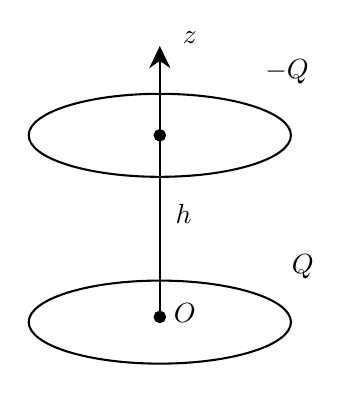
\begin{tikzpicture}[x=0.75pt,y=0.75pt,yscale=-1,xscale=1]
%uncomment if require: \path (0,300); %set diagram left start at 0, and has height of 300

%Shape: Ellipse [id:dp2611977812107278] 
\draw   (238.67,103.33) .. controls (238.67,92.29) and (266.95,83.33) .. (301.83,83.33) .. controls (336.72,83.33) and (365,92.29) .. (365,103.33) .. controls (365,114.38) and (336.72,123.33) .. (301.83,123.33) .. controls (266.95,123.33) and (238.67,114.38) .. (238.67,103.33) -- cycle ;
%Shape: Ellipse [id:dp11508494117645407] 
\draw   (238.67,193.33) .. controls (238.67,182.29) and (266.95,173.33) .. (301.83,173.33) .. controls (336.72,173.33) and (365,182.29) .. (365,193.33) .. controls (365,204.38) and (336.72,213.33) .. (301.83,213.33) .. controls (266.95,213.33) and (238.67,204.38) .. (238.67,193.33) -- cycle ;
%Straight Lines [id:da37645034409859846] 
\draw    (301.83,193.33) -- (301.83,63.33) ;
\draw [shift={(301.83,60.33)}, rotate = 450] [fill={rgb, 255:red, 0; green, 0; blue, 0 }  ][line width=0.08]  [draw opacity=0] (10.72,-5.15) -- (0,0) -- (10.72,5.15) -- (7.12,0) -- cycle    ;
%Shape: Circle [id:dp1214444367479659] 
\draw  [fill={rgb, 255:red, 0; green, 0; blue, 0 }  ,fill opacity=1 ] (299.33,190.83) .. controls (299.33,189.45) and (300.45,188.33) .. (301.83,188.33) .. controls (303.21,188.33) and (304.33,189.45) .. (304.33,190.83) .. controls (304.33,192.21) and (303.21,193.33) .. (301.83,193.33) .. controls (300.45,193.33) and (299.33,192.21) .. (299.33,190.83) -- cycle ;
%Shape: Circle [id:dp06318371813380885] 
\draw  [fill={rgb, 255:red, 0; green, 0; blue, 0 }  ,fill opacity=1 ] (299.33,103.33) .. controls (299.33,101.95) and (300.45,100.83) .. (301.83,100.83) .. controls (303.21,100.83) and (304.33,101.95) .. (304.33,103.33) .. controls (304.33,104.71) and (303.21,105.83) .. (301.83,105.83) .. controls (300.45,105.83) and (299.33,104.71) .. (299.33,103.33) -- cycle ;

% Text Node
\draw (307.14,183.11) node [anchor=north west][inner sep=0.75pt]    {$O$};
% Text Node
\draw (311.43,51.97) node [anchor=north west][inner sep=0.75pt]    {$z$};
% Text Node
\draw (351.14,65.11) node [anchor=north west][inner sep=0.75pt]    {$-Q$};
% Text Node
\draw (364,159.26) node [anchor=north west][inner sep=0.75pt]    {$Q$};
% Text Node
\draw (308,135.26) node [anchor=north west][inner sep=0.75pt]    {$h$};


\end{tikzpicture}

        \end{center}
        \item Bạn sẽ thấy điện trường trên trục đối xứng là một hàm đối xứng qua điểm có $z=\dfrac{h}{2}$. Điều đó chứng tỏ rằng tại đây thì điện trường đạt cực trị. Và cũng tại điểm này thì điện trường tương đối ``đều'', đạo hàm bậc nhất của điện trường theo tọa độ tại điểm này bằng không. Tìm $r$ theo $h$ để điện trường là ``rất đều'', tức là đạo hàm bậc hai của điện trường theo tọa độ cũng bằng không. Bạn có thể sử dụng sự hỗ trợ của máy tính.
    \end{enumerate}
    \end{vd}
     \begin{loigiai}
        \begin{enumerate}[1)]
        \setlength{\itemsep}{0pt}
            \item Tại điểm có độ cao $z$ phía trên vòng dưới, điện trường gây ra bởi một điện tích $\dd Q$ nằm trên vòng dưới là $\dfrac{\dd Q}{4\pi\varepsilon_0\tron{r^2+z^2}}$. Nhưng do tính đối xứng của hệ, điện trường tổng hợp tại điểm đó có phương trùng với trục đối xứng của hệ, vậy nên chỉ có thành phần điện trường theo trục $z$ do $\dd Q$ gây ra mới đóng góp vào điện trường tổng hợp, vì thế ta phải nhân thêm một hệ số $\dfrac{z}{\sqrt{r^2+z^2}}$. Điện trường do vòng dưới gây ra tại điểm trên trục có tọa độ $z$ là:
            \begin{equation}
                E_d(z)=\dfrac{Qz}{4\pi\varepsilon_0\tron{r^2+z^2}^{\frac{3}{2}}}.
            \end{equation}
            Tương tự với vòng phía trên, điện trường do vòng này gây ra là:
            \begin{equation}
                 E_u(z)=\dfrac{Q(h-z)}{4\pi\varepsilon_0\tron{r^2+\tron{h-z}^2}^{\frac{3}{2}}}.
            \end{equation}
             Điện trường tổng hợp tại điểm có tọa độ $z$:
        \begin{equation}
            E(z)=\dfrac{Q}{4\pi\varepsilon_0}\tron{\dfrac{z}{\tron{r^2+z^2}^{\frac{3}{2}}}+\dfrac{h-z}{\tron{r^2+\tron{h-z}^2}^{\frac{3}{2}}}}.
        \end{equation}
            \item Ta thấy biểu thức $E(z)$ không thay đổi nếu ta thay $z$ bằng $h-z$. Nếu ta đặt $z'=z-\dfrac{h}{z}$ là tọa độ của điểm cần tính so với gốc là trung điểm của đoạn nối tâm hai vòng, thì khi ta thay $z'$ bằng $(h-z)-\dfrac{h}{2}=-z'$ thì điện trường không thay đổi. Điều nay có nghĩa là $E(z')$ là một hàm chẵn. Vậy nên điện trường đối xứng qua mặt phẳng $z=\dfrac{h}{2}$, giống như dự đoán. Do đó cường độ điện trường đạt cực trị tại vị trí $z=\dfrac{h}{2}$. \\
            Ta có:
            \begin{equation}
            \begin{aligned}
               &E(z)=\dfrac{Q}{4\pi\varepsilon_0}\tron{\dfrac{z}{\tron{r^2+z^2}^{\frac{3}{2}}}+\dfrac{h-z}{\tron{r^2+\tron{h-z}^2}^{\frac{3}{2}}}},\\
               &\begin{aligned}
                  \dfrac{\dd E}{\dd z}=\dfrac{Q}{4\pi \varepsilon_0}\left(\rule{0cm}{0.9cm} \right.&\dfrac{\tron{r^2+z^2}^\frac{3}{2}-3z^2\tron{r^2+z^2}^\frac{3}{2}}{\tron{r^2+z^2}^3}\\
                  &\left. +\dfrac{-\tron{r^2+\tron{h-z}^2}^\frac{3}{2}+3\tron{h-z}^2\tron{r^2+\tron{h-z}^2}}{\tron{r^2\tron{h-z}^2}^3}\right),
               \end{aligned}\\
               &\begin{aligned}
                  \dfrac{\dd^2 E}{\dd z^2}=\dfrac{Q}{4\pi \varepsilon_0}\left(\rule{0cm}{0.9cm}\right.\dfrac{15z^3}{\tron{r^2+z^2}^\frac{7}{2}}&-\dfrac{9z}{\tron{r^2+z^2}^\frac{5}{2}}\\
                &\left.+\dfrac{15\tron{h-z}^3}{\tron{r^2+\tron{h-z}^2}^\frac{7}{2}}-\dfrac{9\tron{h-z}}{\tron{r^2+\tron{h-z}^2}^\frac{5}{2}}\right).
               \end{aligned}
               \label{ca3}
            \end{aligned}
            \end{equation}
            Thay $z=\dfrac{h}{2}$ vào (\ref{ca3}), ta có:
            \begin{equation}
                \begin{aligned}
                  \left .\dfrac{\dd^2 E}{\dd z^2}\right|_{z=\frac{h}{2}}=\dfrac{Q}{2\pi \varepsilon_0}\tron{\dfrac{15h^3}{8\tron{r^2+\dfrac{h^2}{4}}^\frac{7}{2}}-\dfrac{9h}{2\tron{r^2+\dfrac{h^2}{4}}^\frac{5}{2}}}.
               \end{aligned}
            \end{equation}
            Để cho điện trường tại $z=\dfrac{h}{2}$ là ``rất đều'', đạo hàm bậc hai của cường độ điện trường tại đó phải bằng không. Ta có:
            \begin{equation}
                \begin{aligned}
                     \left . \dfrac{\dd^2 E}{\dd z^2}\right|_{z=\frac{h}{2}}=0&\Leftrightarrow \dfrac{15h^3}{8\tron{r^2+\dfrac{h^2}{4}}^\frac{7}{2}}-\dfrac{9h}{2\tron{r^2+\dfrac{h^2}{4}}^\frac{5}{2}}=0\\
                     &\Leftrightarrow \dfrac{15h^2}{8\left(r^2+\dfrac{h^2}{4}\right)}-\dfrac{9}{2}=0\\
                     &\Leftrightarrow r=\dfrac{h}{\sqrt{6}}\approx 0,41h.
                \end{aligned}
            \end{equation}
            Vậy để điện trường tại trung điểm của đường nối tâm hai vòng dây là rất đều thì đường kính của các vòng phải bằng khoảng 0,82 lần khoảng cách giữa các vòng. Đồ thị của $E(z)$ với các giá trị $r$ khác nhau được cho hình dưới. Trên đồ thị, điện trường được tính theo đơn vị $\dfrac{Q}{4\pi \varepsilon_0 h^2}$. Tại $r=\dfrac{h}{\sqrt{6}}$ thì cường độ điện trường tại vị trí $z=\dfrac{h}{2}$  chuyển từ cực tiểu sang cực đại. Với giá trị $r\ll h$ thì điện trường gần các vòng là rất lớn, giống như điện trường gây bởi các điện tích điểm.
            \begin{center}
                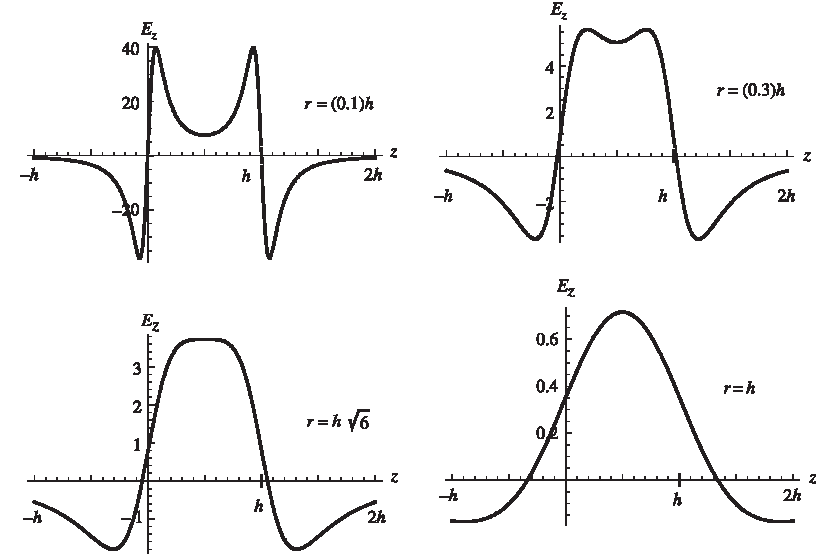
\includegraphics[width=\textwidth]{Anh/c2.pdf}
            \end{center}
        \end{enumerate}
       
    \end{loigiai}
    \begin{vd}[Điện tích xuyên vòng]
Cho hai vòng kim loại mảnh giống hệt nhau, bán kính $R$, mỗi vòng có điện tích $Q$ $(Q > 0)$ được phân bố đều trên toàn vòng. Hai vòng được đặt cố định song song với nhau trong chân không, khoảng cách giữa hai vòng là $2R$. Chọn trục tọa độ $\mathrm{O}x$ trùng với trục đối xứng của hai vòng với gốc tọa độ $\mathrm{O}$ đặt tại điểm cách đều hai vòng (xem hình vẽ). 
\begin{enumerate}[1)]
    \item Xác định cường độ điện trường tại điểm bất kì trên trục $x$.
    \item Một điện tích dương $q$, khối lượng $m$ chuyển động dọc theo trục $x$ từ xa vô cùng lại gần hai vòng với vận tốc ban đầu $v_0$. Bằng phương pháp đồ thị, hãy cho biết $v_0$ phải thỏa mãn điều kiện gì để điện tích $q$ có thể đi đến gốc tọa độ.
    \item Liệu có tồn tại vị trí mà ta có thể đặt điện tích $q$ nằm yên ở đó không? Nếu có thì đó là vị trí cân bằng bền hay không bền?
    \item Điện tích $q$ được giữ tại điểm trên trục $x$ có tọa độ $x_0 \ (0<x_0\ll R)$ Tại thời điểm $t=0$ thả nhẹ điện tích $q$ ra. Hãy xác định vị trí của $q$ ở thời điểm $t$ bất kì.
\end{enumerate}
\begin{center}


\tikzset{every picture/.style={line width=0.75pt}} %set default line width to 0.75pt        

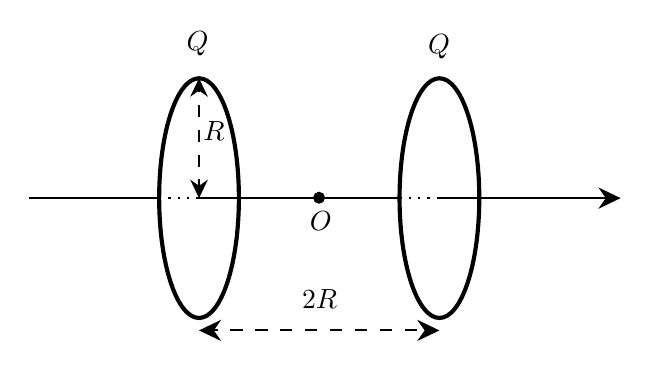
\begin{tikzpicture}[x=0.75pt,y=0.75pt,yscale=-1,xscale=1]
%uncomment if require: \path (0,300); %set diagram left start at 0, and has height of 300

%Straight Lines [id:da8992780354065661] 
\draw    (327.87,152.66) -- (369.78,152.66) -- (412.17,152.66) ;
\draw [shift={(415.17,152.66)}, rotate = 180] [fill={rgb, 255:red, 0; green, 0; blue, 0 }  ][line width=0.08]  [draw opacity=0] (10.72,-5.15) -- (0,0) -- (10.72,5.15) -- (7.12,0) -- cycle    ;
%Shape: Ellipse [id:dp5452127600171381] 
\draw  [line width=1.5]  (192.85,152.66) .. controls (192.85,120.77) and (201.45,94.92) .. (212.06,94.92) .. controls (222.67,94.92) and (231.26,120.77) .. (231.26,152.66) .. controls (231.26,184.55) and (222.67,210.4) .. (212.06,210.4) .. controls (201.45,210.4) and (192.85,184.55) .. (192.85,152.66) -- cycle ;
%Straight Lines [id:da748234131447068] 
\draw  [dash pattern={on 4.5pt off 4.5pt}]  (215.06,216.4) -- (324.87,216.4) ;
\draw [shift={(327.87,216.4)}, rotate = 180] [fill={rgb, 255:red, 0; green, 0; blue, 0 }  ][line width=0.08]  [draw opacity=0] (10.72,-5.15) -- (0,0) -- (10.72,5.15) -- (7.12,0) -- cycle    ;
\draw [shift={(212.06,216.4)}, rotate = 0] [fill={rgb, 255:red, 0; green, 0; blue, 0 }  ][line width=0.08]  [draw opacity=0] (10.72,-5.15) -- (0,0) -- (10.72,5.15) -- (7.12,0) -- cycle    ;
%Shape: Ellipse [id:dp7523961013690177] 
\draw  [line width=1.5]  (308.67,152.66) .. controls (308.67,120.77) and (317.27,94.92) .. (327.87,94.92) .. controls (338.48,94.92) and (347.08,120.77) .. (347.08,152.66) .. controls (347.08,184.55) and (338.48,210.4) .. (327.87,210.4) .. controls (317.27,210.4) and (308.67,184.55) .. (308.67,152.66) -- cycle ;
%Straight Lines [id:da19548217072294993] 
\draw    (212.06,152.66) -- (308.67,152.66) ;
%Straight Lines [id:da05665051754981065] 
\draw    (130,152.66) -- (192.85,152.66) ;
%Straight Lines [id:da1793421587844577] 
\draw  [dash pattern={on 0.84pt off 2.51pt}]  (192.85,152.66) -- (212.06,152.66) ;
%Straight Lines [id:da22689284080897432] 
\draw  [dash pattern={on 0.84pt off 2.51pt}]  (308.67,152.66) -- (327.87,152.66) ;
%Straight Lines [id:da20345355752484995] 
\draw  [dash pattern={on 4.5pt off 4.5pt}]  (212.06,149.66) -- (212.06,97.92) ;
\draw [shift={(212.06,94.92)}, rotate = 450] [fill={rgb, 255:red, 0; green, 0; blue, 0 }  ][line width=0.08]  [draw opacity=0] (8.93,-4.29) -- (0,0) -- (8.93,4.29) -- (5.93,0) -- cycle    ;
\draw [shift={(212.06,152.66)}, rotate = 270] [fill={rgb, 255:red, 0; green, 0; blue, 0 }  ][line width=0.08]  [draw opacity=0] (8.93,-4.29) -- (0,0) -- (8.93,4.29) -- (5.93,0) -- cycle    ;
%Shape: Circle [id:dp7863875363556825] 
\draw  [color={rgb, 255:red, 0; green, 0; blue, 0 }  ,draw opacity=1 ][fill={rgb, 255:red, 0; green, 0; blue, 0 }  ,fill opacity=1 ] (267.52,152.46) .. controls (267.52,151.16) and (268.58,150.11) .. (269.88,150.11) .. controls (271.18,150.11) and (272.24,151.16) .. (272.24,152.46) .. controls (272.24,153.77) and (271.18,154.82) .. (269.88,154.82) .. controls (268.58,154.82) and (267.52,153.77) .. (267.52,152.46) -- cycle ;


% Text Node
\draw (204.56,71.04) node [anchor=north west][inner sep=0.75pt]    {$Q$};
% Text Node
\draw (320.96,72.2) node [anchor=north west][inner sep=0.75pt]    {$Q$};
% Text Node
\draw (212.63,114.11) node [anchor=north west][inner sep=0.75pt]    {$R$};
% Text Node
\draw (263.92,157.86) node [anchor=north west][inner sep=0.75pt]    {$O$};
% Text Node
\draw (260.17,195.27) node [anchor=north west][inner sep=0.75pt]    {$2R$};


\end{tikzpicture}
\end{center}
\end{vd}
\begin{loigiai}
    \begin{enumerate}[1)]
        \item Ta xác định điện thế tại điểm M bất kì trên trục $x$. Chọn mốc tính điện thế là điểm xa vô cùng. Các phần tử trên mỗi vòng tròn đều các $M$ các khoảng bằng nhau nên điện thế tại $M$ là:
        \[V(x) = \dfrac{1}{4 \pi \varepsilon_0}\dfrac{Q}{\sqrt{R^2+\left(x-R\right)^2}}+\dfrac{1}{4 \pi \varepsilon_0} \dfrac{Q}{\sqrt{R^2+\left(x+R\right)^2}}. \tag{1} \label{tr.tst.2.1}\]
        Từ đó: \[E(x)=-\dfrac{\dd V(x)}{\dd x}=\dfrac{Q}{{4\pi {\varepsilon _0}}}\left\{ {\dfrac{{Q\left( {x - R} \right)}}{{{{\left[ {{R^2} + {{\left( {x - R} \right)}^2}} \right]}^{\frac{3}{2}}}}} + \dfrac{{Q\left( {x + R} \right)}}{{{{\left[ {{R^2} + {{\left( {x + R} \right)}^2}} \right]}^{\frac{3}{2}}}}}} \right\}. \tag{2}\]
        \item Khi đặt tại $M$ điện tích $q$, thế năng của hệ là:
        \[U( x ) = qV( x ) = \dfrac{1}{{4\pi {\varepsilon _0}}}\dfrac{{qQ}}{{\sqrt {{R^2} + {{\left( {x - R} \right)}^2}} }} + \dfrac{1}{{4\pi {\varepsilon _0}}}\dfrac{{qQ}}{{\sqrt {{R^2} + {{\left( {x + R} \right)}^2}} }}. \tag{3}\]
        Để xét sự biến thiên của $U(x)$, ta xét phương trình:
        \[\dfrac{\dd}{{\dd{{x}}}}U(x) =  - qE(x) =  - \dfrac{{qQ}}{{4\pi {\varepsilon _0}}}\left\{ {\dfrac{{x - R}}{{{{\left[ {{R^2} + {{\left( {x - R} \right)}^2}} \right]}^{\frac{3}{2}}}}} + \dfrac{{x + R}}{{{{\left[ {{R^2} + {{\left( {x + R} \right)}^2}} \right]}^{\frac{3}{2}}}}}} \right\} = 0. \tag{4} \label{tr.tst.2.4}\]
        \textit{Nhận xét}: Trong miền $|x|\geqslant R, \dfrac{\dd}{\dd x}U(x) \ne 0 $. Do đó, nghiệm của phương trình (\ref{tr.tst.2.4}) nằm trong khoảng $(-R,R)$, tức là các điểm cực trị của $U(x)$ nằm trong khoảng $(-R,R)$.
        Xét điện trường có cường độ $E^*$ gây bởi một vòng dây, gốc tọa độ đặt tại tâm của vành.
        Điện thế tại điểm có tọa độ $x$ là:
        \[V(x) = \dfrac{1}{{4\pi {\varepsilon _0}}}\dfrac{Q}{{\sqrt {{R^2} + {x^2}} }}\]
        \[ \Rightarrow {E^{*}}(x) =  - \dfrac{{dV(x)}}{{dx}} = \dfrac{1}{{4\pi {\varepsilon _0}}}\dfrac{{Qx}}{{\sqrt {{{\left( {{R^2} + {x^2}} \right)}^3}} }}.\]
        Do đó
        \[\dfrac{{dE^{*}(x)}}{{dx}} = \dfrac{1}{{4\pi {\varepsilon _0}}}\dfrac{{Q\left( {{R^2} - 2{x^2}} \right)}}{{{{\left( {{R^2} + {x^2}} \right)}^{\frac{5}{2}}}}}.\]
        \begin{center}
            

\tikzset{every picture/.style={line width=0.75pt}} %set default line width to 0.75pt        

\begin{tikzpicture}[x=0.75pt,y=0.75pt,yscale=-1,xscale=1]
%uncomment if require: \path (0,300); %set diagram left start at 0, and has height of 300

%Straight Lines [id:da29340981265573385] 
\draw    (109,127.34) -- (391.4,127.34) ;
%Straight Lines [id:da10824321089642597] 
\draw    (250.2,46.13) -- (250.2,208.54) ;
%Straight Lines [id:da28917983880229525] 
\draw  [dash pattern={on 4.5pt off 4.5pt}]  (202.88,127.72) -- (202.88,205.2) ;
%Curve Lines [id:da2132070532280097] 
\draw    (151.22,161.94) .. controls (200.94,184.54) and (195.13,263.31) .. (250.2,127.34) ;

%Straight Lines [id:da09829234828261857] 
\draw  [dash pattern={on 4.5pt off 4.5pt}]  (297.33,126.69) -- (297.33,104.48) -- (297.33,49.21) ;
%Curve Lines [id:da28912635664334707] 
\draw    (349.18,92.73) .. controls (299.46,70.13) and (305.27,-8.63) .. (250.2,127.34) ;


% Text Node
\draw (178.85,77.91) node [anchor=north west][inner sep=0.75pt]    {$-\dfrac{1}{\sqrt{2}}$};
% Text Node
\draw (282.63,131.69) node [anchor=north west][inner sep=0.75pt]    {$\dfrac{1}{\sqrt{2}}$};
% Text Node
\draw (230.7,46.6) node [anchor=north west][inner sep=0.75pt]    {$E^{*}$};
% Text Node
\draw (353.66,108.67) node [anchor=north west][inner sep=0.75pt]    {$x/R$};


\end{tikzpicture}
        \end{center}
        Vì $\dfrac{{\dd E^{*}(x)}}{{\dd x}} = \dfrac{1}{{4\pi {\varepsilon _0}}}\dfrac{{Q\left( {{R^2} - 2{x^2}} \right)}}{{{{\left( {{R^2} + {x^2}} \right)}^{\frac{5}{2}}}}}$, dễ dàng suy ra $E^{*}$ có giá trị cực đại $E^{*}_{\max}>0$ tại $\dfrac{R}{\sqrt{2}}$ và có giá trị cực tiểu âm $-E^{*}_{\max}$ tại $-\dfrac{R}{\sqrt{2}}$.
        
        Ngoài ra, $E^{*}>0$ với $x>0$ và $E^{*}<0$ với $x<0$.
        Kí hiệu $E_1$ và $E_2$ lần lượt là cường độ điện trường gây ra bởi vành đặt tại $x=R$ và vành đặt tại $x=-R$. Vì điện trường tổng hợp có tính chất $E(x)=-E(-x)$ nên ta chỉ cần xét miền $0 \leq x<R$.
        \\ Khi $x$ giảm dần từ $R$ đến $\left(1-\dfrac{1}{\sqrt{2}}\right)R$, $E_1$ giảm đơn điệu từ 0 đến giá trị $-E_{\max}$, còn $E_2$ luôn dương và tăng đơn điệu nhưng luôn nhỏ hơn $E_{\max}$. Do đó, điện trường tổng hợp $E$ có giá trị dương tại $x=R$ và có giá trị âm tại $\left(1-\dfrac{1}{\sqrt{2}}\right)R$. Vì $E$ là hàm liên tục của $x$ nên $E$ phải bằng 0 tại một điểm $x_1$ nào đó trong khoảng $\left( {\left( {1 - \dfrac{1}{{\sqrt 2 }}} \right)R,R} \right)$.
        \\ Khi $x$ giảm từ $\left(1-\dfrac{1}{\sqrt{2}}\right)R$ tới 0, $E_1$ tăng đơn điệu từ 0 đến giá trị $-E_0 (E_0>0)$ nào đó, còn $E_2$ luôn dương và tăng đơn điệu từ giá trị nhỏ hơn $E_{\max}$ đến giá trị $E_0$. Do đó, điện trường tổng hợp $E$ có giá trị âm trong khoảng $\left( {0,\left( {1 - \dfrac{1}{{\sqrt 2 }}} \right)R} \right)$. Đồ thị của $E$ được phác họa ở hình dưới.
        \begin{center}
            

\tikzset{every picture/.style={line width=0.75pt}} %set default line width to 0.75pt        

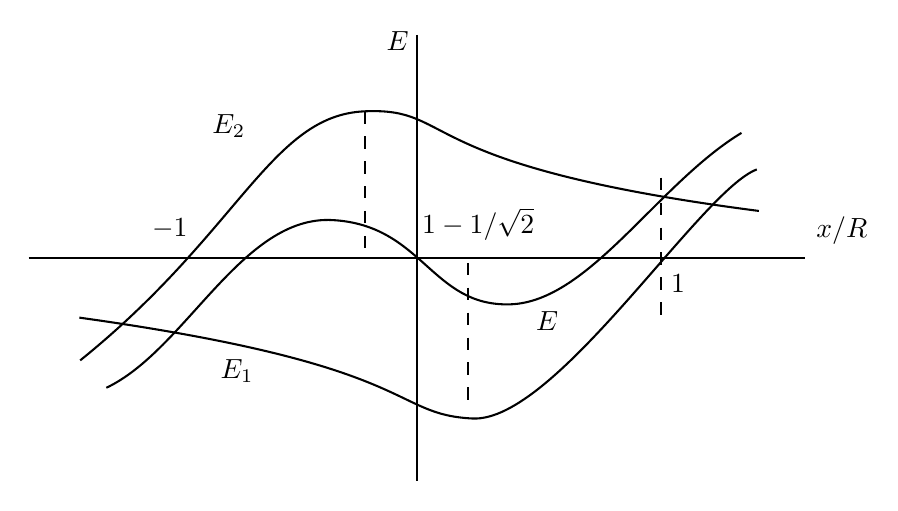
\begin{tikzpicture}[x=0.75pt,y=0.75pt,yscale=-1,xscale=1]
%uncomment if require: \path (0,300); %set diagram left start at 0, and has height of 300

%Straight Lines [id:da056701205338354876] 
\draw    (107,141.97) -- (481.09,141.97) ;
%Straight Lines [id:da34292327921721166] 
\draw    (294.05,34.4) -- (294.05,249.54) ;
%Curve Lines [id:da8479191662540728] 
\draw    (131.8,191.2) .. controls (208.8,129.2) and (223.8,73.2) .. (268.8,71.2) .. controls (313.8,69.2) and (288.8,97.2) .. (458.8,119.2) ;
%Curve Lines [id:da5196977908822733] 
\draw    (131.4,170.6) .. controls (296.4,193.6) and (280.8,217.2) .. (320.8,219.2) .. controls (360.8,221.2) and (430.8,109.2) .. (457.8,99.2) ;
%Curve Lines [id:da7681668515968598] 
\draw    (144.4,204.4) .. controls (182.8,186.2) and (209.8,121.2) .. (253.4,123.6) .. controls (297,126) and (300.8,165.2) .. (338.8,164.2) .. controls (376.8,163.2) and (409.8,106.2) .. (450.4,81.6) ;
%Straight Lines [id:da10982613158159515] 
\draw  [dash pattern={on 4.5pt off 4.5pt}]  (268.8,71.2) -- (268.8,142.2) ;
%Straight Lines [id:da5867849954172704] 
\draw  [dash pattern={on 4.5pt off 4.5pt}]  (318.8,144.2) -- (318.8,215.2) ;
%Straight Lines [id:da4065785269483002] 
\draw  [dash pattern={on 4.5pt off 4.5pt}]  (411.8,103.2) -- (411.8,174.2) ;


% Text Node
\draw (165,121.4) node [anchor=north west][inner sep=0.75pt]    {$-1$};
% Text Node
\draw (295,116.4) node [anchor=north west][inner sep=0.75pt]    {$1-1/\sqrt{2}$};
% Text Node
\draw (415,148.4) node [anchor=north west][inner sep=0.75pt]    {$1$};
% Text Node
\draw (198,189.4) node [anchor=north west][inner sep=0.75pt]    {$E_{1}$};
% Text Node
\draw (194,71.4) node [anchor=north west][inner sep=0.75pt]    {$E_{2}$};
% Text Node
\draw (350,166.4) node [anchor=north west][inner sep=0.75pt]    {$E$};
% Text Node
\draw (485,120.4) node [anchor=north west][inner sep=0.75pt]    {$x/R$};
% Text Node
\draw (278,31.4) node [anchor=north west][inner sep=0.75pt]    {$E$};


\end{tikzpicture}
        \end{center}
        Tóm lại, điện trường tổng hợp $E$ bằng không tại ba điểm $x=0$ và $x=\pm x_1$. Điều đó có nghĩa là $\dfrac{\dd U}{\dd x}=0$ tại các điểm nói trên.
        \\Vậy $U(x)$ đạt cực tiểu tại $x=0$ và đạt cực đại tại $x=\pm x_1$. Kí hiệu $U_{\max}=U(x_1)$. Ta thấy để hạt $q$ có thể đi tới gốc tọa độ $x=0$ thì động năng ban đầu của nó phải lớn hơn $U_{\max}$, tức vận tốc ban đầu của nó phải thỏa mãn điều kiện: \[v_0>\dfrac{2U_{\max}}{m}.\]
        \item Như trên, ta thấy tồn tại ba vị trí cân bằng $x=0$ và $x=\pm x_1$, trong đó $x=0$ là vị trí cân bằng bền, còn hai vị trí còn lại là không bền.
        \item Tại lân cận điểm 0, tức là với $|x|\ll R$, ta có
        \[\dfrac{{\dd U(x)}}{{\dd x}} =  - \dfrac{{qQ}}{{4\pi {\varepsilon _0}}}\left\{ {\dfrac{{x - R}}{{{{\left[ {{R^2} + {{\left( {x - R} \right)}^2}} \right]}^{\frac{3}{2}}}}} + \dfrac{{x + R}}{{{{\left[ {{R^2} + {{\left( {x + R} \right)}^2}} \right]}^{\frac{3}{2}}}}}} \right\}.\]
        Khai triển mẫu số, bỏ qua $x^2$ so với $x$ ta được
        \[\dfrac{{\dd U(x)}}{{\dd x}} \approx \dfrac{{qQ}}{{4\pi {\varepsilon _0}}}\left\{ {\dfrac{{x - R}}{{{{\left[ {2{{R}}\left( {R - x} \right)} \right]}^{\frac{3}{2}}}}} + \dfrac{{x + R}}{{{{\left[ {2{{R}}\left( {R - x} \right)} \right]}^{\frac{3}{2}}}}}} \right\}.\]
        \[ \Rightarrow \dfrac{{\dd U(x)}}{{\dd x}} = \dfrac{{qQ}}{{8\sqrt 2 \pi {\varepsilon _0}{R^3}}}x. \tag{5} \label{tr.tst.2.5}\]
        Theo (\ref{tr.tst.2.5}), phương trình chuyển động của $q$ là $m\Ddot{x}=-kx$ với $|x|\ll R$, trong đó $k=\dfrac{{qQ}}{{8\sqrt 2 \pi {\varepsilon _0}{R^3}}}$.
        \\Điều này có nghĩa là $q$ dao động điều hòa xung quanh gốc tọa độ. Vị trí của $q$ tại thời điểm $t>0$ bất kì là $x=x_0 \cos{(\omega t)}$ với $\omega  = \dfrac{1}{2}\sqrt {\dfrac{{qQ}}{{\sqrt 2 \pi {\varepsilon _0}m{{{R}}^3}}}}$.
     \end{enumerate}
\end{loigiai}

 \begin{vd}[``Nhiều'' năng lượng]
    \label{c291}
    Một điện tích $Q$ được phân bố đều trong một quả cầu bán kính $R$. Tìm năng lượng tĩnh điện của phân bố điện tích này theo ba cách sau 
    \begin{enumerate}[1)]
    \setlength{\itemsep}{0pt}
        \item Tính công cần để thiết lập phân bố điện tích bằng cách di chuyển các vỏ cầu nhỏ tích điện từ vô cùng đến vị trí cuối cùng của chúng.
        \item Tính năng lượng điện trường bằng cách tích phân mật độ năng lượng điện trường $u_e=\dfrac{E^2}{8\pi \varepsilon_0}$ theo thể tích.
        \item Tính thế năng tĩnh điện của hệ bằng cách tính tích phân $\dfrac{\rho\phi}{2}$ theo thể tích, với $\rho$ là mật độ điện tích, $\phi$ là điện thế. Cách tính này khác gì với phép tính trong ý trước?
    \end{enumerate}
    \end{vd}
    \begin{loigiai}
    \begin{enumerate}[1)]
    \setlength{\itemsep}{0pt}
        \item Ta có thể xây dựng quả cầu này bằng cách di chuyển những vỏ cầu nhỏ từ vô cùng đến vị trí cuối cùng của chúng.  Giả sử tại một thời điểm nào đó, chúng ta đã có một quả cầu tích điện $\rho$ và bán kính $r<R$.\\
        Điện tích của quả cầu:
        $$q(r)=\dfrac{4\pi r^3\rho}{3}.$$
        Điện thế tại bề mặt quả cầu:
        \begin{equation*}
            \begin{aligned}
                \phi(r)=\dfrac{kq(r)}{r}
                =\dfrac{r^2\rho}{3\varepsilon_0}.
            \end{aligned}
        \end{equation*}
        Bây giờ ta sẽ di chuyển các điện tích từ vô cùng đến vị trí cuối cùng của nó để ``bồi'' thêm cho quả cầu một lớp cầu dày $\dd r$.\\
        Điện tích một lớp cầu:
        \begin{equation*}
            \dd q=4\pi r^2\dd r\rho.
        \end{equation*}
        Công để dịch chuyển lớp cầu này:
        \begin{equation*}
            \begin{aligned}
                \dd W&=\phi(r)\dd q\\
                &=\dfrac{r^2\rho}{3\varepsilon_0}\tron{4\pi r^2\dd r\rho}\\
               &=\dfrac{4\pi\rho^2 r^4 \dd r}{3\varepsilon_0}.
            \end{aligned}
        \end{equation*}
        Công tổng cộng cần để tạo ra một quả cầu bán kính $R$:
        \begin{equation*}
            \begin{aligned}
                W&=\tiph{0}{R}{\dfrac{4\pi\rho^2 r^4}{3\varepsilon_0}}{r}\\
                &=\dfrac{4\pi\rho^2}{3\varepsilon_0}\left.\tron{\dfrac{r^5}{5}}\right|_0^R\\
                &=\dfrac{4\pi\rho^2 R^5}{15\varepsilon_0}=\dfrac{3kQ^2}{5R}.\\
            \end{aligned}
        \end{equation*}
        Với $Q=\dfrac{4\pi R^3\rho}{3}$ là điện tích của quả cầu.
        \item Ta xét điện trường tạo ra bởi phân bố điện tích trên tại một điểm cách tâm hình cầu một khoảng $r$.\\
        Với $r>R$, điện trường giống như là điện trường của một điện tích điểm $Q$ đặt tại tâm hình cầu:
        \begin{equation*}
            E=\dfrac{kQ}{r^2}.
        \end{equation*}
        Với $r\leq R$, ta sử dụng định luật Gauss.\\
        Chọn mặt Gauss là một mặt cầu có bán kính $r$, tâm trùng với tâm quả cầu. Ta có:
        \begin{equation*}
            \begin{aligned}
                E\tron{4\pi r^2}=\dfrac{r^3Q}{R^3\varepsilon_0}
                \Leftrightarrow E=\dfrac{kQr}{R^3}.
            \end{aligned}
        \end{equation*}
        Tích phân mật độ năng lượng điện trường trên toàn bộ thể tích:
        \begin{equation*}
            \begin{aligned}
                W&=\tiph{0}{\infty}{\dfrac{E^2(r)}{8\pi k}4\pi r^2}{r}\\
                &=\dfrac{kQ^2}{2}\tron{\tiph{0}{R}{\tron{\dfrac{r}{R^3}}^2r^2}{r}+\tiph{R}{\infty}{\tron{\dfrac{1}{r^2}}^2r^2}{r}}\\
                &=\dfrac{kQ^2}{2}\tron{\dfrac{1}{5R}+\dfrac{1}{R}}=\dfrac{3kQ^2}{5R}.
            \end{aligned}
        \end{equation*}
        \item Điện thế trên bề mặt quả cầu: 
        $$\phi_0=\dfrac{kQ}{R}.$$
        Với $r<R$, ta có:
        \begin{equation*}
        \begin{aligned}
             &\ ~~~ \dd \phi &=& -E\dd r\\
             \Leftrightarrow ~& \phi_0-\phi(r) &=&-\tiph{r}{R}{\dfrac{kQr'}{R^3}}{r'}\\
             \Leftrightarrow~ &\quad \phi(r)&=&\dfrac{kQ}{R}+\dfrac{kQ\tron{R^2-r^2}}{2R^3}\\
             &\ &=&\dfrac{3kQ}{2R}-\dfrac{kQr^2}{2R^3}.
        \end{aligned}
        \end{equation*}
        Thế năng tĩnh điện của hệ: 
        \begin{equation*}
            \begin{aligned}
                W&=\tiph{0}{R}{\dfrac{1}{2}\phi(r)\rho 4\pi r^2}{r}\\
                &=\tiph{0}{R}{\tron{\dfrac{3kQ}{2R}-\dfrac{kQr^2}{2R^3}}\tron{\dfrac{3Qr^2}{R^3}}}{r}\\
                &=\dfrac{kQ^2}{4}\left.\tron{\dfrac{3r^3}{R^4}-\dfrac{3r^5}{5R^6}}\right|_0^R\\
                &=\dfrac{3kQ^2}{5R}.
            \end{aligned}
        \end{equation*}
    \end{enumerate}
    Ta thấy được từ ba phần trên, cả ba phương pháp đều đi đến cùng một kết quả. Tuy nhiên, so sánh giữa phương pháp ở phần thứ hai và phần thứ ba, ta thấy rằng khái niệm mật độ năng lượng điện trường không đơn thuần có nghĩa là ``năng lượng chứa trong một đơn vị thể tích''. Nếu chúng ta coi mật độ năng lượng là $u_e=\dfrac{E^2}{8\pi \varepsilon_0}$, thì điều đó có nghĩa là năng lượng sẽ trải rộng trên toàn bộ không gian. Còn nếu ta coi mật độ năng lượng là $\dfrac{\rho\phi}{2}$, điều này có nghĩa là năng lượng chỉ tập trung tại nơi có mặt điện tích. Vậy nên, khái niệm mật độ năng lượng là một khái niệm khá là trừu tượng, trong khi năng lượng của một hệ lại là một đại lượng được định nghĩa chính xác, ít nhất là trong trường hợp không xuất hiện điện tích điểm.
    \end{loigiai}
    
    
    \begin{vd}[Lỗ trên mặt phẳng]
    \begin{enumerate}[1)]
    \setlength{\itemsep}{0pt}
        \item Người ta cắt một lỗ tròn bán kính $R$ trên một tấm phẳng rộng tích diện đều với mật độ điện tích mặt $\sigma$. Đường thẳng $\Delta$ vuông góc với mặt phẳng và đi qua tâm của lỗ. Tìm điện trường tại một điểm trên $\Delta$, cách tâm lỗ một khoảng là $z$.
        \item Một điện tích điểm $-q$, khối lượng $m$ được thả từ một vị trí trên $\Delta$, rất gần tâm của lỗ. Chứng minh rằng điện tích dao động điều hòa và tìm tần số góc $\omega$ của dao động.\\
        Tính $\omega$ với $m=1\dv{g}$, $-q=-10^{-8}\dv{C}$, $\sigma=10^{-6}\dv{C/m^2}$ và $R=0,1\dv{m}$.
        \item Một điện tích $-q$ khối lượng $m$ được thả từ một vị trí trên trục $\Delta$ và cách tấm một khoảng là $z$. Tìm vận tốc điện tích điểm khi nó đi qua tâm lỗ. Đánh giá kết quả của bạn khi $z\gg R$.
    \end{enumerate}
    \end{vd}
    \begin{loigiai}
        \begin{enumerate}[1)]
        \setlength{\itemsep}{0pt}
            \item Xét một phần tử diện tích có điện tích $\dd q$ cách tâm của lỗ tròn là $r$. Điện trường do phần tử này gây ra tại điểm đang xét là $\dfrac{\dd q}{4\pi \varepsilon_0\tron{r^2+z^2}}$. Do tính chất đối xứng của hệ, điện trường tại một điểm trên đường thẳng $\Delta$ có phương dọc theo $\Delta$, vậy nên chỉ có thành phần điện trường dọc theo $\Delta$ mới đóng góp vào điện trường tổng hợp. Ta có:
            \begin{equation}
                \dd E=\dfrac{\dd q}{4\pi \varepsilon_0\tron{r^2+z^2}}\frac{z}{\sqrt{r^2+z^2}}.
                \label{ca4}
            \end{equation}
            Ta có $\dd q=\sigma r\dd r\dd \theta$. \\
            \newpage
            Điện trường do toàn bộ mặt phẳng (có lỗ) sinh ra:
            \begin{equation}
               \begin{aligned}
                  E(z)&=\int_R^\infty\int_0^{2\pi}\dfrac{\sigma zr}{4\pi \varepsilon_0\tron{r^2+z^2}^\frac{3}{2}}\dd r \dd \theta\\
                  &=\int_R^\infty\dfrac{2\pi \sigma zr}{4\pi \varepsilon_0\tron{r^2+z^2}^\frac{3}{2}}\dd r \\
                  &=\left.-\dfrac{2\pi \sigma z}{4\pi \varepsilon_0\sqrt{r^2+z^2}}\right|_R^\infty\\
                  &=\dfrac{\sigma z}{2\varepsilon_0\sqrt{R^2+z^2}}.
                  \label{ca4}
               \end{aligned} 
            \end{equation}
            Chú ý rằng khi $R=0$, điện trường sẽ là $E=\dfrac{\sigma}{2\varepsilon_0}$ giống điện trường của một mặt phẳng vô hạn tích điện đều.
            \item Khi $z\ll R$, thì từ (\ref{ca4}) ta có $E(z)\approx \dfrac{\sigma z}{2\varepsilon_0R}$. Phương trình chuyển động của điện tích  là:
            \begin{equation}
                -qE=m\ddot z\Leftrightarrow \ddot z+\tron{\dfrac{q\sigma}{2\varepsilon_0mR}}z=0.
            \end{equation}
            Điện tích dao động điều hòa. Tần số góc của dao động là:
            \begin{equation}
                \omega=\sqrt{\dfrac{q\sigma}{2\varepsilon_0mR}}.
            \end{equation}
            Thay số vào ta được:
            \begin{equation}
                \omega=\sqrt{\dfrac{\tron{10^{-8}\dv{C}}\tron{10^{-6}\dv{C/m^2}}}{2\tron{8,85\cdot10^{-12}\dv{\frac{s^2C^2}{kg\ m^3}}}\tron{10^{-3}\dv{kg}}\tron{0,1\dv{m}}}}=2,4\dv{s^{-1}}.
            \end{equation}
            Tần số góc này tương đương với tần số khoảng $0,4\dv{Hz}$. Để có dao động điểu hòa thì chuyển động của điện tích phải bị giới hạn trên đường thẳng $\Delta$ vì cân bằng của điện tích theo phương song song với mặt phẳng là cân bằng không bền.
            \item Thế năng của điện tích là $U(z)$. Ta có:
            \begin{equation}
            \begin{aligned}
                 &\dd U&=&-F\dd z=qE(z)\dd z\\
                 \Rightarrow &U(z)&=&\tiph{0}{z}{qE(z')}{z'}=\tiph{0}{z}{\dfrac{q\sigma z'}{2\varepsilon_0\tron{R^2+z'^2}}}{z'}\\
                 & \ &=&\left.\dfrac{q\sigma}{2\varepsilon_0}\sqrt{R^2+z'^2}\right|_0^z=\dfrac{q\sigma}{2\varepsilon_0}\tron{\sqrt{R^2+z^2}-R}.
            \end{aligned}
            \end{equation}
            Bảo toàn năng lượng, ta có:
            \begin{equation}
                \begin{aligned}
                   &\dfrac{mv^2}{2}=U(z)\\ \Leftrightarrow&v=\sqrt{\dfrac{q\sigma}{m\varepsilon_0}\tron{\sqrt{R^2+z^2}-R}}.
                \end{aligned}
            \end{equation}
            Với $z\gg R$, ta có $v\approx\sqrt{\dfrac{q\sigma z}{m\varepsilon_0}}$. Kết quả này giống như việc coi mặt phẳng là không có lỗ. Thật vậy, khi đó lực điện tác dụng lên điện tích sẽ là $\dfrac{q\sigma}{2\varepsilon_0}$ không đổi, gia tốc điện tích là $a=\dfrac{q\sigma}{2m\varepsilon_0}$. Vận tốc của điện tích khi chạm mặt phẳng là $v=\sqrt{2az}=\sqrt{\dfrac{q\sigma z}{m\varepsilon_0}}$.
        \end{enumerate}
    \end{loigiai}
    
    
    \begin{vd}[Kiểm chứng lại định luật Coulomb]
    Cavendish và Maxwell đã thực hiện các thí nghiệm để kiểm chứng lại tính đúng đắn của định luật Coulomb, rằng lực điện giữa hai điện tích điểm tỉ lệ nghịch với bình phương khoảng cách giữa chúng. Trong bài toán này chúng ta sẽ tìm hiểu về phần lý thuyết đằng sau những thí nghiệm này.
    \begin{enumerate}[1)]
    \setlength{\itemsep}{0pt}
        \item Giả sử rằng định luật Coulomb cho rằng lực điện giữa hai điện tích có dạng $\dfrac{kq_1q_2}{r^{2+\delta}}$. Cho một hệ gồm một vỏ cầu rỗng bán kính $R$ tích điện đều với điện tích $Q$, chứng tỏ rằng điện thế tại một điểm cách tâm vỏ cầu một khoảng là $r$ tuân theo quy luật sau:
        \begin{equation}
            \begin{aligned}
               &\phi(r)=\dfrac{kQ}{2\tron{1-\delta^2}rR}\tron{f(R+r)-f(R-r)}\qquad \text{(với $r<R$)},\\
               &\phi(r)=\dfrac{kQ}{2\tron{1-\delta^2}rR}\tron{f(R+r)-f(r-R)}\qquad \text{(với $r>R$)}.
            \end{aligned}
            \label{ca6}
        \end{equation}
        Trong đó $f(x)=x^{1-\delta}$ và $k=\dfrac{1}{4\pi\varepsilon_0}$.\\
        \textit{Lưu ý: Trong thực tế chúng ta quan tâm tới trường hợp $\delta\ll1$, vì vậy chúng ta có thể bỏ quả hạng tử $(1-\delta^2)$ ở mẫu số trong biểu thức (\ref{ca6}) và coi nó xấp xỉ 1. Chúng ta sẽ bỏ qua hạng tử này trong phần còn lại của bài toán.}
        \item Xét hai vỏ cầu đồng tâm với bán kính $a$ và $b$ (với $a>b$) và có điện tích lần lượt là $Q_a$ và $Q_b$ phân bố đều trên bề mặt. Chứng tỏ rằng điện thế ở trên từng mặt cầu được cho bởi công thức:
        \begin{equation}
            \begin{aligned}
                &\phi_a=\dfrac{kQ_a}{2a^2}f(2a)+\dfrac{kQ_b}{2ab}\tron{f(a+b)-f(a-b)},\\
                &\phi_b=\dfrac{kQ_b}{2b^2}f(2b)+\dfrac{kQ_a}{2ab}\tron{f(a+b)-f(a-b)}.
            \end{aligned}
        \end{equation}
        \item Nếu hai quả cầu được nối với nhau bằng dây mảnh dẫn điện, và được tích điện đến cùng điện thế $\phi$. Chứng tỏ rằng điện thế trên vỏ cầu bên trong (có bán kính $b$) lúc này là:
        \begin{equation}
            \begin{aligned}
                Q_b=\dfrac{2b\phi}{k}\dfrac{bf(2a)-a\tron{f(a+b)-f(a-b)}}{f(2a)+f(2b)-\tron{f(a+b)-f(a-b)}^2}.
            \end{aligned}
        \end{equation}
        Nếu $\delta=0$ thì $f(x)=x$, thì $Q_b=0$, giống như mong đợi. Nếu như $Q_b$ khác không thì $\delta$ cũng phải khác không.\\
        Với giá trị $\delta$ nhỏ thì bạn có thể sử dụng những phép tính gần đúng hợp lí để làm bài tập này.
    \end{enumerate}
    \end{vd}
     \begin{loigiai}
    \begin{enumerate}[1)]
    \setlength{\itemsep}{0pt}
        \item Giống như với bài \ref{ca5}, để tính điện thế tại điểm $P$, chúng ta sẽ chia vỏ cầu thành nhiều vòng nhỏ. Khoảng cách từ điểm $P$ tới một điểm trên vòng sẽ là $l=\sqrt{R^2+r^2-2Rr\cos\theta}$. Diện tích của vòng nhỏ sẽ là $2\pi R^2 \sin\theta\dd\theta$, điện tích của vòng sẽ là $\dd Q=\sigma2\pi R^2 \sin\theta\dd\theta=\dfrac{Q\sin\theta\dd\theta}{2}$. 
        \newpage
        \begin{center}
            

\tikzset{every picture/.style={line width=0.75pt}} %set default line width to 0.75pt        

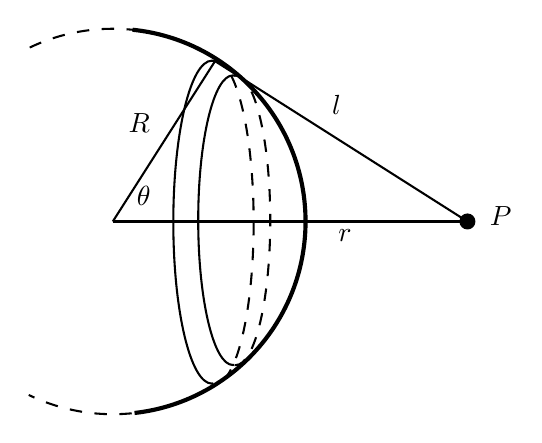
\begin{tikzpicture}[x=0.75pt,y=0.75pt,yscale=-1,xscale=1]
%uncomment if require: \path (0,300); %set diagram left start at 0, and has height of 300

%Shape: Arc [id:dp6604130734699976] 
\draw  [draw opacity=0][line width=1.5]  (338.38,47.48) .. controls (385.19,52.25) and (421.71,91.79) .. (421.71,139.85) .. controls (421.71,187.6) and (385.67,226.93) .. (339.32,232.12) -- (328.85,139.85) -- cycle ; \draw  [line width=1.5]  (338.38,47.48) .. controls (385.19,52.25) and (421.71,91.79) .. (421.71,139.85) .. controls (421.71,187.6) and (385.67,226.93) .. (339.32,232.12) ;
%Shape: Arc [id:dp3988355543248949] 
\draw  [draw opacity=0][dash pattern={on 4.5pt off 4.5pt}] (288.83,56.05) .. controls (300.95,50.25) and (314.52,47) .. (328.85,47) .. controls (380.14,47) and (421.71,88.57) .. (421.71,139.85) .. controls (421.71,191.14) and (380.14,232.71) .. (328.85,232.71) .. controls (314.33,232.71) and (300.59,229.37) .. (288.34,223.43) -- (328.85,139.85) -- cycle ; \draw  [dash pattern={on 4.5pt off 4.5pt}] (288.83,56.05) .. controls (300.95,50.25) and (314.52,47) .. (328.85,47) .. controls (380.14,47) and (421.71,88.57) .. (421.71,139.85) .. controls (421.71,191.14) and (380.14,232.71) .. (328.85,232.71) .. controls (314.33,232.71) and (300.59,229.37) .. (288.34,223.43) ;
%Shape: Arc [id:dp3770531364912999] 
\draw  [draw opacity=0] (377.32,217.94) .. controls (377.09,217.98) and (376.86,217.99) .. (376.63,217.99) .. controls (366.34,217.99) and (358,183.16) .. (358,140.18) .. controls (358,97.21) and (366.34,62.37) .. (376.63,62.37) .. controls (377.13,62.37) and (377.62,62.45) .. (378.11,62.61) -- (376.63,140.18) -- cycle ; \draw   (377.32,217.94) .. controls (377.09,217.98) and (376.86,217.99) .. (376.63,217.99) .. controls (366.34,217.99) and (358,183.16) .. (358,140.18) .. controls (358,97.21) and (366.34,62.37) .. (376.63,62.37) .. controls (377.13,62.37) and (377.62,62.45) .. (378.11,62.61) ;
%Shape: Arc [id:dp48119814484050627] 
\draw  [draw opacity=0][dash pattern={on 4.5pt off 4.5pt}] (377.38,62.51) .. controls (377.61,62.47) and (377.84,62.46) .. (378.08,62.46) .. controls (388.37,62.46) and (396.71,97.29) .. (396.71,140.27) .. controls (396.71,183.24) and (388.37,218.08) .. (378.08,218.08) .. controls (377.58,218.08) and (377.09,218) .. (376.6,217.84) -- (378.08,140.27) -- cycle ; \draw  [dash pattern={on 4.5pt off 4.5pt}] (377.38,62.51) .. controls (377.61,62.47) and (377.84,62.46) .. (378.08,62.46) .. controls (388.37,62.46) and (396.71,97.29) .. (396.71,140.27) .. controls (396.71,183.24) and (388.37,218.08) .. (378.08,218.08) .. controls (377.58,218.08) and (377.09,218) .. (376.6,217.84) ;

%Shape: Arc [id:dp38971002723714365] 
\draw  [draw opacity=0] (387.33,208.95) .. controls (387.12,208.99) and (386.91,209) .. (386.71,209) .. controls (377.48,209) and (370,177.77) .. (370,139.23) .. controls (370,100.7) and (377.48,69.46) .. (386.71,69.46) .. controls (387.15,69.46) and (387.59,69.54) .. (388.03,69.68) -- (386.71,139.23) -- cycle ; \draw   (387.33,208.95) .. controls (387.12,208.99) and (386.91,209) .. (386.71,209) .. controls (377.48,209) and (370,177.77) .. (370,139.23) .. controls (370,100.7) and (377.48,69.46) .. (386.71,69.46) .. controls (387.15,69.46) and (387.59,69.54) .. (388.03,69.68) ;
%Shape: Arc [id:dp7448302847473949] 
\draw  [draw opacity=0][dash pattern={on 4.5pt off 4.5pt}] (387.38,69.59) .. controls (387.59,69.55) and (387.79,69.54) .. (388,69.54) .. controls (397.23,69.54) and (404.71,100.78) .. (404.71,139.31) .. controls (404.71,177.84) and (397.23,209.08) .. (388,209.08) .. controls (387.56,209.08) and (387.11,209) .. (386.68,208.86) -- (388,139.31) -- cycle ; \draw  [dash pattern={on 4.5pt off 4.5pt}] (387.38,69.59) .. controls (387.59,69.55) and (387.79,69.54) .. (388,69.54) .. controls (397.23,69.54) and (404.71,100.78) .. (404.71,139.31) .. controls (404.71,177.84) and (397.23,209.08) .. (388,209.08) .. controls (387.56,209.08) and (387.11,209) .. (386.68,208.86) ;

%Straight Lines [id:da6172667981511248] 
\draw    (328.85,139.85) -- (499.71,139.85) ;
\draw [shift={(499.71,139.85)}, rotate = 0] [color={rgb, 255:red, 0; green, 0; blue, 0 }  ][fill={rgb, 255:red, 0; green, 0; blue, 0 }  ][line width=0.75]      (0, 0) circle [x radius= 3.35, y radius= 3.35]   ;
%Straight Lines [id:da567536953964995] 
\draw    (378.11,62.61) -- (328.85,139.85) ;
%Straight Lines [id:da6026285341166078] 
\draw    (378.11,62.61) -- (499.71,139.85) ;

% Text Node
\draw (339,121.4) node [anchor=north west][inner sep=0.75pt]    {$\theta $};
% Text Node
\draw (335,86.4) node [anchor=north west][inner sep=0.75pt]    {$R$};
% Text Node
\draw (436,142.4) node [anchor=north west][inner sep=0.75pt]    {$r$};
% Text Node
\draw (433,77.4) node [anchor=north west][inner sep=0.75pt]    {$l$};
% Text Node
\draw (509,131.4) node [anchor=north west][inner sep=0.75pt]    {$P$};


\end{tikzpicture}

        \end{center}
        Nếu như lực điện giữa hai điện tích điểm có dạng như $F(r)=\dfrac{kq_1q_2}{r^{2+\delta}}$, thì điện thế gây ra bởi một điện tích điểm $\dd q$ tại một điểm cách điện tích một khoảng $l$ sẽ là $\dfrac{k\dd q}{\tron{1+\delta}l^{1+\delta}}$. Điện thế do vòng gây ra tại $P$ sẽ là:

            \[\dd\phi=\dfrac{kQ\sin\theta\dd\theta}{2(1+\delta)l^{1+\delta}}=\dfrac{kQ\sin\theta\dd\theta}{2(1+\delta)\tron{R^2+r^2-2Rr\cos\theta}^{\frac{1+\delta}{2}}}. \tag{1}\]

        Điện thế do cả vỏ cầu gây ra tại $P$ là:
        \[\begin{aligned}
           \phi(r)&=\tiph{0}{\pi}{\dfrac{kQ\sin\theta}{2(1+\delta)\tron{R^2+r^2-2Rr\cos\theta}^{\frac{1+\delta}{2}}}}{\theta}\\
           &=\left.\dfrac{kQ}{2\tron{1-\delta^2}rR}\tron{R^2+r^2-2Rr\cos\theta}^{\frac{1-\delta}{2}}\right|_0^\theta.
        \end{aligned} \tag{2}\]
        Bây giờ ta sẽ xét hai trường hợp. Nếu $r<R$, ta có:
           \[ \phi(r)=\dfrac{kQ}{2\tron{1-\delta^2}rR}\tron{f(R+r)-f(R-r)}.\tag{3}\]
        Nếu $r>R$, ta có:
        \[\phi(r)=\dfrac{kQ}{2\tron{1-\delta^2}rR}\tron{f(R+r)-f(r-R)}. \tag{4}\]
        Nếu như $\delta=0$ thì $f(x)=x$, kết quả thu được sẽ là $\dfrac{kQ}{R}$ với $r<R$ và $\dfrac{kQ}{r}$ với $r>R$, giống với kết quả trong bài \ref{ca5}.
        \item Điện thế do vỏ cầu lớn bán kính $a$ gây ra tại một điểm trên bề mặt nó là $\dfrac{kQ_a}{2a^2}f(2a)$, tại đây chúng ta đã bỏ qua hạng tử $\tron{1-\delta^2}$. Điện thế do vỏ cầu bé bán kính $b$ gây ra tại một điểm trên bề mặt vỏ cầu lớn là $\dfrac{kQ_b}{2ab}\tron{f(a+b)-f(a-b)}$. Điện thế tại một điểm trên bề mặt vỏ cầu lớn sẽ là tổng của hai điện thế trên:
            \[\phi_a=\dfrac{kQ_a}{2a^2}f(2a)+\dfrac{kQ_b}{2ab}\tron{f(a+b)-f(a-b)}. \tag{5}\label{cb3}\]
        Tương tự, điện thế do vỏ cầu nhỏ gây ra trên bề mặt nó là $\dfrac{kQ_b}{2b^2}f(2b)$, điện thế do vỏ cầu lớn gây ra trên bề mặt vỏ cầu nhỏ là $\dfrac{kQ_a}{2ab}\tron{f(a+b)-f(a-b)}$. Điện thế trên bề mặt vỏ cầu nhỏ:
            \[\phi_b=\dfrac{kQ_b}{2b^2}f(2b)+\dfrac{kQ_a}{2ab}\tron{f(a+b)-f(a-b)}.\tag{6}\label{cb4}
            \]
        Nếu $\delta=0$, $f(x)=x$ thì kết quả trên trở thành:
            \[\phi_a=\dfrac{kQ_a}{a}+\dfrac{kQ_b}{a}\quad \text{và} \quad \phi_b=\dfrac{kQ_a}{a}+\dfrac{kQ_b}{b}.
           \tag{7} \]
        Kết quả trên giống với khi ta sử dụng định luật Coulomb bình thường.
        \item Khi hai quả cầu được nối với nhau bằng dây dẫn và được tích điện tới cùng điện thế $\phi$, ta có $\phi_a=\phi_b=\phi$. Thay vào phương trình (\ref{cb3}) và (\ref{cb4}) và coi $Q_a$ và $Q_b$ là ẩn ta thu được một hệ hai phương trình hai ẩn. Nhân hai vế phương trình (\ref{cb3}) với $a\tron{f(a+b)-f(a-b)}$, phương trình (\ref{cb4}) với $bf(2a)$ rồi trừ vế với vế, ta được:
        \[\begin{aligned}
             \phi\Big(bf&(2a)-a\big[f(a+b)-f(a-b)\big]\Big)\\
             &=\dfrac{kQ_b}{2b}\Big(f(2a)f(2b)-\big[f(a+b)-f(a-b)\big]^2\Big). 
             \end{aligned}\tag{8} \]
        Từ đó, ta thu được:
            \[Q_b=\dfrac{2b\phi}{k}\dfrac{bf(2a)-a\big[f(a+b)-f(a-b)\big]}{f(2a)f(2b)-\big[f(a+b)-f(a-b)\big]^2}.\tag{9} \]
        Trong quá trình tính toán, ta đã bỏ qua hạng tử $(1-\delta^2)$, nếu ta không bỏ qua hạng tử này, thì nó sẽ xuất hiện ở tử số trong biểu thức tính $Q_b$. Giống như đã nêu ở đề bài, khi $\delta=0$ thì biểu thức của chúng ta cho kết quả $Q_b$ bằng không. Với giá trị $\delta$ nhỏ, ta có thể thực hiện phép tính gần đúng đến bậc nhất của $\delta$ để ước tính giá trị của $Q_b$. Nếu ta thay $a=1$ và $b=0,5$ thì $Q_b\approx\dfrac{2b\phi}{k}\tron{0,26\delta}$. Với $\delta$ nhỏ, điện tích trên vỏ cầu ngoài sẽ giống như là khi ta tính toàn với định luật Coulomb bình thường $Q_a=\dfrac{a\phi}{k}$. Vậy đối với $a=1$ và $b=0,5$ thì tỉ lệ điện tích trên hai vỏ cầu sẽ là:
        \begin{equation}
            \dfrac{Q_b}{Q_a}=\dfrac{\dfrac{2b\phi}{k}\tron{0,26\delta}}{\dfrac{a\phi}{k}}=0,26\delta.
        \end{equation}
    \end{enumerate}
    \end{loigiai}    
    
    
    \begin{vd}[Quả cầu bị cắt]
Một quả cầu kim loại bán kính $R$, được cắt thành hai nửa bởi một mặt phẳng sao cho diện tích chỏm cầu phần nhỏ hơn là $\pi.R^2$. Các mặt tiếp xúc được phủ một lớp cách điện rất mỏng, rồi ghép hai nửa lại với nhau để tạo thành quả cầu như ban đầu. Ban đầu tổng điện tích của quả cầu bằng $0$. Sau khi ghép, phần nhỏ hơn được truyền điện tích $+Q$, phần còn lại vẫn được giữ trung hòa. 
Đưa ra biểu thức cho:
\begin{enumerate}[1)]
    \item  Phân bố điện tích trên quả cầu.
    \item Lực tĩnh điện mà hai nửa quả cầu tương tác nhau.
    \item Năng lượng tĩnh điện của quả cầu.
\end{enumerate}
\begin{center}
    

\tikzset{every picture/.style={line width=0.75pt}} %set default line width to 0.75pt        

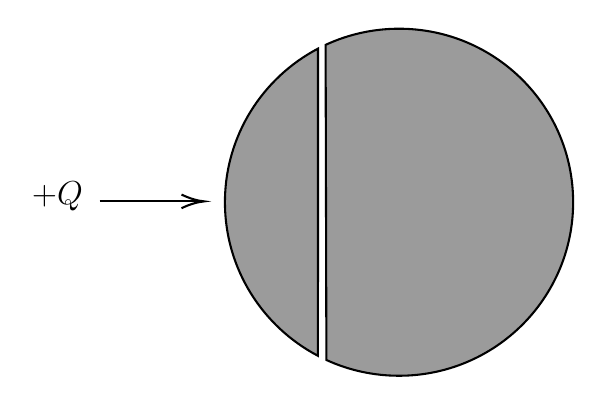
\begin{tikzpicture}[x=0.75pt,y=0.75pt,yscale=-1,xscale=1]
%uncomment if require: \path (0,470); %set diagram left start at 0, and has height of 470

%Shape: Chord [id:dp7672516414983406] 
\draw  [fill={rgb, 255:red, 155; green, 155; blue, 155 }  ,fill opacity=1 ] (300.99,285.19) .. controls (274.34,271.19) and (256.18,243.31) .. (256.18,211.2) .. controls (256.18,179.08) and (274.36,151.19) .. (301.02,137.19) -- cycle ;
%Shape: Chord [id:dp8357761441104918] 
\draw  [fill={rgb, 255:red, 155; green, 155; blue, 155 }  ,fill opacity=1 ] (304.68,135.38) .. controls (315.43,130.39) and (327.42,127.6) .. (340.06,127.6) .. controls (386.39,127.6) and (423.94,165.03) .. (423.94,211.2) .. controls (423.94,257.37) and (386.39,294.8) .. (340.06,294.8) .. controls (327.57,294.8) and (315.71,292.08) .. (305.06,287.2) -- cycle ;
%Straight Lines [id:da8177035752650788] 
\draw    (195.79,210.79) -- (244.18,210.79) ;
\draw [shift={(246.18,210.79)}, rotate = 180] [color={rgb, 255:red, 0; green, 0; blue, 0 }  ][line width=0.75]    (10.93,-3.29) .. controls (6.95,-1.4) and (3.31,-0.3) .. (0,0) .. controls (3.31,0.3) and (6.95,1.4) .. (10.93,3.29)   ;


% Text Node
\draw (161.64,200.09) node [anchor=north west][inner sep=0.75pt]    [font=\large] {$+Q$};


\end{tikzpicture}
\end{center}
\end{vd}

\begin{loigiai}
\begin{enumerate}[1)]
    \item Điện tích $+Q$ ở mảnh cắt bên trái sẽ tạo ra điện tích hưởng ứng làm thay đổi lại phân bố điện của phần trung hòa bên phải. Mặt phẳng cắt cách điện giữa hai phần có thể được coi như hai bản của một tụ phẳng vô hạn với khoảng cách giữa hai bản vô cùng nhỏ. Nếu chúng ta gọi điện tích trên hai bản của ``tụ'' lần lượt là $+q$ và $-q$ thì phân bố điện tích tổng thể của quả cầu được thể hiện như hình:
    \begin{center}
        \tikzset{every picture/.style={line width=0.75pt}} %set default line width to 0.75pt        
    
    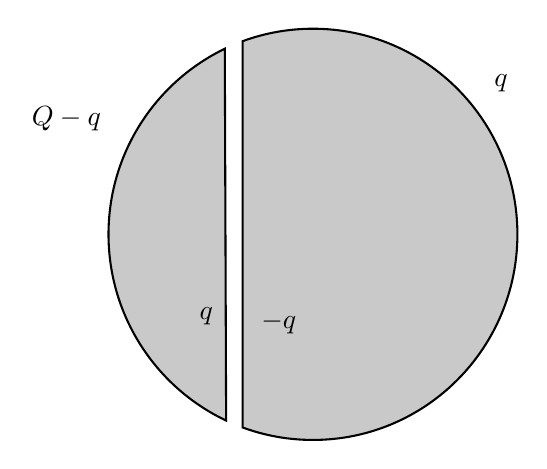
\begin{tikzpicture}[x=0.75pt,y=0.75pt,yscale=-1,xscale=1]
    %uncomment if require: \path (0,470); %set diagram left start at 0, and has height of 470
    
    %Shape: Chord [id:dp06257868663189114] 
    \draw  [fill={rgb, 255:red, 155; green, 155; blue, 155 }  ,fill opacity=0.54 ] (264.77,347.35) .. controls (231.29,331.53) and (208.1,297.3) .. (208.1,257.63) .. controls (208.1,218.22) and (230.99,184.18) .. (264.13,168.22) -- cycle ;
    %Shape: Chord [id:dp8231808665359597] 
    \draw  [fill={rgb, 255:red, 155; green, 155; blue, 155 }  ,fill opacity=0.54 ] (272.74,164.58) .. controls (283.3,160.69) and (294.71,158.57) .. (306.61,158.57) .. controls (361.01,158.57) and (405.11,202.92) .. (405.11,257.63) .. controls (405.11,312.35) and (361.01,356.7) .. (306.61,356.7) .. controls (294.71,356.7) and (283.3,354.58) .. (272.74,350.69) -- cycle ;
    
    
    % Text Node
    \draw (169.66,194.49) node [anchor=north west][inner sep=0.75pt]    {$Q-q$};
    % Text Node
    \draw (250.53,291.39) node [anchor=north west][inner sep=0.75pt]    {$q$};
    % Text Node
    \draw (280.26,293.74) node [anchor=north west][inner sep=0.75pt]    {$-q$};
    % Text Node
    \draw (392.56,179.14) node [anchor=north west][inner sep=0.75pt]    {$q$};
    
    
    \end{tikzpicture}
    \end{center}
    Dễ thấy, vì cả hai mảnh cắt đều làm từ kim loại nên chúng chỉ được tích điện bề mặt. Theo định luật bảo toàn điện tích, tổng điện tích của hai phần quả cầu đều không thay đổi lần lượt là $Q$ và $0$.\\
    Bây giờ chúng ta sẽ xem xét năng lượng của hệ. Vì khoảng cách giữa hai bản ``tụ''rất nhỏ nên điện dung của tụ là vô cùng lớn do đó chúng ta có thể bỏ qua phần năng lượng tích trữ trên tụ. Một cách lí luận tương tự có thể áp dụng để bỏ qua năng lượng tương tác giữa $+Q$ và $+q$, $-q$. Vì thế, năng lượng tích trữ trên quả cầu chỉ còn do các điện tích ở bề mặt cầu tương tác với nhau. Vì chúng ta đang tìm điều kiện cân bằng của quả cầu nên năng lượng tương tác này hiển nhiên phải cực tiểu. Vì tổng điện tích trên cả mặt cầu là  $+Q$ không đổi (do điện tích hưởng ứng triệt tiêu nhau) nên dễ thấy năng lượng tương tác sẽ là cực tiểu khi mật độ điện tích mặt là đều tại mọi điểm $-$ giống như một quả cầu đặc chưa bị cắt.\\
    Từ đây nhờ định luật bảo toàn điện tích ta dễ dàng tính được $+q= 3Q/4$ và hiển nhiên $-q=-3Q/4.$\\
    Chúng ta cũng có thể giải bài toán theo một hướng tiếp cận khác. Vì các vật dẫn kim loại là vật đẳng thế nên điện trường bên trong chúng lúc cân bằng tại mọi điểm bằng $0$. Vì khoảng cách giữa hai bản tụ vô cùng nhỏ mà điện trường ở vùng đó lại hữu hạn nên hiệu điện thế giữa hai mảnh cắt có thể được bỏ qua, vì thế nên cả quả cầu là đẳng thế! Và với một quả cầu mang điện tích bề mặt $Q$, cách duy nhất để thỏa mãn điều kiện đẳng thế chính là mật độ điện tích mặt mọi điểm đều bằng nhau và bằng $\sigma$. Mật độ đó là:
    $$\sigma= \dfrac{Q}{4\pi R^2} = \text{const}.$$
    Điện tích phân bố đồng đều trên toàn quả cầu sẽ tạo ra điện trường bằng không tại mọi nơi bên trong quả cầu (dĩ nhiên là ngoại trừ vùng cắt như đã nói ở trên). Bên ngoài quả cầu điện trường có thể tính theo định luật Coulomb với độ lớn:
    $$E(r)=\dfrac{1}{4\pi \varepsilon_0}\dfrac{Q}{r^2}~~~(r>R).$$
    Ở ngoài quả cầu, các đường sức điện có thể được biểu diễn gần đúng như hình sau:
    \begin{center}
            
    \tikzset{every picture/.style={line width=0.75pt}} %set default line width to 0.75pt        
    
    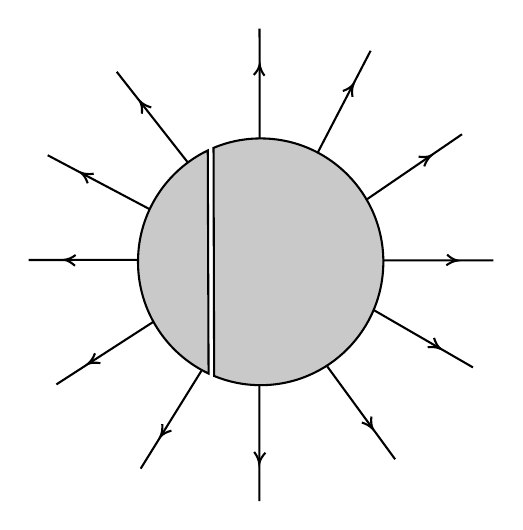
\begin{tikzpicture}[x=0.75pt,y=0.75pt,yscale=-0.6,xscale=0.6]
    %uncomment if require: \path (0,470); %set diagram left start at 0, and has height of 470
    
    %Shape: Chord [id:dp8024490198405001] 
    \draw  [fill={rgb, 255:red, 155; green, 155; blue, 155 }  ,fill opacity=0.54 ] (263.77,351.35) .. controls (230.29,335.53) and (207.1,301.3) .. (207.1,261.63) .. controls (207.1,222.22) and (229.99,188.18) .. (263.13,172.22) -- cycle ;
    %Shape: Chord [id:dp976723991371349] 
    \draw  [fill={rgb, 255:red, 155; green, 155; blue, 155 }  ,fill opacity=0.54 ] (267.75,170.15) .. controls (279.4,165.26) and (292.19,162.57) .. (305.61,162.57) .. controls (360.01,162.57) and (404.11,206.92) .. (404.11,261.63) .. controls (404.11,316.35) and (360.01,360.7) .. (305.61,360.7) .. controls (292.38,360.7) and (279.76,358.08) .. (268.24,353.32) -- cycle ;
    %Straight Lines [id:da6077534194083141] 
    \draw    (304.78,162.54) -- (304.69,74.47) ;
    \draw   (300.08,111.58) .. controls (302.63,108.89) and (304.21,106.12) .. (304.85,103.28) .. controls (305.17,106.19) and (306.45,109.15) .. (308.69,112.18) ;
    
    %Straight Lines [id:da6980317222556218] 
    \draw    (304.52,361.47) -- (304.6,453.88) ;
    \draw   (309.44,414.93) .. controls (306.77,417.77) and (305.1,420.67) .. (304.44,423.64) .. controls (304.1,420.6) and (302.76,417.49) .. (300.41,414.3) ;
    
    %Straight Lines [id:da5175943368997602] 
    \draw    (351.3,174.18) -- (393.88,92.17) ;
    \draw   (371.61,124.48) .. controls (375.28,123.2) and (378.1,121.4) .. (380.07,119.06) .. controls (378.96,121.93) and (378.71,125.3) .. (379.33,129.2) ;
    
    %Straight Lines [id:da7546902289036119] 
    \draw    (391,211.39) -- (467.28,159.23) ;
    \draw   (432.38,177.18) .. controls (436.23,177.79) and (439.57,177.54) .. (442.4,176.41) .. controls (440.08,178.4) and (438.26,181.26) .. (436.95,184.99) ;
    
    %Straight Lines [id:da6681376263532417] 
    \draw    (404.35,260.56) -- (492.42,260.48) ;
    \draw   (455.3,255.87) .. controls (458,258.42) and (460.77,260) .. (463.6,260.64) .. controls (460.7,260.96) and (457.74,262.24) .. (454.71,264.47) ;
    
    %Straight Lines [id:da8458738648687543] 
    \draw    (207.42,260.11) -- (119.35,260.19) ;
    \draw   (156.46,264.81) .. controls (153.76,262.27) and (151,260.67) .. (148.16,260.04) .. controls (151.06,259.72) and (154.03,258.43) .. (157.06,256.2) ;
    
    %Straight Lines [id:da67965590819354] 
    \draw    (219.22,309.97) -- (141.58,360.09) ;
    \draw   (176.94,343.06) .. controls (173.1,342.35) and (169.77,342.53) .. (166.91,343.58) .. controls (169.28,341.64) and (171.17,338.83) .. (172.58,335.13) ;
    
    %Straight Lines [id:da9312657735085952] 
    \draw    (258,349.23) -- (209.24,427.73) ;
    \draw   (233.93,397.22) .. controls (230.16,398.21) and (227.21,399.79) .. (225.08,401.97) .. controls (226.4,399.21) and (226.9,395.86) .. (226.59,391.92) ;
    
    %Straight Lines [id:da7341101052436314] 
    \draw    (216.27,219.29) -- (134.6,176.07) ;
    \draw   (166.73,198.59) .. controls (165.48,194.9) and (163.7,192.07) .. (161.38,190.09) .. controls (164.23,191.22) and (167.61,191.49) .. (171.52,190.91) ;
    
    %Straight Lines [id:da3903773796918495] 
    \draw    (247.06,181.8) -- (190.04,109.09) ;
    \draw   (210.23,142.74) .. controls (210.59,138.85) and (210.12,135.54) .. (208.81,132.79) .. controls (210.95,134.98) and (213.92,136.6) .. (217.73,137.67) ;
    
    %Straight Lines [id:da785443064340573] 
    \draw    (396.07,300.2) -- (476.08,346.44) ;
    \draw   (444.81,322.74) .. controls (445.92,326.47) and (447.59,329.37) .. (449.84,331.43) .. controls (447.03,330.2) and (443.67,329.8) .. (439.74,330.24) ;
    
    %Straight Lines [id:da17633506452078396] 
    \draw    (359.03,345.59) -- (413.57,420.19) ;
    \draw   (394.52,385.87) .. controls (394.04,389.74) and (394.4,393.07) .. (395.61,395.86) .. controls (393.55,393.6) and (390.63,391.88) .. (386.86,390.69) ;
    \end{tikzpicture}
    \end{center}
    \item Lực tương tác giữa hai mảnh cắt bao gồm hai thành phần: Lực hút giữa hai bản ``tụ'' và lực đẩy giữa các điện tích dương bề mặt 
    Gọi bề dày của phần bị cắt bên trái là $h$ (mà ở trong bài này $h = R/2$), thành phần lực hút giữa hai bản tụ là:
    $$F_{attr}=\dfrac{1}{2}qE=\dfrac{q^2}{2\varepsilon_0 A},$$
    Trong đó $A$ là tiết diện mặt cắt $A=\pi r^2$ và $r$ là bán kính mặt cắt $r=\sqrt{2Rh-h^2}$.
    \\Tổng điện tích của ``tụ'' là:
    $$q=\sigma (4\pi R^2-2 \pi Rh)=\dfrac{Q}{4\pi R^2}(4\pi R^2-2\pi Rh)=Q(1-\dfrac{h}{2R}),$$
    và do đó ta có thành phần lực hút: 
    $$F_{attr}=\dfrac{Q^2(2R-h)}{8\pi \varepsilon_0 R^2 h}.$$
    Mật độ điện tích trên bề mặt quả cầu là $\sigma=\dfrac{Q}{4\pi R^2},$
    do đó điện tích của một vùng diện tích $\Delta A$ là $\Delta Q=\sigma \Delta A$.\\Cường độ điện trường có độ lớn là $E$ ở bên ngoài quả cầu và bằng $0$ ở ngay bên trong quả cầu do đó có thể coi điện trường trung bình tại vùng này là $E/2$, và lực tác dụng vào vùng diện tích nhỏ đó là $E \Delta Q/2$, hướng ra ngoài bề mặt quả cầu.
    Vì lực tác dụng lên diện tích $\Delta A$ là lực vuông góc nên ta có thể đặt:
    $$p=\dfrac{E\Delta Q}{2\Delta A}=\dfrac{\sigma E}{2}=\dfrac{Q}{4\pi R^2} \dfrac{Q}{8\pi \varepsilon_0 R^2}=\dfrac{Q^2}{32 \pi^2\varepsilon_0 R^4}$$
    là áp suất điện tác dụng lên bề mặt ngoài quả cầu. Vì vậy quả cầu lúc này có thể coi như một quả bóng chứa đầy khí ở áp suất $p$. Do tính chất áp suất, lực giữa hai mảnh cắt tác dụng lên nhau chính bằng áp suất nhân với hình chiếu của chúng lên mặt phẳng, mà ở đây diện tích hình chiếu đấy chính bằng diện tích bản tụ:
    $$F=p\pi r^2.$$
    Do đó, thành phần lực đẩy giữa hai mảnh cắt là:
    $$F_{rep}=p\pi r^2=\dfrac{Q^2}{32\pi^2\varepsilon_0R^4}\pi (2Rh-h^2)=\dfrac{Q^2(2R-h)h}{32\pi \varepsilon_0R^4}.$$
    Dễ thấy, trong trường hợp $0<h<2R$ (có tính vật lý) thì thành phần lực hút luôn lớn hơn thành phần lực đẩy, do đó hai mảnh cắt luôn hút nhau với một lực có độ lớn bằng:
    $$F_{net}=F_{attr}-F_{rep}=\dfrac{Q^2(2R-h)(4R^2-h^2)}{32\pi \varepsilon_0 R^4h}.$$
    Trong trường hợp cụ thể của bài toán này, ta có h=R/2, do đó hai mảnh cắt hút nhau bởi một lực có độ lớn:
    $$F_{net}^{(h=R/2)}=\dfrac{45Q^2}{128\pi \varepsilon_0 R^2}.$$

    \end{enumerate}
\end{loigiai}


\begin{vd}[Mặt đẳng thế của vòng tròn tích điện]
    \begin{enumerate}[1)]
    \setlength{\itemsep}{0pt}
        \item Một vòng bán kính $R$ có điện tích $Q$ phân bố đều trên chu vi của nó. Chiếc vòng nằm trong mặt phẳng $xy$, tâm vòng trùng với gốc tọa độ. Tìm cường độ điện trường tại một điểm nằm trên trục $z$. Với giá trị nào của $z$ thì cường độ điện trường đạt giá trị cực đại? \label{ca7}
        \item Phác thảo các mặt đẳng thế của chiếc vòng trong không gian. Do tính đối xứng của hệ, bạn chỉ cần vẽ phần giao của các mặt đẳng thế và một mặt phẳng đi qua trục $z$, bạn có thể thể hiện chiếc vòng trong mặt phẳng này bằng hai điểm giao nhau của vòng và mặt phẳng. Hãy chú ý đến hình dạng của các đường đẳng thế tại những vị trí gần và xa vòng, và sự thay đổi của các đường đẳng thế khi di chuyển từ gần ra xa.
        \item Có một vị trí trên trục $z$ mà tại đó đường đẳng thế thay đổi từ cong xuống dưới sang cong lên trên. Tìm tọa độ của vị trí này. Lí giải tại sao giá trị $z$ mà bạn tìm được lại giống với giá trị $z$ mà tại đó cường độ điện trường cực đại bạn tìm được ở phần \ref{ca7}. \\
        \textit{Gợi ý:Cường độ điện trường của $\ot{E}$ bằng không.}
    \end{enumerate}
    \end{vd}
    \begin{loigiai}
    \begin{enumerate}[1)]
    \setlength{\itemsep}{0pt}
        \item \hfill\\
        \begin{center}
            

\tikzset{every picture/.style={line width=0.75pt}} %set default line width to 0.75pt        

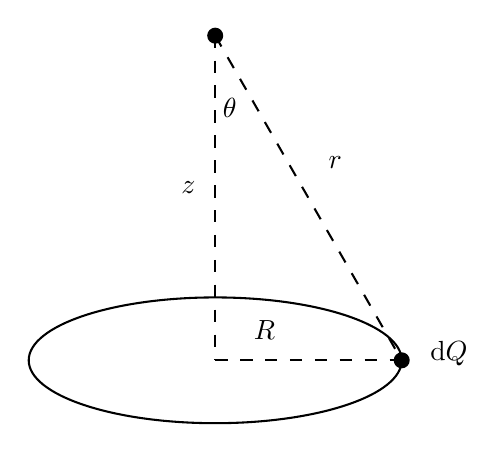
\begin{tikzpicture}[x=0.75pt,y=0.75pt,yscale=-1,xscale=1]
%uncomment if require: \path (0,300); %set diagram left start at 0, and has height of 300

%Shape: Ellipse [id:dp7526869081481533] 
\draw   (267,172) .. controls (267,155.27) and (307.23,141.7) .. (356.85,141.7) .. controls (406.48,141.7) and (446.71,155.27) .. (446.71,172) .. controls (446.71,188.73) and (406.48,202.3) .. (356.85,202.3) .. controls (307.23,202.3) and (267,188.73) .. (267,172) -- cycle ;
%Straight Lines [id:da7631985553546445] 
\draw  [dash pattern={on 4.5pt off 4.5pt}]  (356.85,172) -- (446.71,172) ;
\draw [shift={(446.71,172)}, rotate = 0] [color={rgb, 255:red, 0; green, 0; blue, 0 }  ][fill={rgb, 255:red, 0; green, 0; blue, 0 }  ][line width=0.75]      (0, 0) circle [x radius= 3.35, y radius= 3.35]   ;
%Straight Lines [id:da7311587190761697] 
\draw  [dash pattern={on 4.5pt off 4.5pt}]  (356.85,15.59) -- (356.85,172) ;
\draw [shift={(356.85,15.59)}, rotate = 90] [color={rgb, 255:red, 0; green, 0; blue, 0 }  ][fill={rgb, 255:red, 0; green, 0; blue, 0 }  ][line width=0.75]      (0, 0) circle [x radius= 3.35, y radius= 3.35]   ;
%Straight Lines [id:da9294712862450247] 
\draw  [dash pattern={on 4.5pt off 4.5pt}]  (356.85,15.59) -- (446.71,172) ;

% Text Node
\draw (359,44.4) node [anchor=north west][inner sep=0.75pt]    {$\theta $};
% Text Node
\draw (339,84.4) node [anchor=north west][inner sep=0.75pt]    {$z$};
% Text Node
\draw (410,72.4) node [anchor=north west][inner sep=0.75pt]    {$r$};
% Text Node
\draw (374,151.4) node [anchor=north west][inner sep=0.75pt]    {$R$};
% Text Node
\draw (459,161.4) node [anchor=north west][inner sep=0.75pt]    {$\mathrm{d} Q$};


\end{tikzpicture}

        \end{center}
        Tại một điểm nằm trên trục $z$, điện trường gây ra bởi một phần tử nhỏ có điện tích $\dd Q$ nằm trên vòng là $\dfrac{\dd Q}{4\pi\varepsilon_0 r^2}$. Do tính đối xứng, từ trường do cả vòng gây ra tại điểm đó có phương dọc theo trục $z$, vậy nên chỉ có thành phần dọc theo trục $z$ của điện trường do $\dd Q$ gây ra đóng góp vào điện trường cuối cùng. Ta có:
        \begin{equation}
            \dd E=\dfrac{\dd Q}{4\pi\varepsilon_0 r^2}\cos\theta=\dfrac{\dd Q}{4\pi\varepsilon_0 r^2}\dfrac{z}{r}.
        \end{equation}
        Tích phân trên toàn bộ vòng, ta có:
        \begin{equation}
            E(z)=\int \dfrac{\dd Q}{4\pi\varepsilon_0 r^2}\dfrac{z}{r}=\dfrac{Qz}{4\pi\varepsilon_0r^3}= \dfrac{Qz}{4\pi\varepsilon_0\tron{R^2+z^2}^\frac{3}{2}}.   
        \end{equation}
        Khi $z\rightarrow\infty$ thì $E(z)\rightarrow\dfrac{Q}{4\pi\varepsilon_0 z^2}$, điều này là hợp lí vì khi $z$ lớn thì ta có thể coi vòng như là một điện tích điểm. Nếu $z=0$ thì $E(z)=0$, tại đây do đối xứng nên điện trường do từng phần tử trên vòng triệt tiêu lẫn nhau.\\
        Ta có:
        \begin{equation}
            \begin{aligned}
               \dfrac{\dd E(z)}{\dd z}= \dfrac{Q}{4\pi\varepsilon_0}\dfrac{\tron{z^2+R^2}^\frac{3}{2}-3z^2\tron{R^2+z^2}^\frac{1}{2}}{\tron{R^2+z^2}^3}.
            \end{aligned}
        \end{equation}
        Khi cường độ điện trường đạt cực trị:
        \begin{equation}
            \begin{aligned}
               \dfrac{\dd E(z)}{\dd z}=0&\Leftrightarrow \tron{z^2+R^2}^\frac{3}{2}-3z^2\tron{R^2+z^2}^\frac{1}{2}=0\\
               &\Leftrightarrow R^2-2z^2=0\\
               &\Leftrightarrow z=\dfrac{R}{\sqrt{2}}.
            \end{aligned}
        \end{equation}
        \item \hfil \\
        \begin{center}
            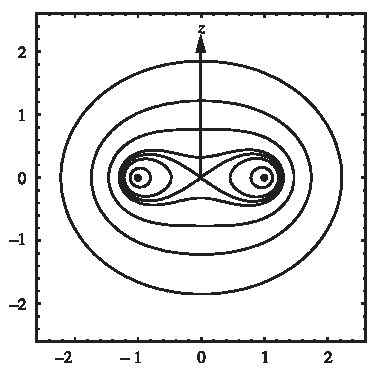
\includegraphics[scale=1]{Anh/c3.pdf}
        \end{center}
        Các đường đẳng thế được phác họa như trên hình. Điểm giao nhau giữa vòng và mặt phẳng được biểu diễn bằng hai dấu chấm, trên hình bán kính vòng dây được chọn bằng một đơn vị độ dài $R=1$. Toàn bộ mặt đẳng thế trong không gian có thể thu được bằng cách xoay các đường đẳng thế quanh trục $z$ để tạo thành các mặt đối xứng tròn xoay.\\
        Trên hình, ta có thể thấy rằng tại các vị trí gần vòng dây, đường đẳng thế gần giống với những vòng tròn bao quanh vòng dây (tương ứng với mặt đẳng thế là mặt hình xuyến trong không gian). Tại những điểm ở xa vòng dây, đường đẳng thế là những đường tròn tâm trùng với tâm vòng dây (trong không gian mặt đẳng thế là những mặt cầu bao quanh vòng dây). Sự chuyển tiếp giữa hai dạng mặt đẳng thế xảy ra khi mặt đẳng thế đi qua gốc tọa độ như trên hình. 
        \item \hfill \\
        \begin{center}
            

\tikzset{every picture/.style={line width=0.75pt}} %set default line width to 0.75pt        

\begin{tikzpicture}[x=0.75pt,y=0.75pt,yscale=-1,xscale=1]
%uncomment if require: \path (0,222); %set diagram left start at 0, and has height of 222

%Shape: Arc [id:dp21376736629493287] 
\draw  [draw opacity=0] (455.75,127.09) .. controls (439.25,140.2) and (399.45,149.44) .. (352.97,149.44) .. controls (311.61,149.44) and (275.54,142.12) .. (256.47,131.27) -- (352.97,113.57) -- cycle ; \draw   (455.75,127.09) .. controls (439.25,140.2) and (399.45,149.44) .. (352.97,149.44) .. controls (311.61,149.44) and (275.54,142.12) .. (256.47,131.27) ;
%Straight Lines [id:da6782292671629595] 
\draw    (352.97,19.58) -- (352.97,187.34) ;
\draw [shift={(352.97,16.58)}, rotate = 90] [fill={rgb, 255:red, 0; green, 0; blue, 0 }  ][line width=0.08]  [draw opacity=0] (10.72,-5.15) -- (0,0) -- (10.72,5.15) -- (7.12,0) -- cycle    ;
%Straight Lines [id:da24086650305652246] 
\draw    (224,187.34) -- (478.95,187.34) ;
\draw [shift={(481.95,187.34)}, rotate = 180] [fill={rgb, 255:red, 0; green, 0; blue, 0 }  ][line width=0.08]  [draw opacity=0] (10.72,-5.15) -- (0,0) -- (10.72,5.15) -- (7.12,0) -- cycle    ;
%Straight Lines [id:da18947837970533232] 
\draw    (311.41,147.08) -- (318.48,100.82) ;
\draw [shift={(318.79,98.84)}, rotate = 458.7] [fill={rgb, 255:red, 0; green, 0; blue, 0 }  ][line width=0.08]  [draw opacity=0] (12,-3) -- (0,0) -- (12,3) -- cycle    ;
%Shape: Boxed Line [id:dp5843424318289914] 
\draw    (393.84,147.08) -- (386.76,100.82) ;
\draw [shift={(386.46,98.84)}, rotate = 441.3] [fill={rgb, 255:red, 0; green, 0; blue, 0 }  ][line width=0.08]  [draw opacity=0] (12,-3) -- (0,0) -- (12,3) -- cycle    ;

% Text Node
\draw (363.68,10.89) node [anchor=north west][inner sep=0.75pt]    {$z$};
% Text Node
\draw (487.1,189.64) node [anchor=north west][inner sep=0.75pt]    {$x$};
% Text Node
\draw (295.88,81.84) node [anchor=north west][inner sep=0.75pt]    {$\vec{E}$};
% Text Node
\draw (394.01,81.84) node [anchor=north west][inner sep=0.75pt]    {$\vec{E}$};
% Text Node
\draw (463.71,157.57) node   [align=left] {\begin{minipage}[lt]{95.03pt}\setlength\topsep{0pt}
Đường đẳng thế
\end{minipage}};


\end{tikzpicture}

        \end{center}
        Xét một điểm nằm trên trục $z$ mà tại đó đường đẳng thế có mặt lõm hướng lên trên như hình. Điện trường vuông góc với mặt đẳng thế như trên hình. Ta thấy về phía bên trái điểm đang xét, vector cường độ điện trường nghiêng về phía bên phải, tức là thành phần điện trường theo phương $x$ có giá trị dương. Tương tự như vậy, về phía bên phải điểm đang xét, thành phần điện trường dọc theo trục $x$ có giá trị âm. Ta thấy rằng khi đi qua vị trí điểm đó từ trái qua phải, thành phần điện trường dọc theo trục giảm đi, do đó $\dfrac{\partial E_x}{\partial x}<0$. Do tính đối xứng nên ta cũng có $\dfrac{\partial E_y}{\partial y}<0$. \\
        Lập luận tương tự, tại một điểm mà mặt đẳng thể có mặt lõm hướng lên trên thì $\dfrac{\partial E_x}{\partial x}>0$, $\dfrac{\partial E_y}{\partial y}>0$. Vì $\dfrac{\partial E_x}{\partial x}$ và $\dfrac{\partial E_y}{\partial y}$ là liên tục, nên tại điểm mà mặt đẳng thế thay đổi từ có mặt lõm hướng xuống dưới sang hướng lên trên thì $\dfrac{\partial E_x}{\partial x}$ và $\dfrac{\partial E_y}{\partial y}$ chuyển từ âm sang dương và có giá trị bằng không.\\
        Ta có $\nabla\cdot \ot{E}=\dfrac{\rho}{\varepsilon_0}$. Do tại điểm xảy ra sự chuyển tiếp, mật độ điện tích bằng không nên ta có:
        \begin{equation}
            \nabla\cdot \ot{E}=\dfrac{\rho}{\varepsilon_0}=0\Leftrightarrow \dfrac{\partial E_x}{\partial x}+\dfrac{\partial E_y}{\partial y}+\dfrac{\partial E_z}{\partial z}=0.
        \end{equation}
        Mà như ta đã biết, $\dfrac{\partial E_x}{\partial x}=0$ và $\dfrac{\partial E_y}{\partial y}=0$, vậy nên $\dfrac{\partial E_z}{\partial z}=0$. Từ đó ta thấy được tại điểm chuyển tiếp thì thành phần điện trường theo phương $z$ đạt cực trị, đây chính là điểm mà ta đã xác định ở phần (\ref{ca7}).
    \end{enumerate}
    \end{loigiai}
  
\begin{vd}[Lấp và đầy]%câu 2
%USAPhO 2018
Điện thế tại tâm của khối lập phương với mật độ điện khối $\rho$ và cạnh $a$ cho bởi
$$\Phi  \approx \dfrac{{0,1894\rho {a^2}}}{{{\varepsilon_0}}}.$$
Bạn không cần phải chứng minh công thức này. Trong toàn bộ bài toán, các kết quả tính số phải viết với ba chữ số có nghĩa.
\begin{enumerate}[1)]
    \item Tìm điện thế tại đỉnh của khối lập phương. Đáp số biểu diễn qua $\rho ,a,{\varepsilon _0}$ và các giá trị số cần thiết.
    \item Tìm điện thế tại đỉnh kim tự tháp với đáy hình vuông có cạnh $a$, chiều cao $a/2$, và tích điện đều với mật độ điện khối $\rho$. Đáp số biểu diễn qua $\rho ,a,{\varepsilon _0}$ và các giá trị số cần thiết.
    \item Tìm điện thế gây bởi một bản mỏng hình vuông cạnh $a$ có mật độ điện mặt $\sigma$ tại một điểm nằm cách tâm của nó ở độ cao $a/2$. Đáp số biểu diễn qua $\sigma ,a,{\varepsilon _0}$ và các giá trị số cần thiết.
    \item Ký hiệu $E\tron{z}$ là điện trường ở độ cao $z$ từ tâm hình vuông với mật độ điện mặt $\sigma$ và cạnh $a$. Nếu điện thế tại tâm hình vuông có biểu thức gần đúng $\dfrac{{0,281a\sigma }}{{{\varepsilon _0}}}$, đánh giá $E\tron{a/2}$ nếu giả thiết $E\tron{z}$ tuyến tính trong khoảng $0<z<a/2$. Đáp số biểu diễn qua $\sigma ,a,{\varepsilon _0}$ và các giá trị số cần thiết.
\end{enumerate}
\end{vd}
\begin{loigiai}

\begin{enumerate}[1)]

\item Bằng phương pháp phân tích thứ nguyên, đáp án sẽ có dạng:
$$\Phi_c\tron{a,\rho}\approx\dfrac{C\rho a^2}{\varepsilon_0},$$
với $C$ là một hằng số không thứ nguyên. Lưu ý rằng một hình lập phương có cạnh $a$ gồm $8$ hình lập phương có cạnh $a/2$, với mỗi hình lập phương có một đỉnh ở tâm của hình lập phương lớn. Do đó:
$$\dfrac{{0,1894\rho {a^2}}}{{{\varepsilon_0}}}=8\dfrac{C\rho \tron{a/2}^2}{\varepsilon_0},$$
nên $C=0,1894/2=0.0947.$
\item Hình lập phương cạnh $a$ sẽ bao gồm $6$ hình kim tự tháp như vậy. Vì vậy chúng ta chỉ cần tính toán đơn giản $0.1894/6$ và được kết quả:
$$\Phi_p\tron{a,\rho}  \approx \dfrac{{0,0316\rho {a^2}}}{{{\varepsilon_0}}}.$$
\item Gọi điện thế gây bởi hình vuông như vậy là $\Phi_s\tron{a,\sigma}$. Lưu ý rằng việc thêm một bản hình vuông có độ dày $\dd z$ rất nhỏ và độ dài cạnh $a$ vào một kim tự tháp đáy vuông với độ dài cạnh đáy là $a$, chiều cao $a/2$ sẽ tạo ra một kim tự tháp đáy vuông có độ dài cạnh đáy $a+2\dd z$ và chiều cao $a/2+\dd z.$\\
Mật độ điện tích mặt của đĩa vuông có độ dày $\dd z$ liên hệ với mật độ điện tích khối là $\sigma=\rho \dd z$. Theo nguyên lý chồng chất:
$$\Phi_{s}(a, \rho \dd z)=\Phi_{p}(a+2 \dd z, \rho)-\Phi_{p}(a, \rho) \approx \frac{0,0316 \rho\left((a+2 \dd z)^{2}-a^{2}\right)}{\varepsilon_{0}}=\frac{0,126 a \rho \dd z}{\varepsilon_{0}}.$$
Do đó ta có:
$$\Phi_s\tron{a,\sigma}\approx\dfrac{0,126a\sigma}{\varepsilon_0}.$$
\item Hiệu điện thế giữa hai điểm có độ cao $0$ và $a/2$ là:
$$\Delta\Phi = \tron{0,281-0,126}\dfrac{a\sigma}{\varepsilon_0}=\dfrac{0,155a\sigma}{\varepsilon_0}.$$
Mặt khác, ta có:
$$\Delta \Phi=\int_{0}^{a / 2} E(z) d z \approx \dfrac{a}{2} \dfrac{E(0)+E(a / 2)}{2},$$
trong đó, ta đã coi gần đúng $E\tron{z}$ như một hàm tuyến tính, và $E\tron{0}=\sigma/2\varepsilon_0$ theo định luật Gauss. Giải phương trình tìm $E\tron{a/2}$ ta được:
$$E\tron{a/2}\approx\dfrac{0,119\sigma}{\varepsilon_0},$$
với chữ số có nghĩa cuối cùng không quan trọng. Một cách tình cờ, giá trị thực tế chính xác là $\sigma/6\varepsilon_0$, và giá trị thực tế này có một cách chứng minh khá là mượt mà mà không cần tính toán.
\end{enumerate}
\end{loigiai}


\begin{vd}[Bản chất của lưỡng cực từ]%câu 7
%USAPhO 2015

\begin{enumerate}[1)]
    \item Một lưỡng cực ``Gilbert'' bao gồm một cặp đơn cực từ, hai cực có độ lớn $q_m$ bằng nhau và trái dấu, cách nhau một khoảng $d$ nhỏ. Trong phần này, giả sử rằng $-q_m$ ở tọa độ $z=0$ còn $q_m$ ở tọa độ $z=d$.
    \begin{center}
        

% Gradient Info
  
\tikzset {_vc3yyirl7/.code = {\pgfsetadditionalshadetransform{ \pgftransformshift{\pgfpoint{0 bp } { 0 bp }  }  \pgftransformscale{1 }  }}}
\pgfdeclareradialshading{_z372z9q49}{\pgfpoint{0bp}{0bp}}{rgb(0bp)=(1,1,1);
rgb(1.1607142857142858bp)=(1,1,1);
rgb(25bp)=(0,0,0);
rgb(400bp)=(0,0,0)}

% Gradient Info
  
\tikzset {_imxquv36r/.code = {\pgfsetadditionalshadetransform{ \pgftransformshift{\pgfpoint{0 bp } { 0 bp }  }  \pgftransformscale{1 }  }}}
\pgfdeclareradialshading{_may1wpven}{\pgfpoint{0bp}{0bp}}{rgb(0bp)=(1,1,1);
rgb(1.1607142857142858bp)=(1,1,1);
rgb(25bp)=(0,0,0);
rgb(400bp)=(0,0,0)}
\tikzset{every picture/.style={line width=0.75pt}} %set default line width to 0.75pt        

\begin{tikzpicture}[x=0.75pt,y=0.75pt,yscale=-1,xscale=1]
%uncomment if require: \path (0,360); %set diagram left start at 0, and has height of 360

%Straight Lines [id:da1763404976584506] 
\draw  [dash pattern={on 4.5pt off 4.5pt}]  (141,220) -- (513,220) ;
%Shape: Circle [id:dp21724950617475192] 
\path  [shading=_z372z9q49,_vc3yyirl7] (217,218) .. controls (217,212.48) and (221.48,208) .. (227,208) .. controls (232.52,208) and (237,212.48) .. (237,218) .. controls (237,223.52) and (232.52,228) .. (227,228) .. controls (221.48,228) and (217,223.52) .. (217,218) -- cycle ; % for fading 
 \draw   (217,218) .. controls (217,212.48) and (221.48,208) .. (227,208) .. controls (232.52,208) and (237,212.48) .. (237,218) .. controls (237,223.52) and (232.52,228) .. (227,228) .. controls (221.48,228) and (217,223.52) .. (217,218) -- cycle ; % for border 

%Shape: Circle [id:dp6921675875101942] 
\path  [shading=_may1wpven,_imxquv36r] (301,218) .. controls (301,212.48) and (305.48,208) .. (311,208) .. controls (316.52,208) and (321,212.48) .. (321,218) .. controls (321,223.52) and (316.52,228) .. (311,228) .. controls (305.48,228) and (301,223.52) .. (301,218) -- cycle ; % for fading 
 \draw   (301,218) .. controls (301,212.48) and (305.48,208) .. (311,208) .. controls (316.52,208) and (321,212.48) .. (321,218) .. controls (321,223.52) and (316.52,228) .. (311,228) .. controls (305.48,228) and (301,223.52) .. (301,218) -- cycle ; % for border 


% Text Node
\draw (206,174.4) node [anchor=north west][inner sep=0.75pt]    {$-q_{m}$};
% Text Node
\draw (299,175.4) node [anchor=north west][inner sep=0.75pt]    {$q_{m}$};
% Text Node
\draw (205,243.4) node [anchor=north west][inner sep=0.75pt]    {$z=0$};
% Text Node
\draw (292,242.4) node [anchor=north west][inner sep=0.75pt]    {$z=d$};
% Text Node
\draw (489,194.4) node [anchor=north west][inner sep=0.75pt]    {$z$};


\end{tikzpicture}

    \end{center}
    Giả sử rằng các đơn cực từ hoạt động như các đơn cực điện dưới tác dụng của một lực giống như lực Coulomb:
    $$F=\dfrac{\mu_0}{4\pi}\dfrac{q_{m_1}q_{m_2}}{r^2},$$
    và độ lớn cảm ứng từ có công thức:
    $$B=\dfrac{F}{q_m}.$$
    \begin{enumerate}[a)]
        \item Thứ nguyên của đại lượng $q_m$ là gì?
        \item Viết biểu thức chính xác của cảm ứng từ $B\tron{z}$ dọc theo trục $z$ như một hàm của $z$ với $z>d$. Hãy biểu diễn kết quả theo $q_m$, $d$, $z$, và các hằng số cơ bản cần thiết.
        \item Tìm giới hạn của biểu thức$B\tron{z}$ vừa tìm khi $d\rightarrow 0$, giả sử rằng tích $q_m d=p_m$ được giữ không đổi, kết quả chỉ giữ tới bậc nhỏ nhất khác không. Biểu diễn kết quả theo $q_m$, $z$ và các hằng số cơ bản cần thiết.
    \end{enumerate}
    \item Một lưỡng cực ``Ampère'' là một lực cực từ tạo bởi dòng điện $I$ chạy trong vòng tròn bán kính $r$ nhỏ. Giả sử rằng trục $z$ trùng với trục đối xứng của vòng dây dẫn, và vòng dây nằm trong mặt phẳng $xy$ tại $z=0$.
    \begin{center}
        

\tikzset{every picture/.style={line width=0.75pt}} %set default line width to 0.75pt        

\begin{tikzpicture}[x=0.75pt,y=0.75pt,yscale=-1,xscale=1]
%uncomment if require: \path (0,369); %set diagram left start at 0, and has height of 369

%Shape: Ellipse [id:dp042219169506113374] 
\draw  [line width=1.5]  (280.5,186) .. controls (290.16,186) and (298,210.4) .. (298,240.5) .. controls (298,270.6) and (290.16,295) .. (280.5,295) .. controls (270.84,295) and (263,270.6) .. (263,240.5) .. controls (263,210.4) and (270.84,186) .. (280.5,186) -- cycle ;
%Straight Lines [id:da3414436567613002] 
\draw  [dash pattern={on 4.5pt off 4.5pt}]  (161,240) -- (533,240) ;
%Curve Lines [id:da8131452990600614] 
\draw    (299,192) .. controls (282.35,163.32) and (265.7,182.57) .. (260.13,194.32) ;
\draw [shift={(259,197)}, rotate = 289.98] [fill={rgb, 255:red, 0; green, 0; blue, 0 }  ][line width=0.08]  [draw opacity=0] (10.72,-5.15) -- (0,0) -- (10.72,5.15) -- (7.12,0) -- cycle    ;

% Text Node
\draw (305,167.4) node [anchor=north west][inner sep=0.75pt]    {$I$};
% Text Node
\draw (507,215.4) node [anchor=north west][inner sep=0.75pt]    {$z$};


\end{tikzpicture}

    \end{center}
    \begin{enumerate}[a)]
        \item Viết biểu thức chính xác của cảm ứng từ $B\tron{z}$ dọc theo trục $z$ như một hàm của $z$ với $z>0$. Hãy biểu diễn kết quả theo $I$, $r$, $z$ và các hằng số cơ bản cần thiết.
        \item Cho $kIr^\gamma$ có thứ nguyên giống với $p_m$ (ở phần trước), trong đó $k$ và $\gamma$ là những hằng số không thứ nguyên. Tìm giá trị của $\gamma$.
        \item Tìm giới hạn của biểu thức $B\tron{z}$ vừa tìm ở phần 2) a) khi $r\rightarrow 0$, giả sử rằng tích $kIr^\gamma=p'_m$ được giữ không đổi, kết quả chỉ giữ tới bậc nhỏ nhất khác không. Biểu diễn kết quả theo $k$, $p'_m$, $z$ và các hằng số cơ bản cần thiết.
        \item Giả sử rằng hai lưỡng cực từ có độ lớn bằng nhau, $p_m=p'_m$. Tìm hằng số $k$ ở phần 2) b).
    \end{enumerate}
    \item Giờ ta thử so sánh hai loại lưỡng cực bằng cách xây dựng một mô hình nam châm vật lý được cấu tạo bởi các lưỡng cực từ cực nhỏ được sắp xếp dày đặc.
    \begin{center}
        

\tikzset{every picture/.style={line width=0.75pt}} %set default line width to 0.75pt        

\begin{tikzpicture}[x=0.75pt,y=0.75pt,yscale=-1,xscale=1]
%uncomment if require: \path (0,438); %set diagram left start at 0, and has height of 438

%Shape: Can [id:dp4163311919612256] 
\draw   (355.75,168.33) -- (258.78,168.33) .. controls (245.31,168.33) and (234.39,138.34) .. (234.39,101.34) .. controls (234.39,64.35) and (245.31,34.35) .. (258.78,34.35) -- (355.75,34.35) .. controls (369.23,34.35) and (380.15,64.35) .. (380.15,101.34) .. controls (380.15,138.34) and (369.23,168.33) .. (355.75,168.33) .. controls (342.28,168.33) and (331.36,138.34) .. (331.36,101.34) .. controls (331.36,64.35) and (342.28,34.35) .. (355.75,34.35) ;
%Straight Lines [id:da980952439721346] 
\draw  [dash pattern={on 4.5pt off 4.5pt}]  (354.92,101.73) -- (425,101.73) ;
%Straight Lines [id:da1079828190551615] 
\draw  [dash pattern={on 4.5pt off 4.5pt}]  (186.33,101.34) -- (234.39,101.34) ;
%Straight Lines [id:da46891481834208926] 
\draw    (258.61,26.22) -- (354.72,26.22) ;
\draw [shift={(357.72,26.22)}, rotate = 180] [fill={rgb, 255:red, 0; green, 0; blue, 0 }  ][line width=0.08]  [draw opacity=0] (7.14,-3.43) -- (0,0) -- (7.14,3.43) -- (4.74,0) -- cycle    ;
\draw [shift={(255.61,26.22)}, rotate = 0] [fill={rgb, 255:red, 0; green, 0; blue, 0 }  ][line width=0.08]  [draw opacity=0] (7.14,-3.43) -- (0,0) -- (7.14,3.43) -- (4.74,0) -- cycle    ;
%Straight Lines [id:da1280330733442938] 
\draw    (354.92,37.35) -- (354.92,98.73) ;
\draw [shift={(354.92,101.73)}, rotate = 270] [fill={rgb, 255:red, 0; green, 0; blue, 0 }  ][line width=0.08]  [draw opacity=0] (7.14,-3.43) -- (0,0) -- (7.14,3.43) -- (4.74,0) -- cycle    ;
\draw [shift={(354.92,34.35)}, rotate = 90] [fill={rgb, 255:red, 0; green, 0; blue, 0 }  ][line width=0.08]  [draw opacity=0] (7.14,-3.43) -- (0,0) -- (7.14,3.43) -- (4.74,0) -- cycle    ;

% Text Node
\draw (303.27,4.68) node [anchor=north west][inner sep=0.75pt]    {$L$};
% Text Node
\draw (361.04,80.58) node [anchor=north west][inner sep=0.75pt]    {$R$};
% Text Node
\draw (401.78,83.68) node [anchor=north west][inner sep=0.75pt]    {$z$};


\end{tikzpicture}

    \end{center}
    Một hình trụ làm bằng vật liệu từ tính có bán kính $R$ và chiều dài $L$. Nó được cấu tạo bởi $N$ lưỡng cực từ với tất cả đều là loại Ampère hoặc tất cả đều là loại Gilbert. $N$ rất lớn. Trục quay của hình trụ và tất cả các lưỡng cực đều thẳng hàng với trục $z$ và tất cả đều hướng theo cùng một hướng như đã xác định ở trên để từ trường bên ngoài hình trụ giống nhau với hai loại lưỡng cực đã được xác định trước đó. Hình dưới đây là mô hình của hai lưỡng cực; chúng là các hình lập phương với cạnh $d\ll R$ và $d\ll L$ với thể tích $v_m=d^3$.
    \begin{center}
        

\tikzset{every picture/.style={line width=0.75pt}} %set default line width to 0.75pt        

\begin{tikzpicture}[x=0.75pt,y=0.75pt,yscale=-1,xscale=1]
%uncomment if require: \path (0,378); %set diagram left start at 0, and has height of 378

%Shape: Parallelogram [id:dp05855440540229506] 
\draw  [fill={rgb, 255:red, 155; green, 155; blue, 155 }  ,fill opacity=0.66 ][dash pattern={on 4.5pt off 4.5pt}] (409.17,113) -- (476.67,113) -- (431.17,135.53) -- (363.67,135.53) -- cycle ;
%Shape: Square [id:dp01739105254346751] 
\draw  [fill={rgb, 255:red, 155; green, 155; blue, 155 }  ,fill opacity=0.75 ][dash pattern={on 4.5pt off 4.5pt}] (409.83,45.67) -- (477.5,45.67) -- (477.5,113.33) -- (409.83,113.33) -- cycle ;
%Shape: Parallelogram [id:dp591863383614361] 
\draw  [fill={rgb, 255:red, 128; green, 128; blue, 128 }  ,fill opacity=0.79 ] (431.33,135.04) -- (431.33,67.23) -- (476.67,45.19) -- (476.67,113) -- cycle ;
%Shape: Parallelogram [id:dp8252942457391017] 
\draw  [fill={rgb, 255:red, 155; green, 155; blue, 155 }  ,fill opacity=0.58 ][dash pattern={on 4.5pt off 4.5pt}] (363.67,135.53) -- (363.67,68.34) -- (409.33,45.67) -- (409.33,112.86) -- cycle ;
%Shape: Parallelogram [id:dp8928361884666596] 
\draw  [fill={rgb, 255:red, 128; green, 128; blue, 128 }  ,fill opacity=0.79 ] (226.33,135.24) -- (226.33,67.43) -- (271.67,45.39) -- (271.67,113.2) -- cycle ;
%Shape: Parallelogram [id:dp9405854790928345] 
\draw  [fill={rgb, 255:red, 128; green, 128; blue, 128 }  ,fill opacity=1 ] (159,135.31) -- (159,68.1) -- (204.33,45.8) -- (204.33,113.01) -- cycle ;
%Straight Lines [id:da23945655547644384] 
\draw    (204.33,45.67) -- (272.5,45.67) ;
%Straight Lines [id:da35033381184501877] 
\draw    (271.67,45.67) -- (271.67,114.5) ;
%Straight Lines [id:da051814536993643356] 
\draw    (226.33,135.67) -- (271.67,113) ;
%Straight Lines [id:da25061643520015364] 
\draw  [dash pattern={on 4.5pt off 4.5pt}]  (204.33,45.67) -- (204,113) ;
%Straight Lines [id:da7619054292392096] 
\draw  [dash pattern={on 4.5pt off 4.5pt}]  (159,135.67) -- (204,113) ;
%Straight Lines [id:da7421950603165741] 
\draw  [dash pattern={on 4.5pt off 4.5pt}]  (204,113) -- (271.67,113) ;
%Straight Lines [id:da9379052801533849] 
\draw    (159,135.67) -- (227.5,135.67) ;
%Straight Lines [id:da3932472502322175] 
\draw    (159,68.33) -- (226.33,68.33) ;
%Straight Lines [id:da5516129338629328] 
\draw    (159,68.33) -- (159,135.67) ;
%Straight Lines [id:da2036017597282873] 
\draw    (226.33,68.33) -- (226.33,135.67) ;
%Straight Lines [id:da28407737144045386] 
\draw  [dash pattern={on 4.5pt off 4.5pt}]  (290.67,48.17) -- (290.67,111) ;
\draw [shift={(290.67,114)}, rotate = 270] [fill={rgb, 255:red, 0; green, 0; blue, 0 }  ][line width=0.08]  [draw opacity=0] (7.14,-3.43) -- (0,0) -- (7.14,3.43) -- (4.74,0) -- cycle    ;
\draw [shift={(290.67,45.17)}, rotate = 90] [fill={rgb, 255:red, 0; green, 0; blue, 0 }  ][line width=0.08]  [draw opacity=0] (7.14,-3.43) -- (0,0) -- (7.14,3.43) -- (4.74,0) -- cycle    ;
%Straight Lines [id:da5595048846520709] 
\draw    (409.33,45.67) -- (477.5,45.67) ;
%Straight Lines [id:da5591497934809129] 
\draw    (477.5,45.67) -- (477.5,114.5) ;
%Straight Lines [id:da2247155506060743] 
\draw  [dash pattern={on 4.5pt off 4.5pt}]  (409.33,45.67) -- (409,113) ;
%Straight Lines [id:da9139402143079249] 
\draw    (364,135.67) -- (432.5,135.67) ;
%Straight Lines [id:da794843554164604] 
\draw    (364,68.33) -- (431.33,68.33) ;
%Straight Lines [id:da48105470541365736] 
\draw    (364,68.33) -- (364,135.67) ;
%Straight Lines [id:da8478967441826744] 
\draw    (431.33,68.33) -- (431.33,135.67) ;
%Straight Lines [id:da7896036304415248] 
\draw  [dash pattern={on 4.5pt off 4.5pt}]  (138.17,58.62) -- (179.33,37.38) ;
\draw [shift={(182,36)}, rotate = 512.7] [fill={rgb, 255:red, 0; green, 0; blue, 0 }  ][line width=0.08]  [draw opacity=0] (7.14,-3.43) -- (0,0) -- (7.14,3.43) -- (4.74,0) -- cycle    ;
\draw [shift={(135.5,60)}, rotate = 332.7] [fill={rgb, 255:red, 0; green, 0; blue, 0 }  ][line width=0.08]  [draw opacity=0] (7.14,-3.43) -- (0,0) -- (7.14,3.43) -- (4.74,0) -- cycle    ;
%Straight Lines [id:da6254197224655336] 
\draw  [dash pattern={on 4.5pt off 4.5pt}]  (206.83,27.17) -- (269,27.17) ;
\draw [shift={(272,27.17)}, rotate = 180] [fill={rgb, 255:red, 0; green, 0; blue, 0 }  ][line width=0.08]  [draw opacity=0] (7.14,-3.43) -- (0,0) -- (7.14,3.43) -- (4.74,0) -- cycle    ;
\draw [shift={(203.83,27.17)}, rotate = 0] [fill={rgb, 255:red, 0; green, 0; blue, 0 }  ][line width=0.08]  [draw opacity=0] (7.14,-3.43) -- (0,0) -- (7.14,3.43) -- (4.74,0) -- cycle    ;
%Straight Lines [id:da6752851784781377] 
\draw  [dash pattern={on 4.5pt off 4.5pt}]  (135.5,88.5) -- (179,88.5) ;
%Straight Lines [id:da6624066638361792] 
\draw  [dash pattern={on 4.5pt off 4.5pt}]  (250,88.5) -- (386,88.5) ;
%Straight Lines [id:da28754808144163135] 
\draw  [dash pattern={on 4.5pt off 4.5pt}]  (455,88.5) -- (568.5,88.5) ;
%Straight Lines [id:da1969439561848383] 
\draw    (397.67,68.33) -- (397.67,132.5) ;
\draw [shift={(397.67,135.5)}, rotate = 270] [fill={rgb, 255:red, 0; green, 0; blue, 0 }  ][line width=0.08]  [draw opacity=0] (7.14,-3.43) -- (0,0) -- (7.14,3.43) -- (4.74,0) -- cycle    ;
%Straight Lines [id:da3893886557465718] 
\draw    (398.25,135.67) -- (440.16,114.36) ;
\draw [shift={(442.83,113)}, rotate = 513.05] [fill={rgb, 255:red, 0; green, 0; blue, 0 }  ][line width=0.08]  [draw opacity=0] (7.14,-3.43) -- (0,0) -- (7.14,3.43) -- (4.74,0) -- cycle    ;
%Straight Lines [id:da1593434827507052] 
\draw    (442.83,113) -- (442.83,49) ;
\draw [shift={(442.83,46)}, rotate = 450] [fill={rgb, 255:red, 0; green, 0; blue, 0 }  ][line width=0.08]  [draw opacity=0] (7.14,-3.43) -- (0,0) -- (7.14,3.43) -- (4.74,0) -- cycle    ;
%Straight Lines [id:da9339812434173671] 
\draw    (442.83,46) -- (400.36,67) ;
\draw [shift={(397.67,68.33)}, rotate = 333.69] [fill={rgb, 255:red, 0; green, 0; blue, 0 }  ][line width=0.08]  [draw opacity=0] (7.14,-3.43) -- (0,0) -- (7.14,3.43) -- (4.74,0) -- cycle    ;
%Straight Lines [id:da3273119626252903] 
\draw    (364,68.33) -- (409.33,45.67) ;
%Straight Lines [id:da611778504586038] 
\draw    (363.67,68.34) -- (363.67,135) ;
%Straight Lines [id:da6521966463331628] 
\draw  [dash pattern={on 4.5pt off 4.5pt}]  (409.83,113.33) -- (476.67,113) ;

% Text Node
\draw (150.5,27.4) node [anchor=north west][inner sep=0.75pt]    {$d$};
% Text Node
\draw (234.5,8.9) node [anchor=north west][inner sep=0.75pt]    {$d$};
% Text Node
\draw (292.5,58.9) node [anchor=north west][inner sep=0.75pt]    {$d$};
% Text Node
\draw (115.5,90.07) node [anchor=north west][inner sep=0.75pt]    {$-q_{m}$};
% Text Node
\draw (247,122.4) node [anchor=north west][inner sep=0.75pt]    {$+q_{m}$};
% Text Node
\draw (464,22.4) node [anchor=north west][inner sep=0.75pt]    {$I$};
% Text Node
\draw (549,70.4) node [anchor=north west][inner sep=0.75pt]    {$z$};
% Text Node
\draw (155.33,151.4) node [anchor=north west][inner sep=0.75pt]    {$\text{Lưỡng cực Gilbert}$};
% Text Node
\draw (356.67,147.73) node [anchor=north west][inner sep=0.75pt]    {$\text{Lưỡng cực Ampère}$};
% Text Node
\draw (391.33,21.73) node [anchor=north west][inner sep=0.75pt]    {$\text{Dòng điện }$};


\end{tikzpicture}

    \end{center}
    \begin{enumerate}[a)]
        \item Giả sử rằng $R\gg L$ và chỉ có lưỡng cực loại Gilbert, xác định độ lớn và hướng của $B$ tại tâm của hình trụ theo $p_m$, $R$, $L$, $v_m$ và các hằng số cơ bản cần thiết.
        \item Giả sử rằng $R\ll L$ và chỉ có lưỡng cực loại Ampère, xác định độ lớn và hướng của $B$ tại tâm của hình trụ theo $p_m$, $R$, $L$, $v_m$ và các hằng số cơ bản cần thiết.
    \end{enumerate}
\end{enumerate}
\end{vd}
\begin{loigiai}
\begin{enumerate}[1)]
    \item 
    \begin{enumerate}[a)]
        \item Dựa vào biểu thức:
        $$B=\dfrac{F}{q_m},$$
        thì $q_m$ được đo bằng $N/T$. Tuy nhiên Tesla lại được đo bằng $N/\tron{A.m}$, do đó thứ nguyên của $q_m$ là $\left[A.m\right]$.
        \item Sử dụng cả hai phương trình,
        $$B\tron{z}=-\dfrac{\mu_0}{4\pi}\dfrac{q_m}{z^2}+\dfrac{\mu_0}{4\pi}\dfrac{q_m}{\tron{z+d}^2}.$$
        \item Biến đổi biểu thức trên, ta được:
        $$B\tron{z}=\dfrac{\mu_0}{4\pi}q_md\tron{\dfrac{2+d/z}{z\tron{z+d}^2}}.$$
        Do đó giới hạn khi $d\rightarrow 0$ là:
        $$B\tron{z}=\dfrac{\mu_0}{4\pi}\dfrac{q_m d^2}{z^3}=\dfrac{\mu_0}{2\pi}\dfrac{p_m}{z^3}.$$
    \end{enumerate}
    \item
    \begin{enumerate}[a)]
        \item Áp dụng định luật Biot-Savart, với $\mathbf{s}$ là vector nối từ điểm trên vòng tròn tới điểm trên trục $z$,
        $$ B(z)=\dfrac{\mu_{0} I}{4 \pi} \oint \dfrac{d \mathbf{l} \times \mathbf{s}}{s^{3}}=\dfrac{\mu_{0} I}{4 \pi} \dfrac{2 \pi r}{r^{2}+z^{2}} \sin \theta,$$
        trong đó $\theta$ là góc hợp bởi đường nối từ điểm trên trục $z$ tới tâm vòng tròn và từ điểm đó tới một điểm trên vòng tròn, do đó:
        $$\sin \theta=\dfrac{r}{\sqrt{r^2+z^2}}.$$
        Suy ra ta có:
        $$B\tron{z}=\dfrac{\mu_0I}{4\pi}\dfrac{2\pi r^2}{\tron{r^2+z^2}^{3/2}}.$$
        \item Ta biết rằng $p_m$ phải có thứ nguyên là Amperes nhân mét vuông, do đó $\gamma =2$.
        \item Sử dụng kết quả trước đó:
        $$B\tron{z}=\dfrac{\mu_0 I}{4\pi}\dfrac{2\pi r^2}{\tron{r^2+z^2}^{3/2}}\approx\dfrac{\mu_0 I}{2\pi}\dfrac{\pi r^2}{z^3}=\dfrac{\mu_0}{2\pi}\dfrac{\pi}{k}\dfrac{p'_m}{z^3}.$$
        \item Bằng cách so sánh các phương trình, ta được $k=\pi$.
    \end{enumerate}
    \item 
    \begin{enumerate}[a)]
        \item Các đơn cực tạo nên lưỡng cực bị triệt tiêu, ngoại trừ các đơn cực nằm trên mặt phẳng. Do đó, hình trụ sẽ giống như một bản tụ điện song song.\\
    Nếu như kích thước của lưỡng cực là $d$, thì mật độ trên bề mặt của đơn cực là:
    $$\sigma_m=q_m/d^2.$$
    Tương tự như một tụ điện song song, cảm ứng từ $B$ là:
    $$B=\mu_0\sigma_m=\mu_0\dfrac{p_m}{d^3},$$
    và hướng sang trái.
        \item Các dòng điện tạo nên lưỡng cực đều bị triệt tiêu ngoại trừ trên bề mặt hình trụ. Khi đó, hình trụ giống như một ống solenoid, với:
        $$B=\dfrac{\mu_0 I}{d},$$
        trong đó $I/d$ là mật độ dòng điện mặt. Cảm ứng từ $B$ là:
        $$B=\dfrac{\mu_0 I}{d}=\mu_0\dfrac{p_m}{d^3},$$
        và hướng sang phải.
    \end{enumerate}
\end{enumerate}
\end{loigiai} 


\begin{vd}[Mô hình đám mây nguyên tử] %Tinhdien(0)
Trong một mô hình của nguyên tử Hydro ở trạng thái cơ bản, người ta coi nguyên tử này gồm:\\
Một proton tích điện $+e$ được coi là chất điểm đặt tại gốc tọa độ $O$. Một đám mây tích điện âm có đối xứng cầu bao quanh proton. Biết điện thế tại điểm $M$ bất kỳ $(OM = r)$ có dạng:
\[V(r)=\dfrac{a}{r} e^{-b r},\]
		(với $a$ và $b$ là các hằng số dương)
\begin{enumerate}[1)]
    \item  Hãy xác định điện trường $\ot E({r})$ tại điểm $M$.
     \item Tính điện tích của đám mây tích điện âm nằm trong mặt cầu $O$ bán kính $r$.
  \item Tính mật độ điện tích $\rho_{\mathrm{r}}$ của đám mây điện tích âm theo $a$ và $b$.	
     \item Từ điều kiện trung hòa về điện của nguyên tử hãy tính hằng số $a$ theo $e$ và $\varepsilon_{0}$.
  \item Tính thế tĩnh điện $V(r)$ do đám mây tích điện âm gây ra tại điểm $M (OM=r)$.
  \item Tính theo $a$ và $b$ các đại lượng sau:
  \begin{enumerate}[a)]
      \item  Năng lượng $W_\mathrm{hn}$ của hạt nhân trong đám mây điện tích âm.
     \item Năng lượng toàn phần $W$ của nguyên tử hydro.
  \end{enumerate}
  
  \item Tính hiệu chỉnh $\Delta \lambda$ về bước sóng của photon mà nguyên tử Hydro phát ra khi tính đến sự giật lùi của nguyên tử. Coi rằng lúc đầu nguyên tử đứng yên. Lấy khối lượng nguyên tử Hydro là $ = 939 ~\mathrm{MeV/c^2}$.
\end{enumerate}
   \end{vd}
\begin{loigiai}

\begin{enumerate}[1)] 
       \item Do tính đối xứng cầu của mô hình nguyên tử, điện trường $\ot{E}=-\ot{\nabla} V$  tại $M$ có hướng xuyên tâm và có độ lớn chỉ phụ thuộc vào $r=OM$, cụ thể là:
	\begin{align*}
	    \ot{E}&=-\ot{\nabla }V(r)=-\dfrac{\mathrm{d}V}{\mathrm{d}r}\dfrac{{\ot{r}}}{r}=\dfrac{a\,\exp (-br)}{{{r}^{2}}}(1+br)\dfrac{{\ot{r}}}{r},\\
		E&\equiv \left| {\ot{E}} \right|=\dfrac{a\exp (-br)}{{{r}^{2}}}(1+br). \tag{1} \label{d1.}	
	\end{align*}
			 
\item Ký hiệu $q(r)$ là điện tích của đám mây điện tích âm nằm trong mặt cầu tâm $O$ bán kính $r$. Theo định lý Gauss, thông lượng điện trường qua mặt cầu tâm $O$ bán kính $r$ chứa điện tích $+e$ ở tâm và điện tích âm $q(r)$ cho bởi biểu thức:
	\[E(r)4\pi {{r}^{2}}=\dfrac{1}{{{\varepsilon }_{0}}}(e+q(r)) \tag{2} \label{d2.}.\]				          
Thay $E$ từ (\ref{d1.}) vào (\ref{d2.}) ta nhận được:
	\[4\pi a(1+br){{e}^{-br}}=\dfrac{1}{{{\varepsilon }_{0}}}(e+q(r)).\]
Từ đó suy ra: \[q(r)=-e+4\pi {{\varepsilon }_{0}}a(1+br){{e}^{-br}} \tag{3} \label{d3.}.\]		                     
\item Gọi mật độ điện tích âm tại điểm cách tâm $O$ khoảng $r$ là $\rho(r)$. Điện tích âm trong không gian giữa hai mặt cầu có bán kính $r$ và $r+dr$ là:
	\[\rho (r)4\pi {{r}^{2}}\mathrm{d}r=q(r+\mathrm{d}r)-q(r)=q(r)+\dfrac{\mathrm{d}q}{\mathrm{d}r}dr-q(r)=\dfrac{\mathrm{d}q}{\mathrm{d}r}\mathrm{d}r.\]
Suy ra: 	\[\rho (r)=\dfrac{1}{4\pi {{r}^{2}}}\dfrac{\mathrm{d}q}{\mathrm{d}r} \tag{4} \label{d4.}.\]				                 
Thay $q$ từ (\ref{d3.}) vào (\ref{d4.}), ta được:
	\[\rho (r)=\dfrac{1}{4\pi {{r}^{2}}}4\pi {{\varepsilon }_{0}}a{{e}^{-br}}\left[ b-b(1+br) \right],\]
Hay 	\[\rho (r)=-\dfrac{{{\varepsilon }_{0}}a{{b}^{2}}}{r}{{e}^{-br}} \tag{5} \label{d5.}.\]					     
\item Do tính trung hòa về điện của nguyên tử, điện tích âm tổng cộng phải bằng $-e$ cân bằng với điện tích $+e$ của hạt nhân, nên ta có:
		\[-e=\int_{0}^{\infty }{\rho (r)4\pi {{r}^{2}}\mathrm{d}r}.\]
Thay $\rho(r)$ từ (\ref{d5.}), ta nhận được:
	\[-e=-4\pi {{\varepsilon }_{0}}a{{b}^{2}}\int_{0}^{\infty }{r{{e}^{-br}}{\mathrm{d}}r}.\]
Lấy tích phân theo từng phần, cuối cùng ta được: \[a=\dfrac{e}{4\pi {{\varepsilon }_{0}}} \tag{6} \label{d6.}.\]
\textbf{Cách khác:} \\Ta có: \[\underset{r\to 0}{\mathop{\lim }}\,q(r)=0.\] Sử dụng (\ref{d3.}) ta có (\ref{d6.}).
\item Dùng (6) ta có thế tĩnh điện toàn phần tại M là:
	\[V(r)=\dfrac{e}{4\pi {{\varepsilon }_{0}}r}{{e}^{-br}}.\]
Mặt khác, hạt nhân tại $O$ gây ra tại $M$ điện thế: \[\dfrac{e}{4\pi {{\varepsilon }_{0}}r}.\] 
Vậy đóng góp của đám mây điện tích âm vào điện thế toàn phần là:
		\[{{V}^{'}}(r)=V(r)-\dfrac{e}{4\pi {{\varepsilon }_{0}}r}=\dfrac{e}{4\pi {{\varepsilon }_{0}}r}\left[ {{e}^{-br}}-1 \right]. \tag{7} \label{d7.}\]		
\item  Hạt nhân có điện tích $+e$ đặt tại $O$ $(r\to 0)$. Tại điểm $O$ đám mây tích điện âm gây ra điện thế ${{V}^{'}}(O)$, nên hạt nhân có năng lượng bằng:
		\[{{{W}}_{hn}}=+e{{V}^{'}}(O).\]
Trong đó ${{V}^{'}}(O)$ là giới hạn của ${{V}^{'}}(r)$ khi $r \to O$. Dùng khai triển:
\[{{e}^{x}}=1+x+\dfrac{{{x}^{2}}}{2}+...\]
cho $\left| x \right| \ll 1$, từ (\ref{d7.}) ta có:
	\[{{V}^{'}}(r)=\dfrac{e}{4\pi {{\varepsilon }_{0}}r}\left( 1-br+\dfrac{{{b}^{2}}{{r}^{2}}}{2}+...-1 \right)=\dfrac{e}{4\pi {{\varepsilon }_{0}}}\left( -b+\dfrac{{{b}^{2}}r}{2}+... \right).\]
Suy ra: 	\[{{V}^{'}}(O)=\underset{r\to 0}{\mathop{\lim }}\,{{V}^{'}}(r)=-\dfrac{eb}{4\pi {{\varepsilon }_{0}}}.\]
Do đó: 	\[{{{W}}_{hn}}=+e{{V}^{'}}(O)=-\dfrac{{{e}^{2}}b}{4\pi {{\varepsilon }_{0}}}. \tag{8} \label{d8.}\]			                      
\item Năng lượng riêng $W_e$ của đám mây tích điện âm với mật độ $\rho (r)$ bằng:
	\[{{{W}}_{e}}=\dfrac{1}{2}\int_{0}^{\infty }{{{V}^{'}}(r)\rho (r)4\pi {{r}^{2}}\mathrm{d}r}. \tag{9} \label{d9.}\]			                   
Thay (\ref{d5.}), (\ref{d6.}) và (\ref{d7.}) vào (\ref{d9.}), ta nhận được:
	\[{{{W}}_{e}}=-\dfrac{{{e}^{2}}{{b}^{2}}}{8\pi {{\varepsilon }_{0}}}\int_{0}^{\infty }{\left[ {{e}^{-2br}}-{{e}^{-br}} \right]\mathrm{d}r}=\dfrac{{{e}^{2}}b}{16\pi {{\varepsilon }_{0}}}.\]
Vậy, năng lượng toàn phần của nguyên tử hydro bằng:
	\[{W}={{{W}}_{hn}}+{{{W}}_{e}}=-\dfrac{3{{e}^{2}}b}{16\pi {{\varepsilon }_{0}}} \tag{10} \label{d10.}.\]				      
   \item Gọi $E_1$, $E_2$ tương ứng là năng lượng trước và sau khi phát photon, $K$ và $v$ là động năng và vận tốc giật lùi của nguyên tử; gọi $\lambda_0$ và $\lambda$ là bước sóng photon khi không kể và kể tới sự giật lùi. Theo định luật bảo toàn năng lượng:
                      \[ E_1=E_2 + \dfrac{hc}{\lambda} +K.\]
        Chú ý rằng:   \[ E_1 = E_2 + \dfrac{hc}{\lambda_0}.\]
       Ta có: \[\dfrac{\lambda-\lambda_{0}}{\lambda_{0}}=\dfrac{\lambda K}{hc}. \tag{11} \label{d11.}\]
                                
   Mặt khác, định luật bảo toàn động lượng cho ta: \[0=\ot{{p}}_{\lambda}+\ot{p}_{M} \quad \rightarrow {p}_{\lambda}^{2}=p_{{M}}^{2}.\]
Sử dụng $K = 2m p^2$ và $p p_{\lambda}=\dfrac{h}{\lambda}$ ta có:
\[{K}=\dfrac{{h}^{2}}{2 {M} \lambda^{2}}. \tag{12} \label{d12.}\] 
Kết hợp (\ref{d11.}) và (\ref{d12.}) ta được:
\[\dfrac{\Delta \lambda}{\lambda_{0}}=\dfrac{{hc}}{2 {Mc}^{2} \lambda}= \dfrac{6.6\cdot 10^{-6} \ \textup{\AA}}{\lambda}.\]
                  
  \end{enumerate}
   \end{loigiai}
   
   
   \begin{vd}[Sự kết hợp cơ điện]
Các quá trình cơ học và điện đôi khi có liên hệ chặt chẽ với nhau. Ở đây ta sẽ xem xét bài toán đơn giản.\\
Có hai bản kim loại với diện tích $S$ và khối lượng $m$. Một bản đặt lên trên bản còn lại. Các bản được nối với nhau nhờ các lò xo, có tổng độ cứng $k$ và được làm từ vật liệu cách điện. Bản dưới được gắn với một đế cố định. Khoảng cách cân bằng giữa hai bản là $X_{0}$.
\begin{center}
\tikzset{every picture/.style={line width=0.75pt}} %set default line width to 0.75pt
\begin{tikzpicture}[x=0.75pt,y=0.75pt,yscale=-1,xscale=1]
%uncomment if require: \path (0,410); %set diagram left start at 0, and has height of 410
%Shape: Path Data [id:dp26010170563698165] 
\draw  [fill={rgb, 255:red, 155; green, 155; blue, 155 }  ,fill opacity=1 ] (250.88,209.01) .. controls (215.46,209.01) and (186.01,200.74) .. (180,189.84) -- (180,161) -- (322,161) -- (322,189.02) -- (322.16,189.03) .. controls (322.11,189.15) and (322.06,189.26) .. (322,189.37) -- (322,189.84) -- (321.76,189.84) .. controls (315.75,200.74) and (286.3,209.01) .. (250.88,209.01) -- cycle ;
%Shape: Ellipse [id:dp9379095041346113] 
\draw  [fill={rgb, 255:red, 155; green, 155; blue, 155 }  ,fill opacity=1 ] (180,161) .. controls (180,144.98) and (211.79,132) .. (251,132) .. controls (290.21,132) and (322,144.98) .. (322,161) .. controls (322,177.02) and (290.21,190) .. (251,190) .. controls (211.79,190) and (180,177.02) .. (180,161) -- cycle ;
%Shape: Path Data [id:dp27923020491905204] 
\draw  [fill={rgb, 255:red, 155; green, 155; blue, 155 }  ,fill opacity=1 ] (251,161) .. controls (215.58,161) and (186.13,152.73) .. (180.12,141.84) -- (180.12,112.99) -- (322.12,112.99) -- (322.12,141.02) -- (322.28,141.03) .. controls (322.23,141.14) and (322.18,141.25) .. (322.12,141.37) -- (322.12,141.84) -- (321.88,141.84) .. controls (315.87,152.73) and (286.42,161) .. (251,161) -- cycle ;
%Shape: Ellipse [id:dp9312854624922384] 
\draw  [fill={rgb, 255:red, 155; green, 155; blue, 155 }  ,fill opacity=1 ] (180.12,112.99) .. controls (180.12,96.98) and (211.91,83.99) .. (251.12,83.99) .. controls (290.33,83.99) and (322.12,96.98) .. (322.12,112.99) .. controls (322.12,129.01) and (290.33,141.99) .. (251.12,141.99) .. controls (211.91,141.99) and (180.12,129.01) .. (180.12,112.99) -- cycle ;
%Shape: Spring [id:dp9535848234933078] 
\draw   (192.14,174.16) .. controls (188.37,173.48) and (184.74,171.86) .. (184.84,168.95) .. controls (185.05,162.96) and (200.74,163.51) .. (200.67,165.51) .. controls (200.6,167.51) and (184.91,166.95) .. (185.12,160.96) .. controls (185.33,154.96) and (201.02,155.51) .. (200.95,157.51) .. controls (200.88,159.51) and (185.19,158.96) .. (185.4,152.96) .. controls (185.61,146.97) and (201.3,147.52) .. (201.23,149.52) .. controls (201.16,151.48) and (186.03,150.98) .. (185.69,145.29) ;
%Shape: Spring [id:dp7259141116423518] 
\draw   (244.23,190.23) .. controls (240.79,189.62) and (237.47,188.05) .. (237.53,185.14) .. controls (237.66,179.14) and (251.93,179.44) .. (251.89,181.44) .. controls (251.84,183.44) and (237.57,183.14) .. (237.7,177.14) .. controls (237.83,171.15) and (252.1,171.45) .. (252.05,173.45) .. controls (252.01,175.45) and (237.74,175.14) .. (237.87,169.15) .. controls (238,163.15) and (252.27,163.45) .. (252.22,165.45) .. controls (252.19,167.22) and (241.03,167.19) .. (238.53,163.01) ;
%Shape: Spring [id:dp42536940188679284] 
\draw   (309.11,179.81) .. controls (305.75,179.2) and (302.52,177.63) .. (302.58,174.72) .. controls (302.71,168.72) and (316.62,169.02) .. (316.58,171.02) .. controls (316.53,173.02) and (302.63,172.72) .. (302.75,166.73) .. controls (302.88,160.73) and (316.79,161.02) .. (316.75,163.02) .. controls (316.7,165.02) and (302.79,164.73) .. (302.92,158.73) .. controls (303.05,152.73) and (316.96,153.02) .. (316.92,155.02) .. controls (316.87,157.02) and (302.96,156.73) .. (303.09,150.73) .. controls (303.09,150.72) and (303.09,150.71) .. (303.09,150.71) ;
%Straight Lines [id:da0024687149331827918] 
\draw    (76,189.84) -- (180,189.84) ;
%Straight Lines [id:da821799937569774] 
\draw    (76.12,112.99) -- (180.12,112.99) ;
%Shape: Battery [id:dp6851863559013807] 
\draw   (75.97,189.84) -- (76.04,155.26) (46.05,147.52) -- (106.05,147.63) (76.05,147.58) -- (76.12,112.99) (61.03,158.31) -- (61.04,155.23) -- (91.04,155.29) -- (91.03,158.36) -- (61.03,158.31) -- cycle ;
\end{tikzpicture}
\end{center}
\begin{enumerate}[1)]
    \item Giả sử có một độ dịch chuyển nhỏ $x$ theo phương thẳng đứng của bản ở trên từ vị trí cân bằng. Thiết lập biểu thức gia tốc $\ddot{x}$ của $x$ theo các tham số của hệ. Tìm tần số góc $\omega_{0}$ của dao động nhỏ theo phương thẳng đứng của bản ở trên?
    \item Các bản bây giờ được nối với một nguồn cao áp, tạo thành một tụ điện. Lực điện giữa các bản tạo thêm một độ dịch chuyển phụ của bản ở trên. Khoảng cách cân bằng mới bây giờ là $X_{1}$. Thiết lập biểu thức lực hút $F_{e}$ và hiệu điện thế $U$ theo các đại lượng $X_{0}, X_{1}, S, m$ và $k$.
    \item Hệ được để cho dao động, sao cho điện áp $U$ là hằng số. Gọi $x$ là độ dịch chuyển khỏi vị trí cân bằng. Thiết lập biểu thức cho gia tốc $\ddot{x}$ của $x$ theo các tham số $X_{0}, X_{1}, S, m, k$ và $x$. Tìm tần số góc $\omega_{1}$ của dao động nhỏ theo phương thẳng đứng của bản trên?
    \item Ta thay đổi một chút bằng cách nối một cuộn cảm có độ tự cảm $L$ nối tiếp với tụ điện và nguồn. Ta sẽ mô tả tình huống bằng độ chuyển của bản $x$ và điện tích của tụ điện $q$. Thiết lập biểu thức cho gia tốc $\ddot{x}$ và $\ddot{q}$ theo $X_{0}, X_{1}, S, m, k, x$ và $q$. Tìm các tần số dao động điều hòa khả dĩ của hệ.
\end{enumerate}
\end{vd}
\begin{loigiai}
\begin{enumerate}[1)]
    \item Từ định luật II Newton, ta có:
    \[m \ddot x=-kx.\]
    Từ đó:
    \[\ddot x +\dfrac{k}{m}x=0.\]
    Vì vậy tần số góc dao động là:
    \[\omega =\sqrt{\dfrac{k}{m}}.\]
    \item Từ định luật Gauss, điện tích trên mỗi tấm kim loại là:
    \[
Q=S \varepsilon_{0} E=\dfrac{S \varepsilon_0 U}{X_1}.
\]
Lực tác dụng lên nó là:
\[
F_{e}=k\left(X_{0}-X_{1}\right)=Q\langle E\rangle.
\]
Trong đó $\langle E\rangle$ là điện trường trung bình. Hãy nhìn vào lớp điện tích (ở bề mặt bản) với độ phóng đại lớn: điện trường ở đó phụ thuộc tuyến tính vào điện tích thuần. Do đó, trung bình điện trường chỉ là giá trị trung bình cộng của các trường ở cả hai phía của lớp:
\[\langle E\rangle=\dfrac{E}{2}.\]
Cuối cùng ta thu được:
\[F_{e}=k\left(X_{0}-X_{1}\right)=Q\dfrac{E}{2}.\]
Ta có:
\[F_{e}=\dfrac{S}{2} \varepsilon_{0}\left(\dfrac{U}{X_{1}}\right)^{2}.  \]
Do đó:
\[ U=X_{1} \sqrt{ \dfrac{2 k\left(X_{0}-X_{1}\right)}{S \varepsilon_{0}}}.\]
\item Nếu các tấm di chuyển một đoạn $x$, sự thay đổi lực điện là:
\[
\delta F_{e}=x \abs{\dfrac{\dd}{\dd X_{1}} \dfrac{S}{2} \varepsilon_{0}\left(\dfrac{U}{X_{1}} \right)^{2} }= \dfrac{x}{X_{1}} S \varepsilon_{0}\left(\dfrac{U}{X_1}  \right)^{2}.
\]
Và lưu ý rằng:
\[
\dfrac{S}{2} \varepsilon_{0}\left(\dfrac{U}{X_1}\right)^{2}=k\left(X_{0}-X_{1}\right).
\]
Ta thu được:
\[\delta F_{e}=2 \dfrac{x}{X_{1}} k\left(X_{0}-X_{1}\right).\]
Ngoài ra còn có sự thay đổi lực đàn hồi do biến dạng nén của lò xo:
\[\delta F_k=-kx,\]
hai lực này có dấu ngược nhau (khi đến gần đĩa, $\delta F_k$ có xu hướng đẩy ngược lại.) Do đó, tổng hợp lực là:
\begin{align*}
\delta F&=-kx \left[1-2\left(\dfrac{X_0}{X_1}-1\right)\right]\\
&=-kx\left(3-2\dfrac{X_0}{X_1}\right).
\end{align*}
Cuối cùng áp dụng định luật II Newton:
\[\ddot{x}=\dfrac{\delta F}{m}=-x \dfrac{k}{m}\left(3-2 \dfrac{X_{0}}{X_{1}}\right)\]
Tần số góc dao động là:
\[
\omega=\sqrt{\frac{k}{m}\left(3-2 \frac{X_{0}}{X_{1}}\right)}.
\]
\item Bây giờ chúng ta có hai biến dao động, $x$ và $q$. Đầu tiên, chúng ta viết ra
phương trình định luật Kirchhoff:
\[L \ddot{q}=-\dfrac{q}{C}-x Q \dfrac{\dd}{\dd X_{1} }\dfrac{1}{C} .\]
Ở đây, sự thay đổi điện áp trên tụ điện do sự thay đổi của điện dung (chúng ta ước tính sự thay đổi thực bằng vi phân, có giá trị đối với sự thay đổi nhỏ $x$).\\
Ta biết rằng:
\[
\dfrac{1}{C}=\dfrac{X_1}{S \varepsilon_{0}}.\]
Vì vậy:
\[\dfrac{\mathrm{d}}{\mathrm{d}X_1}\dfrac{1}{C}=\dfrac{1}{S \varepsilon_0}.\]
Phương trình cho mạch điện:
\[L \ddot{q}=-\dfrac{q}{C}-U \dfrac{x}{X_{1}}.\]
Ở đây, dấu của số hạng thứ hai giả định rằng trục $x $ hướng lên (không có dòng điện trong cuộn cảm và $L\ddot q = 0$. Nếu hiệu điện thế trên tụ điện không đổi, để tăng điện tích $q> 0$, điều này giả sử điện dung tăng dần, tức là $x <0$).\\
Lực điện $F_e$ có thể được viết lại là $F_e=\dfrac{Q^2}{2S \varepsilon_0}$.
Vì vậy:
\[\delta F_{e}=q \frac{\mathrm{d}}{\mathrm{d} Q} \dfrac{Q^{2}}{2 S} \varepsilon_{0}=\dfrac{qQ}{S \varepsilon_{0}}.\]
Phương trình định luật II Newton:
\[
m \ddot{x}=-k x - \dfrac{q Q}{S \varepsilon_{0}}.
\]
Bây giờ đặt tần số dao động của hệ là $\omega$, ta có $\ddot{x}=-\omega^{2} x,  \ddot{q}=-\omega^{2} q$.\\
Thay vào hai phương trình trên, ta thu được:
\[
\left\{\begin{aligned}
\left(L \omega^{2}-C^{-1}\right) q= \dfrac{xU}{X_{1}}  \\
\left(\omega^{2} m-k\right) x=\dfrac{q Q }{S \varepsilon_{0}} 
\end{aligned}\right..
\]
Không có số hạng nào bằng không vì vậy:
\[
\left(L \omega^{2}-C^{-1}\right)\left(\omega^{2} m-k\right)=\dfrac{U Q}{X_{1} S \varepsilon_{0}}.
\]
Mặt khác, ta có:
\[\dfrac{U Q}{X_{1}}=2 k\left(X_{0}-X_{1}\right),\]
và
\[C=\dfrac{\varepsilon_{0} S}{X_{1}},\]
nên phương trình trên có thể viết lại là:
\[\left(\varepsilon_{0} S L \omega^{2}-X_{1}\right)\left(\omega^{2} m-k\right)=2 k\left(X_{0}-X_{1}\right).\]
Gọi $\omega_{0}^2=\dfrac{k}{m}; \omega_{1}=\dfrac{X_1}{SL \varepsilon_0}$, ta được:
\[\omega^{4}-\omega^{2}\left(\omega_{1}^{2}+\omega_{0}^{2}\right)+\omega_{0}^{2} \omega_{1}^{2}\left(3-2 \frac{X_{0}}{X_{1}}\right)=0.\]
Vì vậy:
\[2 \omega^{2}=\omega_{1}^{2}+\omega_{0}^{2} \pm \sqrt{\omega_{1}^{4}+\omega_{0}^{4}+2 \omega_{1}^{2} \omega_{0}^{2}\left(X_{0} X_{1}^{-1}-5\right)}.
\]
\end{enumerate}
\end{loigiai}

    \begin{vd}[Các tấm phẳng tích điện]
%APho 2006 (Kaz)
 Hai tấm phẳng dẫn điện giống hệt nhau $\alpha$ và $\beta$ có điện tích tương ứng là $-Q$ và $+q~(Q>q>0)$ được đặt song song, cách nhau một khoảng nhỏ. Một tấm phẳng khác là $\gamma$ (giống hệt hai tấm kia) có khối lượng $m$, có điện tích $+Q$ được đặt song song với hai tấm lúc đầu và cách tấm $\beta$ một khoảng $d$ (xem hình). Diện tích bề mặt của các tấm là $S$. Tấm $\gamma$ được thả từ trạng thái nghỉ và có thể dịch chuyển tự do, trong khi các tấm $\alpha$ và $\beta$ được giữ cố định. Giả thiết rằng sự va chạm giữa $\beta$ và $\gamma$ là đàn hồi, bỏ qua lực trọng trường và các hiệu ứng biên. Giả thiết rằng có đủ thời gian để điện tích phân bố lại giữa tấm $\beta$ và $\gamma$ trong khi va chạm.
 \begin{enumerate}[1)]
\item Cường độ điện trường $E_{1}$ tác dụng lên tấm $\gamma$ trước khi nó va chạm với tấm $\beta$ bằng bao nhiêu?
\item Điện tích $Q_{\beta}$ và $Q_{\gamma}$ của các tấm $\beta$ và $\gamma$ sau va chạm bằng bao nhiêu?
\item Hãy xác định vận tốc ${v}$ của tấm $\gamma$ sau va chạm, khi nó cách tấm $\beta$ khoảng $d$.
\begin{center}
\tikzset{every picture/.style={line width=0.75pt}} %set default line width to 0.75pt        

\begin{tikzpicture}[x=0.75pt,y=0.75pt,yscale=-1,xscale=1]
%uncomment if require: \path (0,434); %set diagram left start at 0, and has height of 434

%Straight Lines [id:da7299273794312714] 
\draw [line width=3]    (101,110) -- (101,251.42) ;
%Straight Lines [id:da6752933865166516] 
\draw [line width=3]    (172,110.42) -- (172,250.42) ;
%Straight Lines [id:da7125044156198627] 
\draw [line width=3]    (205,110.02) -- (205,250.42) ;
%Straight Lines [id:da8748636868421654] 
\draw    (171.25,235) -- (204.67,235) ;
\draw [shift={(204.67,235)}, rotate = 180] [color={rgb, 255:red, 0; green, 0; blue, 0 }  ][line width=0.75]    (0,5.59) -- (0,-5.59)(10.93,-3.29) .. controls (6.95,-1.4) and (3.31,-0.3) .. (0,0) .. controls (3.31,0.3) and (6.95,1.4) .. (10.93,3.29)   ;
\draw [shift={(171.25,235)}, rotate = 0] [color={rgb, 255:red, 0; green, 0; blue, 0 }  ][line width=0.75]    (0,5.59) -- (0,-5.59)(10.93,-3.29) .. controls (6.95,-1.4) and (3.31,-0.3) .. (0,0) .. controls (3.31,0.3) and (6.95,1.4) .. (10.93,3.29)   ;

% Text Node
\draw (83,104.4) node [anchor=north west][inner sep=0.75pt]    {$\alpha $};
% Text Node
\draw (154,104.4) node [anchor=north west][inner sep=0.75pt]    {$\beta $};
% Text Node
\draw (188,103.4) node [anchor=north west][inner sep=0.75pt]    {$\gamma $};
% Text Node
\draw (68,234.4) node [anchor=north west][inner sep=0.75pt]    {$-Q$};
% Text Node
\draw (145,233.4) node [anchor=north west][inner sep=0.75pt]    {$+q$};
% Text Node
\draw (208.9,234.26) node [anchor=north west][inner sep=0.75pt]    {$+Q$};
% Text Node
\draw (182,214.4) node [anchor=north west][inner sep=0.75pt]    {$d$};
\end{tikzpicture}
\end{center}
\end{enumerate}
\end{vd}
\begin{loigiai}
\begin{enumerate}[1)]
    \item Điện trường tác dụng lên tấm $\gamma$ trước va chạm là:
    \[E_{1}=\dfrac{Q-q}{2 \varepsilon_{0} S}. \tag{1}\]
    \item Lực tác dụng lên tấm là:
    \[F_{1}=E_{1}Q=\dfrac{(Q-q) Q}{2 \varepsilon_{0} S}. \tag{2}\]
    Công do điện trường thực hiện trước va chạm là:
    \[A_{1}=F_{1}d=\dfrac{(Q-q) Q d}{2 \varepsilon_{0} S}. \tag{3}\]
    Điện tích sẽ được phân bố lại giữa hai tấm dẫn điện tiếp xúc trong quá trình va chạm. Các giá trị của các điện tích có thể thu được từ điều kiện là điện trường giữa các tấm tiếp xúc triệt tiêu. Nếu ta giả thiết rằng tấm $\gamma$ ở phía bên phải thì bề mặt bên trái của tấm kết hợp sẽ có điện tích:
    \[Q_{\beta}=Q + \dfrac{q}{2}, \tag{4}\]
    và bề mặt bên phải sẽ có điện tích: 
    \[Q_{\gamma}= \dfrac{q}{2}. \tag{5}\]
    \item Các điện tích $Q_{\beta}$ và $Q_{\gamma}$ nói trên duy trì trên các tấm sau khi không còn va chạm. Bây giờ lực tác dụng lên tấm $\gamma$ bằng $F_{2}=\dfrac{q E_{2}}{2}$ trong đó $E_2 = \dfrac{q/2}{2 \varepsilon_{0} S}$.\\ 
    Công do điện trường $E_2$ thực hiện là:
    \[A_2=F_{2} d = \dfrac{q^2 d}{8 \varepsilon_{0} S}. \tag{6}\]
    Công tổng cộng do các điện trường thực hiện là:
    \[A=A_{1}+A_{2}=\dfrac{d}{2 \varepsilon_{0} S}\left(Q-\dfrac{q}{2}\right)^{2}. \tag{7}\]
    Có thể tính vận tốc tại khoảng cách $d$ theo hệ thức:
    \[\dfrac{m v^2}{2}=A=\dfrac{d}{2 \varepsilon_{0} S} \left(Q-\dfrac{q}{2}\right)^{2}. \tag{8} \]
    Do đó:
    \[ v=\left(Q-\dfrac{d}{2}\right) \sqrt{\dfrac{d}{m \varepsilon_{0} S}}. \tag{9} \]
\end{enumerate}

\end{loigiai}


 \begin{vd}[Điện thế của một thanh thẳng]
    \label{cb1}
    Một thanh dài mảnh đặt dọc theo trục $z$ từ vị trí $z=-d$ đến vị trí $z=d$. Thanh được tích điện đều trên chiều dài của nó với mật độ điện tích dài $\lambda$. Bằng cách chia thanh thành nhiều phần tử nhỏ rồi tích phân điện thế gây ra bởi từng phần tử nhỏ để tính điện thế tại điểm $P_1$ nằm trên trục $z$ có tọa độ là $(0,0,2d)$. Bằng cách tương tự hãy tìm điện thế tại một điểm bất kì trên trục $x$. Trên trục $x$ có một điểm $P_2$ mà tại đó điện thế tại $P_2$ bằng điện thế tại $P_1$, hãy xác định điện thế của $P_2$.
    \end{vd}
     \begin{loigiai}
    \hfill\\
    \begin{center}
        

\tikzset{every picture/.style={line width=0.75pt}} %set default line width to 0.75pt        

\begin{tikzpicture}[x=0.75pt,y=0.75pt,yscale=-1,xscale=1]
%uncomment if require: \path (0,228); %set diagram left start at 0, and has height of 228

%Straight Lines [id:da30316741766498234] 
\draw    (265,149) -- (430.71,149) ;
\draw [shift={(433.71,149)}, rotate = 180] [fill={rgb, 255:red, 0; green, 0; blue, 0 }  ][line width=0.08]  [draw opacity=0] (10.72,-5.15) -- (0,0) -- (10.72,5.15) -- (7.12,0) -- cycle    ;
%Straight Lines [id:da34349159085718384] 
\draw    (305.85,17.1) -- (305.85,220.95) ;
\draw [shift={(305.85,14.1)}, rotate = 90] [fill={rgb, 255:red, 0; green, 0; blue, 0 }  ][line width=0.08]  [draw opacity=0] (10.72,-5.15) -- (0,0) -- (10.72,5.15) -- (7.12,0) -- cycle    ;
%Straight Lines [id:da09899259653172487] 
\draw [line width=3]    (305.85,103.55) -- (305.85,196.45) ;
%Shape: Circle [id:dp002927186450663921] 
\draw  [fill={rgb, 255:red, 0; green, 0; blue, 0 }  ,fill opacity=1 ] (302.8,49.55) .. controls (302.8,47.7) and (304.3,46.2) .. (306.15,46.2) .. controls (308.01,46.2) and (309.51,47.7) .. (309.51,49.55) .. controls (309.51,51.41) and (308.01,52.91) .. (306.15,52.91) .. controls (304.3,52.91) and (302.8,51.41) .. (302.8,49.55) -- cycle ;
%Shape: Circle [id:dp8632594785809657] 
\draw  [fill={rgb, 255:red, 0; green, 0; blue, 0 }  ,fill opacity=1 ] (374.8,148.55) .. controls (374.8,146.7) and (376.3,145.2) .. (378.15,145.2) .. controls (380.01,145.2) and (381.51,146.7) .. (381.51,148.55) .. controls (381.51,150.41) and (380.01,151.91) .. (378.15,151.91) .. controls (376.3,151.91) and (374.8,150.41) .. (374.8,148.55) -- cycle ;

% Text Node
\draw (432,159.4) node [anchor=north west][inner sep=0.75pt]    {$x$};
% Text Node
\draw (316,5.4) node [anchor=north west][inner sep=0.75pt]    {$z$};
% Text Node
\draw (283,125.4) node [anchor=north west][inner sep=0.75pt]    {$\lambda $};
% Text Node
\draw (315,92.4) node [anchor=north west][inner sep=0.75pt]    {$d$};
% Text Node
\draw (307.85,199.85) node [anchor=north west][inner sep=0.75pt]    {$-d$};
% Text Node
\draw (316,40.4) node [anchor=north west][inner sep=0.75pt]    {$2d$};
% Text Node
\draw (274,39.4) node [anchor=north west][inner sep=0.75pt]    {$P_{1}$};
% Text Node
\draw (368.84,156.97) node [anchor=north west][inner sep=0.75pt]    {$P_{2}$};


\end{tikzpicture}

    \end{center}
        Điện thế tại điểm $P_1$ là:
        \begin{equation}
            \begin{aligned}
               \phi_1&=\dfrac{1}{4\pi\varepsilon_0}\tiph{-d}{d}{\dfrac{\lambda}{2d-z}}{z}\\
               &=\left.-\dfrac{\lambda}{4\pi\varepsilon_0}\ln(2d-z)\right|_{-d}^d\\
               &=-\dfrac{\lambda}{4\pi\varepsilon_0}\ln\dfrac{d}{3d}=\dfrac{\lambda}{4\pi\varepsilon_0}\ln3.
            \end{aligned}
        \end{equation}
         Điện thế tại một điểm nằm trên trục $x$ là:
         \begin{equation}
             \phi(x)=\dfrac{1}{4\pi\varepsilon_0}\tiph{-d}{d}{\dfrac{\lambda}{\sqrt{x^2+z^2}}}{z}.
         \end{equation}
         Sử dụng tích phân $\displaystyle \int \dfrac{\dd x}{\sqrt{x^2+a^2}}=\ln\tron{\sqrt{x^2+a^2}+x}$, ta có:
         \begin{equation}
           \begin{aligned}
              \phi(x)&=\left.\dfrac{\lambda}{4\pi\varepsilon_0}\ln\tron{\sqrt{x^2+z^2}+x}\right|_{-d}^d\\
              &=\dfrac{\lambda}{4\pi\varepsilon_0}\ln\tron{\dfrac{\sqrt{x^2+d^2}+d}{\sqrt{x^2+d^2}-d}}.
           \end{aligned} 
         \end{equation}
         Để điện thế tại điểm $P_2$ bằng điện thế tại điểm $P_1$:
         \begin{equation}
            \begin{aligned}
               \dfrac{\sqrt{x^2+d^2}+d}{\sqrt{x^2+d^2}-d}=3&\Rightarrow 4d=2\sqrt{x^2+d^2}\\
               &\Rightarrow x=\sqrt{3}d.
            \end{aligned} 
         \end{equation}
    \end{loigiai}
    
    
    \begin{vd}[Đường đẳng thế hình elipse]
    Hai điểm $P_1$ và $P_2$ được nhắc đến ở trong bài \ref{cb1} tình cờ cùng nằm trên một đường elip có hai tiêu cự là hai đầu của thanh. Bạn có thể kiểm chứng điều này bằng cách tính tổng khoảng cách của từng điểm tời hai đầu thanh. Ta có thể suy đoán từ đây là toàn bộ các điểm trên đường elip sẽ có cùng điện thế. Hãy kiểm chứng giả thuyết trên bằng cách tính điện thế tại điểm $(\dfrac{3d}{2},0,d)$,điểm này cũng nằm trên đường elip đó. Bạn cũng sẽ thu được một điện thế giống như trước. Tuy nhiên, việc đường đẳng thể là một đường elip là không hiển nhiên. Nhiệm vụ của bạn sau đây sẽ là chứng minh các đường đẳng thế của một thanh thẳng tích điện đều là các đường elip có tiêu cự là hai đầu của thanh (do đối xứng, các mặt đẳng thế trong không gian sẽ là các mặt elip tròn xoay). Bạn sẽ cần phải tìm công thức tính điện thế tại một điểm bất kì $(x,0,z)$ trong mặt phẳng $xz$. Sau đó bạn cần chỉ ra rằng, nếu $x$ và $z$ liên hệ với nhau theo phương trình $\dfrac{x^2}{a^2-d^2}+\dfrac{z^2}{a^2}=1$, đây là phương trình của một đường elip có tiêu điểm tại $z=\pm d$, thì điện thế sẽ chỉ phụ thuộc vào $a$, chứ không phụ thuộc vào $x$ và $z$.
    \end{vd}
     \begin{loigiai}
        Xét một phần tử của thanh dài $\dd z'$ và có tọa độ $z'$. Điện thế do phần tử này gây ra tại một điểm trong không gian có tọa độ $(x,0,z)$ là:
        \begin{equation}
            \dd \phi=\dfrac{\lambda\dd z'}{4\pi\varepsilon_0 \sqrt{x^2+\tron{z'-z}^2}}.
        \end{equation}
        Bằng cách lấy tích phân phương trình trên từ $-d$ đến $d$ ta thu được điện thế do cả thanh gây ra tại điểm đó:
        \begin{equation}
            \begin{aligned}
               \phi&=\dfrac{1}{4\pi\varepsilon_0}\int_{-d}^d\dfrac{\lambda\dd z'}{\sqrt{x^2+\tron{z'-z}^2}}\\
               &=\left.\dfrac{\lambda}{4\pi\varepsilon_0}\ln\tron{\sqrt{x^2+\tron{z'-z}^2}+\tron{z'-z}}\right|_{-d}^d\\
               &=\dfrac{\lambda}{4\pi\varepsilon_0}\ln\tron{\dfrac{\sqrt{x^2+\tron{d-z}^2}+d-z}{\sqrt{x^2+\tron{d+z}^2}-d-z}}.
               \label{cb6}
            \end{aligned}
        \end{equation} 
        Nếu ta thay $x=\dfrac{3d}{2}$ và $z=d$ vào phương trình trên, ta sẽ thu được $\phi=\dfrac{\lambda}{4\pi\varepsilon_0}\ln 3$, bằng với hiệu điện thế ta đã tìm được ở bài trước. Tổng khoảng cách từ điểm $\tron{\dfrac{3d}{2},0,d}$ đến hai đầu của thanh $(0,0,d)$ và $(0,0,-d)$ bằng $\dfrac{3d}{2}+\dfrac{5d}{2}=4d$, bằng với tổng khoảng cách từ các điểm $P_1$, $P_2$ trong bài \ref{cb1} đến hai đầu thanh. Tất cả các điểm trên đều cùng nằm trên một đường elip.\\
        Xét một điểm nằm trên đường elip có phương trình $\dfrac{x^2}{a^2-d^2}+\dfrac{z^2}{a^2}=1$, ta có:
        \begin{equation}
            x^2+\tron{d\pm z}^2=\tron{\dfrac{a^2\pm zd}{a}}^2.
            \label{cb7}
        \end{equation}
        Kết hợp (\ref{cb6}) và (\ref{cb7}), ta thu được biểu thức tính điện thế trên đường elip:
        \begin{equation}
            \begin{aligned}
               \phi&=\dfrac{\lambda}{4\pi\varepsilon_0}\ln\tron{\dfrac{a^2-zd+a(d-z)}{a^2+zd-a(d+z)}}\\
               &=\dfrac{\lambda}{4\pi\varepsilon_0}\ln\tron{\dfrac{(a-z)(a+d)}{(a-z)(a-d)}}\\
               &=\dfrac{\lambda}{4\pi\varepsilon_0}\ln\tron{\dfrac{a+d}{a-d}}.
            \end{aligned}
        \end{equation}
        Giống như mong đợi, kết quả thu được không phụ thuộc vào $x$ và $z$, tức là điện thế tại mọi điểm trên một đường elip xác định trên là như nhau không phụ thuộc vào vị trí điểm đó trên đường elip. Đường elip chứa điểm $\tron{\dfrac{3d}{2},0,d}$ ở trên cùng với điểm $P_1$, $P_2$ ở bài \ref{cb1} có độ dài bán trục lớn $a=2d$. Thay vào công thức trên cho ta kết quả $\phi=\dfrac{\lambda}{4\pi\varepsilon _0}\ln3$. Kết quả này giống với kết quả đã thu được ở phần trước.
    \end{loigiai}
    
  \begin{vd}[Vật dẫn dạng elipse tròn xoay]
  \begin{enumerate}[1)]
    \item Chứng minh rằng mặt đẳng thế tạo ra bởi một đoạn dây ngắn tích điện là hệ các mặt elipse tròn xoay có tiêu điểm trùng với hai đầu dây.
  \item Tìm điện trường gây ra bởi một mặt elipse tròn xoay dẫn điện có bán trục lớn $a$ và bán trục nhỏ $b$, được tích điện $Q$. Tìm điện dung của mặt elipse tròn xoay và tìm điện dung của tụ điện bao gồm hai mặt elipse tròn xoay có chung các tiêu cự.
  \item Dùng các kết quả bên trên để tính gần đúng điện dung của một dây dẫn hình trụ có chiều dài $h$ và đường kính $2b$. 
  \end{enumerate}
\end{vd}

%2.14 PCE
\begin{loigiai}
\begin{enumerate}[1)]
  \item Xét một đoạn dây có chiều dài $2c$, được tích điện đều với mật độ điện dài $\lambda$, nên tổng điện tích của đoạn dây là $Q=2c\lambda$. Chúng ta bắt đầu sử dụng một hệ tọa độ trụ $(r,\phi,z)$ sao cho điểm đầu và cuối của đoạn dây có tọa độ $(0,\phi, \pm c)$, giá trị của $\phi$ là không liên quan đối với $r=0$. Điện thế $\varphi(P)$ của một điểm $P$ có tọa độ $(r,\phi,z)$ là:
  \[\varphi (P) = k_e \int_{-c}^{+c} \frac{\lambda \dd z’}{s} = k_e \lambda \int_{-c}^{+c} \frac{\dd z’}{\sqrt{(z-z’)^2 +r^2}} , \tag{1} \]

ở đây $s$ là khoảng cách từ $P$ đến một phần của đoạn dây tích điện ở tọa độ $z’$ (xem hình vẽ). 
  \begin{center}


\tikzset{every picture/.style={line width=0.75pt}} %set default line width to 0.75pt        

\begin{tikzpicture}[x=0.75pt,y=0.75pt,yscale=-1,xscale=1]
%uncomment if require: \path (0,300); %set diagram left start at 0, and has height of 300

%Straight Lines [id:da27433358315728884] 
\draw    (183,193) -- (486,193) ;
\draw [shift={(489,193)}, rotate = 180] [fill={rgb, 255:red, 0; green, 0; blue, 0 }  ][line width=0.08]  [draw opacity=0] (10.72,-5.15) -- (0,0) -- (10.72,5.15) -- (7.12,0) -- cycle    ;
%Straight Lines [id:da8068164135754441] 
\draw    (304.5,193) -- (304.5,59.6) ;
\draw [shift={(304.5,56.6)}, rotate = 450] [fill={rgb, 255:red, 0; green, 0; blue, 0 }  ][line width=0.08]  [draw opacity=0] (10.72,-5.15) -- (0,0) -- (10.72,5.15) -- (7.12,0) -- cycle    ;
%Straight Lines [id:da15851230926133875] 
\draw [line width=3.75]    (238.25,193) -- (370.75,193) ;
%Shape: Arc [id:dp24314914277181843] 
\draw  [draw opacity=0] (458.21,210.43) .. controls (456.65,217.47) and (454.23,222) .. (451.5,222) .. controls (446.81,222) and (443,208.57) .. (443,192) .. controls (443,175.43) and (446.81,162) .. (451.5,162) .. controls (454.23,162) and (456.65,166.53) .. (458.21,173.57) -- (451.5,192) -- cycle ; \draw   (458.21,210.43) .. controls (456.65,217.47) and (454.23,222) .. (451.5,222) .. controls (446.81,222) and (443,208.57) .. (443,192) .. controls (443,175.43) and (446.81,162) .. (451.5,162) .. controls (454.23,162) and (456.65,166.53) .. (458.21,173.57) ;
%Straight Lines [id:da3135269018384941] 
\draw    (458.21,210.43) -- (459.26,206.31) ;
\draw [shift={(460,203.4)}, rotate = 464.31] [fill={rgb, 255:red, 0; green, 0; blue, 0 }  ][line width=0.08]  [draw opacity=0] (10.72,-5.15) -- (0,0) -- (10.72,5.15) -- (7.12,0) -- cycle    ;
%Shape: Circle [id:dp6747648430775652] 
\draw  [color={rgb, 255:red, 0; green, 0; blue, 0 }  ,draw opacity=1 ][fill={rgb, 255:red, 0; green, 0; blue, 0 }  ,fill opacity=1 ] (400.23,86.13) .. controls (400.23,84.65) and (401.42,83.45) .. (402.9,83.45) .. controls (404.38,83.45) and (405.57,84.65) .. (405.57,86.13) .. controls (405.57,87.6) and (404.38,88.8) .. (402.9,88.8) .. controls (401.42,88.8) and (400.23,87.6) .. (400.23,86.13) -- cycle ;
%Straight Lines [id:da7297700970310061] 
\draw  [dash pattern={on 4.5pt off 4.5pt}]  (402.9,86.13) -- (238.25,193) ;
%Straight Lines [id:da3124489009277953] 
\draw    (326,184.4) -- (326,202) ;
%Straight Lines [id:da01847171111948387] 
\draw    (339,184.4) -- (339,202) ;
%Straight Lines [id:da4571378520939826] 
\draw  [dash pattern={on 4.5pt off 4.5pt}]  (402.9,86.13) -- (331,193) ;
%Straight Lines [id:da41614283397960183] 
\draw  [dash pattern={on 4.5pt off 4.5pt}]  (332,193) -- (332,210.6) ;
%Straight Lines [id:da6495003373329586] 
\draw  [dash pattern={on 4.5pt off 4.5pt}]  (402.9,86.13) -- (370.75,193) ;
%Straight Lines [id:da6764220455159615] 
\draw  [dash pattern={on 4.5pt off 4.5pt}]  (402.9,86.13) -- (402.9,193.4) ;


% Text Node
\draw (445,171.4) node [anchor=north west][inner sep=0.75pt]    {$\phi $};
% Text Node
\draw (475,194.4) node [anchor=north west][inner sep=0.75pt]    {$z$};
% Text Node
\draw (288,63.4) node [anchor=north west][inner sep=0.75pt]    {$r$};
% Text Node
\draw (406,64.4) node [anchor=north west][inner sep=0.75pt]    {$P$};
% Text Node
\draw (325,104.4) node [anchor=north west][inner sep=0.75pt]    {$s_{1}$};
% Text Node
\draw (350,128.4) node [anchor=north west][inner sep=0.75pt]    {$s$};
% Text Node
\draw (365.95,139.96) node [anchor=north west][inner sep=0.75pt]    {$s_{2}$};
% Text Node
\draw (322,162.4) node [anchor=north west][inner sep=0.75pt]    {$\mathrm{d} z'$};
% Text Node
\draw (327,210.4) node [anchor=north west][inner sep=0.75pt]    {$z'$};
% Text Node
\draw (230,195.4) node [anchor=north west][inner sep=0.75pt]    {$-c$};
% Text Node
\draw (359,194.4) node [anchor=north west][inner sep=0.75pt]    {$+c$};
% Text Node
\draw (269,173.4) node [anchor=north west][inner sep=0.75pt]    {$\lambda $};


\end{tikzpicture}
\end{center}



Ta có tích phân: 
  \[ \int \frac{\dd z’}{\sqrt{(z-z’)^2 +r^2}} = -\ln\left[2\sqrt{(z-z’)^2 +r^2} + 2z - 2z’ \right] +C , \tag{2} \]

thêm các thông số đề bài dẫn tới:
    \[\varphi(P) = k_e \lambda \ln \left[ \frac{\sqrt{(z+c)^2 + r^2} +z + c}{\sqrt{(z-c)^2 +r^2 } +z -c} \right] = k_e \frac{Q}{2c} \ln \left(\frac{s_1 + z+c }{s_2 + z -c} \right), \tag{3} \]

ở đây $s_1 = \sqrt{(z+c)^2 +r^2} $ và $s_2 = \sqrt{(z-c)^2 +r^2}$ là khoảng cách của điểm $P$ đến từng đầu của đoạn dây (xem hình vẽ). Chúng ta đặt các thông số elipse $u$ và $v$:
  \[ u = \frac{s_1 + s_2}{2c}, \quad v= \frac{s_1 - s_2}{2c}, \tag{4}\]

do đó:
    \[ s_1 = c(u+v), \quad s_2 = c(u-v) , \]

và 
  \[uv = \frac{s_1^2 - s_2^2}{4c^2} = \frac{z}{c} . \tag{5}\]

Vì phương trình $(4)$, ta có $u\geq 1$ và $-1\leq v \leq 1$. Mặt phẳng mà tại đó $u = \const$ là hệ các elipse tròn xoay đồng tiêu và mặt phẳng mà tại đó $v=\const$ là hệ các hyperbol tròn xoay đồng tiêu (xem hình vẽ). Mặt phẳng $u=1$ là trường hợp đặc biệt cho một elipse tròn xoay có bán trục lớn $a=c$ và bán trục nhỏ $b=0$, trùng với đoạn thẳng $(-c,c)$. Mặt phẳng $v=0$ là trường hợp mô tả mặt phẳng $z=0$, trong khi đó trường hợp $v=\pm 1$ là hai hyperbol tròn xoay chụm lại thành hai nửa đoạn thẳng $(c,+\infty)$ và $(-c,-\infty)$. Ta có thể viết phương trình $(3)$ theo $u$ và $v$:
    \[ \begin{aligned} \varphi(P) &= k_e \frac{Q}{2c} \ln \left[ \frac{c(u+v) +cuv+c}{c(u-v) +cuv -c}\right] = k_e \frac{Q}{2c} \ln \left[ \frac{(u+1)(v+1)}{(u-1)(v+1)}\right]\\
     &= k_e \frac{Q}{2c} \ln \left(\frac{u+1}{u-1}\right),\end{aligned} \tag{6} \]

Do đó, điện thế chỉ phụ thuộc duy  nhất vào thông số elipse $u$ và là hằng số trên các mặt elipse tròn xoay có $u=\const$. 
  \begin{center}


\tikzset{every picture/.style={line width=0.75pt}} %set default line width to 0.75pt        

\begin{tikzpicture}[x=0.75pt,y=0.75pt,yscale=-1,xscale=1]
%uncomment if require: \path (0,300); %set diagram left start at 0, and has height of 300

%Straight Lines [id:da9229952552624558] 
\draw    (335.1,5.4) -- (335.1,291.4) ;
%Straight Lines [id:da7163546416153248] 
\draw    (594.8,148.4) -- (77.2,148.4) ;
%Straight Lines [id:da6419841159551067] 
\draw [line width=2.25]    (209.18,148.4) -- (461.02,148.4) ;
%Shape: Ellipse [id:dp5349408163984624] 
\draw  [color={rgb, 255:red, 0; green, 0; blue, 0 }  ,draw opacity=1 ][fill={rgb, 255:red, 0; green, 0; blue, 0 }  ,fill opacity=1 ] (458.84,148.4) .. controls (458.84,146.92) and (459.81,145.72) .. (461.02,145.72) .. controls (462.22,145.72) and (463.19,146.92) .. (463.19,148.4) .. controls (463.19,149.88) and (462.22,151.07) .. (461.02,151.07) .. controls (459.81,151.07) and (458.84,149.88) .. (458.84,148.4) -- cycle ;
%Shape: Ellipse [id:dp7307170080054992] 
\draw  [color={rgb, 255:red, 0; green, 0; blue, 0 }  ,draw opacity=1 ][fill={rgb, 255:red, 0; green, 0; blue, 0 }  ,fill opacity=1 ] (204.83,148.4) .. controls (204.83,146.92) and (205.8,145.72) .. (207.01,145.72) .. controls (208.21,145.72) and (209.18,146.92) .. (209.18,148.4) .. controls (209.18,149.88) and (208.21,151.07) .. (207.01,151.07) .. controls (205.8,151.07) and (204.83,149.88) .. (204.83,148.4) -- cycle ;
%Shape: Ellipse [id:dp8691246927957577] 
\draw   (186.74,148.4) .. controls (186.74,101.15) and (253.16,62.85) .. (335.1,62.85) .. controls (417.04,62.85) and (483.46,101.15) .. (483.46,148.4) .. controls (483.46,195.65) and (417.04,233.95) .. (335.1,233.95) .. controls (253.16,233.95) and (186.74,195.65) .. (186.74,148.4) -- cycle ;
%Shape: Ellipse [id:dp0657412264710775] 
\draw   (204.83,148.4) .. controls (204.83,136.37) and (262.66,126.63) .. (334.01,126.63) .. controls (405.36,126.63) and (463.19,136.37) .. (463.19,148.4) .. controls (463.19,160.43) and (405.36,170.17) .. (334.01,170.17) .. controls (262.66,170.17) and (204.83,160.43) .. (204.83,148.4) -- cycle ;
%Shape: Ellipse [id:dp262162114511306] 
\draw   (153.65,148.4) .. controls (153.65,84.46) and (234.4,32.63) .. (334.01,32.63) .. controls (433.62,32.63) and (514.37,84.46) .. (514.37,148.4) .. controls (514.37,212.34) and (433.62,264.17) .. (334.01,264.17) .. controls (234.4,264.17) and (153.65,212.34) .. (153.65,148.4) -- cycle ;
%Curve Lines [id:da7980759734110079] 
\draw    (97.2,101.4) .. controls (251.2,141.4) and (252.8,156.4) .. (98.2,199.4) ;
%Curve Lines [id:da12995788671424147] 
\draw    (141.2,22.4) .. controls (300.8,115.4) and (301.2,178.4) .. (141.2,282.4) ;
%Curve Lines [id:da6886527972558643] 
\draw    (259.2,22.4) .. controls (321.2,115.4) and (321.2,186.4) .. (259.2,281.4) ;
%Curve Lines [id:da916533834147581] 
\draw    (568.7,195.4) .. controls (414.7,155.4) and (414.8,143.4) .. (567.7,97.4) ;
%Curve Lines [id:da470196638038743] 
\draw    (522.7,273.4) .. controls (362.8,185.4) and (362.7,117.4) .. (522.7,13.4) ;
%Curve Lines [id:da4105305652628175] 
\draw    (404.7,273.4) .. controls (342.7,180.4) and (342.7,109.4) .. (404.7,14.4) ;

% Text Node
\draw (83,127.4) node [anchor=north west][inner sep=0.75pt]    {$v=-1$};
% Text Node
\draw (90.94,75.51) node [anchor=north west][inner sep=0.75pt]  [rotate=-17.19]  {$v=-0,92$};
% Text Node
\draw (147.89,2.77) node [anchor=north west][inner sep=0.75pt]  [rotate=-32.96]  {$v=-0,707$};
% Text Node
\draw (276.7,6.44) node [anchor=north west][inner sep=0.75pt]  [rotate=-61.59]  {$v=-0,383$};
% Text Node
\draw (319.91,125.33) node [anchor=north west][inner sep=0.75pt]  [rotate=-268.73]  {$v=0$};
% Text Node
\draw (345.14,80.89) node [anchor=north west][inner sep=0.75pt]  [rotate=-297.03]  {$v=0,383$};
% Text Node
\draw (431.17,52.92) node [anchor=north west][inner sep=0.75pt]  [rotate=-322.17]  {$v=0,707$};
% Text Node
\draw (484.41,99.87) node [anchor=north west][inner sep=0.75pt]  [rotate=-342.75]  {$v=0,92$};
% Text Node
\draw (548,127.4) node [anchor=north west][inner sep=0.75pt]    {$v=1$};
% Text Node
\draw (295,176.4) node [anchor=north west][inner sep=0.75pt]    {$u=1,033$};
% Text Node
\draw (268.23,227.85) node [anchor=north west][inner sep=0.75pt]  [rotate=-7.15]  {$u=1,333$};
% Text Node
\draw (258.68,254.2) node [anchor=north west][inner sep=0.75pt]  [rotate=-16.5]  {$u=1,667$};
% Text Node
\draw (188,143.4) node [anchor=north west][inner sep=0.75pt]    {$-c$};
% Text Node
\draw (469,145.4) node [anchor=north west][inner sep=0.75pt]    {$c$};


\end{tikzpicture}
\end{center}
Mặt phẳng $v=\const$ vuông góc với các mặt phẳng $u=\const$. Do đó các điểm giao nhau của mặt phẳng $v=\const$ với các mặt phẳng $\phi =\const$ (hyperbol tròn xoay đồng tiêu) là các đường sức điện của điện trường. Nếu ta cho $u$ tiến đến vô cùng, $s_1 + s_2>>c$, ta có $s_1 \approx s_2$ và
    \[ \frac{u+1}{u-1} \approx 1 +\frac{2}{u}, \quad \ln \left(1 +\frac{2}{u} \right) \approx \frac{2}{u}, \tag{7} \]

và 
    \[\lim_{u \to \infty} \varphi (P) = k_e \frac{Q}{2c} \frac{2}{u}= k_e \frac{Q}{cu} \approx k_e \frac{Q}{s_1} , \tag{8} \]

do $s_1 \approx s_2$. Đây là những gì ta thu được với điện tích điểm. Nói theo cách khác, các mặt đẳng thế elipse tròn xoay tiến đến mặt cầu khi $u\rightarrow \infty$.
  \item Đối với hệ các mặt elipse tròn xoay có bán trục lớn và nhỏ lần lượt là $a$ và $b$, khoảng cách giữa tâm $O$ và tiêu điểm elipse là:
   \[c=\sqrt{a^2 - b^2} . \tag{9}\]

\begin{center}


\tikzset{every picture/.style={line width=0.75pt}} %set default line width to 0.75pt        

\begin{tikzpicture}[x=0.75pt,y=0.75pt,yscale=-1,xscale=1]
%uncomment if require: \path (0,300); %set diagram left start at 0, and has height of 300

%Straight Lines [id:da12087802513040335] 
\draw    (126,178) -- (494,178) ;
\draw [shift={(497,178)}, rotate = 180] [fill={rgb, 255:red, 0; green, 0; blue, 0 }  ][line width=0.08]  [draw opacity=0] (10.72,-5.15) -- (0,0) -- (10.72,5.15) -- (7.12,0) -- cycle    ;
%Straight Lines [id:da17250107684989713] 
\draw    (311.5,178) -- (311.5,50) ;
\draw [shift={(311.5,47)}, rotate = 450] [fill={rgb, 255:red, 0; green, 0; blue, 0 }  ][line width=0.08]  [draw opacity=0] (10.72,-5.15) -- (0,0) -- (10.72,5.15) -- (7.12,0) -- cycle    ;
%Shape: Ellipse [id:dp13675249454345928] 
\draw   (184.25,178) .. controls (184.25,137.84) and (241.22,105.29) .. (311.5,105.29) .. controls (381.78,105.29) and (438.75,137.84) .. (438.75,178) .. controls (438.75,218.16) and (381.78,250.71) .. (311.5,250.71) .. controls (241.22,250.71) and (184.25,218.16) .. (184.25,178) -- cycle ;
%Straight Lines [id:da10905385983962113] 
\draw  [dash pattern={on 4.5pt off 4.5pt}]  (162,105.29) -- (311.5,105.29) ;
%Straight Lines [id:da3978829817851217] 
\draw  [dash pattern={on 4.5pt off 4.5pt}]  (438.75,272) -- (438.75,178) ;
%Straight Lines [id:da23374977982602085] 
\draw  [dash pattern={on 4.5pt off 4.5pt}]  (311.5,272) -- (311.5,250.71) ;
%Straight Lines [id:da3916852745642052] 
\draw [line width=1.5]    (229.63,178) -- (393.38,178) ;
%Shape: Circle [id:dp7881952032139168] 
\draw  [color={rgb, 255:red, 0; green, 0; blue, 0 }  ,draw opacity=1 ][fill={rgb, 255:red, 0; green, 0; blue, 0 }  ,fill opacity=1 ] (224.28,178) .. controls (224.28,176.52) and (225.47,175.33) .. (226.95,175.33) .. controls (228.43,175.33) and (229.63,176.52) .. (229.63,178) .. controls (229.63,179.48) and (228.43,180.67) .. (226.95,180.67) .. controls (225.47,180.67) and (224.28,179.48) .. (224.28,178) -- cycle ;
%Shape: Circle [id:dp14426881513792522] 
\draw  [color={rgb, 255:red, 0; green, 0; blue, 0 }  ,draw opacity=1 ][fill={rgb, 255:red, 0; green, 0; blue, 0 }  ,fill opacity=1 ] (393.38,178) .. controls (393.38,176.52) and (394.57,175.33) .. (396.05,175.33) .. controls (397.53,175.33) and (398.72,176.52) .. (398.72,178) .. controls (398.72,179.48) and (397.53,180.67) .. (396.05,180.67) .. controls (394.57,180.67) and (393.38,179.48) .. (393.38,178) -- cycle ;
%Straight Lines [id:da2533465241772601] 
\draw    (229.95,208.4) -- (308.5,208.4) ;
\draw [shift={(311.5,208.4)}, rotate = 180] [fill={rgb, 255:red, 0; green, 0; blue, 0 }  ][line width=0.08]  [draw opacity=0] (10.72,-5.15) -- (0,0) -- (10.72,5.15) -- (7.12,0) -- cycle    ;
\draw [shift={(226.95,208.4)}, rotate = 0] [fill={rgb, 255:red, 0; green, 0; blue, 0 }  ][line width=0.08]  [draw opacity=0] (10.72,-5.15) -- (0,0) -- (10.72,5.15) -- (7.12,0) -- cycle    ;
%Straight Lines [id:da5434967200694103] 
\draw  [dash pattern={on 4.5pt off 4.5pt}]  (226.95,208.4) -- (226.95,178) ;
%Straight Lines [id:da7012651527760572] 
\draw  [dash pattern={on 4.5pt off 4.5pt}]  (311.5,210.4) -- (311.5,178) ;
%Straight Lines [id:da29488425881039637] 
\draw  [dash pattern={on 4.5pt off 4.5pt}]  (396.05,213.4) -- (396.05,178) ;
%Straight Lines [id:da28128667966222376] 
\draw    (314.5,208.4) -- (393.05,208.4) ;
\draw [shift={(396.05,208.4)}, rotate = 180] [fill={rgb, 255:red, 0; green, 0; blue, 0 }  ][line width=0.08]  [draw opacity=0] (10.72,-5.15) -- (0,0) -- (10.72,5.15) -- (7.12,0) -- cycle    ;
\draw [shift={(311.5,208.4)}, rotate = 0] [fill={rgb, 255:red, 0; green, 0; blue, 0 }  ][line width=0.08]  [draw opacity=0] (10.72,-5.15) -- (0,0) -- (10.72,5.15) -- (7.12,0) -- cycle    ;
%Straight Lines [id:da2548860620005986] 
\draw    (173,175) -- (173,108.29) ;
\draw [shift={(173,105.29)}, rotate = 450] [fill={rgb, 255:red, 0; green, 0; blue, 0 }  ][line width=0.08]  [draw opacity=0] (10.72,-5.15) -- (0,0) -- (10.72,5.15) -- (7.12,0) -- cycle    ;
\draw [shift={(173,178)}, rotate = 270] [fill={rgb, 255:red, 0; green, 0; blue, 0 }  ][line width=0.08]  [draw opacity=0] (10.72,-5.15) -- (0,0) -- (10.72,5.15) -- (7.12,0) -- cycle    ;
%Straight Lines [id:da5569086707323858] 
\draw    (314.5,261.36) -- (436,261.36) ;
\draw [shift={(439,261.36)}, rotate = 180] [fill={rgb, 255:red, 0; green, 0; blue, 0 }  ][line width=0.08]  [draw opacity=0] (10.72,-5.15) -- (0,0) -- (10.72,5.15) -- (7.12,0) -- cycle    ;
\draw [shift={(311.5,261.36)}, rotate = 0] [fill={rgb, 255:red, 0; green, 0; blue, 0 }  ][line width=0.08]  [draw opacity=0] (10.72,-5.15) -- (0,0) -- (10.72,5.15) -- (7.12,0) -- cycle    ;


% Text Node
\draw (361.15,88.11) node [anchor=north west][inner sep=0.75pt]  [rotate=-19.22]  {$u=a/c$};
% Text Node
\draw (263,208.4) node [anchor=north west][inner sep=0.75pt]    {$c$};
% Text Node
\draw (349,208.4) node [anchor=north west][inner sep=0.75pt]    {$c$};
% Text Node
\draw (160,132.4) node [anchor=north west][inner sep=0.75pt]    {$b$};
% Text Node
\draw (372,262.4) node [anchor=north west][inner sep=0.75pt]    {$a$};
% Text Node
\draw (469,179.4) node [anchor=north west][inner sep=0.75pt]    {$z$};
% Text Node
\draw (296,59.4) node [anchor=north west][inner sep=0.75pt]    {$r$};
% Text Node
\draw (232,157.4) node [anchor=north west][inner sep=0.75pt]    {$\lambda =Q/2c$};
% Text Node
\draw (293.5,182.4) node [anchor=north west][inner sep=0.75pt]  [font=\normalsize]  {$O$};


\end{tikzpicture}
\end{center}
Ở mỗi điểm trên mặt elipse tròn xoay ta có $s_1 + s_2 = 2a$ do đó phương trình mặt trong hệ tọa độ elipse là $u=a/c$. Một đoạn dây tích điện đều có các đầu tại tọa độ $(0,\phi,-c)$ và $(0,\phi,c)$ và mật độ điện tích dài $\lambda = Q/(2c)$ tạo ra một điện thế đồng đều $\varphi(a,b)$ trên mặt elipse tròn xoay:   \[\varphi(a,b) = k_e \frac{Q}{2c} \ln\left(\frac{u+1}{u-1}\right) = k_e \frac{Q}{2\sqrt{a^2 - b^2}} \ln \left(\frac{a + \sqrt{a^2 - b^2}}{a- \sqrt{a^2 - b^2}} \right). \tag{10} \]

Mặt khác, điện thế tạo tạo ra bởi đoạn dây tích điện ở vô cùng bằng không và không có điện tích nào ở khoảng không gian giữa mặt elipse tròn xoay và vô cùng. Điện thông của điện trường qua bất kì mặt kín nào chứa elipse tròn xoay đều là $Q$. Do đó điện thế cũng như là điện trường do đoạn dây ngắn tích điện gây ra tương tự như điện thế và điện trường gây ra bởi một mặt elipse tròn xoay dẫn điện mang điện tích $Q$ và đây là lời giải của bài toán. Điện dung của elipse tròn xoay là:
   \[ C = \frac{Q}{\varphi(a,b)} = \frac{2\sqrt{a^2 - b^2}}{k_e} \left[ \ln \left(\frac{a+ \sqrt{a^2 - b^2}}{a- \sqrt{a^2 - b^2}}\right)\right]^{-1} . \tag{11} \]

Mẫu số của kết quả thu được có thể được rút gọn, dẫn tới:
    \[\frac{a + \sqrt{a^2 - b^2}}{a- \sqrt{a^2 - b^2}} = \frac{(a^2 + \sqrt{a^2 - b^2})^2}{a^2 -a^2 +b^2} = \left(\frac{a + \sqrt{a^2 - b^2}}{b}\right)^2 , \tag{12} \]

và điện dung của elipse tròn xoay có thể được viết lại:
      \[C = \frac{\sqrt{a^2 -b^2}}{k_e} \left[ \ln\left( \frac{a+ \sqrt{a^2 - b^2}}{b} \right) \right]^{-1} . \tag{13} \]
Các bản của tụ elipse đồng tiêu là các mặt của hai elipse tròn xoay có chung tiêu cự tại $\pm c$ trên trục $z$ và có bán trục lớn $a_1$, $a_2$.  Theo biểu thức $(9)$ và $(10)$, điện thế trên mỗi mặt là:
    \[\varphi_{1,2} = k_e \frac{Q}{2c} \ln \left( \frac{a_{1,2} +c }{a_{1,2} -c} \right), \tag{14} \]
do đó điện dung của tụ là:
   \[C = \dfrac{Q}{\varphi_1 - \varphi_2} = \dfrac{2c}{k_e \ln \left(\dfrac{a_1 +c}{a_1 -c} \dfrac{a_2 -c}{a_2+c}\right)} = \dfrac{2c}{k_e \ln\left(\dfrac{a_1 a_2 - c^2 +c(a_2 -a_1)}{a_1 a_2 -c^2 - c(a_2 - a_1)} \right)}. \tag{15} \]
  \item Một dây thẳng có chiều dài $h$ và đường kính $2b$, với $h\gg b$ có thể được xấp xỉ như một elipse tròn xoay có bán trục lớn $a=h/2$ và bán trục nhỏ $b$ với $b\ll a$. Từ:
    \[\sqrt{a^2 - b^2} \approx a - \frac{b^2}{a} , \tag{16} \]

và $(13)$ ta có:
    \[C_{wire} \approx \frac{a}{2k_e \ln(2a/b)} = \frac{h}{k_e \ln(h/b)}. \tag{17}\]

\end{enumerate}
\end{loigiai}

\begin{vd}[Khi lời giải có trước bài toán]
Một lưỡng cực điện $\ot{p}$ được đặt ở gốc của một hệ tọa độ Descartes và song song với trục $z$ trong điện trường đều $\ot{E}$ cũng song song với trục $z$. 
\begin{enumerate}[1)] 
   \item Tìm tổng điện thế $\varphi = \varphi(\ot{r})$, với điều kiện biên $\varphi=0$ trên mặt phẳng $xy$. Chứng minh rằng ngoài mặt phẳng $xy$, hệ còn có một mặt đẳng thế nữa với $\varphi =0$ với hình dạng một mặt cầu, tìm bán kính $R$ của mặt cầu này.
 \begin{center}


\tikzset{every picture/.style={line width=0.75pt}} %set default line width to 0.75pt        

\begin{tikzpicture}[x=0.75pt,y=0.75pt,yscale=-1,xscale=1]
%uncomment if require: \path (0,300); %set diagram left start at 0, and has height of 300

%Straight Lines [id:da8806004793336559] 
\draw    (226,58.6) -- (226,135) ;
\draw [shift={(226,55.6)}, rotate = 90] [fill={rgb, 255:red, 0; green, 0; blue, 0 }  ][line width=0.08]  [draw opacity=0] (10.72,-5.15) -- (0,0) -- (10.72,5.15) -- (7.12,0) -- cycle    ;
%Straight Lines [id:da9271460083810266] 
\draw    (138.79,200.79) -- (226,135) ;
\draw [shift={(136.4,202.6)}, rotate = 322.97] [fill={rgb, 255:red, 0; green, 0; blue, 0 }  ][line width=0.08]  [draw opacity=0] (10.72,-5.15) -- (0,0) -- (10.72,5.15) -- (7.12,0) -- cycle    ;
%Straight Lines [id:da712071147973276] 
\draw    (329.59,173.55) -- (226,135) ;
\draw [shift={(332.4,174.6)}, rotate = 200.41] [fill={rgb, 255:red, 0; green, 0; blue, 0 }  ][line width=0.08]  [draw opacity=0] (10.72,-5.15) -- (0,0) -- (10.72,5.15) -- (7.12,0) -- cycle    ;
%Straight Lines [id:da8223064586377056] 
\draw [line width=2.25]    (226,154.2) -- (226,120.8);
\draw [shift={(226,115.8)}, rotate = 450] [fill={rgb, 255:red, 0; green, 0; blue, 0 }  ][line width=0.08]  [draw opacity=0] (16.07,-7.72) -- (0,0) -- (16.07,7.72) -- (10.67,0) -- cycle    ;
%Straight Lines [id:da2427407926526719] 
\draw [line width=0.75]    (268,117.2) -- (268,69.6) ;
\draw [shift={(268,66.6)}, rotate = 450] [fill={rgb, 255:red, 0; green, 0; blue, 0 }  ][line width=0.08]  [draw opacity=0] (10.72,-5.15) -- (0,0) -- (10.72,5.15) -- (7.12,0) -- cycle    ;


% Text Node
\draw (141,173.4) node [anchor=north west][inner sep=0.75pt]    {$x$};
% Text Node
\draw (315,146.4) node [anchor=north west][inner sep=0.75pt]    {$y$};
% Text Node
\draw (210,61.4) node [anchor=north west][inner sep=0.75pt]    {$z$};
% Text Node
\draw (232,141.4) node [anchor=north west][inner sep=0.75pt]    {$\ot{p}$};
% Text Node
\draw (270,95.3) node [anchor=north west][inner sep=0.75pt]    {$\ot{E}$};


\end{tikzpicture}
\end{center}
Bây giờ dùng kết quả của câu $1)$ để tìm điện thế trên toàn không gian cho các trường hợp sau đây:
  \item Một mặt cầu dẫn điện bán kính $a$ được đặt trong một điện trường đều $\ot{E}_0$;
  \begin{center}


\tikzset{every picture/.style={line width=0.75pt}} %set default line width to 0.75pt        

\begin{tikzpicture}[x=0.75pt,y=0.75pt,yscale=-1,xscale=1]
%uncomment if require: \path (0,300); %set diagram left start at 0, and has height of 300

%Shape: Circle [id:dp4822714720560759] 
\draw  [fill={rgb, 255:red, 155; green, 155; blue, 155 }  ,fill opacity=0.5 ] (110.5,168.5) .. controls (110.5,143.65) and (130.65,123.5) .. (155.5,123.5) .. controls (180.35,123.5) and (200.5,143.65) .. (200.5,168.5) .. controls (200.5,193.35) and (180.35,213.5) .. (155.5,213.5) .. controls (130.65,213.5) and (110.5,193.35) .. (110.5,168.5) -- cycle ;
%Straight Lines [id:da6624348317541005] 
\draw  [dash pattern={on 4.5pt off 4.5pt}]  (155.5,168.5) -- (126,199.6) ;
%Straight Lines [id:da2294200548646783] 
\draw    (201,135) -- (201,97.6) ;
\draw [shift={(201,94.6)}, rotate = 450] [fill={rgb, 255:red, 0; green, 0; blue, 0 }  ][line width=0.08]  [draw opacity=0] (10.72,-5.15) -- (0,0) -- (10.72,5.15) -- (7.12,0) -- cycle    ;


% Text Node
\draw (124,170.4) node [anchor=north west][inner sep=0.75pt]    {$a$};
% Text Node
\draw (178,105.4) node [anchor=north west][inner sep=0.75pt]    {$\ot{{E}_{{0}}}$};


\end{tikzpicture}
\end{center}
  \item Một lưỡng cực điện $\ot{{p}_0}$ được đặt trong một vỏ cầu dẫn điện có bán kính $b$.
  \begin{center}


\tikzset{every picture/.style={line width=0.75pt}} %set default line width to 0.75pt        

\begin{tikzpicture}[x=0.75pt,y=0.75pt,yscale=-1,xscale=1]
%uncomment if require: \path (0,300); %set diagram left start at 0, and has height of 300

%Shape: Circle [id:dp3625358784798649] 
\draw  [fill={rgb, 255:red, 155; green, 155; blue, 155 }  ,fill opacity=0.5 ] (165,139) .. controls (165,108.07) and (190.07,83) .. (221,83) .. controls (251.93,83) and (277,108.07) .. (277,139) .. controls (277,169.93) and (251.93,195) .. (221,195) .. controls (190.07,195) and (165,169.93) .. (165,139) -- cycle ;
%Shape: Circle [id:dp8187305074883904] 
\draw  [fill={rgb, 255:red, 255; green, 255; blue, 255 }  ,fill opacity=1 ] (179,139) .. controls (179,115.8) and (197.8,97) .. (221,97) .. controls (244.2,97) and (263,115.8) .. (263,139) .. controls (263,162.2) and (244.2,181) .. (221,181) .. controls (197.8,181) and (179,162.2) .. (179,139) -- cycle ;
%Straight Lines [id:da32988641836775656] 
\draw  [dash pattern={on 4.5pt off 4.5pt}]  (182,151.6) -- (221,139) ;
%Straight Lines [id:da9324803852295465] 
\draw [line width=1.5]    (221,151) -- (221,127) ;
\draw [shift={(221,123)}, rotate = 450] [fill={rgb, 255:red, 0; green, 0; blue, 0 }  ][line width=0.08]  [draw opacity=0] (13.4,-6.43) -- (0,0) -- (13.4,6.44) -- (8.9,0) -- cycle    ;


% Text Node
\draw (189,128.4) node [anchor=north west][inner sep=0.75pt]    {$b$};
% Text Node
\draw (223,142.4) node [anchor=north west][inner sep=0.75pt]    {$\ot{p}_{0}$};


\end{tikzpicture}
\end{center}

  \item Giải câu hỏi $3)$ với phương pháp ảnh điện. 
\end{enumerate}
\end{vd}


\begin{loigiai} 
\begin{enumerate}[1)]
  \item Tổng điện thế ở một điểm có vector khoảng cách $\ot{r}$ là tổng của điện thế lưỡng cực và điện thế của điện trường ngoài:
     \[\varphi (\mathbf{r}) = k_e \frac{\ot{p}\cdot\ot{r}}{r^3} - E_z = k_e \frac{p\cos\theta}{r^2} - Er\cos\theta, \tag{1}\]

ở đây $\theta$ là góc hợp bởi $\ot{r}$ và trục $z$. Lưu ý rằng chúng ta không thể chọn gốc điện thế ở vô cùng vì điện thế gây ra bởi một điện trường đều lúc đó sẽ tiến đến vô cùng. Do đó, chúng ta phải chọn mốc $\varphi=0$ ở mặt phẳng $xy$, một mặt đẳng thế cho cả lưỡng cực lẫn điện trường ngoài. Bây giờ chúng ta sẽ tìm các mặt phẳng khác cũng có $\phi=0$. Ở mặt phẳng này ta phải có:
    \[\varphi = k_e \frac{p\cos \theta}{r^2} - Er\cos\theta =0, \tag{2}\]

và ngoài nghiệm hiển nhiên $\theta=\pi/2$, tương ứng với mặt phẳng $xy$, ta còn có nghiệm không phụ thuộc vào $\theta$:
   \[ r= k_e^{1/ 3} \left( \frac{p}{E}\right)^{1/ 3} \equiv R, \tag{3}\]

tương ứng với một hình cầu bán kính $R$. Lưu ý rằng hai mặt đẳng thế giao nhau bởi đường tròn $x^2 + y^2= R^2$ trên mặt phẳng $z=0$. Điều này là thỏa mãn vì điện trường của lưỡng cực trên vòng tròn giao cắt là:
  \[\ot{E}_{dip} = k_e \frac{3 (\ot{p} \cdot \hat{r})\hat{r} -\ot{p}}{r^3} = -k_e \frac{\ot{p}}{R^3} = -E, \tag{4} \] 

do đó tổng điện trường trên vòng tròn là bằng không, giá trị duy nhất của điện trường có thể vuông góc với hai mặt đẳng thế cùng lúc.
  \item Chúng ta phải tìm một nghiệm cho điện thế $\varphi$ thỏa mãn $\varphi=0$ ở bề mặt của quả cầu dẫn, $\varphi(|\ot{r}|=a) =0$ và điều kiện sao cho ở xa quả cầu dẫn thì điện trường là $\ot{E}_0$.\\
Theo câu $1)$, điện trường bên ngoài quả cầu bằng tổng của $\ot{E}_0$ cộng với điện trường của một lưỡng cực $\ot{p}_i$, song song với $\ot{E}_0$ và đặt tại tâm quả cầu. Moment lưỡng cực có thể thu được bằng cách cho $R=a$ ở phương trình $(3)$,
   \[\ot{p}_i = k_e^{-1} a^3 \ot{E}_0 = \frac{3}{4\pi k_e}V_a \ot{E}_0, \tag{5}\]

ở đây $V_a$ là thể tích của mặt cầu. Thế năng của một điểm tại $r\geq a$, do đó:
   \[\varphi = k_e \frac{\ot{p}_i \cdot \ot{r}}{r^3} - E_0 z, \tag{6} \]

trong khi $\varphi=0$ với $r\leq a $. Tổng điện tích hưởng ứng trên bề mặt cầu là bằng không nên kết quả của bài toán là giống nhau đối với một mặt cầu nối đất và một mặt cầu được “cách ly”.
\item Đối với một lưỡng cực đặt ở tâm của một lỗ dẫn điện, điều kiện biên là $\varphi =0$ ở $r=b$. Điện tích phân cực ở mặt trong phải tạo ra một điện trường $\ot{E}_i$ song song với $\ot{p}_0$ và theo $(3)$ có độ lớn:
     \[E_i = k_e \frac{p_0}{b^3} = k_e \frac{4\pi p_0}{3V b} = k_e \frac{p_0}{b^3}. \tag{7}\]

Cũng giống như câu hỏi trước, tổng điện tích hưởng ứng bằng không, do đó kết quả không phụ thuộc vào việc quả cầu được nối đất hay được “cách ly” và không tích điện.
\item Chúng ta có thể mô hình lưỡng cực như hai điện tích điểm $\pm q$ lần lượt được đặt tại $z=\pm d$, với $p=2qd$, như hình vẽ. 
 \begin{center}


\tikzset{every picture/.style={line width=0.75pt}} %set default line width to 0.75pt        

\begin{tikzpicture}[x=0.75pt,y=0.75pt,yscale=-1,xscale=1]
%uncomment if require: \path (0,300); %set diagram left start at 0, and has height of 300

%Shape: Circle [id:dp23463708650286996] 
\draw  [draw opacity=0][fill={rgb, 255:red, 155; green, 155; blue, 155 }  ,fill opacity=0.5 ] (208.5,180.9) .. controls (208.5,137.05) and (244.05,101.5) .. (287.9,101.5) .. controls (331.75,101.5) and (367.3,137.05) .. (367.3,180.9) .. controls (367.3,224.75) and (331.75,260.3) .. (287.9,260.3) .. controls (244.05,260.3) and (208.5,224.75) .. (208.5,180.9) -- cycle ;
%Shape: Circle [id:dp4633918543468223] 
\draw  [fill={rgb, 255:red, 255; green, 255; blue, 255 }  ,fill opacity=1 ] (229,180.9) .. controls (229,148.37) and (255.37,122) .. (287.9,122) .. controls (320.43,122) and (346.8,148.37) .. (346.8,180.9) .. controls (346.8,213.43) and (320.43,239.8) .. (287.9,239.8) .. controls (255.37,239.8) and (229,213.43) .. (229,180.9) -- cycle ;
%Shape: Circle [id:dp186689424086933] 
\draw  [color={rgb, 255:red, 0; green, 0; blue, 0 }  ,draw opacity=1 ][fill={rgb, 255:red, 0; green, 0; blue, 0 }  ,fill opacity=1 ] (286,180.9) .. controls (286,179.85) and (286.85,179) .. (287.9,179) .. controls (288.95,179) and (289.8,179.85) .. (289.8,180.9) .. controls (289.8,181.95) and (288.95,182.8) .. (287.9,182.8) .. controls (286.85,182.8) and (286,181.95) .. (286,180.9) -- cycle ;
%Straight Lines [id:da21111934603322569] 
\draw    (287.9,17.6) -- (287.9,206) ;
\draw [shift={(287.9,14.6)}, rotate = 90] [fill={rgb, 255:red, 0; green, 0; blue, 0 }  ][line width=0.08]  [draw opacity=0] (10.72,-5.15) -- (0,0) -- (10.72,5.15) -- (7.12,0) -- cycle    ;
%Shape: Circle [id:dp964649907870446] 
\draw  [color={rgb, 255:red, 0; green, 0; blue, 0 }  ,draw opacity=1 ][fill={rgb, 255:red, 0; green, 0; blue, 0 }  ,fill opacity=1 ] (285.23,170.13) .. controls (285.23,168.65) and (286.42,167.45) .. (287.9,167.45) .. controls (289.38,167.45) and (290.57,168.65) .. (290.57,170.13) .. controls (290.57,171.6) and (289.38,172.8) .. (287.9,172.8) .. controls (286.42,172.8) and (285.23,171.6) .. (285.23,170.13) -- cycle ;
%Shape: Circle [id:dp6635252726919956] 
\draw  [color={rgb, 255:red, 0; green, 0; blue, 0 }  ,draw opacity=1 ][fill={rgb, 255:red, 0; green, 0; blue, 0 }  ,fill opacity=1 ] (285.23,191.13) .. controls (285.23,189.65) and (286.42,188.45) .. (287.9,188.45) .. controls (289.38,188.45) and (290.57,189.65) .. (290.57,191.13) .. controls (290.57,192.6) and (289.38,193.8) .. (287.9,193.8) .. controls (286.42,193.8) and (285.23,192.6) .. (285.23,191.13) -- cycle ;
%Shape: Circle [id:dp7553766510972333] 
\draw  [color={rgb, 255:red, 0; green, 0; blue, 0 }  ,draw opacity=1 ][fill={rgb, 255:red, 0; green, 0; blue, 0 }  ,fill opacity=1 ] (285.23,42.13) .. controls (285.23,40.65) and (286.42,39.45) .. (287.9,39.45) .. controls (289.38,39.45) and (290.57,40.65) .. (290.57,42.13) .. controls (290.57,43.6) and (289.38,44.8) .. (287.9,44.8) .. controls (286.42,44.8) and (285.23,43.6) .. (285.23,42.13) -- cycle ;
%Straight Lines [id:da43674755443148805] 
\draw  [dash pattern={on 4.5pt off 4.5pt}]  (234.78,42.13) -- (290.57,42.13) ;
%Straight Lines [id:da28937648456878895] 
\draw  [dash pattern={on 4.5pt off 4.5pt}]  (232.1,180.9) -- (289.8,180.9) ;
%Straight Lines [id:da594720332835367] 
\draw    (250,46.6) -- (250,178) ;
\draw [shift={(250,181)}, rotate = 270] [fill={rgb, 255:red, 0; green, 0; blue, 0 }  ][line width=0.08]  [draw opacity=0] (10.72,-5.15) -- (0,0) -- (10.72,5.15) -- (7.12,0) -- cycle    ;
\draw [shift={(250,43.6)}, rotate = 90] [fill={rgb, 255:red, 0; green, 0; blue, 0 }  ][line width=0.08]  [draw opacity=0] (10.72,-5.15) -- (0,0) -- (10.72,5.15) -- (7.12,0) -- cycle    ;
%Straight Lines [id:da7495184455967585] 
\draw  [dash pattern={on 4.5pt off 4.5pt}]  (251.88,170.13) -- (287.9,170.13) ;
%Straight Lines [id:da6134200966169847] 
\draw  [dash pattern={on 4.5pt off 4.5pt}]  (239.8,210.6) -- (289.8,180.9) ;


% Text Node
\draw (237,90.4) node [anchor=north west][inner sep=0.75pt]    {$d'$};
% Text Node
\draw (233,164.4) node [anchor=north west][inner sep=0.75pt]    {$d$};
% Text Node
\draw (254,204.4) node [anchor=north west][inner sep=0.75pt]    {$b$};
% Text Node
\draw (293,32.4) node [anchor=north west][inner sep=0.75pt]    {$q'$};
% Text Node
\draw (289,158.4) node [anchor=north west][inner sep=0.75pt]    {$+q$};
% Text Node
\draw (289.9,182.4) node [anchor=north west][inner sep=0.75pt]    {$-q$};


\end{tikzpicture}
\end{center}

Sử dụng phương pháp ảnh điện, điện tích $+q$ sẽ làm phân bố lại phân bố điện tích ở mặt trong vỏ cầu, do đó tạo ra một điện trường bên trong vỏ cầu tương tự với một điện tích điểm $q’ = -qb/d$, đặt tại $z= d’ = b^2/d$. Tương tự, sự xuất hiện của điện tích $-q$ cũng làm thay đổi phân bố điện tích, do đó điện trường tổng cộng bên trong vỏ sẽ tương ứng với điện trường gây ra bởi hai điện tích thật kết hợp với hai điện tích ảnh $\mp qb/d$ lần lượt đặt tại $z= \pm b^2/d$. Cho $d \rightarrow 0$ và $q \rightarrow \infty$ và giữ tích $2qd= p$ không đổi, điện trường của các điện tích thật sẽ tiến đến điện trường của một lưỡng cực $\ot{p} = p\hat{{z}}$ đặt ở tâm của vỏ cầu, trong khi đó điện trường của các điện tích ảnh tiến đến một điện trường đều. Chúng ta tính điện trường của điện tích ảnh tại tâm của vỏ cầu:
    \[E_c = 2 k_e \frac{qb}{d}\left(\frac{d}{b^2}\right)^2 = k_e \frac{2qd}{b^3} = k_e \frac{p}{b^3} , \tag{8}\]

giống với kết quả ở câu $c)$. Phương pháp ảnh điện cũng có thể được dùng cho câu $b)$.
\end{enumerate}
\end{loigiai}

\begin{vd}[Giãn nở Coulomb]
Ở thời điểm $t=0$, ta có một đám mây hình cầu có bán kính $R$ và điện tích tổng cộng $Q$, bao gồm $N$ điện tích điểm. Mỗi điện tích điểm có điện tích $q= Q/N$ và khối lượng $m$. Mật độ điện tích là đều và tất cả các điện tích đang ở trạng thái nghỉ.
\begin{center}


\tikzset{every picture/.style={line width=0.75pt}} %set default line width to 0.75pt        

\begin{tikzpicture}[x=0.75pt,y=0.75pt,yscale=-1,xscale=1]
%uncomment if require: \path (0,355); %set diagram left start at 0, and has height of 355

%Shape: Circle [id:dp6876790454875776] 
\draw  [draw opacity=0][fill={rgb, 255:red, 155; green, 155; blue, 155 }  ,fill opacity=0.6 ] (49,160.5) .. controls (49,124.33) and (78.33,95) .. (114.5,95) .. controls (150.67,95) and (180,124.33) .. (180,160.5) .. controls (180,196.67) and (150.67,226) .. (114.5,226) .. controls (78.33,226) and (49,196.67) .. (49,160.5) -- cycle ;
%Shape: Circle [id:dp4211805573052292] 
\draw  [dash pattern={on 4.5pt off 4.5pt}] (65,160.5) .. controls (65,133.16) and (87.16,111) .. (114.5,111) .. controls (141.84,111) and (164,133.16) .. (164,160.5) .. controls (164,187.84) and (141.84,210) .. (114.5,210) .. controls (87.16,210) and (65,187.84) .. (65,160.5) -- cycle ;
%Straight Lines [id:da8041108949175642] 
\draw    (114.5,160.5) -- (161,160.5) ;
\draw [shift={(164,160.5)}, rotate = 180] [fill={rgb, 255:red, 0; green, 0; blue, 0 }  ][line width=0.08]  [draw opacity=0] (10.72,-5.15) -- (0,0) -- (10.72,5.15) -- (7.12,0) -- cycle    ;
%Straight Lines [id:da44386182337067903] 
\draw    (114.5,160.5) -- (80.29,210.72) ;
\draw [shift={(78.6,213.2)}, rotate = 304.26] [fill={rgb, 255:red, 0; green, 0; blue, 0 }  ][line width=0.08]  [draw opacity=0] (10.72,-5.15) -- (0,0) -- (10.72,5.15) -- (7.12,0) -- cycle    ;
%Shape: Circle [id:dp7439322481093145] 
\draw  [draw opacity=0][fill={rgb, 255:red, 155; green, 155; blue, 155 }  ,fill opacity=0.6 ][dash pattern={on 4.5pt off 4.5pt}] (313,157.5) .. controls (313,109.73) and (351.73,71) .. (399.5,71) .. controls (447.27,71) and (486,109.73) .. (486,157.5) .. controls (486,205.27) and (447.27,244) .. (399.5,244) .. controls (351.73,244) and (313,205.27) .. (313,157.5) -- cycle ;
%Shape: Circle [id:dp8183123016173703] 
\draw  [dash pattern={on 4.5pt off 4.5pt}] (324.5,157.5) .. controls (324.5,116.08) and (358.08,82.5) .. (399.5,82.5) .. controls (440.92,82.5) and (474.5,116.08) .. (474.5,157.5) .. controls (474.5,198.92) and (440.92,232.5) .. (399.5,232.5) .. controls (358.08,232.5) and (324.5,198.92) .. (324.5,157.5) -- cycle ;
%Straight Lines [id:da7215556910839078] 
\draw    (399.5,157.5) -- (471.5,157.5) ;
\draw [shift={(474.5,157.5)}, rotate = 180] [fill={rgb, 255:red, 0; green, 0; blue, 0 }  ][line width=0.08]  [draw opacity=0] (10.72,-5.15) -- (0,0) -- (10.72,5.15) -- (7.12,0) -- cycle    ;
%Straight Lines [id:da18620727083894817] 
\draw    (486.8,158.2) -- (512.56,158.2) ;
%Shape: Triangle [id:dp32198259880722335] 
\draw   (530.8,158.2) -- (512.4,163) -- (512.4,153.4) -- cycle ;

%Straight Lines [id:da7716948576785303] 
\draw    (401.8,244.2) -- (401.8,269.96) ;
%Shape: Triangle [id:dp3543257312800807] 
\draw   (401.8,288.2) -- (397,269.8) -- (406.6,269.8) -- cycle ;

%Straight Lines [id:da08130878378960027] 
\draw    (312.8,157.2) -- (287.04,157.2) ;
%Shape: Triangle [id:dp9680254506011199] 
\draw   (268.8,157.2) -- (287.2,152.4) -- (287.2,162) -- cycle ;

%Straight Lines [id:da9008870026565967] 
\draw    (401.8,70.2) -- (401.8,44.44) ;
%Shape: Triangle [id:dp36239750144977356] 
\draw   (401.8,26.2) -- (406.6,44.6) -- (397,44.6) -- cycle ;

%Straight Lines [id:da06329848976505992] 
\draw    (456.03,224.37) -- (474.38,242.73) ;
%Shape: Triangle [id:dp14019676887600863] 
\draw   (487.38,255.73) -- (470.85,246.04) -- (477.69,239.2) -- cycle ;

%Straight Lines [id:da7697481202109873] 
\draw    (336.36,219.64) -- (318.14,237.86) ;
%Shape: Triangle [id:dp31613092560141665] 
\draw   (305.24,250.76) -- (314.86,234.35) -- (321.65,241.14) -- cycle ;

%Straight Lines [id:da5164182681630007] 
\draw    (335.36,97.76) -- (317.14,79.54) ;
%Shape: Triangle [id:dp3172294513382332] 
\draw   (304.24,66.64) -- (320.65,76.26) -- (313.86,83.05) -- cycle ;

%Straight Lines [id:da3430967408013108] 
\draw    (464.24,97.76) -- (482.46,79.54) ;
%Shape: Triangle [id:dp9428065393617233] 
\draw   (495.36,66.64) -- (485.74,83.05) -- (478.95,76.26) -- cycle ;



% Text Node
\draw (130,139.4) node [anchor=north west][inner sep=0.75pt]    {$r_{0}$};
% Text Node
\draw (96,184.4) node [anchor=north west][inner sep=0.75pt]    {$R$};
% Text Node
\draw (418,136.4) node [anchor=north west][inner sep=0.75pt]    {$r_{s}( t)$};


\end{tikzpicture}
\end{center}



\begin{enumerate}[1)]
   \item Tính điện thế tại một điểm có khoảng cách $r<R$ từ tâm quả cầu tại thời điểm $t=0$.
    \item Do lực đẩy Coulomb, đám mây bắt đầu giãn nở theo phương bán kính nhưng vẫn giữ hình dạng đối xứng cầu. Giả sử rằng các điện tích không vượt qua nhau trong quá trình giãn nở. Chứng minh rằng phương trình chuyển động của các điện tích nằm trong lớp vỏ mỏng $r_0<r_s < r_0 + \dd r$, với $r_0 + \dd r <R$ tại thời điểm $t=0$ là:
      $$m\frac{\dd^2 r_s}{\dd t^2} = k_e \frac{qQ}{{r_s}^2}\left(\frac{r_0}{R}\right)^3 $$
\item Xác định vị trí ban đầu của điện tích để thu được động năng lớn nhất trong quá trình giãn nở của đám mây và tính động năng cực đại đó.
 \item Tìm phổ động năng (phân bố của các hạt theo động năng cuối cùng của chúng). So sánh tổng động năng cuối với thế năng tích điện ban đầu được tích trữ trong quả cầu.
\item Chứng minh rằng mật độ điện tích trên thể tích là không đổi trong quá trình giãn nở.

\end{enumerate}
\end{vd}

\begin{loigiai}
   \begin{enumerate}[1)]
  \item Điện trường có tính đối xứng cầu, $\ot{E} = E(r) {\hat{r}}$. Theo định luật Gauss ta có\\ $4\pi r^2E(r) = 4\pi k_e \,Q_{\mathrm{int}}(r), \text{ở đây}\,\, Q_{\mathrm{int}}(r)$ là tổng điện tích bên trong một quả cầu bán kính $r$. Ở thời điểm $t=0$ ta có $Q_{\mathrm{int}} = Q(r/R)^3 \,\,\text{với}\,\, r<R, \text{và}\,\, Q_{int} =Q \,\text{với}\, r>R$, do đó điện trường bên trong đám mây lần lượt là:
        \[E(r) = k_e Q\times \left\{ \begin{array}{ll} 
                                        \dfrac{r}{R^3}, & r\leq R, \\
                                        \\
                             \dfrac{1}{r^2}, &r\geq R. \end{array} \right. \tag{1}  \]

Vì bài toán có tính đối xứng cầu, ta có $E=-\partial \varphi/\partial r$, ở đây $\varphi$ là điện thế, và điện thế tại thời điểm $t=0$ có thể được tính thông qua tích phân cơ bản:
      \[\varphi(r) = k_e Q \times \left\{ \begin{array}{cc} -\dfrac{r^2}{2R^3} +\dfrac{3}{2R}, & r\leq R, \\
      \\
  \dfrac{1}{r}, & r\geq R. \end{array} \right. \tag{2}\]
% chào bé iu
Ở bài tập này, chúng ta chọn hằng số tích phân sao cho $\varphi(\infty) =0 \,\text{và}\,\, \varphi(r)$ là liên tục ở $ r=R$.\\ Thế năng tích điện của một điện tích thử $q_t$ đặt ở khoảng cách $r$ đến tâm đám mây là $q_t \varphi (r )$.
  \item Dưới tác động của điện trường ngoài, điện tích thử sẽ chuyển động và chuyển đổi toàn bộ thế năng tĩnh điện của nó thành động năng nếu điện trường là tĩnh trong quá trình chuyển động của điện tích (tất cả các điện tích gây ra điện trường đứng cố định). Ở thời điểm $t=0$ điện trường bên trong hình cầu tăng dần theo $r$. Do đó, những điện tích ở rìa ngoài, nằm ở điểm có khoảng cách $r$ lớn hơn sẽ có gia tốc lớn hơn những điện tích nằm bên trong có khoảng cách $r$ nhỏ hơn. Sau khi cộng vô số những khoảng thời gian nhỏ, những điện tích nằm ở bên ngoài sẽ nhận được vận tốc lớn hơn (nếu ta giả sử tất cả các điện tích đều ở trạng thái nghỉ tại t=0), và do đó sẽ không bị những điện tích bên trong vượt qua. Hơn nữa, gia tốc cũng có đối xứng theo phương bán kính, do đó mỗi lớp vỏ cầu sẽ bảo toàn hình dạng của chúng theo thời gian. Lập luận này là đúng cho mọi gốc thời gian, do đó củng cố cho giả thiết của chúng ta đó là các điện tích không vượt qua nhau và hình dạng đối xứng cầu được bảo toàn suốt thời gian chuyển động.\\
Chúng ta đặt $r_s(r_0,t)$ là vị trí của một điện tích có vị trí ban đầu tại $r_0$. Vì các điện tích không vượt qua nhau, tổng điện tích bên trong mặt cầu $r_s(r_0,t)$ là hằng số. Điện trường tại vị trí $r_s(r_0,t)$ có thể được tính thông qua định luật Gauss:
       \[4\pi{r_s}^2 (r_0,t)E[r_s(r_0,t)]=4\pi k_e Q \left(\dfrac{r_0}{R}\right)^3, \tag{3} \] 
từ đây ta thu được: 
    \[E[r_s(r_0,t)] = k_e \dfrac{Q}{{r_s}^2 (r_0,t)}\left(\dfrac{r_0}{R}\right)^3, \tag{4} \]
Từ đây ta thấy được, lực tác dụng lên các điện tích và do đó là gia tốc của chúng sẽ tăng khi $r_0$ tăng, thỏa mãn giả thiết không vượt của chúng ta. Lưu ý rằng điện trường cũng như là lực đẩy, tại thời điểm $t=0$ tỉ lệ thuận với $r_0$ chứ không phải ${r_0}^3$ vì lúc đó ta có ${r_s}^2(r_0,0) = {r_0}^2$ ở mẫu số.
  \item Mỗi lớp cầu vi phân sẽ giãn nở từ bán kính ban đầu $r_0$ cho tới bán kính cuối cùng $r_s(r_0, \infty)= \infty$ dưới tác dụng của lực điện. Động năng cuối cùng của mỗi điện tích thuộc lớp vỏ vi phân, $K_{fin}(r_0)$, sẽ bằng với công mà lực điện tác dụng lên điện tích:
     \[ K_{fin}(r_0) = \int_{r_{i0}}^{+\infty} k_e \dfrac{qQ}{{r_i}^2}\left(\dfrac{r_0}{R}\right)^3 \dd r = k_e \dfrac{qQ}{r_0} \left(\dfrac{r_0}{R}\right)^3 = k_e qQ \dfrac{{r_0}^2}{R^3}. \tag{5} \] 

Định lượng thì $K_{fin}(r_0)$ là một hàm đồng biến chỉ phụ thuộc vào $r_0$, do đó giá trị lớn nhất của động năng $K_{max}$ sẽ đạt được tại $r_0=R$:
   \[ K_{max} = K_{fin}(R) = k_e \dfrac{qQ}{R}. \tag{6} \]

Điều đó chứng tỏ những điện tích ban đầu nằm ở bề mặt của đám mây sẽ thu được động năng lớn nhất. 
 \item Phân bố năng lượng, hay còn gọi là phổ năng lượng, hàm $f(K)$ được định nghĩa sao cho số lượng $\dd N$ điện tích trong khoảng nhỏ $(K, K +\dd K)$ sẽ bằng $f(K)\dd K$, do đó $f(K) = \dd N/\dd K$. Các điện tích nằm trong lớp vỏ $r_0<r_s<r_0 + \dd r_0$ tại $t=0$ có động năng nằm trong khoảng $(K_{fin}(r_0), K_{fin}(r_0) + \dd K_{fin})$ tại $t=\infty$, với
    \[ \dd K_{fin} = \dfrac{2 k_e q Q r_0 }{R^3} \dd r_0 . \tag{7} \] 

Mặt khác, tại thời điểm $t=0$, số điện tích nằm trong lớp vỏ $(r_0, r_0 + \dd r_0)$ là
     \[ \dd N = N \dfrac{3}{4\pi R^3} 4\pi {r_0}^2 \dd r_0 = N \dfrac{3{r_0}^2}{R^3} \dd r_0 , \tag{8} \] 

và số hạt ở trong lớp vỏ sẽ không đổi trong quá trình chuyển động vì các hạt không thể vượt qua nhau. Từ đây, kết hợp thêm $(5)$ và $(6)$ , ta thu được:
    \[ f(K_{fin}) = \dfrac{\dd N}{d K_{fin}} = N \dfrac{3{r_0}^2}{R^3} \dfrac{R^3}{2 k_e q Q r_0} = N \dfrac{3r_0}{2k_e qQ} = \dfrac{3N}{2 K_{max}^{3/2}}\sqrt{K_{fin}} , \tag{9} \]

thỏa mãn cho $K_{fin}\leq K_{max}$.
Tổng thế năng của hệ là:
     \[  \begin{aligned} K_{tot} &= \int_{0}^{K_{max}} K f(K) \dd K = \dfrac{3N}{2{K_{max}}^{3/2}}\int_{0}^{K_{max}} K^{3/2}\dd K = \dfrac{3N}{5} K_{max}\\
              & = \dfrac{3k_e}{5}\dfrac{NqQ}{R} = \dfrac{3k_e }{5} \dfrac{Q^2}{R}, \end{aligned} \tag{10} \]

Kết quả này giống với toàn bộ năng lượng tĩnh điện tích trữ trong quả cầu tại $t=0$. Ở đây ta đã áp dụng $Nq=Q$. Từ đây ta thấy, toàn bộ năng lượng tĩnh điện của hệ cuối cùng sẽ được chuyển thành động năng của các điện tích.\\
Có một nhầm lẫn phổ biến đó là chúng ta cho rằng động năng cuối cùng của lớp vỏ $r_0<r_s<r_0 + \dd r_0$ bằng với thế năng tích điện ban đầu của lớp vỏ tại thời điểm $t=0$, 
$K_{fin} = q\varphi (r_0)$, và $\varphi$ được tính bằng công thức $(2)$. Điều này hiển nhiên sai vì một điện tích ban đầu tại $r_0=0$ có thế năng tích điện lớn nhất, $\varphi(0) = 3 k_e Q/ (2R)$, trong khi đó cuối cùng điện tích đó sẽ thu được động năng lớn nhất (bằng không!) Hơn nữa, giả thiết này sẽ không bảo toàn năng lượng cả hệ bởi vì thế năng tĩnh điện ban đầu của quả cầu là:
         $$U(0) = \frac{1}{2}\sum_{i} q\varphi [r_i (0)], \quad \text{không phải} \quad U(0)= \sum_{i} q \varphi [r_i(0)].$$
Mấu chốt của vấn đề là điện trường không phải là tĩnh $(\nabla\times \ot{E})$ trong toàn thời gian mà điện trường phụ thuộc vào thời gian. Do đó, $\varphi$ có thể được tính theo một giá trị $t$ cho trước nhưng kết quả này không thể được dùng để tính động năng vì $\varphi$ thay đổi trong quá trình điện tích chuyển động!\\
Động năng cuối của hạt chỉ bằng thế năng tĩnh điện ban đầu đối với hạt ở ngoài rìa của đám mây, $r_i = R$. Chỉ những điện tích đó được gia tốc bởi một điện trường có thể coi là tĩnh, tương tự như một điện tích $Q$ đặt ở tâm đám mây trong toàn thời gian.
  \item Chúng ta đặt thêm một biến mới $x(t)= r_s (r_0,t)/r_0$, phương trình vi phân đề bài đưa ra trở thành:
    \[ m\dfrac{\dd^2 x}{\dd t^2}= k_e \dfrac{qQ}{R^3x^2}, \tag{11}\]

không phụ thuộc vào $r_0$. Nghiệm của phương trình $(11)$, $x=x(t)$, với điều kiện ban đầu $x(0) =1$, là thỏa mãn đối với tất cả các điện tích nằm bên trong đám mây. Do đó, nếu hai lớp vỏ vi phân, được gọi là $1$ và $2$, có bán kính ban đầu $r_{10}$ và $r_{20}$, với $r_{20}> r_{10}$, bán kính của chúng lúc sau là $r_1(t) = r_s(r_{10},t) = r_{10} x(t)$ và $r_2(t) = r_s(r_{20},t) = r_{20} x(t)$. Ta sẽ luôn có $r_2(t)> r_1(t)$ và điện tích bên trong sẽ không thể vượt qua điện tích bên ngoài. Tổng số điện tích chứa giữa lớp vỏ $1$ và $2$ là hằng số và bằng:
     \[\partial N_{12} = \dfrac{N}{R^3} ({r_{20}}^3 - {r_{10}}^3). \tag{12} \]

Do đó mật độ điện tích giữa hai lớp vỏ ở thời điểm $t$ là:
   \[n(t) = \dfrac{3}{4\pi\left[r_2^3(t) - r_1^3(t)\right]}\partial N_{12} = \dfrac{3N}{4\pi R^3} \dfrac{r_{20}^3 - r_{10}^3}{(r_{20}^3 -r_{10}^3)x^3(t)} = \dfrac{3N}{4\pi R^3}x^{-3}(t). \tag{13} \]

Kết quả này không phụ thuộc vào cách chúng ta chọn lớp vỏ điện tích, và mật độ điện tích là đều ở bất kì thời gian $t$ nào, và giảm theo hàm $x^{-3}(t).$
\end{enumerate}
\end{loigiai}

\begin{vd}[``Bay'' quanh lưỡng cực]
    Một lưỡng cực điện gồm hai điện tích điểm $+{Q}$ và $-{Q} ({Q}>0)$, đặt rất gần và cách nhau một khoảng $|\ot{ {d}}|$ không đổi trong không khí. Vectơ $\ot{ {d}}$ hướng từ điện tích $- {Q}$ sang điện tích $+Q$. Khối lượng mỗi điện tích là $M$. Điện tích điểm $q$ ($q>0$) có khối lượng $m$, đặt rất xa lưỡng cực. Bỏ qua mọi ma sát và tác dụng của trọng lực.
    \begin{enumerate}[1)]
        \item Cố định điện tích điểm $q$ tại gốc $\mathrm{O}$ sao cho vị trí của tâm lưỡng cực xác định bởi $\ot{ {R}}$ tạo với $\ot{ {d}}$ một góc $\alpha $ và thỏa mãn $|\ot{ {R}}|\gg|\ot{ {d}}|$. Lưỡng cực điện ở trên một quỹ đạo bao quanh $q$. Trong quá trình di chuyển, lưỡng cực điện và điện tích $q$ luôn nằm trong một mặt phẳng cố định. Chọn hệ tọa độ $( {R},\theta ,\alpha )$, với $\theta $ là góc hợp bởi $\ot{ {R}}$ và chiều dương trục $\mathrm{O}x$ (Hình 1).
        \begin{enumerate}[a)]
            \item Xác định các phương trình chuyển động của lưỡng cực.
            \item Khi tâm của lưỡng cực ở trên quỹ đạo tròn bán kính $R$ dao động nhỏ quanh vị trí cân bằng. Lấy gần đúng $\ddot{\theta }\approx 0$. Tìm chu kì dao động nhỏ của lưỡng cực.
        \end{enumerate}
        \begin{center}
            


\tikzset{every picture/.style={line width=0.75pt}} %set default line width to 0.75pt        

\begin{tikzpicture}[x=0.75pt,y=0.75pt,yscale=-1,xscale=1]
%uncomment if require: \path (0,300); %set diagram left start at 0, and has height of 300

%Straight Lines [id:da9524530169426508] 
\draw    (148,192) -- (265.4,192) ;
\draw [shift={(268.4,192)}, rotate = 180] [fill={rgb, 255:red, 0; green, 0; blue, 0 }  ][line width=0.08]  [draw opacity=0] (10.72,-5.15) -- (0,0) -- (10.72,5.15) -- (7.12,0) -- cycle    ;
%Straight Lines [id:da5372018024186829] 
\draw    (148,192) -- (216.07,54.29) ;
\draw [shift={(217.4,51.6)}, rotate = 476.3] [fill={rgb, 255:red, 0; green, 0; blue, 0 }  ][line width=0.08]  [draw opacity=0] (10.72,-5.15) -- (0,0) -- (10.72,5.15) -- (7.12,0) -- cycle    ;
%Straight Lines [id:da04780166894758997] 
\draw    (240.9,73.1) -- (196.11,32.13) ;
\draw [shift={(193.9,30.1)}, rotate = 402.46000000000004] [fill={rgb, 255:red, 0; green, 0; blue, 0 }  ][line width=0.08]  [draw opacity=0] (10.72,-5.15) -- (0,0) -- (10.72,5.15) -- (7.12,0) -- cycle    ;
%Straight Lines [id:da7013389124477167] 
\draw  [dash pattern={on 4.5pt off 4.5pt}]  (217.4,51.6) -- (232.4,21.6) ;
%Shape: Circle [id:dp9207637701206] 
\draw  [fill={rgb, 255:red, 0; green, 0; blue, 0 }  ,fill opacity=1 ] (144.3,192) .. controls (144.3,189.96) and (145.96,188.3) .. (148,188.3) .. controls (150.04,188.3) and (151.7,189.96) .. (151.7,192) .. controls (151.7,194.04) and (150.04,195.7) .. (148,195.7) .. controls (145.96,195.7) and (144.3,194.04) .. (144.3,192) -- cycle ;
%Shape: Circle [id:dp47972585398135426] 
\draw  [fill={rgb, 255:red, 0; green, 0; blue, 0 }  ,fill opacity=1 ] (237.2,73.1) .. controls (237.2,71.06) and (238.86,69.4) .. (240.9,69.4) .. controls (242.94,69.4) and (244.6,71.06) .. (244.6,73.1) .. controls (244.6,75.14) and (242.94,76.8) .. (240.9,76.8) .. controls (238.86,76.8) and (237.2,75.14) .. (237.2,73.1) -- cycle ;
%Shape: Circle [id:dp8993542749742618] 
\draw  [fill={rgb, 255:red, 0; green, 0; blue, 0 }  ,fill opacity=1 ] (190.2,30.1) .. controls (190.2,28.06) and (191.86,26.4) .. (193.9,26.4) .. controls (195.94,26.4) and (197.6,28.06) .. (197.6,30.1) .. controls (197.6,32.14) and (195.94,33.8) .. (193.9,33.8) .. controls (191.86,33.8) and (190.2,32.14) .. (190.2,30.1) -- cycle ;
%Curve Lines [id:da7868071001125418] 
\draw    (160.4,167.2) .. controls (170.4,169.2) and (180.4,178.2) .. (173.4,192.2) ;
%Curve Lines [id:da26679377775266055] 
\draw    (208.4,42.2) .. controls (211.4,35.2) and (218.4,35.2) .. (221.4,42.2) ;
%Straight Lines [id:da33923075905338806] 
\draw    (433,192) -- (550.4,192) ;
\draw [shift={(553.4,192)}, rotate = 180] [fill={rgb, 255:red, 0; green, 0; blue, 0 }  ][line width=0.08]  [draw opacity=0] (10.72,-5.15) -- (0,0) -- (10.72,5.15) -- (7.12,0) -- cycle    ;
%Straight Lines [id:da17328837457150037] 
\draw    (433,192) -- (501.07,54.29) ;
\draw [shift={(502.4,51.6)}, rotate = 476.3] [fill={rgb, 255:red, 0; green, 0; blue, 0 }  ][line width=0.08]  [draw opacity=0] (10.72,-5.15) -- (0,0) -- (10.72,5.15) -- (7.12,0) -- cycle    ;
%Straight Lines [id:da13625172917484596] 
\draw    (397.5,192) -- (465.5,192) ;
\draw [shift={(468.5,192)}, rotate = 180] [fill={rgb, 255:red, 0; green, 0; blue, 0 }  ][line width=0.08]  [draw opacity=0] (10.72,-5.15) -- (0,0) -- (10.72,5.15) -- (7.12,0) -- cycle    ;
%Shape: Circle [id:dp8138085449609358] 
\draw  [fill={rgb, 255:red, 0; green, 0; blue, 0 }  ,fill opacity=1 ] (498.7,51.6) .. controls (498.7,49.56) and (500.36,47.9) .. (502.4,47.9) .. controls (504.44,47.9) and (506.1,49.56) .. (506.1,51.6) .. controls (506.1,53.64) and (504.44,55.3) .. (502.4,55.3) .. controls (500.36,55.3) and (498.7,53.64) .. (498.7,51.6) -- cycle ;
%Shape: Circle [id:dp7436459422666031] 
\draw  [fill={rgb, 255:red, 0; green, 0; blue, 0 }  ,fill opacity=1 ] (393.8,192) .. controls (393.8,189.96) and (395.46,188.3) .. (397.5,188.3) .. controls (399.54,188.3) and (401.2,189.96) .. (401.2,192) .. controls (401.2,194.04) and (399.54,195.7) .. (397.5,195.7) .. controls (395.46,195.7) and (393.8,194.04) .. (393.8,192) -- cycle ;
%Shape: Circle [id:dp6052871891269822] 
\draw  [fill={rgb, 255:red, 0; green, 0; blue, 0 }  ,fill opacity=1 ] (464.8,192) .. controls (464.8,189.96) and (466.46,188.3) .. (468.5,188.3) .. controls (470.54,188.3) and (472.2,189.96) .. (472.2,192) .. controls (472.2,194.04) and (470.54,195.7) .. (468.5,195.7) .. controls (466.46,195.7) and (464.8,194.04) .. (464.8,192) -- cycle ;
%Curve Lines [id:da8691205954331802] 
\draw    (445.4,167.2) .. controls (455.4,169.2) and (465.4,178.2) .. (458.4,192.2) ;

% Text Node
\draw (172,90.4) node [anchor=north west][inner sep=0.75pt]    {$\ot{R}$};
% Text Node
\draw (197,47.4) node [anchor=north west][inner sep=0.75pt]    {$\ot{d}$};
% Text Node
\draw (157,18.4) node [anchor=north west][inner sep=0.75pt]    {$+Q$};
% Text Node
\draw (232,77.4) node [anchor=north west][inner sep=0.75pt]    {$-Q$};
% Text Node
\draw (141,199.4) node [anchor=north west][inner sep=0.75pt]    {$q$};
% Text Node
\draw (125,180.4) node [anchor=north west][inner sep=0.75pt]    {$\mathrm{O}$};
% Text Node
\draw (176,159.4) node [anchor=north west][inner sep=0.75pt]    {$\theta $};
% Text Node
\draw (208,18.4) node [anchor=north west][inner sep=0.75pt]    {$\alpha $};
% Text Node
\draw (249,194.4) node [anchor=north west][inner sep=0.75pt]    {$x$};
% Text Node
\draw (454,100.4) node [anchor=north west][inner sep=0.75pt]    {$\ot{r}$};
% Text Node
\draw (428,195.4) node [anchor=north west][inner sep=0.75pt]    {$\ot{d}$};
% Text Node
\draw (457,201.4) node [anchor=north west][inner sep=0.75pt]    {$+Q$};
% Text Node
\draw (375,199.4) node [anchor=north west][inner sep=0.75pt]    {$-Q$};
% Text Node
\draw (511,44.4) node [anchor=north west][inner sep=0.75pt]    {$q$};
% Text Node
\draw (419,171.4) node [anchor=north west][inner sep=0.75pt]    {$\mathrm{O}$};
% Text Node
\draw (461,159.4) node [anchor=north west][inner sep=0.75pt]    {$\theta $};
% Text Node
\draw (534,195.4) node [anchor=north west][inner sep=0.75pt]    {$z$};
% Text Node
\draw (175,231) node [anchor=north west][inner sep=0.75pt]   [align=left] {Hình 1};
% Text Node
\draw (468,231) node [anchor=north west][inner sep=0.75pt]   [align=left] {Hình 2};


\end{tikzpicture}


        \end{center}
        \item Cho lưỡng cực điện trên cố định sao cho tâm của lưỡng cực nằm tại điểm $\mathrm{O}$. Khảo sát chuyển động của $q$ trong miền rất xa lưỡng cực. Để thuận tiện cho tính toán, ta khảo sát bài toán trong hệ tọa độ cầu $( {r},\theta ,\varphi )$ với trục $\mathrm{O}z$ trùng với  $\ot{ {d}}$ (Hình 2).
        \begin{enumerate}[a)]
            \item Tìm cường độ điện trường của lưỡng cực tại điểm $\ot{r}$. Chứng minh tồn tại một hằng số chuyển động trong đó $\ot{ {L}}$ là moment động lượng của $ {q},\ot{ {p}}= Q\ot{d}$ là moment lưỡng cực điện, ${{\varepsilon }_{0}}$ là hằng số điện môi của chân không.
            \item Tìm hệ thức liên hệ giữa năng lượng $E$ của $q$ và hằng số $\beta $.
            \\Viết phương trình chuyển động của $q$ theo $\beta $ và chứng tỏ rằng chuyển động của nó là chuyển động trong trường thế năng hiệu dụng ${{ {V}}_{ {eff }}}( {r})=\dfrac{\beta }{2 {m}{{ {r}}^{2}}}$. Vẽ dạng đồ thị của ${{ {V}}_{ {eff }}}( {r})$ và khảo sát chuyển động của $q$ trong trường thế năng hiệu dụng này.
            

        \end{enumerate}
    \end{enumerate}
\end{vd}

\begin{loigiai}
    \begin{enumerate}[1)]
        \item \begin{enumerate}[a)]
            \item Điện thế của lưỡng cực điện tại điểm đặt $q$:
            \[{V}=\dfrac{1}{4\pi {{\varepsilon }_{0}}}\dfrac{{Q}}{{{{R}}_{+}}}-\dfrac{1}{4\pi {{\varepsilon }_{0}}}\dfrac{{Q}}{{{{R}}_{-}}}.\]
            Chú ý gần đúng:
            \[{{{R}}_{\pm }}=\sqrt{{{{R}}^{2}}+{{\left( \dfrac{{d}}{2} \right)}^{2}}\pm 2{R}\dfrac{{d}}{2}\cos \alpha }={R}\pm \dfrac{{d}}{2}\cos \alpha .\]
            \[\dfrac{1}{{{{R}}_{+}}}-\dfrac{1}{{{{R}}_{-}}}=-\dfrac{{d}\cos \alpha }{{{{R}}^{2}}-{{\left( \dfrac{{d}}{2} \right)}^{2}}{{\cos }^{2}}\alpha }\approx -\dfrac{{d}\cos \alpha }{{{{R}}^{2}}}.\]
            Điện thế của lưỡng cực tại điện tích q: \[{V}=-\dfrac{{Q}}{4\pi {{\varepsilon }_{0}}}\dfrac{{d}\cos \alpha }{{{{R}}^{2}}}=-\dfrac{1}{4\pi {{\varepsilon }_{0}}}\dfrac{\ot{{p}}\cdot \ot{{R}}}{{{{R}}^{3}}},\]
            với $\ot{{p}}={Q}\ot{{R}}$.
            \\Thế năng lưỡng cực trong trường q: \[{{W}_{t}}=-\dfrac{qp}{4\pi {{\varepsilon }_{0}}}\dfrac{\cos \alpha }{{{R}^{2}}}.\]
            Góc giữa lưỡng cực và trục cực là $(\theta +\alpha )$, do đó vận tốc góc của lưỡng cực $(\dot{\theta }+\dot{\alpha })$. 
            \\Động năng của lưỡng cực là:
            \[\begin{aligned}
                 {{{W}}_{{d}}}&=\dfrac{1}{2}2{M}\left( {{\overset{.}{\mathop{{R}}}\,}^{2}}+{{{R}}^{2}}{{{\dot{\theta }}}^{2}} \right)+\dfrac{1}{2}2{M}{{\left( \dfrac{{d}}{2} \right)}^{2}}{{(\dot{\theta }+\dot{\alpha })}^{2}}\\
                &={M}{{{R}}^{2}}+{M}\left( {{{R}}^{2}}+{{\left( \dfrac{{d}}{2} \right)}^{2}} \right){{\dot{\theta }}^{2}}+{M}{{\left( \dfrac{{d}}{2} \right)}^{2}}{{\dot{\alpha }}^{2}}+2{M}{{\left( \dfrac{{d}}{2} \right)}^{2}}\dot{\theta }\dot{\alpha }.
            \end{aligned}
           \]
            Hàm Lagrange của hệ: \[{L}={{{W}}_{{d}}}-{{{W}}_{{t}}}.\]
            Phương trình Lagrange cho R là:
            \[\dfrac{{\dd}}{{\dd t}}\left( \dfrac{\partial {L}}{\partial {\dot{{R}}}\,} \right)-\dfrac{\partial {L}}{\partial {R}}=0\]
            \[\Rightarrow {MR}-{MR}{{\dot{\theta }}^{2}}-\dfrac{{qp}}{4\pi {{\varepsilon }_{0}}}\dfrac{\cos \alpha }{{{{R}}^{3}}}=0. \tag{1}\]
            Phương trình Lagrange cho $\theta $ là:
            \[\dfrac{{\dd}}{{\dd t}}\left( \dfrac{\partial {L}}{\partial \dot{\theta }} \right)-\dfrac{\partial {L}}{\partial \theta }=0\]\[\Rightarrow \left[ {{{R}}^{2}}+{{\left( \dfrac{{d}}{2} \right)}^{2}} \right]\ddot{\theta }+{{\left( \dfrac{{d}}{2} \right)}^{2}}\ddot{\alpha }+2{RR}\dot{\theta }=0.	\tag{2}\]
            Phương trình Lagrange cho $\alpha $ là:
            \[\dfrac{{\dd}}{{\dd t}}\left( \dfrac{\partial {L}}{\partial \dot{\alpha }} \right)-\dfrac{\partial {L}}{\partial \alpha }=0\]\[\Rightarrow {M}\dfrac{{d}}{2}(\ddot{\alpha }+\ddot{\theta })+\dfrac{{qQ}}{4\pi {{\varepsilon }_{0}}}\dfrac{\sin \alpha }{{{{R}}^{2}}}=0.\tag{3}\]
            (1), (2), (3) là các phương trình chuyển động của lưỡng cực.
            \item Lưỡng cực chuyển động trên quỹ đạo tròn bán kính R, góc $\alpha $ nhỏ $\sin \alpha \sim\alpha$, $\ddot{\theta }=0$,   (3) trở thành: \[{M}\dfrac{{d}}{2}\ddot{\alpha }+\dfrac{{qQ}}{4\pi {{\varepsilon }_{0}}}\dfrac{\alpha }{{{{R}}^{2}}}=0\]\[\Rightarrow \ddot{\alpha }+\dfrac{{qQ}}{2\pi {{\varepsilon }_{0}}{Md}{{{R}}^{2}}}\alpha =0.\]
            Chu kỳ dao động nhỏ: \[{T}=\dfrac{2\pi }{\omega }=2\pi \sqrt{\dfrac{2\pi {{\varepsilon }_{0}}~{dM}{{{R}}^{2}}}{{qQ}}}.\]
        \end{enumerate}
        \item \begin{enumerate}[a)]
            \item Cường độ điện trường của lưỡng cực điện tại điện tích điểm q.
            \end{enumerate}
            \[\begin{aligned}
            \ot{E} =&-\operatorname{grad} {V}({r}) \\
            =&-\frac{1}{4 \pi \varepsilon_{0}} \operatorname{grad}\left(\frac{\ot{{p}} \cdot \ot{r}}{{r}^{3}}\right) \\
            =&-\frac{1}{4 \pi \varepsilon_{0}}\left[\frac{\partial}{\partial {x}}\left(\frac{{p}_{1} {x}+{p}_{2} {y}+{p}_{3} {z}}{\left({x}^{2}+{y}^{2}+{z}^{2}\right)^{3 / 2}}\right) \ot{{i}}+\frac{\partial}{\partial {y}}\left(\frac{{p}_{1} {x}+{p}_{2} {y}+{p}_{3} {z}}{\left({x}^{2}+{y}^{2}+{z}^{2}\right)^{3 / 2}}\right) \ot{{j}}\right.
            \\ &\left.\qquad\qquad+\frac{\partial}{\partial {z}}\left(\frac{{p}_{1} {x}+{p}_{2} {y}+{p}_{3} {z}}{\left({x}^{2}+{y}^{2}+{z}^{2}\right)^{3 / 2}}\right) \ot{{k}}\right]\\
            \ot{{E}}(\ot{{r}}&)=\dfrac{1}{4\pi {{\varepsilon }_{0}}}\left( \dfrac{3(\ot{r}\cdot \ot{p})\ot{{r}}}{{{{r}}^{5}}}-\dfrac{\ot{{p}}}{{{{r}}^{3}}} \right).
            \end{aligned} \]
        \begin{enumerate}
            Lực tác dụng lên điện tích: \[\ot{{F}}={q}\ot{{E}}=\dfrac{3{q}(\ot{{r}} \cdot \ot{{p}})}{4\pi {{\varepsilon }_{0}}{{{r}}^{5}}}\ot{{r}}-\dfrac{{qp}}{4\pi {{\varepsilon }_{0}}{{{r}}^{3}}}.\tag{1}\]	
            Moment lực tác dụng lên điện tích: \[\ot{{N}}=\ot{{r}}\times \ot{{F}}=-\dfrac{{q}}{4\pi {{\varepsilon }_{0}}{{{r}}^{3}}}(\ot{{r}}\times \ot{{p}}).	\tag{2}\]
            Độ biến thiên moment động lượng theo thời gian bằng moment lực: \[\dfrac{{d}\ot{{L}}}{{dt}}=\ot{{N}}. \tag{3}\]
            Từ (2) suy ra: \[\ot{{N}}\cdot \ot{{p}}=0,\] nghĩa là thành phần của $\ot{{N}}$ theo phương của $\ot{{p}}$ bằng không, do đó theo phương $\ot{{p}}$, moment động lượng bảo toàn. 
            
            Nhân vô hướng hai vế của (3) với L và sử dụng (2) ta có:
            \[\ot{{L}}\dfrac{{\dd}\ot{{L}}}{{\dd t}}=\ot{{L}}\ot{{N}}=-\dfrac{{q}}{4\pi {{\varepsilon }_{0}}{{{r}}^{3}}}\ot{{L}}(\ot{{r}}\times \ot{{p}}). \tag{4}\]
            Chú ý: $\ot{{L}}\dfrac{{d}\ot{{L}}}{{dt}}=\dfrac{1}{2}\dfrac{{d}{{{L}}^{2}}}{{dt}}$, do đó: $\dfrac{{d}{{{L}}^{2}}}{{dt}}=-\dfrac{{q}}{2\pi {{\varepsilon }_{0}}{{{r}}^{3}}}\ot{{L}}(\ot{{r}}\times \ot{{p}})$.
            \\Thay $\ot{{L}}={m}(\ot{{r}}\times \ot{{v}})$, ta được:
            
            \[
            \begin{aligned}
                \dfrac{{d}{{{L}}^{2}}}{{dt}}&=-\dfrac{{qm}}{2\pi {{\varepsilon }_{0}}{{{r}}^{3}}}(\ot{{r}}\times \ot{{v}})(\ot{{r}}\times \ot{{p}})\\
                &=-\dfrac{{qm}}{2\pi {{\varepsilon }_{0}}{{{r}}^{3}}}[(\ot{{r}}\ot{{r}})(\ot{{v}}\ot{p})-(\ot{{r}}\ot{p})(\ot{{v}}\ot{{r}})]. 
            \end{aligned} \tag{5}\]
            ở trên đã áp dụng biến đổi: 
            \[\begin{aligned}
                (\ot{{r}}\times \ot{{v}})(\ot{{r}}\times \ot{{p}})&=-\ot{{p}}\cdot (\ot{{r}}\times (\ot{{r}}\times \ot{{v}}))\\
                &=-\ot{{p}}[\ot{{r}}(\ot{v}\ot{r})-\ot{{v}}(\ot{{r}})]\\
                &=(\ot{r}\ot{r})(\ot{v}\ot{p})-(\ot{{p}})(\ot{v}\ot{r}).
            \end{aligned}
            \]
            \[\dfrac{{d}{{{L}}^{2}}}{{dt}}=-\dfrac{{qm}}{2\pi {{\varepsilon }_{0}}}\left[ \dfrac{\ot{v}\ot{p}}{{r}}-\dfrac{(\ot{r}\ot{p})(\ot{v}\ot{r})}{{{{r}}^{3}}} \right]. \tag{6}\]
            Sử dụng: 
            $\ot{{v}}\ot{r}=\left( \dfrac{{d}\ot{{r}}}{{dt}} \right)\ot{{r}}={r}\dfrac{{dr}}{{dt}}$, thay vào (6), ta được:
            \[\begin{aligned}
              \dfrac{{d}{{{L}}^{2}}}{{dt}}&=-\dfrac{{qm}}{2\pi {{\varepsilon }_{0}}}\left[ \dfrac{\ot{{v}}\ot{p}}{{r}}-\dfrac{(\ot{{r}}\ot{p})(\ot{{v}}\ot{{r}})}{{{{r}}^{3}}} \right]\\
              &=-\dfrac{{qm}}{2\pi {{\varepsilon }_{0}}}\left[ \dfrac{{d}\ot{{r}}\ot{{p}}}{{r}}-\dfrac{(\ot{{r}}\ot{p})\dfrac{{dr}}{{dt}}}{{{{r}}^{2}}} \right]\\
              &=-\dfrac{{qm}}{2\pi {{\varepsilon }_{0}}}\left[ \dfrac{\dfrac{{d}\ot{{r}}}{{dt}}{r}}{{{{r}}^{2}}}-\dfrac{\ot{{r}}\dfrac{{dr}}{{dt}}}{{{{r}}^{2}}} \right]\ot{{p}}.
            \end{aligned}\]
            \[\dfrac{{d}{{{L}}^{2}}}{{dt}}=-\dfrac{{qm}}{2\pi {{\varepsilon }_{0}}}\ot{{p}}\dfrac{{d}}{{dt}}\left( \dfrac{\ot{{r}}}{{r}} \right)=-\dfrac{{qm}}{2\pi {{\varepsilon }_{0}}}\dfrac{{d}}{{dt}}\left( \dfrac{\ot{{p}}\ot{{r}}}{{r}} \right). \tag{7}\]
            Từ (7): 
            \[\dfrac{{d}}{{dt}}\left( {{{L}}^{2}}+\dfrac{{qm}}{2\pi {{\varepsilon }_{0}}}\dfrac{\ot{{p}}\ot{r}}{{r}} \right)=0.\] 
            Điều này có nghĩa là:  \[\beta ={{{L}}^{2}}+\dfrac{{qm}}{2\pi {{\varepsilon }_{0}}}\dfrac{\ot{{p}}\ot{r}}{{r}}={const}. \tag{8}\]
        \item[b)] Năng lượng của điện tích:\[{E}=\frac{1}{2}{m}{{{v}}^{2}}+\frac{{qp}\cos \theta }{4\pi {{\varepsilon }_{0}}{{{r}}^{2}}}.	\tag{9}\]
        Xét trong hệ tọa độ cầu $({r},\theta ,\varphi )$ trục Oz trùng với $\ot{{p}}$ ta được:
        \[{E}=\frac{1}{2}{m}{{{v}}^{2}}+\frac{{qp}\cos \theta }{4\pi {{\varepsilon }_{0}}{{{r}}^{2}}}=\frac{1}{2}~{m}\left( {{\overset{.}{\mathop{{r}}}\,}^{2}}+{{{r}}^{2}}{{{\dot{\theta }}}^{2}}+{{{r}}^{2}}{{{\dot{\varphi }}}^{2}}{{\sin }^{2}}\theta  \right)+\frac{{qp}\cos \theta }{4\pi {{\varepsilon }_{0}}{{{r}}^{2}}}.\]
        \[{E}=\frac{1}{2}{m}{{{r}}^{2}}+\frac{1}{2{m}{{{r}}^{2}}}\left( ~{{{m}}^{2}}{{{r}}^{4}}{{{\dot{\theta }}}^{2}}+\frac{{{{m}}^{2}}{{{r}}^{4}}{{{\dot{\varphi }}}^{2}}{{\sin }^{4}}\theta }{{{\sin }^{2}}\theta }+\frac{{mqp}\cos \theta }{2\pi {{\varepsilon }_{0}}} \right).	\tag{10}\]
        Và ta có: \[{{{L}}_{{z}}}=\ot{{L}}\frac{\ot{{p}}}{{p}}=\operatorname{mr}(\ot{{r}}\times \ot{\dot{\varphi }})\cdot \frac{\ot{{p}}}{{p}}={m}{{{r}}^{2}}\dot{\varphi }{{\sin }^{2}}\theta.\tag{11}\]
        Suy ra: \[\beta =\frac{{L}_{{z}}^{2}}{{{\sin }^{2}}\theta }+{{{m}}^{2}}{{{r}}^{4}}{{\dot{\theta }}^{2}}+\frac{{mqp}\cos \theta }{2\pi {{\varepsilon }_{0}}}.	\tag{12}\]
        Từ (10), (11) và (12) ta suy ra: \[{E}=\frac{1}{2}{m}{{{r}}^{2}}+\frac{\beta }{2{m}{{{r}}^{2}}}.\tag{13}\]
        Từ (13) ta thấy chuyển động của điện tích là chuyển động dưới tác dụng của một thế năng hiệu dụng
        ${{V}_{eff}}=\frac{\beta }{2m{{r}^{2}}}$. Đồ thị của thế có dạng:
        \begin{center}
           

\tikzset{every picture/.style={line width=0.75pt}} %set default line width to 0.75pt        

\begin{tikzpicture}[x=0.75pt,y=0.75pt,yscale=-1,xscale=1]
%uncomment if require: \path (0,300); %set diagram left start at 0, and has height of 300

%Straight Lines [id:da23195261520526445] 
\draw    (214,225) -- (214,68.2) ;
\draw [shift={(214,65.2)}, rotate = 450] [fill={rgb, 255:red, 0; green, 0; blue, 0 }  ][line width=0.08]  [draw opacity=0] (10.72,-5.15) -- (0,0) -- (10.72,5.15) -- (7.12,0) -- cycle    ;
%Straight Lines [id:da3679172091795895] 
\draw    (209.3,222) -- (406.3,222) ;
\draw [shift={(409.3,222)}, rotate = 180] [fill={rgb, 255:red, 0; green, 0; blue, 0 }  ][line width=0.08]  [draw opacity=0] (10.72,-5.15) -- (0,0) -- (10.72,5.15) -- (7.12,0) -- cycle    ;
%Curve Lines [id:da860857811377987] 
\draw [line width=1.5]    (234.3,68.8) .. controls (241.3,169.8) and (251.3,187.8) .. (271.3,203.8) .. controls (291.3,219.8) and (355.3,221.8) .. (396.3,220.8) ;


% Text Node
\draw (200,225.4) node [anchor=north west][inner sep=0.75pt]    {$0$};
% Text Node
\draw (392,225.4) node [anchor=north west][inner sep=0.75pt]    {$r$};
% Text Node
\draw (162,70.4) node [anchor=north west][inner sep=0.75pt]    {$V_{eff}( r)$};


\end{tikzpicture}

        \end{center}
        \[(13)\Rightarrow {m}\ddot{r}=\frac{\beta }{{m}{{{r}}^{3}}}.\]
        Từ dạng đồ thị và (14) ta thấy, khi r nhỏ điện tích chuyển động với gia tốc giảm rất nhanh theo r. Khi r lớn, điện tích gần như chuyển đều $({\ddot{{r}}}=0)$.
            \item[c)] Điều kiện để điện tích chuyển động trên mặt cầu là ${E}=0,{{{r}}^{\prime }}=0\Rightarrow \beta =0$, hay ta có vận tốc ban đầu của điện tích phải vuông góc với véc tơ bán kính và có giá trị bằng:
            \[v_{0}^{2}=\frac{pq\left| \cos {{\theta }_{0}} \right|}{2\pi {{\varepsilon }_{0}}mr_{0}^{2}}.\]
            Điện tích chuyển động trên mặt cầu, khi đó ${r}={{{r}}_{0}}=const;~{E}=0;~\beta =0$. 
            \\Ta có thế năng tĩnh điện của điện tích:
            \[{V}\left( {{{r}}_{0}},\theta  \right)=\frac{{qp}}{4\pi {{\varepsilon }_{0}}{r}_{0}^{2}}\cos \theta.\]
            Và từ (13), ta có:
            \[\frac{{L}_{z}^{2}}{{{\sin }^{2}}\theta }+{{{m}}^{2}}r_{0}^{4}{{\theta }^{\prime 2}}+\frac{{mqp}\cos \theta }{2\pi {{\varepsilon }_{0}}}=0\]\[\Rightarrow \frac{1}{2}{mr}_{0}^{2}{{\theta }^{\prime 2}}+\frac{{L}_{z}^{2}}{2{mr}_{0}^{2}{{\sin }^{2}}\theta }+\frac{{qp}\cos \theta }{4\pi {{\varepsilon }_{0}}{r}_{0}^{2}}=0.\]	
            Đặt \[{{{V}}_{{eff}}}(\theta )=\frac{{L}_{z}^{2}}{2{mr}_{0}^{2}{{\sin }^{2}}\theta }+\frac{{qp}}{4\pi {{\varepsilon }_{0}}{I}_{0}^{2}}\cos \theta.\]
            Phương trình chuyển động của điện tích sẽ có dạng:
            \[\frac{1}{2}{mr}_{0}^{2}{{\theta }^{\prime 2}}+{{{V}}_{{eff}}}(\theta )=0.\]
            Dạng đồ thị của ${{{V}}_{{eff}}}(\theta )$:
            \begin{center}
 

\tikzset{every picture/.style={line width=0.75pt}} %set default line width to 0.75pt        

\begin{tikzpicture}[x=0.75pt,y=0.75pt,yscale=-1,xscale=1]
%uncomment if require: \path (0,170); %set diagram left start at 0, and has height of 170

%Straight Lines [id:da5537295569631322] 
\draw    (213,161.4) -- (213,1.4) ;
\draw [shift={(213,-1.6)}, rotate = 450] [fill={rgb, 255:red, 0; green, 0; blue, 0 }  ][line width=0.08]  [draw opacity=0] (10.72,-5.15) -- (0,0) -- (10.72,5.15) -- (7.12,0) -- cycle    ;
%Straight Lines [id:da016802680327485664] 
\draw    (202.3,138) -- (477.3,138) ;
\draw [shift={(480.3,138)}, rotate = 180] [fill={rgb, 255:red, 0; green, 0; blue, 0 }  ][line width=0.08]  [draw opacity=0] (10.72,-5.15) -- (0,0) -- (10.72,5.15) -- (7.12,0) -- cycle    ;
%Curve Lines [id:da742964174479688] 
\draw [line width=1.5]    (222,25) .. controls (224.3,61.4) and (224.3,99.4) .. (244.3,110.4) .. controls (264.3,121.4) and (361.3,164.4) .. (379.3,149.4) .. controls (397.3,134.4) and (395.3,91.4) .. (400.3,24.4) ;


% Text Node
\draw (155,9.4) node [anchor=north west][inner sep=0.75pt]    {$V_{eff}( \theta )$};
% Text Node
\draw (195,146.4) node [anchor=north west][inner sep=0.75pt]    {$0$};
% Text Node
\draw (441,146.4) node [anchor=north west][inner sep=0.75pt]    {$\theta $};


\end{tikzpicture}
            \end{center}
        \end{enumerate}
    \end{enumerate}
\end{loigiai}


\begin{vd}[Điện khí quyển]
%Prob 1 IPhO 1993
Theo quan điểm tĩnh điện, bề mặt Trái Đất có thể xem như một vật dẫn điện tốt. Nó mang một điện tích tổng cộng $Q_{0}$ với mật độ điện tích mặt trung bình $\sigma_0$.
\begin{enumerate}[1)]
    \item Trong điều kiện thời tiết tốt, có một điện trường hướng xuống mặt đất ${E}_{{0}}$, mà giá trị ở sát mặt đất là vào khoảng $150 ~{\mathrm{V}/\mathrm{m}}$. Hãy suy ra mật độ điện tích mặt của mặt đất và tổng điện tích của bề mặt Trái Đất. Cho biết bán kính Trái Đất $R = 6.4 \times 10^6 ~\mathrm{m}.$
    \item Độ lớn của điện trường hướng xuống mặt đất giảm theo chiều cao và ở độ cao $100 \mathrm{~m}$ nó còn bằng $100 ~{\mathrm{V}}/{\mathrm{m}}$. Hãy tính điện lượng dư trung bình chứa trong $1 \mathrm{~m}^{3}$ không khí giữa mặt đất và độ cao $100 \mathrm{~m}$.
    \item Mật độ điện tích thực tính được ở câu $2)$ là kết quả của việc mỗi đơn vị thể tích khí quyển có chứa một số ion dương và ion âm tích điện một lần với số lượng gần bằng nhau $\left(n_{+}\right.$ và $\left. \mathrm{n}_{-}\right)$. Ở gần mặt đất, trong điều kiện thời tiết tốt $n_{+} \approx n_{-} \approx 6.10^{8} \mathrm{~m}^{-3}$. Những ion này chuyển động dưới tác dụng của điện trường thẳng đứng. Tốc độ của chúng tỉ lệ với cường độ điện trường :
    \[v \approx 1,5.10^{-4} ~\mathrm{E},\]
    trong đó $v$ tính bằng $\mathrm{m/s}$ còn $E$ tính bằng $\mathrm{V/m}$. Hỏi phải bao lâu thì chuyển động của các ion trong khí quyển có thể trung hòa được nửa điện lượng trên mặt Trái Đất nếu không có các quá trình khác (ví dụ quá trình chiếu sáng) tác động làm duy trì điện tích ấy.
    \item Một cách để đo điện trường trong khí quyển (và cũng là để đo $\sigma_{0}$ là dùng thiết bị mô tả trên hình $1$. Một cặp lá kim loại dạng $\dfrac{1}{4}$ hình tròn, nối với nhau nhưng cách điện so với đất, được đặt dưới một đĩa quay đều nối đất, trên đó có khoét hai lỗ dạng $\dfrac{1}{4}$ hình tròn (hình vẽ khoảng cách giữa đĩa quay và lá kim loại lớn lên, để dễ thấy cách bố trí thí nghiệm). Trong mỗi vòng quay, có hai lần đĩa cách điện so với đất được phơi ra điện trường, và rồi (sau $\dfrac{1}{4}$ chu kỳ) lại được che hoàn toàn. Gọi $T$ là chu kỳ quay và gọi $r_{1}$ và $r_{2}$ là bán kính trong và bán kính ngoài của lá kim loại cách điện với đất.
    \begin{center}
\tikzset{every picture/.style={line width=0.75pt}} %set default line width to 0.75pt        

\begin{tikzpicture}[x=0.75pt,y=0.75pt,yscale=-1,xscale=1]
%uncomment if require: \path (0,503); %set diagram left start at 0, and has height of 503

%Shape: Can [id:dp3980698873830102] 
\draw   (168.36,292.18) -- (168.36,296.53) .. controls (168.36,297.48) and (164.66,298.25) .. (160.11,298.25) .. controls (155.55,298.25) and (151.86,297.48) .. (151.86,296.53) -- (151.86,292.18) .. controls (151.86,291.24) and (155.55,290.47) .. (160.11,290.47) .. controls (164.66,290.47) and (168.36,291.24) .. (168.36,292.18) .. controls (168.36,293.13) and (164.66,293.9) .. (160.11,293.9) .. controls (155.55,293.9) and (151.86,293.13) .. (151.86,292.18) ;
%Shape: Ellipse [id:dp37106492039275096] 
\draw   (85,193.5) .. controls (85,170.86) and (118.73,152.5) .. (160.33,152.5) .. controls (201.94,152.5) and (235.67,170.86) .. (235.67,193.5) .. controls (235.67,216.14) and (201.94,234.5) .. (160.33,234.5) .. controls (118.73,234.5) and (85,216.14) .. (85,193.5) -- cycle ;
%Curve Lines [id:da9419091931839485] 
\draw    (111.89,213.26) .. controls (127.22,222.81) and (175.67,235.04) .. (214.52,209.43) ;
%Curve Lines [id:da8344809211086823] 
\draw    (116.05,171.52) .. controls (138.14,159.52) and (179,159.52) .. (205.57,171.81) ;
%Straight Lines [id:da5161751208091592] 
\draw    (116.05,171.52) -- (160.33,190.5) ;
%Straight Lines [id:da021686963054369013] 
\draw    (205.57,171.81) -- (160.33,190.5) ;
%Straight Lines [id:da49101868353035183] 
\draw    (160.33,196.5) -- (214.52,209.43) ;
%Straight Lines [id:da04193779287521804] 
\draw    (111.89,213.26) -- (160.33,196.5) ;
%Straight Lines [id:da4502437020883605] 
\draw    (202,70.67) -- (202,194) ;
\draw [shift={(202,132.33)}, rotate = 270] [fill={rgb, 255:red, 0; green, 0; blue, 0 }  ][line width=0.08]  [draw opacity=0] (10.72,-5.15) -- (0,0) -- (10.72,5.15) -- (7.12,0) -- cycle    ;
%Straight Lines [id:da16131021984369198] 
\draw    (222,62.67) -- (222,176) ;
\draw [shift={(222,119.33)}, rotate = 270] [fill={rgb, 255:red, 0; green, 0; blue, 0 }  ][line width=0.08]  [draw opacity=0] (10.72,-5.15) -- (0,0) -- (10.72,5.15) -- (7.12,0) -- cycle    ;
%Straight Lines [id:da2913686476091899] 
\draw    (176,61.67) -- (176,157) ;
\draw [shift={(176,109.33)}, rotate = 270] [fill={rgb, 255:red, 0; green, 0; blue, 0 }  ][line width=0.08]  [draw opacity=0] (10.72,-5.15) -- (0,0) -- (10.72,5.15) -- (7.12,0) -- cycle    ;
%Straight Lines [id:da014517276166937876] 
\draw    (149,63.67) -- (149,159) ;
\draw [shift={(149,111.33)}, rotate = 270] [fill={rgb, 255:red, 0; green, 0; blue, 0 }  ][line width=0.08]  [draw opacity=0] (10.72,-5.15) -- (0,0) -- (10.72,5.15) -- (7.12,0) -- cycle    ;
%Straight Lines [id:da5565771669340691] 
\draw    (126,63.67) -- (126,163) ;
\draw [shift={(126,113.33)}, rotate = 270] [fill={rgb, 255:red, 0; green, 0; blue, 0 }  ][line width=0.08]  [draw opacity=0] (10.72,-5.15) -- (0,0) -- (10.72,5.15) -- (7.12,0) -- cycle    ;
%Straight Lines [id:da2849076242669517] 
\draw    (106,65) -- (106,201) ;
\draw [shift={(106,133)}, rotate = 270] [fill={rgb, 255:red, 0; green, 0; blue, 0 }  ][line width=0.08]  [draw opacity=0] (10.72,-5.15) -- (0,0) -- (10.72,5.15) -- (7.12,0) -- cycle    ;
%Straight Lines [id:da6955838346295389] 
\draw    (126,169.42) -- (126,173.42) ;
%Straight Lines [id:da290087405437891] 
\draw    (149,167) -- (149,212.42) ;
%Straight Lines [id:da4165863994094776] 
\draw    (176,166) -- (176,180) ;
%Straight Lines [id:da7359990042484665] 
\draw    (155.33,198.22) -- (155.33,224.5) ;
%Straight Lines [id:da7646683115251629] 
\draw    (165.33,197.78) -- (165.33,224.43) ;
%Straight Lines [id:da08742201064337807] 
\draw    (155.33,234.5) -- (155.33,330.3) ;
%Straight Lines [id:da09337815462578303] 
\draw    (165.33,234.43) -- (165.33,330.5) ;
%Curve Lines [id:da6505263298754533] 
\draw    (76.33,256.67) .. controls (78.44,264.72) and (104.78,287.06) .. (131.11,295.72) ;
%Straight Lines [id:da13936275494950068] 
\draw    (76.33,256.67) -- (155.78,249.5) ;
%Straight Lines [id:da2838987745938031] 
\draw    (131.11,295.72) -- (163.67,261.12) ;
%Straight Lines [id:da570849872408334] 
\draw    (131.11,295.72) -- (131.11,299.05) ;
%Straight Lines [id:da4012037736394092] 
\draw    (167.12,262.48) -- (131.11,299.05) ;
%Straight Lines [id:da7807888203813471] 
\draw    (76.33,256.67) -- (76.33,262.76) ;
%Curve Lines [id:da17010539318306717] 
\draw    (76.33,262.76) .. controls (88.24,278.19) and (102.52,288.48) .. (131.11,299.05) ;
%Shape: Arc [id:dp43308434452809585] 
\draw  [draw opacity=0] (165.41,248.77) .. controls (167.29,249.4) and (168.73,250.62) .. (169.3,252.31) .. controls (170.47,255.78) and (167.53,259.91) .. (162.73,261.54) .. controls (157.92,263.16) and (153.08,261.66) .. (151.9,258.19) .. controls (151,255.51) and (152.54,252.44) .. (155.49,250.43) -- (160.6,255.25) -- cycle ; \draw   (165.41,248.77) .. controls (167.29,249.4) and (168.73,250.62) .. (169.3,252.31) .. controls (170.47,255.78) and (167.53,259.91) .. (162.73,261.54) .. controls (157.92,263.16) and (153.08,261.66) .. (151.9,258.19) .. controls (151,255.51) and (152.54,252.44) .. (155.49,250.43) ;
%Straight Lines [id:da2069406400397742] 
\draw    (236.21,248.3) -- (167.12,262.48) ;
%Straight Lines [id:da09213748834909485] 
\draw    (167.12,259) -- (167.12,262.48) ;
%Straight Lines [id:da7580745470002637] 
\draw    (236.21,245.39) -- (167.12,259) ;
%Straight Lines [id:da10637899422353936] 
\draw    (236.21,245.39) -- (236.21,248.3) ;
%Curve Lines [id:da0033897669080757975] 
\draw    (207.4,225.64) .. controls (218.67,228.19) and (232.03,238.91) .. (236.21,245.39) ;
%Curve Lines [id:da045558164348779684] 
\draw    (99.33,177.06) .. controls (92.28,183.8) and (90.59,192.81) .. (96.07,202.25) ;
\draw [shift={(97.67,204.72)}, rotate = 234.64] [fill={rgb, 255:red, 0; green, 0; blue, 0 }  ][line width=0.08]  [draw opacity=0] (10.72,-5.15) -- (0,0) -- (10.72,5.15) -- (7.12,0) -- cycle    ;
%Curve Lines [id:da6352620192397604] 
\draw    (221.66,180.98) .. controls (228.28,192.14) and (225.58,199.35) .. (220,207.72) ;
\draw [shift={(220,178.39)}, rotate = 55.62] [fill={rgb, 255:red, 0; green, 0; blue, 0 }  ][line width=0.08]  [draw opacity=0] (10.72,-5.15) -- (0,0) -- (10.72,5.15) -- (7.12,0) -- cycle    ;
%Shape: Right Angle [id:dp9373418264819471] 
\draw   (249.33,284.94) -- (236.21,284.94) -- (236.21,248.3) ;
%Shape: Triangle [id:dp6267571593497845] 
\draw   (275.67,291.86) -- (249.67,314.61) -- (249.67,269.11) -- cycle ;
%Straight Lines [id:da9305638705035044] 
\draw    (275.67,291.86) -- (285.33,291.86) ;
%Shape: Circle [id:dp3095613567125628] 
\draw   (285.33,291.86) .. controls (285.33,282.93) and (292.57,275.69) .. (301.5,275.69) .. controls (310.43,275.69) and (317.67,282.93) .. (317.67,291.86) .. controls (317.67,300.79) and (310.43,308.03) .. (301.5,308.03) .. controls (292.57,308.03) and (285.33,300.79) .. (285.33,291.86) -- cycle ;
%Shape: Arc [id:dp9263728370673234] 
\draw  [draw opacity=0] (289.95,290.45) .. controls (291.42,285.46) and (296.03,281.82) .. (301.5,281.82) .. controls (307.16,281.82) and (311.91,285.73) .. (313.2,291) -- (301.5,293.86) -- cycle ; \draw   (289.95,290.45) .. controls (291.42,285.46) and (296.03,281.82) .. (301.5,281.82) .. controls (307.16,281.82) and (311.91,285.73) .. (313.2,291) ;
%Straight Lines [id:da45270416978307537] 
\draw    (289.95,290.45) -- (296.11,296.61) -- (301.67,302.17) ;
%Straight Lines [id:da4301562565743944] 
\draw    (175.27,294.61) -- (250,294.61) ;
%Straight Lines [id:da870513608095894] 
\draw    (195.67,295.11) -- (195.67,320.17) ;
%Straight Lines [id:da3986922420521857] 
\draw    (207.33,320.17) -- (184,320.17) ;
%Straight Lines [id:da7216020360863822] 
\draw    (187.67,323.17) -- (204,323.17) ;
%Straight Lines [id:da25343601095021806] 
\draw    (190.67,325.78) -- (199.67,325.78) ;
%Straight Lines [id:da3794227253188218] 
\draw    (193.33,328.78) -- (197.33,328.78) ;
%Straight Lines [id:da9829225128471502] 
\draw    (301.94,308.38) -- (301.94,333.43) ;
%Straight Lines [id:da5481443271910402] 
\draw    (313.61,333.43) -- (290.27,333.43) ;
%Straight Lines [id:da5820153816842901] 
\draw    (293.94,336.43) -- (310.27,336.43) ;
%Straight Lines [id:da2734333711312955] 
\draw    (296.94,339.04) -- (305.94,339.04) ;
%Straight Lines [id:da03128300281797425] 
\draw    (299.61,342.04) -- (303.61,342.04) ;
%Curve Lines [id:da4333520740085963] 
\draw    (174.22,216.61) .. controls (179.38,215.33) and (185.38,217.62) .. (191.89,219.94) ;
%Straight Lines [id:da30448362962162] 
\draw    (174.22,216.61) -- (169.1,224.29) ;
%Curve Lines [id:da21515115535549012] 
\draw    (152.5,316.92) .. controls (140.75,327.73) and (178.92,327.93) .. (170.26,318.37) ;
\draw [shift={(168,316.42)}, rotate = 395.71000000000004] [fill={rgb, 255:red, 0; green, 0; blue, 0 }  ][line width=0.08]  [draw opacity=0] (10.72,-5.15) -- (0,0) -- (10.72,5.15) -- (7.12,0) -- cycle    ;
%Shape: Rectangle [id:dp3202638788958081] 
\draw  [fill={rgb, 255:red, 0; green, 0; blue, 0 }  ,fill opacity=1 ] (168.91,293.88) -- (175.27,293.88) -- (175.27,295.58) -- (168.91,295.58) -- cycle ;
%Straight Lines [id:da512830183043993] 
\draw    (258,152.67) -- (235.12,175.55) ;
\draw [shift={(233,177.67)}, rotate = 315] [fill={rgb, 255:red, 0; green, 0; blue, 0 }  ][line width=0.08]  [draw opacity=0] (10.72,-5.15) -- (0,0) -- (10.72,5.15) -- (7.12,0) -- cycle    ;
%Straight Lines [id:da7927346165885596] 
\draw    (251,217.33) -- (229.43,232.91) ;
\draw [shift={(227,234.67)}, rotate = 324.15999999999997] [fill={rgb, 255:red, 0; green, 0; blue, 0 }  ][line width=0.08]  [draw opacity=0] (10.72,-5.15) -- (0,0) -- (10.72,5.15) -- (7.12,0) -- cycle    ;
%Shape: Block Arc [id:dp14787580331213945] 
\draw   (409.64,158.58) .. controls (409.89,158.34) and (410.15,158.09) .. (410.41,157.84) .. controls (444.05,126) and (495.85,126.1) .. (526.09,158.06) .. controls (526.48,158.48) and (526.88,158.9) .. (527.26,159.33) -- (487.33,195.58) .. controls (487.19,195.43) and (487.06,195.28) .. (486.91,195.13) .. controls (477.15,184.81) and (459.49,185.65) .. (447.48,197.02) .. controls (447.4,197.1) and (447.31,197.18) .. (447.23,197.26) -- cycle ;
%Shape: Block Arc [id:dp5865999369463457] 
\draw   (527.68,273.85) .. controls (527.42,274.1) and (527.16,274.35) .. (526.9,274.59) .. controls (493.25,306.42) and (441.46,306.31) .. (411.23,274.34) .. controls (410.83,273.92) and (410.44,273.5) .. (410.05,273.07) -- (449.99,236.83) .. controls (450.13,236.98) and (450.27,237.13) .. (450.41,237.28) .. controls (460.18,247.61) and (477.83,246.77) .. (489.85,235.41) .. controls (489.93,235.33) and (490.01,235.25) .. (490.1,235.17) -- cycle ;
%Straight Lines [id:da22686524670341424] 
\draw    (465.17,215.71) -- (486.05,138.98) ;
\draw [shift={(486.83,136.08)}, rotate = 465.22] [fill={rgb, 255:red, 0; green, 0; blue, 0 }  ][line width=0.08]  [draw opacity=0] (10.72,-5.15) -- (0,0) -- (10.72,5.15) -- (7.12,0) -- cycle    ;
%Straight Lines [id:da6818606216172585] 
\draw    (465.17,215.71) -- (453.95,194.91) ;
\draw [shift={(452.52,192.27)}, rotate = 421.65] [fill={rgb, 255:red, 0; green, 0; blue, 0 }  ][line width=0.08]  [draw opacity=0] (10.72,-5.15) -- (0,0) -- (10.72,5.15) -- (7.12,0) -- cycle    ;
%Curve Lines [id:da10397471704606032] 
\draw    (515.67,224.54) .. controls (515.88,231.28) and (510.73,240.73) .. (506.37,245.76) ;
\draw [shift={(504.33,247.83)}, rotate = 319.18] [fill={rgb, 255:red, 0; green, 0; blue, 0 }  ][line width=0.08]  [draw opacity=0] (10.72,-5.15) -- (0,0) -- (10.72,5.15) -- (7.12,0) -- cycle    ;
%Curve Lines [id:da3297910876901835] 
\draw    (516.32,202.96) .. controls (516.09,200.68) and (512.76,189.39) .. (505.94,182.46) ;
\draw [shift={(503.82,180.54)}, rotate = 398.34000000000003] [fill={rgb, 255:red, 0; green, 0; blue, 0 }  ][line width=0.08]  [draw opacity=0] (10.72,-5.15) -- (0,0) -- (10.72,5.15) -- (7.12,0) -- cycle    ;

% Text Node
\draw (230.33,92.73) node [anchor=north west][inner sep=0.75pt]    {$E_{0}$};
% Text Node
\draw (262.67,143.11) node [anchor=north west][inner sep=0.75pt]   [align=left] {Đĩa quay};
% Text Node
\draw (254.67,205.44) node [anchor=north west][inner sep=0.75pt]   [align=left] {Lá kim loại cố định};
% Text Node
\draw (263.33,249.78) node [anchor=north west][inner sep=0.75pt]   [align=left] {Khuếch đại};
% Text Node
\draw (507.17,205.07) node [anchor=north west][inner sep=0.75pt]    {$90^{\circ }$};
% Text Node
\draw (480.62,166.6) node [anchor=north west][inner sep=0.75pt]    {$r_{2}$};
% Text Node
\draw (442.97,204.2) node [anchor=north west][inner sep=0.75pt]    {$r_{1}$};
\end{tikzpicture}\\
{Hình 1.}
    \end{center}
    Thời điểm ${t}=0$ là lúc lá kim loại cách điện với đất bị che chắn hoàn toàn.\\
    Tìm công thức tính điện tích toàn phần ${q}({t})$ cảm ứng ở mặt trên của bản kim loại cách điện với đất theo thời gian $t$ từ $t = 0$ đến $t = \dfrac{T}{2}$ và vẽ đồ thị biểu diễn sự phụ thuộc ấy (ảnh hưởng của dòng ion trong khí quyển có thể bỏ qua).
    \item Hệ đo mô tả trong phần $4)$ được nối với một bộ khuếch đại mà đầu vào của nó tương đương với một tụ điện $C$ và một điện trở $R$ mắc song song (Hình $2$) (có thể cho rằng điện dung của lá kim loại hình $\dfrac{1}{4}$ hình tròn là không đáng kể so với ${C}$ ). Vẽ dạng đồ thị biểu diễn hiệu điện thế $V$ giữa hai điểm $M$ và $N$ theo thời gian $t$ trong $1$ chu kỳ quay của đĩa ngay sau khi nó bắt đầu quay với chu kỳ ${T}$ trong trường hợp:
    \begin{center}
        

\tikzset{every picture/.style={line width=0.75pt}} %set default line width to 0.75pt        

\begin{tikzpicture}[x=0.75pt,y=0.75pt,yscale=-1,xscale=1]
%uncomment if require: \path (0,492); %set diagram left start at 0, and has height of 492

%Curve Lines [id:da9701538504020675] 
\draw    (183.5,129.17) .. controls (192.4,118.17) and (198.4,116.37) .. (208,110.92) ;
%Straight Lines [id:da047827092950757155] 
\draw    (183.5,129.17) -- (220.8,123.77) ;
%Straight Lines [id:da9728256965659876] 
\draw    (208,110.92) -- (223.8,119.97) ;
%Curve Lines [id:da00046948912714794844] 
\draw    (220.8,123.77) .. controls (220.69,121.98) and (222.69,120.24) .. (223.8,119.97) ;
%Straight Lines [id:da810401549098438] 
\draw    (183.5,129.17) -- (183.5,131.98) ;
%Straight Lines [id:da3113261586849936] 
\draw    (183.5,131.98) -- (220.82,126.73) ;
%Straight Lines [id:da3326186504935178] 
\draw    (220.82,126.73) -- (220.82,123.77) ;
%Straight Lines [id:da544627868193827] 
\draw    (223.8,122.93) -- (223.8,119.97) ;
%Curve Lines [id:da045320909307799306] 
\draw    (220.8,126.73) .. controls (220.69,124.94) and (222.69,123.21) .. (223.8,122.93) ;
%Straight Lines [id:da7709193571098738] 
\draw    (236.93,121.42) -- (278.69,115.4) ;
%Curve Lines [id:da18180819008960758] 
\draw    (252.02,134.02) .. controls (265.36,130.16) and (274.69,121.09) .. (278.69,115.4) ;
%Curve Lines [id:da27629349517035684] 
\draw    (252.49,137.49) .. controls (265.82,133.62) and (274.69,124.56) .. (278.69,118.87) ;
%Straight Lines [id:da2259117841380569] 
\draw    (278.69,118.87) -- (278.69,115.4) ;
%Straight Lines [id:da9045718095624653] 
\draw    (252.49,137.49) -- (252.02,134.02) ;
%Straight Lines [id:da7311047417485432] 
\draw    (234.38,124.23) -- (252.02,134.02) ;
%Straight Lines [id:da7512003793151583] 
\draw    (234,126.98) -- (252.49,137.49) ;
%Straight Lines [id:da948043355751919] 
\draw    (234,126.98) -- (234.38,124.23) ;
%Curve Lines [id:da7005629943063265] 
\draw    (234.38,124.23) .. controls (236.13,122.98) and (236.63,121.98) .. (236.93,121.42) ;
%Curve Lines [id:da684976339887309] 
\draw    (218.21,127.15) .. controls (219.67,129.17) and (230.83,134.69) .. (237.13,127.1) ;
%Shape: Right Angle [id:dp8797066262409563] 
\draw   (285.13,142.61) -- (267,142.61) -- (267,130.83) ;
%Straight Lines [id:da3785090064436587] 
\draw    (285.13,142.61) -- (322.58,142.61) ;
\draw [shift={(324.93,142.61)}, rotate = 0] [color={rgb, 255:red, 0; green, 0; blue, 0 }  ][line width=0.75]      (0, 0) circle [x radius= 3.35, y radius= 3.35]   ;
%Straight Lines [id:da703684021059299] 
\draw    (328.36,142.81) -- (466.96,142.81) ;
%Shape: Contact [id:dp7697770245630682] 
\draw   (364.61,164.5) -- (364.61,175.03) (364.61,199.61) -- (364.61,189.08) (377.78,175.03) -- (351.44,175.03) (377.78,189.08) -- (351.44,189.08) ;
%Straight Lines [id:da4681531352265085] 
\draw    (364.61,143.17) -- (364.61,164.5) ;
%Straight Lines [id:da060536317536856066] 
\draw    (364.61,199.61) -- (364.61,222.17) ;
%Shape: Right Angle [id:dp10953586128737958] 
\draw   (227.44,229.83) -- (227.44,221.61) -- (285.13,221.61) ;
%Straight Lines [id:da5690707067191154] 
\draw    (285.13,221.61) -- (322.58,221.61) ;
\draw [shift={(324.93,221.61)}, rotate = 0] [color={rgb, 255:red, 0; green, 0; blue, 0 }  ][line width=0.75]      (0, 0) circle [x radius= 3.35, y radius= 3.35]   ;
%Straight Lines [id:da13316430691792158] 
\draw    (328.7,222.15) -- (467.3,222.15) ;
%Shape: Resistor [id:dp25873435927943134] 
\draw   (420.06,142.56) -- (420.06,156.84) -- (439.89,160.01) -- (400.22,166.36) -- (439.89,172.7) -- (400.22,179.05) -- (439.89,185.4) -- (400.22,191.74) -- (439.89,198.09) -- (400.22,204.44) -- (420.06,207.61) -- (420.06,221.89) ;
%Straight Lines [id:da4324094886484826] 
\draw    (464.11,146.22) -- (464.11,219.11) ;
\draw [shift={(464.11,222.11)}, rotate = 270] [fill={rgb, 255:red, 0; green, 0; blue, 0 }  ][line width=0.08]  [draw opacity=0] (10.72,-5.15) -- (0,0) -- (10.72,5.15) -- (7.12,0) -- cycle    ;
\draw [shift={(464.11,143.22)}, rotate = 90] [fill={rgb, 255:red, 0; green, 0; blue, 0 }  ][line width=0.08]  [draw opacity=0] (10.72,-5.15) -- (0,0) -- (10.72,5.15) -- (7.12,0) -- cycle    ;
%Straight Lines [id:da4111119784466979] 
\draw    (243.39,229.68) -- (237.7,237.93) ;
%Straight Lines [id:da28539493968957785] 
\draw    (235.91,229.93) -- (230.22,238.17) ;
%Straight Lines [id:da7907602686288238] 
\draw    (229.03,229.97) -- (223.34,238.22) ;
%Straight Lines [id:da7563115670291463] 
\draw    (221.13,230.23) -- (215.43,238.47) ;
%Straight Lines [id:da8447174820130614] 
\draw    (250.75,229.59) -- (245.06,237.83) ;
%Straight Lines [id:da5627300188313797] 
\draw    (254,229.48) -- (204.06,230.47) ;
%Straight Lines [id:da8314595953176656] 
\draw    (213.84,230.28) -- (208.14,238.52) ;
%Straight Lines [id:da9487146986854149] 
\draw    (206.47,230.42) -- (200.77,238.67) ;
%Curve Lines [id:da15793797865338144] 
\draw    (324,244.75) .. controls (303.04,232.08) and (300.61,179.47) .. (322.29,149.05) ;
\draw [shift={(324,146.75)}, rotate = 488.07] [fill={rgb, 255:red, 0; green, 0; blue, 0 }  ][line width=0.08]  [draw opacity=0] (10.72,-5.15) -- (0,0) -- (10.72,5.15) -- (7.12,0) -- cycle    ;
%Curve Lines [id:da9361480934744917] 
\draw    (328.59,244.44) .. controls (325.23,242.48) and (325.18,238.22) .. (325.02,228.67) ;
\draw [shift={(324.96,225.67)}, rotate = 448.81] [fill={rgb, 255:red, 0; green, 0; blue, 0 }  ][line width=0.08]  [draw opacity=0] (10.72,-5.15) -- (0,0) -- (10.72,5.15) -- (7.12,0) -- cycle    ;
%Shape: Circle [id:dp4942823878024809] 
\draw  [fill={rgb, 255:red, 0; green, 0; blue, 0 }  ,fill opacity=1 ] (448.25,143.06) .. controls (448.25,142) and (449.11,141.15) .. (450.16,141.15) .. controls (451.22,141.15) and (452.07,142) .. (452.07,143.06) .. controls (452.07,144.11) and (451.22,144.97) .. (450.16,144.97) .. controls (449.11,144.97) and (448.25,144.11) .. (448.25,143.06) -- cycle ;
%Shape: Circle [id:dp24336301012227946] 
\draw  [fill={rgb, 255:red, 0; green, 0; blue, 0 }  ,fill opacity=1 ] (448.45,222.24) .. controls (448.45,221.19) and (449.31,220.33) .. (450.36,220.33) .. controls (451.42,220.33) and (452.27,221.19) .. (452.27,222.24) .. controls (452.27,223.3) and (451.42,224.15) .. (450.36,224.15) .. controls (449.31,224.15) and (448.45,223.3) .. (448.45,222.24) -- cycle ;

% Text Node
\draw (467.22,173.62) node [anchor=north west][inner sep=0.75pt]    {$V( t)$};
% Text Node
\draw (442.67,171.62) node [anchor=north west][inner sep=0.75pt]    {$R$};
% Text Node
\draw (334.56,173.7) node [anchor=north west][inner sep=0.75pt]    {$C$};
% Text Node
\draw (327.09,254.94) node [anchor=north west][inner sep=0.75pt]   [align=left] {Đầu vào của bộ khuếch đại};
% Text Node
\draw (442.33,119.73) node [anchor=north west][inner sep=0.75pt]    {$M$};
% Text Node
\draw (442.33,228.73) node [anchor=north west][inner sep=0.75pt]    {$N$};
\end{tikzpicture}\\
{Hình 2.}
    \end{center}
    \begin{enumerate}[a)]
        \item ${T} = {T}_{{a}} \ll {CR}$.
        \item ${T} = {T}_{{b}} \gg {CR}$.
    \end{enumerate}
    (cho rằng giá trị của ${C}$ và $R$ không đổi, chỉ có chu kỳ ${T}$ thay đổi giữa trạng thái $a)$ và $b)$).\\
    Tìm biểu thức gần đúng của tỉ số $\dfrac{{V}_{{a}}}{{V}_{{b}}}$ của giá trị lớn nhất của ${V}({t})$ trong trường hợp $a)$ và ${b)}$.
    \item Giả sử $E_{0} = 150 ~{\mathrm{V}}/{\mathrm{m}}, {r}_{1} = 1 \mathrm{~cm}, {r}_{2} = 7 \mathrm{~cm}, {C} = 0,01 ~\mu\mathrm{F}$, $R = 20 ~\mathrm{M\Omega}$, và đĩa quay $50$ vòng một giây. Tính gần đúng giá trị lớn nhất của ${V}$ trong một chu kỳ quay ở điều kiện này.
\end{enumerate}
\end{vd}
\begin{loigiai}
\begin{enumerate}[1)]
    \item  \hfill 
    \begin{center}
    {
    \tikzset{
pattern size/.store in=\mcSize, 
pattern size = 5pt,
pattern thickness/.store in=\mcThickness, 
pattern thickness = 0.3pt,
pattern radius/.store in=\mcRadius, 
pattern radius = 1pt}
\makeatletter
\pgfutil@ifundefined{pgf@pattern@name@_eemh2lsu5}{
\pgfdeclarepatternformonly[\mcThickness,\mcSize]{_eemh2lsu5}
{\pgfqpoint{0pt}{-\mcThickness}}
{\pgfpoint{\mcSize}{\mcSize}}
{\pgfpoint{\mcSize}{\mcSize}}
{
\pgfsetcolor{\tikz@pattern@color}
\pgfsetlinewidth{\mcThickness}
\pgfpathmoveto{\pgfqpoint{0pt}{\mcSize}}
\pgfpathlineto{\pgfpoint{\mcSize+\mcThickness}{-\mcThickness}}
\pgfusepath{stroke}
}}
\makeatother
\tikzset{every picture/.style={line width=0.75pt}} %set default line width to 0.75pt        

\begin{tikzpicture}[x=0.75pt,y=0.75pt,yscale=-1,xscale=1]
%uncomment if require: \path (0,477); %set diagram left start at 0, and has height of 477

%Shape: Ellipse [id:dp13121774776851147] 
\draw  [pattern=_eemh2lsu5,pattern size=6pt,pattern thickness=0.75pt,pattern radius=0pt, pattern color={rgb, 255:red, 0; green, 0; blue, 0}] (259,180.62) .. controls (259,173.91) and (277.61,168.47) .. (300.56,168.47) .. controls (323.51,168.47) and (342.11,173.91) .. (342.11,180.62) .. controls (342.11,187.33) and (323.51,192.77) .. (300.56,192.77) .. controls (277.61,192.77) and (259,187.33) .. (259,180.62) -- cycle ;
%Straight Lines [id:da3034409178546067] 
\draw    (259,104.83) -- (259,180.62) ;
\draw [shift={(259,142.73)}, rotate = 270] [fill={rgb, 255:red, 0; green, 0; blue, 0 }  ][line width=0.08]  [draw opacity=0] (10.72,-5.15) -- (0,0) -- (10.72,5.15) -- (7.12,0) -- cycle    ;
%Straight Lines [id:da5629786299216812] 
\draw    (300.56,104.83) -- (300.56,180.62) ;
\draw [shift={(300.56,142.73)}, rotate = 270] [fill={rgb, 255:red, 0; green, 0; blue, 0 }  ][line width=0.08]  [draw opacity=0] (10.72,-5.15) -- (0,0) -- (10.72,5.15) -- (7.12,0) -- cycle    ;
%Straight Lines [id:da7971306784423164] 
\draw    (342.11,104.83) -- (342.11,180.62) ;
\draw [shift={(342.11,142.73)}, rotate = 270] [fill={rgb, 255:red, 0; green, 0; blue, 0 }  ][line width=0.08]  [draw opacity=0] (10.72,-5.15) -- (0,0) -- (10.72,5.15) -- (7.12,0) -- cycle    ;
%Straight Lines [id:da820813170966906] 
\draw    (279.04,105.95) -- (279.04,181.73) ;
\draw [shift={(279.04,143.84)}, rotate = 270] [fill={rgb, 255:red, 0; green, 0; blue, 0 }  ][line width=0.08]  [draw opacity=0] (10.72,-5.15) -- (0,0) -- (10.72,5.15) -- (7.12,0) -- cycle    ;
%Straight Lines [id:da014459081717004052] 
\draw    (321.34,108.17) -- (321.34,183.96) ;
\draw [shift={(321.34,146.07)}, rotate = 270] [fill={rgb, 255:red, 0; green, 0; blue, 0 }  ][line width=0.08]  [draw opacity=0] (10.72,-5.15) -- (0,0) -- (10.72,5.15) -- (7.12,0) -- cycle    ;
% Text Node
\draw (351.35,118.68) node [anchor=north west][inner sep=0.75pt]    {$E_{0}$};
% Text Node
\draw (295.3,197.6) node [anchor=north west][inner sep=0.75pt]    {$\sigma $};
\end{tikzpicture}
    }
    \end{center}
     Theo định luật Gauss $\sigma = \varepsilon_0 E_0$. Do đó:
    \[\sigma = - 8,85. 10^{-12} \times 150 \approx -1,3 . 10^{-9}~\mathrm{C/m^2}.\]
    \[Q_0 = 4\pi R^2 \sigma = 4\pi (6,4 \times 10^6)^2\cdot(-1,3 . 10^{-9}) = - 6,7 \times 10^5 ~\mathrm{C}.\]
    \item Xét một hình trụ tiết diện đáy $A$, các mặt đáy nằm ở độ cao $0~\mathrm{m}$ và $100~\mathrm{m}$.\\
   \begin{center}
         {
\tikzset{every picture/.style={line width=0.75pt}} %set default line width to 0.75pt        
\begin{tikzpicture}[x=0.75pt,y=0.75pt,yscale=-1,xscale=1]
%uncomment if require: \path (0,477); %set diagram left start at 0, and has height of 477

%Shape: Can [id:dp38984699978333337] 
\draw   (252.67,194.8) -- (252.67,296.03) .. controls (252.67,304.21) and (230.58,310.83) .. (203.33,310.83) .. controls (176.09,310.83) and (154,304.21) .. (154,296.03) -- (154,194.8) .. controls (154,186.63) and (176.09,180) .. (203.33,180) .. controls (230.58,180) and (252.67,186.63) .. (252.67,194.8) .. controls (252.67,202.97) and (230.58,209.6) .. (203.33,209.6) .. controls (176.09,209.6) and (154,202.97) .. (154,194.8) ;
%Straight Lines [id:da20877666219079538] 
\draw    (203.33,167.83) -- (203.33,195.08) ;
\draw [shift={(203.33,198.08)}, rotate = 270] [fill={rgb, 255:red, 0; green, 0; blue, 0 }  ][line width=0.08]  [draw opacity=0] (10.72,-5.15) -- (0,0) -- (10.72,5.15) -- (7.12,0) -- cycle    ;
%Straight Lines [id:da995887097055874] 
\draw    (203.33,313.83) -- (203.33,347) ;
\draw [shift={(203.33,350)}, rotate = 270] [fill={rgb, 255:red, 0; green, 0; blue, 0 }  ][line width=0.08]  [draw opacity=0] (10.72,-5.15) -- (0,0) -- (10.72,5.15) -- (7.12,0) -- cycle    ;
%Straight Lines [id:da7004138845816015] 
\draw    (252.67,194.8) -- (278.33,194.8) ;
%Straight Lines [id:da6753019398766851] 
\draw    (252.67,296.03) -- (278.33,296.03) ;

% Text Node
\draw (218,331.4) node [anchor=north west][inner sep=0.75pt]    {$E( 0)$};
% Text Node
\draw (213,155.4) node [anchor=north west][inner sep=0.75pt]    {$E( 100)$};
% Text Node
\draw (286,186.4) node [anchor=north west][inner sep=0.75pt]    {$h = 100$};
% Text Node
\draw (285,286.4) node [anchor=north west][inner sep=0.75pt]    {$h = 0$};
% Text Node
\draw (181,240.4) node [anchor=north west][inner sep=0.75pt]    {$\rho_\text{trung bình}$};
\end{tikzpicture}
}
   \end{center}
    Theo định luật Gauss: 
    \[E(0) A -  E(100) A = \dfrac{q_\text{bên trong hình hộp}}{\varepsilon_0} = \rho_\text{trung bình} \times \dfrac{100A}{\varepsilon_0}.\]
    \[\rt \rho_\text{trung bình} = \dfrac{\varepsilon_0 \tron{E(0) - E(100)}}{100} = \dfrac{8.85. 10^{-12} \times 50}{100} \approx 4.4\times 10^{-12} ~\mathrm{C/m^3}.\]
    \item Nếu vật dẫn chứa $n$ hạt tải điện trên một đơn vị thể tích, mỗi hạt mang điện tích $q$ và chuyển động với vận tốc $v$, thì mật độ dòng điện được tính bởi:
    \[J = nqv.\]
    Ở đây, ta có hai loại điện tích dương và âm $(\pm e)$. Khi điện trường hướng xuống dưới, các điện tích dương chạy xuống dưới còn các điện tích âm chạy lên trên, nên chỉ có điện tích dương góp phần vào làm trung hòa điện tích trên mặt đất. Chọn chiều dương hướng xuống đất, ta có:
    \[J = n_+ e v \approx (6.10^8) \times (1.6.10^{-19}) \times (1.5. 10^{-4} E) = 1.44 \times 10^{-14} E.\]
    Vì $J$ chính là tốc độ biến thiên mật độ điện tích mặt của mặt đất $(\dfrac{\dd \sigma}{\dd t})$, và $E$ (với chiều dương hướng xuống) là bằng $\dfrac{-\sigma}{\varepsilon_0}$ nên ta có:
    \[\dfrac{\dd \sigma }{\dd t} = -1.44 .10^{-14} \dfrac{-\sigma}{\varepsilon_0} = \dfrac{-1.44 .10^{-14}}{8.85. 10^{-12}} \sigma = - 1.63 \times 10^{-3}\sigma \approx - \dfrac{1}{600}\sigma .\]
    Suy ra: \[\dfrac{\dd \sigma}{\sigma} = -\dfrac{\dd t}{600}.\]
    \[\rt \sigma_{(t)} = \sigma_0 e^{-\dfrac{t}{600}} = \sigma_0 e^{-\dfrac{t}{\tau}}, \quad \text{với } \tau = 600~\mathrm{s}.\]
    Nếu $\sigma_{(t)} = \dfrac{\sigma_0}{2}$ thì $t = \tau \ln 2 = 0.693 \times 600 \approx 415 ~\mathrm{s} = 7 \text{ phút}.$
    \item  Thời điểm ${t}=0$ là lúc lá kim loại cách điện với đất bị che chắn hoàn toàn.\\
    Điện lượng trên bản kim loại tỉ lệ với diện tích phơi ra điện trường. Tổng diện tích phơi ra điện trường thay đổi theo thời gian theo công thức:
    \[\begin{aligned} 
    0 \le t \le \dfrac{T}{4}: \quad &S(t) = \dfrac{2\omega t}{2\pi}  \pi (r_2^2 - r_1^2) = 2\pi (r_2^2 - r_1^2) \dfrac{t}{T}.  \\
    \dfrac{T}{4}\le t \le \dfrac{T}{2}: \quad &S(t) = \pi (r_2^2 - r_1^2) - 2\pi (r_2^2 - r_1^2) \dfrac{t}{T} = \pi (r_2^2 - r_1^2)\tron{1 - \dfrac{2t}{T}}.
    \end{aligned}\]
    Trong đó $\omega = \dfrac{2\pi}{T}$ là tốc độ góc của đĩa. Từ đó ta tính được điện lượng của trên bản kim loại theo công thức $q = \sigma S = - \varepsilon_0E_0 S$:
     \[\begin{aligned} 
    0 \le t \le \dfrac{T}{4}: \quad &q(t) = - 2\pi (r_2^2 - r_1^2)\varepsilon_0E_0 \dfrac{t}{T}.  \\
    \dfrac{T}{4}\le t \le \dfrac{T}{2}: \quad &q(t) = -\pi (r_2^2 - r_1^2)\varepsilon_0E_0\tron{1 - \dfrac{2t}{T}}.
    \end{aligned}\]
    \begin{center}
        

\tikzset{every picture/.style={line width=0.75pt}} %set default line width to 0.75pt        

\begin{tikzpicture}[x=0.75pt,y=0.75pt,yscale=-1,xscale=1]
%uncomment if require: \path (0,473); %set diagram left start at 0, and has height of 473

%Shape: Triangle [id:dp06616849307242445] 
\draw   (233.83,248.83) -- (141,175) -- (326.67,175) -- cycle ;
%Straight Lines [id:da2570980924484061] 
\draw    (141,264.17) -- (141,124.83) ;
\draw [shift={(141,121.83)}, rotate = 450] [fill={rgb, 255:red, 0; green, 0; blue, 0 }  ][line width=0.08]  [draw opacity=0] (10.72,-5.15) -- (0,0) -- (10.72,5.15) -- (7.12,0) -- cycle    ;
%Straight Lines [id:da09283752267231193] 
\draw    (141,175) -- (368.67,175) ;
\draw [shift={(371.67,175)}, rotate = 180] [fill={rgb, 255:red, 0; green, 0; blue, 0 }  ][line width=0.08]  [draw opacity=0] (10.72,-5.15) -- (0,0) -- (10.72,5.15) -- (7.12,0) -- cycle    ;
%Straight Lines [id:da6304444014240536] 
\draw  [dash pattern={on 4.5pt off 4.5pt}]  (141.13,248.83) -- (233.83,248.83) ;
%Straight Lines [id:da33772518583672206] 
\draw  [dash pattern={on 4.5pt off 4.5pt}]  (233.83,175.07) -- (233.83,248.83) ;

% Text Node
\draw (122,171.4) node [anchor=north west][inner sep=0.75pt]    {$0$};
% Text Node
\draw (227,125.4) node [anchor=north west][inner sep=0.75pt]    {$\dfrac{T}{4}$};
% Text Node
\draw (320,126.4) node [anchor=north west][inner sep=0.75pt]    {$\dfrac{T}{2}$};
% Text Node
\draw (370,182.4) node [anchor=north west][inner sep=0.75pt]    {$t$};
% Text Node
\draw (121,113.4) node [anchor=north west][inner sep=0.75pt]    {$q$};
% Text Node
\draw (104,239.4) node [anchor=north west][inner sep=0.75pt]    {$q_{\max}$};
\end{tikzpicture}
    \end{center}
    Đồ thị trên biểu diễn sự phụ thuộc của $q(t)$ theo thời gian. Giá trị cực đại (âm) của $q$ là:
    \[q_{\max} = -\dfrac{\pi}{2}(r_2^2 - r_1^2)\varepsilon_0E_0. \]
    \item Có thể giải quyết bài toán này mà không cần phân tích chi tiết toàn bộ mạch điện. Ta chỉ cần nhận thấy rằng cường độ dòng điện đi vào máy khuếch đại bao gồm mức độ sạc điện của tụ $C \dfrac{\dd V}{\dd t}$, và dòng điện qua điện trở $\dfrac{V}{R}$. Có thể thấy ngay từ kết quả câu $2)$ là khi đĩa quay, điện tích trên bản kim loại tăng hoặc giảm tuyến tính theo thời gian. Như vậy đã có một dòng điện không đổi chạy vào hoặc chạy ra khỏi bản kim loại. Có hai trường hợp giới hạn, phụ thuộc vào lượng điện tích bị mất đi khi đĩa quay lớn hay nhỏ so với $CV$.
    \begin{enumerate}[a)]
        \item  Nếu $T = T_a \ll CR$ hay $CV \gg \dfrac{V}{R} \times \dfrac{T}{4}$ thì chỉ một lượng nhỏ điện tích đi qua điện trở $R$ trong suốt khoảng thời gian $\dfrac{T}{4}$, dòng điện chủ yếu để nạp điện vào tụ điện.  Khi bản kim loại tích điện âm thì tụ sẽ được tích điện dương với cùng độ lớn. Do đó hiệu điện thế ở hai đầu tụ điện $V(t)$ sẽ tăng tuyến tính theo thời gian giữa $t = 0$ và $t = \dfrac{T}{4}$, sau đó giảm tuyến tính cùng một lượng khi $\dfrac{T}{4} < t < \dfrac{T}{4}$. Trong trường hợp này,
        \begin{center}
            

\tikzset{every picture/.style={line width=0.75pt}} %set default line width to 0.75pt        

\begin{tikzpicture}[x=0.75pt,y=0.75pt,yscale=-1,xscale=1]
%uncomment if require: \path (0,300); %set diagram left start at 0, and has height of 300

%Shape: Triangle [id:dp08371026015400984] 
\draw   (247.93,151.33) -- (306,209.33) -- (189,209.33) -- cycle ;
%Shape: Triangle [id:dp722368826938707] 
\draw   (364.93,151.33) -- (423,209.33) -- (306,209.33) -- cycle ;
%Straight Lines [id:da6664832863567665] 
\draw    (171,190.33) -- (189,209.33) ;
%Straight Lines [id:da3722640635664072] 
\draw    (449,186.33) -- (423,209.33) ;
%Straight Lines [id:da5021290133480001] 
\draw    (189,209.33) -- (466.67,209.33) ;
\draw [shift={(469.67,209.33)}, rotate = 180] [fill={rgb, 255:red, 0; green, 0; blue, 0 }  ][line width=0.08]  [draw opacity=0] (10.72,-5.15) -- (0,0) -- (10.72,5.15) -- (7.12,0) -- cycle    ;
%Straight Lines [id:da40883799988433256] 
\draw    (189,209.33) -- (189,105.83) ;
\draw [shift={(189,102.83)}, rotate = 450] [fill={rgb, 255:red, 0; green, 0; blue, 0 }  ][line width=0.08]  [draw opacity=0] (10.72,-5.15) -- (0,0) -- (10.72,5.15) -- (7.12,0) -- cycle    ;
%Straight Lines [id:da35033138913644923] 
\draw  [dash pattern={on 4.5pt off 4.5pt}]  (188.87,151.33) -- (247.93,151.33) ;

% Text Node
\draw (166,94.4) node [anchor=north west][inner sep=0.75pt]    {$V$};
% Text Node
\draw (461,217.4) node [anchor=north west][inner sep=0.75pt]    {$t$};
% Text Node
\draw (173,213.4) node [anchor=north west][inner sep=0.75pt]    {$0$};
% Text Node
\draw (166.67,141.93) node [anchor=north west][inner sep=0.75pt]    {$V_{a}$};
% Text Node
\draw (298.5,217.07) node [anchor=north west][inner sep=0.75pt]    {$\dfrac{T}{2}$};
% Text Node
\draw (416.5,216.57) node [anchor=north west][inner sep=0.75pt]    {$T$};
\end{tikzpicture}
        \end{center}
        \[V_{\max} = V_a \approx \dfrac{\abs{q_{\max}}}{C}, \]
        với $q_{\max}$ tính được ở câu $4)$.
        \item Tuy nhiên, khi $T = T_b \gg CR$ hay $CV \ll \dfrac{V}{R} \times \dfrac{T}{4}$ thì các điện tích chủ yếu chạy qua điện trở $R$, điện lượng tích vào tụ không đáng kể. Một dòng điện dương không đổi chạy qua $R$ khi độ lớn điện tích $q$ tăng, và một dòng điện âm cùng độ lớn chạy qua $R$ khi độ lớn $q$ giảm. Độ lớn của dòng điện này xấp xỉ bằng $\dfrac{\abs{q_{\max}}}{\dfrac{T_b}{4}}$. Giá trị của hiệu điện thế giữa hai đầu $R$ gần như không đổi trong mỗi một phần tư chu kỳ và luân phiên thay đổi dương-âm. Trong trường hợp này,
        \begin{center}
\tikzset{every picture/.style={line width=0.75pt}} %set default line width to 0.75pt        

\begin{tikzpicture}[x=0.75pt,y=0.75pt,yscale=-1,xscale=1]
%uncomment if require: \path (0,300); %set diagram left start at 0, and has height of 300

%Straight Lines [id:da5839006306802341] 
\draw    (171,124.77) -- (235.67,124.77) ;
%Straight Lines [id:da31251433980728316] 
\draw  [dash pattern={on 4.5pt off 4.5pt}]  (235.67,124.77) -- (235.67,204.27) ;
%Straight Lines [id:da6025157418415112] 
\draw    (235.67,204.27) -- (300.33,204.27) ;
%Straight Lines [id:da008486006443138905] 
\draw  [dash pattern={on 4.5pt off 4.5pt}]  (300.33,124.77) -- (300.33,204.27) ;
%Straight Lines [id:da34044633023844084] 
\draw    (300.33,124.77) -- (365,124.77) ;
%Straight Lines [id:da10109475856401673] 
\draw  [dash pattern={on 4.5pt off 4.5pt}]  (365,124.77) -- (365,204.27) ;
%Straight Lines [id:da9436373409484211] 
\draw    (365,204.27) -- (429.67,204.27) ;
%Straight Lines [id:da6942365587645392] 
\draw  [dash pattern={on 4.5pt off 4.5pt}]  (429.67,124.77) -- (429.67,204.27) ;
%Straight Lines [id:da7938029221800269] 
\draw    (429.67,124.77) -- (451.67,124.77) ;
%Straight Lines [id:da409067877668853] 
\draw    (172,164.44) -- (475.67,164.44) ;
\draw [shift={(478.67,164.44)}, rotate = 180] [fill={rgb, 255:red, 0; green, 0; blue, 0 }  ][line width=0.08]  [draw opacity=0] (10.72,-5.15) -- (0,0) -- (10.72,5.15) -- (7.12,0) -- cycle    ;
%Straight Lines [id:da9666823544360472] 
\draw    (172,238) -- (172,93.87) ;
\draw [shift={(172,90.88)}, rotate = 450] [fill={rgb, 255:red, 0; green, 0; blue, 0 }  ][line width=0.08]  [draw opacity=0] (10.72,-5.15) -- (0,0) -- (10.72,5.15) -- (7.12,0) -- cycle    ;

% Text Node
\draw (154,162.84) node [anchor=north west][inner sep=0.75pt]    {$0$};
% Text Node
\draw (144,115.84) node [anchor=north west][inner sep=0.75pt]    {$V_{b}$};
% Text Node
\draw (133,194.84) node [anchor=north west][inner sep=0.75pt]    {$-V_{b}$};
% Text Node
\draw (302.33,167.92) node [anchor=north west][inner sep=0.75pt]    {$\dfrac{T}{2}$};
% Text Node
\draw (431.67,167.92) node [anchor=north west][inner sep=0.75pt]    {$T$};
% Text Node
\draw (480.67,167.84) node [anchor=north west][inner sep=0.75pt]    {$t$};
% Text Node
\draw (151,83.84) node [anchor=north west][inner sep=0.75pt]    {$V$};
\end{tikzpicture}
        \end{center}
        \[V_{\max} = V_b \approx \dfrac{4\abs{q_{\max}}R}{T_b}.\]
        Từ đó, ta suy ra:
        \[\dfrac{V_a}{V_b} = \dfrac{T_b}{4CR}.\]
    \end{enumerate}
    \item Với các thông số đề bài, ta tính được $CR = 10^{-8} \times 2. 10^7 = 0,2 ~\mathrm{s}$ và $T = \dfrac{1}{50} = 0,02 ~\mathrm{s}$. \\
    Do đó $CR = 10 T$ thỏa mãn trường hợp $CR \gg T$ nên ta có thể áp dụng kết quả của câu $5a)$. \\
    Giá trị lớn nhất của $V$ sẽ gần đúng bằng:
    \[V = V_a = \dfrac{\abs{q_{\max}}}{C} = \dfrac{\pi (r_2^2 - r_1^2)\varepsilon_0 E_0}{2C} = 10^{-3} ~\mathrm{V} = 1~\mathrm{mV}.\] 
\end{enumerate}
\end{loigiai}


\begin{vd}[Điện trở kiểu ``Bóng bàn'']
%Prob 1 IPho 2004
Một tụ điện gồm hai bản hình tròn bán kính $R$, đặt song song cách nhau một khoảng $d$, với $d \ll<R$, như vẽ trên Hình $1.1(a)$. Bản trên được nối với nguồn điện áp không đổi có điện thế $V$, còn bản dưới được nối đất. Sau đó, một đĩa mỏng và nhỏ, có khối lượng $m$, có bán kính $r~ (\ll R, d)$ và bề dày $t ~(\ll r)$, được đặt vào đúng tâm của bản dưới, như được thấy trên Hình $1.1({b})$.\\
Ta hãy giả thiết khoảng không gian giữa hai bản là chân không, với hằng số điện môi $\varepsilon_{0}$; các bản và đĩa được làm bằng vật dẫn điện tốt, và các hiệu ứng tĩnh điện liên
quan đến các mép đều có thể bỏ qua. Độ tự cảm của toàn mạch và các hiệu ứng tương đối tính có thể yên tâm không xét đến. Hiệu ứng ảnh điện cũng có thể bỏ qua.
\begin{center}


\tikzset{every picture/.style={line width=0.75pt}} %set default line width to 0.75pt        

\begin{tikzpicture}[x=0.75pt,y=0.75pt,yscale=-1,xscale=1]
%uncomment if require: \path (0,453); %set diagram left start at 0, and has height of 453

%Shape: Right Angle [id:dp6314914230052302] 
\draw   (142.75,102.11) -- (269.91,102.11) -- (269.91,172.13) ;
%Straight Lines [id:da11622625495276595] 
\draw    (142.75,102.11) -- (142.75,173.83) ;
\draw [shift={(142.75,173.83)}, rotate = 90] [color={rgb, 255:red, 0; green, 0; blue, 0 }  ][fill={rgb, 255:red, 0; green, 0; blue, 0 }  ][line width=0.75]      (0, 0) circle [x radius= 1.34, y radius= 1.34]   ;
%Shape: Path Data [id:dp7634389472770304] 
\draw   (142.75,157.99) .. controls (182.72,157.99) and (215.12,165.08) .. (215.12,173.83) .. controls (215.12,180.77) and (194.65,186.68) .. (166.18,188.81) .. controls (194.65,190.94) and (215.12,196.84) .. (215.12,203.79) .. controls (215.12,212.54) and (182.72,219.62) .. (142.75,219.62) .. controls (102.78,219.62) and (70.38,212.54) .. (70.38,203.79) .. controls (70.38,196.84) and (90.85,190.94) .. (119.32,188.81) .. controls (90.85,186.68) and (70.38,180.77) .. (70.38,173.83) .. controls (70.38,165.08) and (102.78,157.99) .. (142.75,157.99) -- cycle ;
%Shape: Ellipse [id:dp6806363834146691] 
\draw   (70.38,173.83) .. controls (70.38,165.08) and (102.78,157.99) .. (142.75,157.99) .. controls (182.72,157.99) and (215.12,165.08) .. (215.12,173.83) .. controls (215.12,182.57) and (182.72,189.66) .. (142.75,189.66) .. controls (102.78,189.66) and (70.38,182.57) .. (70.38,173.83) -- cycle ;
%Straight Lines [id:da5087803021154058] 
\draw  [dash pattern={on 4.5pt off 4.5pt}]  (142.75,200.12) -- (142.75,219.62) ;
\draw [shift={(142.75,200.12)}, rotate = 90] [color={rgb, 255:red, 0; green, 0; blue, 0 }  ][fill={rgb, 255:red, 0; green, 0; blue, 0 }  ][line width=0.75]      (0, 0) circle [x radius= 1.34, y radius= 1.34]   ;
%Straight Lines [id:da13227904871134655] 
\draw    (50.4,173.83) -- (63.87,173.83) ;
%Straight Lines [id:da3650070892379391] 
\draw    (50.4,203.51) -- (63.87,203.51) ;
%Straight Lines [id:da4967711462992648] 
\draw    (57.84,177.32) -- (57.84,200.89) ;
\draw [shift={(57.84,203.89)}, rotate = 270] [fill={rgb, 255:red, 0; green, 0; blue, 0 }  ][line width=0.08]  [draw opacity=0] (10.72,-5.15) -- (0,0) -- (10.72,5.15) -- (7.12,0) -- cycle    ;
\draw [shift={(57.84,174.32)}, rotate = 90] [fill={rgb, 255:red, 0; green, 0; blue, 0 }  ][line width=0.08]  [draw opacity=0] (10.72,-5.15) -- (0,0) -- (10.72,5.15) -- (7.12,0) -- cycle    ;
%Straight Lines [id:da415392180274351] 
\draw    (131.56,256.56) -- (153.94,256.56) ;
%Straight Lines [id:da5501823450068553] 
\draw    (134.95,259.96) -- (151.14,259.96) ;
%Straight Lines [id:da7074743724873009] 
\draw    (138.34,263.35) -- (146.71,263.35) ;
%Shape: Battery [id:dp792897510208828] 
\draw  [fill={rgb, 255:red, 0; green, 0; blue, 0 }  ,fill opacity=1 ] (269.91,196.72) -- (269.91,185.66) (260.69,183.2) -- (279.14,183.2) (269.91,183.2) -- (269.91,172.13) (265.3,186.64) -- (265.3,185.66) -- (274.52,185.66) -- (274.52,186.64) -- (265.3,186.64) -- cycle ;
%Straight Lines [id:da6495476499286164] 
\draw    (269.91,196.72) -- (269.91,253.17) ;
%Straight Lines [id:da9879336248376114] 
\draw    (258.72,253.17) -- (281.11,253.17) ;
%Straight Lines [id:da5061032600608555] 
\draw    (262.17,256.73) -- (278.36,256.73) ;
%Straight Lines [id:da056186464712912665] 
\draw    (142.75,173.83) -- (212.12,173.83) ;
\draw [shift={(215.12,173.83)}, rotate = 180] [fill={rgb, 255:red, 0; green, 0; blue, 0 }  ][line width=0.08]  [draw opacity=0] (10.72,-5.15) -- (0,0) -- (10.72,5.15) -- (7.12,0) -- cycle    ;
%Shape: Rectangle [id:dp7029419774947496] 
\draw   (323,113.68) -- (422,113.68) -- (422,142.09) -- (323,142.09) -- cycle ;
%Straight Lines [id:da04562153273085379] 
\draw [line width=1.5]    (346.87,148.66) -- (523.56,148.66) ;
%Straight Lines [id:da6550557088615789] 
\draw [line width=1.5]    (346.87,226.69) -- (523.56,226.69) ;
%Straight Lines [id:da16136024076692834] 
\draw    (351.96,151.66) -- (351.96,223.69) ;
\draw [shift={(351.96,226.69)}, rotate = 270] [fill={rgb, 255:red, 0; green, 0; blue, 0 }  ][line width=0.08]  [draw opacity=0] (10.72,-5.15) -- (0,0) -- (10.72,5.15) -- (7.12,0) -- cycle    ;
\draw [shift={(351.96,148.66)}, rotate = 90] [fill={rgb, 255:red, 0; green, 0; blue, 0 }  ][line width=0.08]  [draw opacity=0] (10.72,-5.15) -- (0,0) -- (10.72,5.15) -- (7.12,0) -- cycle    ;
%Shape: Rectangle [id:dp4755759532403756] 
\draw  [fill={rgb, 255:red, 74; green, 144; blue, 226 }  ,fill opacity=1 ] (414.21,222.39) -- (460.01,222.39) -- (460.01,225.62) -- (414.21,225.62) -- cycle ;
%Straight Lines [id:da031668034807175394] 
\draw    (399.65,222.39) -- (414.21,222.39) ;
\draw  [fill={rgb, 255:red, 0; green, 0; blue, 0 }  ,fill opacity=1 ] (410.45,214.41) -- (406.72,221.87) -- (402.99,214.41) -- (406.72,218.14) -- cycle ;
\draw  [fill={rgb, 255:red, 0; green, 0; blue, 0 }  ,fill opacity=1 ] (402.75,235.68) -- (406.48,228.22) -- (410.21,235.68) -- (406.48,231.95) -- cycle ;
%Straight Lines [id:da14219224651519813] 
\draw    (437.11,224.01) -- (437.11,256.28) ;
\draw [shift={(437.11,259.28)}, rotate = 270] [fill={rgb, 255:red, 0; green, 0; blue, 0 }  ][line width=0.08]  [draw opacity=0] (10.72,-5.15) -- (0,0) -- (10.72,5.15) -- (7.12,0) -- cycle    ;
%Straight Lines [id:da04546586086313331] 
\draw    (437.11,207.69) -- (437.11,220.61) ;
%Straight Lines [id:da06894996339975945] 
\draw    (460.01,207.77) -- (460.01,220.7) ;
%Straight Lines [id:da6518572725836822] 
\draw    (437.09,214.13) -- (457.07,214.13) ;
\draw [shift={(460.07,214.13)}, rotate = 180] [fill={rgb, 255:red, 0; green, 0; blue, 0 }  ][line width=0.08]  [draw opacity=0] (10.72,-5.15) -- (0,0) -- (10.72,5.15) -- (7.12,0) -- cycle    ;
%Straight Lines [id:da3635958056365862] 
\draw    (265.56,260.13) -- (273.93,260.13) ;
%Straight Lines [id:da9946120055636747] 
\draw    (521.81,226.97) -- (521.81,247.24) ;
%Straight Lines [id:da21035413242468648] 
\draw    (510.61,247.24) -- (533,247.24) ;
%Straight Lines [id:da19406318427600833] 
\draw    (514.06,250.8) -- (530.25,250.8) ;
%Straight Lines [id:da589371391846401] 
\draw    (517.46,254.19) -- (525.82,254.19) ;
%Straight Lines [id:da7531170694770657] 
\draw    (142.75,219.62) -- (142.75,256.56) ;

% Text Node
\draw (279.88,176.97) node [anchor=north west][inner sep=0.75pt]    {$V$};
% Text Node
\draw (168.51,158.87) node [anchor=north west][inner sep=0.75pt]    {$R$};
% Text Node
\draw (39.12,180.66) node [anchor=north west][inner sep=0.75pt]    {$d$};
% Text Node
\draw (357.26,177.39) node [anchor=north west][inner sep=0.75pt]    {$d$};
% Text Node
\draw (497.63,130.32) node [anchor=north west][inner sep=0.75pt]    {$+V$};
% Text Node
\draw (388.93,208.47) node [anchor=north west][inner sep=0.75pt]    {$t$};
% Text Node
\draw (422.13,197.2) node [anchor=north west][inner sep=0.75pt]    {$q$};
% Text Node
\draw (442.37,248.29) node [anchor=north west][inner sep=0.75pt]    {$mg$};
% Text Node
\draw (443.7,196.19) node [anchor=north west][inner sep=0.75pt]    {$r$};
% Text Node
\draw (326.54,120.23) node [anchor=north west][inner sep=0.75pt]   [align=left] {Nhìn nghiêng};
% Text Node
\draw (196.85,279.59) node [anchor=north west][inner sep=0.75pt]    {$(a)$};
% Text Node
\draw (429.24,279.59) node [anchor=north west][inner sep=0.75pt]    {$(b)$};
\end{tikzpicture}
\end{center}
\begin{center}
    Hình $1.1$ \ Sơ đồ của $(a)$ tụ điện phẳng có các bản song song mắc vào nguồn điện áp không đổi và $(b)$ hình nhìn nghiêng của các bản song song cùng với chiếc đĩa nhỏ đặt bên trong tụ điện (Xem chi tiết trong bài).
\end{center}
\begin{enumerate}[1)]
    \item Hãy tính lực tĩnh điện $F_{{p}}$ giữa các bản đặt cách nhau một khoảng $d$, trước khi đưa chiếc đĩa vào, như được thấy trên Hình $1.1(a)$.
    \item Khi đĩa được đặt lên bản dưới, điện tích $q$ trên đĩa ở Hình $1.1({b})$ liên hệ với điện áp $V$ bởi $q = \chi{V}$. Hãy tìm $\chi$ theo $r, d$ và $\varepsilon_{0}$.
    \item Các bản song song nằm vuông góc với một trọng trường đều $g$. Lúc đầu đĩa nằm yên. Để nâng đĩa lên, ta cần tăng điện áp đặt vào vượt quá một giá trị ngưỡng. Hãy tìm $V_{\mathrm{th}}$ theo $m, g, d$, và $\chi.$
    \item Khi $V > V_{\mathrm{th}}$, thì đĩa chuyển động lên $-$ xuống giữa hai bản. (Giả thiết rằng đĩa chỉ chuyển động theo phương thẳng đứng mà không lúc lắc). Các va chạm giữa đĩa với các bản là không đàn hồi, với hệ số nảy $\eta \equiv \dfrac{{v}_{\text{sau}}}{{v}_{\text{trước}}}$, trong đó ${v}_{\text {trước}}$ và ${v}_{\text{sau}}$ tương ứng là các tốc độ của đĩa ngay trước và ngay sau khi va chạm. Các bản được giữ cố định. Tốc độ của đĩa ngay sau mỗi va chạm với bản dưới sẽ tiến dần đến một ``tốc độ dừng'' ${v}_{{s}}$, tốc độ này phụ thuộc vào ${V}$ như sau:
    \[{v}_{{s}} = \sqrt{\alpha V^{2} + \beta}.\]
    Hãy tìm các hệ số $\alpha$ và $\beta$ theo $m, g, \chi , d$, và $\eta$. Giả thiết rằng toàn bộ bề mặt của đĩa đồng thời chạm vào bản, sao cho sự trao đổi điện tích xảy ra một cách tức thời ở mỗi lần va chạm.
    \item Sau khi đạt trạng thái dừng, dòng điện $I$ đi qua tụ điện, mà ta lấy trung bình theo thời gian, có thể được tính gần đúng bằng $I=\gamma V^{2}$ khi $q V \gg m g d$. Hãy biểu thị hệ số $\gamma$ theo $m, \chi , d$, và $\eta$.
    \item Khi điện áp $V$ đặt vào bị giảm đi (một cách cực kì chậm), thì tồn tại một giá trị tới hạn $V_{c}$ của điện áp, mà dưới giá trị ấy thì dòng điện tích không còn nữa. Hãy tìm $V_{{c}}$ và dòng điện $I_{c}$ tương ứng với nó, theo $m, g, \chi, d$, và $\eta$. Bằng cách so sánh $V_{c}$ với ngưỡng nâng $V_{\mathrm{th}}$ đã xét ở $3)$, hãy vẽ một cách sơ lược các đường đặc trưng $I-V$ khi $V$ tăng và giảm trong khoảng từ $V=0$ đến $3 V_{\mathrm{th}}$.
\end{enumerate}
\end{vd}
\begin{loigiai}
\begin{enumerate}[1)]
    \item Điện tích cảm ứng do độ chênh lệch điện áp bên ngoài $V$ có thể tính được bằng cách sử dụng định luật Gauss:
    \[\varepsilon_0 \oint \ot{ E} \cdot \dd\ot{s} = Q,\tag{a1}\label{q.8.a1}\]
    \[\rt Q = \varepsilon_0 E \cdot \tron{\pi R^2} = \varepsilon_0 \tron{\dfrac{V}{d}} \tron{\pi R^2}, \ \text{ với } \ V = Ed. \tag{a2}\label{q.8.a2}\]
    Năng lượng tích trữ trong tụ điện:
    \[U = \int_0^V Q(V') \dd V' = \dfrac{1}{2}\varepsilon_0 \pi R^2 \dfrac{V^2}{d}.\tag{a3}\label{q.8.a3}\]
    Lực tác dụng lên bản tụ khi điện áp $V$ được giữ không đổi
    \[ F_{{R}} = +\dfrac{\partial U}{\partial d} = -\dfrac{1}{2} \varepsilon_{0} \pi R^{2} \dfrac{V^{2}}{d^{2}}. \tag{a4}\label{q.8.a4}\]
    \textbf{Một cách giải khác:}\\
    Điện trường $E'$ tác dụng lên một bản do bản kia gây ra có độ lớn là:
    \[E^{\prime} = \dfrac{1}{2} E=\dfrac{V}{2 d}, \tag{a5}\label{q.8.a5}\]
    Lực tác dụng lên bản đó tính bởi:
    \[F_{{R}}=Q E^{\prime} = - \dfrac{1}{2} \varepsilon_{0} \pi R^{2} \dfrac{V^{2}}{d^{2}}.\tag{a6}\label{q.8.a6}\]
    \item Điện tích $q$ trên đĩa có thể được tính bằng định luật Gauss:
    \[\varepsilon_{0} \oint \ot{E} \cdot \dd \ot{s} = q. \tag{b1}\label{q.8.b1}\]
    Do một mặt của đĩa tiếp xúc với bản tụ nên
    \[q = -\varepsilon_{0} E \cdot\left(\pi r^{2}\right) = -\varepsilon_{0} \dfrac{\pi r^{2}}{d} V=\chi V. \tag{b2}\label{q.8.b2}\]
    Tương tự, ta có thể dùng tỉ số điện tích:
    \[q = -\left(\dfrac{\pi r^{2}}{\pi R^{2}}\right) Q. \]
    Suy ra: \[\chi = - \varepsilon_{0} \dfrac{\pi r^{2}}{d}.\tag{b3}\label{q.8.b3}\]
    \item Hợp lực $F$ tác dụng lên đĩa nhỏ là tổng trọng lực và lực điện:
    \[F=F_{{g}}+F_{{e}}. \tag{c1}\label{q.8.c1}\]
    Trọng lực: 
    \[F_g = -mg.\]
    Lực điện có thể tính từ kết quả của câu $1)$ ở trên:
    \[F_{{e}}=\dfrac{1}{2} \varepsilon_{0} \dfrac{\pi r^{2}}{d^{2}} V^{2}=\dfrac{\chi}{2 d} V^{2}. \tag{c2}\label{q.8.c2}\]
    Để có thể nâng đĩa lên thì $F > 0$:
    \[\dfrac{\chi}{2 d} V^{2} - m g>0 \tag{c3}\label{q.8.c3}\]
    \[\rt V_{\mathrm{th}}=\sqrt{\dfrac{2 m g d}{\chi}}.  \tag{c4}\label{q.8.c4}\]
    \item Gọi $v_s$ là tốc độ dừng của đĩa nhỏ sau khi va chạm với bản dưới. Khi đó động năng dừng khi đĩa ở ngay trên  bản dưới tính bởi:
    \[K_s = \dfrac{1}{2} m  v_s^2. \tag{d1}\label{q.8.d1}\]
    Trong mỗi vòng, đĩa nhận được năng lượng: 
    \[\Delta U = 2qV. \tag{d2}\label{q.8.d2}\]
    Với mỗi va chạm không đàn hồi, đĩa bị mất lượng động năng:
    \[\Delta K_{\text{mất}} = K_{\text {trước}} - K_{\text {sau}}=\left(1-\eta^{2}\right) K_{\text {trước}}=\left(\frac{1}{\eta^{2}}-1\right) K_{\text {sau}}. \tag{d3}\label{q.8.d3}\]
    Do $K_s$ là năng lượng sau va chạm với bản tụ dưới và $\tron{K_s + qV - mgd}$ là năng lượng trước va chạm với bản trên, năng lượng tổng bị mất đi sau khi chuyển động một vòng ($1$ chu kỳ) có thể được viết theo $K_s$:
    \[\Delta K_{\text{tổng}}=\left(\dfrac{1}{\eta^{2}}-1\right) K_{{s}}+\left(1-\eta^{2}\right)\left(K_{{s}}+ qV - m g d\right).\tag{d4}\label{q.8.d4}\]
    Ở trạng thái ổn định (dừng), $\Delta U$ bù trừ cho $\Delta K_{\text{tổng}}$:
    \[2qV = \left(\dfrac{1}{\eta^{2}}-1\right) K_{{s}}+\left(1-\eta^{2}\right)\left(K_{{s}}+ qV - m g d\right).\tag{d5}\label{q.8.d5} \]
    Sắp xếp lại phương trình trên, ta được:
    \[\begin{aligned}
    K_{{s}} &= \dfrac{\eta^{2}}{1-\eta^{4}}\left[\left(1+\eta^{2}\right) q V+\left(1-\eta^{2}\right) m g d\right] \\
    &= \left(\dfrac{\eta^{2}}{1-\eta^{2}}\right) q V + \left(\dfrac{\eta^{2}}{1+\eta^{2}}\right) m g d \\
    &= \dfrac{1}{2} m v_{s}^{2}.
    \end{aligned} \tag{d6}\label{q.8.d6}\]
    Do đó:
    \[{v}_{{s}} = \sqrt{\left(\dfrac{\eta^{2}}{1-\eta^{2}}\right)\left(\dfrac{2 \chi V^{2}}{m}\right)+\left(\dfrac{\eta^{2}}{1+\eta^{2}}\right)(2 g d)}. \tag{d7}\label{q.8.d7}\]
    So sánh với dạng 
    \[{v}_{{s}} = \sqrt{\alpha V^{2}+\beta}, \tag{d8}\label{q.8.d8}\]
    Ta suy ra:
    \[\alpha=\left(\dfrac{\eta^{2}}{1-\eta^{2}}\right)\left(\dfrac{2 \chi}{m}\right), \quad \beta=\left(\dfrac{\eta^{2}}{1+\eta^{2}}\right)(2 g d).\tag{d9}\label{q.8.d9}\]
    \textbf{Một cách giải khác:}\\
    Gọi $v_n$ là tốc độ của đĩa nhỏ ngay sau va chạm lần thứ $n$ với bản dưới. Khi đó, động năng của đĩa ngay trước va chạm với bản trên là:
    \[K_n = \dfrac{1}{2}mv_n^2. \tag{d10}\label{q.8.d10}\]
    Khi nó đi đến tấm trên, đĩa thu được động năng do độ tăng thế năng:
    \[\Delta U_{\text{lên}}=q V-m g d. \tag{d11}\label{q.8.d11}\]
    Do đó động năng ngay trước va chạm với bản trên trở thành:
    \[K_{n-\text{lên}}=\frac{1}{2} m {v}_{\text{lên}}^{2} = K_{n}+\Delta U_{\text {lên}}. \tag{d12}\label{q.8.d12} \]
    Do $\eta = \dfrac{{v}_{\text {sau }}}{{v}_{\text {trước}}}$ nên động năng ngay sau va chạm với bản trên bị giảm đi với tỉ lệ $\eta^2$:
    \[K_{n-\text {lên}}^{\prime}=\eta^{2} \cdot K_{n-\text {lên }}.\tag{d13}\label{q.8.d13}\]
    Lúc này, thế năng nhận được do chuyển động xuống dưới là:
    \[\Delta U_{\text {xuống}}=q V + m g d. \tag{d14}\label{q.8.d14}\]
    Do đó động năng ngay trước va chạm với bản dưới là:
    \[K_{n-\text {xuống}}=K_{n-\text {lên}}^{\prime}+\Delta U_{\text {xuống}}. \tag{d15}\label{q.8.d15}\]
    Một lần nữa, do mất năng lượng khi va chạm với bản dưới nên động năng sau va chạm thứ $n+1$ là:
    \[\begin{aligned}
    K_{n+1} &= \eta^{2} \cdot K_{n-\text {xuống}} \\
    &= \eta^{2}\left(K_{n-\text {lên}}^{\prime}+\Delta U_{\text {xuống}}\right) \\
    &= \eta^{2}\left(\eta^{2}\left(K_{n}+\Delta U_{\text {lên}}\right)+\Delta U_{\text {xuống}}\right) \\
    &= \eta^{2}\left(\eta^{2}\left(K_{n}+q V-m g d\right)+q V+m g d\right) \\
    &= \eta^{4} K_{n}+\eta^{2}\left(1+\eta^{2}\right) q V+\eta^{2}\left(1-\eta^{2}\right) m g d .
\end{aligned} \tag{d16}\label{q.8.d16}\]
    Khi $n \rightarrow \infty$ thì $v_n \rightarrow v_s$, $K_n \rightarrow K_s = \dfrac{1}{2}mv_s^2 $:
    \[\begin{aligned}
    K_{{s}} &= \dfrac{1}{1-\eta^{4}}\left[\eta^{2}\left(1+\eta^{2}\right) q V+\eta^{2}\left(1-\eta^{2}\right) m g d\right] \\
    &= \left(\dfrac{\eta^{2}}{1-\eta^{2}}\right) q V+\left(\dfrac{\eta^{2}}{1+\eta^{2}}\right) m g d \\
    &=\dfrac{1}{2} m {v}_{{s}}^{2}.
\end{aligned} \tag{d17}\label{q.8.d17}\]
    \item Tổng điện tích được mang bởi đĩa trong suốt hành trình lên xuống giữa hai bản là $\Delta Q = 2q$, và khoảng thời ian lên xuống là $\Delta t = t_+ + t_-$, trong đó $t_+ \tron{t_-}$ là thời giam chuyển động đi lên (xuống).\\
    $t_+ \tron{t_-}$ có thể được xác định bởi phương trình:
    \[\begin{aligned}
    v_{0+} t_+ + \dfrac{1}{2} a_+ t_+^2 &= d,\\
    v_{0-} t_- + \dfrac{1}{2} a_- t_-^2 &= d,
    \end{aligned} \tag{e1}\label{q.8.e1}\]
    với $v_{0+} \tron{v_{0-}}$ là vận tốc ban đầu tại bản dưới (trên) và $a_+ \tron{a_-}$ gia tốc hướng lên (xuống).\\
    Do đó, lực tác dụng lên đĩa:
    \[F = m a_{\pm} = q E \mp m g = \frac{q V}{d} \mp m g,\tag{e2}\label{q.8.e2}\]
    Trong giới hạn $m g d \ll q V$, $ a_{\pm}$ có thể xấp xỉ:
    \[a_{0} = a_{+} = a_{-} \approx \frac{q V}{m d}. \tag{e3}\label{q.8.e3}\]
    Điều này có nghĩa là chuyển động đi lên hoặc xuống phải có tính đối xứng. Do đó, phương trình (\ref{q.8.e1}) có thể được mô tả bằng một phương trình đơn với $t_0 = t_+ = t_-$, $v_s = v_{0+} = v_{0-}$ và $a_0 = a_+ = a_-$. Ngoài ra, vì tốc độ của đĩa ngay sau va chạm phải có cùng giá trị đối với bản trên và bản dưới, ta có thể suy ra mối quan hệ giữa chúng:
    \[{v}_{{s}}=\eta\left({v}_{{s}}+a_{0} t_{0}\right). \tag{e4}\label{q.8.e4}\]
    Từ đó, ta tính được khoảng thời gian $\Delta t = 2t_0$,
    \[\Delta t=2 t_{0}=2\left(\frac{1-\eta}{\eta}\right) \frac{{v}_{{s}}}{a_{0}}. \tag{e5}\label{q.8.e5}\]
    Từ phương trình (\ref{q.8.d6}), trong giới hạn $m g d \ll q V$, ta có:
    \[K_{{s}}=\dfrac{1}{2} m {v}_{{s}}^{2} \approx\left(\dfrac{\eta^{2}}{1-\eta^{2}}\right) q V.\tag{e6}\label{q.8.e6} \]
    Thay (\ref{q.8.e3}) vào (\ref{q.8.e6}), ta được:
    \[\Delta t=2\left(\dfrac{1-\eta}{\eta}\right) \sqrt{\dfrac{2 \eta^{2}}{1-\eta^{2}}} \sqrt{\dfrac{m d^{2}}{q V}}=2 \sqrt{\dfrac{1-\eta}{1+\eta}} \sqrt{\dfrac{2 m d^{2}}{\chi V^{2}}}. \tag{e7}\label{q.8.e7}\]
    Do đó, từ $I = \dfrac{\Delta Q}{\Delta t} = \dfrac{2 q}{\Delta t}$,
    \[I = \dfrac{2 q}{\Delta t}=\chi V \sqrt{\dfrac{1+\eta}{1-\eta}} \sqrt{\dfrac{\chi V^{2}}{2 m d^{2}}} = \sqrt{\dfrac{1+\eta}{1-\eta}} \sqrt{\dfrac{\chi^{3}}{2 m d^{2}}} V^{2}. \tag{e8}\label{q.8.e8}\]
    Hay 
    \[\gamma = \sqrt{\dfrac{1+\eta}{1-\eta}} \sqrt{\dfrac{\chi^{3}}{2 m d^{2}}}. \tag{e9}\label{q.8.e9}\]
    
    \textbf{Cách giải khác $\# 1$:}\\
    Từ phương trình (\ref{q.8.e3}), ta có thể giải phương trình bậc hai (\ref{q.8.e1}) và ra được kết quả là:
    \[t_{\pm}=\dfrac{{v}_{0 \pm}}{a_{0}}\left(\sqrt{1+\dfrac{2 d a_{0}}{{v}_{0 \pm}^{2}}}-1\right). \tag{e10}\label{q.8.e10} \]
    Khi đạt đến trại thái dừng, tốc độ ban đầu ${v}_{0 \pm}$ được cho bởi:
    \[{v}_{0+} = v_s, \tag{e11}\label{q.8.e11}\]
    \[{v}_{0-}=\eta \cdot\left({v}_{{s}}+a_{0} t_{+}\right)=\eta {v}_{{s}} \sqrt{1+\dfrac{2 d a_{0}}{{v}_{{s}}^{2}}}, \tag{e12}\label{q.8.e12}\]
    với $v_s$ có thể được viết lại bằng cách dùng kết quả của phương trình (\ref{q.8.e6}):
    \[{v}_{{s}}^{2} \approx \alpha V=\left(\dfrac{\eta^{2}}{1-\eta^{2}}\right) \dfrac{2 q V}{m}=\left(\dfrac{\eta^{2}}{1-\eta^{2}}\right) 2 a_{0} d. \tag{e13}\label{q.8.e13}\]
    Kết quả là, ta có ${v}_{0-} \cong \eta {v}_{{s}} \cdot \dfrac{1}{\eta}={v}_{{s}}$ và do đó $t_{\pm}=\dfrac{{v}_{{s}}}{a_{0}}\left(\dfrac{1}{\eta}-1\right)$ tương đương với phương trình (\ref{q.8.e5}).\\
    
    \textbf{Một cách giải khác $\# 2$:}\\
    Dòng điện $I$ có thể tính được từ biểu thức:
    \[I=\dfrac{2 q}{\Delta t} = \dfrac{2 q \overline{{v}}}{d}, \tag{e14}\label{q.8.e14}\]
    trong đó $\overline{{v}}$ là tốc độ trung bình. Do chuyển động lên và xuống đối xứng với cùng gia tốc trong giới hạn $mgd \ll qV$, 
    \[\overline{{v}} =\dfrac{1}{2}\left(v_{s}+\dfrac{v_{s}}{\eta}\right).\tag{e15}\label{q.8.e15} \]
    Do đó, ta có:
    \[I=\dfrac{q}{2 d}\left(1+\dfrac{1}{\eta}\right) {v}_{{s}}. \tag{e16}\label{q.8.e16}\]
    Thay biểu thức (\ref{q.8.e15}) của $v_s$ vào (\ref{q.8.e16}), ta được biểu thức giống như (\ref{q.8.e8}).
    \item Đĩa sẽ mất đi động năng và cuối cùng ngừng chuyển động khi đĩa không chạm được bản trên. Nói cách khác, điện áp ngưỡng $V_c$ có thể được xác định từ điều kiện tốc độ $v_{0-}$ của đĩa khi ở bản trên là bằng không, tức $v_{0-} = 0$.\\
    Để đĩa có $v_{0-} = 0$ ở bản trên, động năng $\overline{K_s}$ tại bản trên phải thỏa mãn mối liên hệ:
    \[\overline{K_s} = K_{{s}}+q V_{c}-m g d=0, \tag{f1}\label{q.8.f1}\]
    với $K_s$ là động năng ở trạng thái dừng ở bản dưới sau va chạm. Do đó, ta có:
    \[\left(\dfrac{\eta^{2}}{1-\eta^{2}}\right) q V_{c}+\left(\dfrac{\eta^{2}}{1+\eta^{2}}\right) m g d+q V_{c}-m g d=0, \tag{f2}\label{q.8.f2}\]
    Tương đương với:
    \[\left(1+\eta^{2}\right) q V_{c}-\left(1-\eta^{2}\right) m g d=0. \tag{f3}\label{q.8.f3}\]
    \[\rt q V_{{c}}=\dfrac{1-\eta^{2}}{1+\eta^{2}} m g d.\tag{f4}\label{q.8.f4} \]
    Từ mối quan hệ $q=\chi V_{{c}}$, suy ra:
    \[V_{{c}}=\sqrt{\dfrac{1-\eta^{2}}{1+\eta^{2}}} \sqrt{\dfrac{m g d}{\chi}}.\tag{f5}\label{q.8.f5} \]
    So sánh với điện áp ngưỡng $V_{\mathrm{th}}$ của phương trình (\ref{q.8.c4}), ta có thể viết lại phương trình (\ref{q.8.f5}):
    \[V_{c} = z_{c} V_{\mathrm{th}},\tag{f6}\label{q.8.f6} \]
    với $z_c$ sẽ được sử dụng để vẽ đồ thị của $I$ theo $\tron{V/V_{\mathrm{th}}}$ và:
    \[z_{c} = \sqrt{\dfrac{1-\eta^{2}}{2\left(1+\eta^{2}\right)}}. \tag{f7}\label{q.8.f7}\]
    \textbf{Lưu ý.} \textit{Có thể có các cách khác để đưa ra phương trình}  (\ref{q.8.f1}) \textit{nếu ta áp dụng điều kiện năng lượng bù trừ ở phương trình} (\ref{q.8.d5}) \textit{hoặc quan hệ đệ quy của phương trình} (\ref{q.8.d17}) \textit{ở bản trên thay vì bản dưới.}\\
    Bây giờ ta có thể thiết lập các phương trình để xác định khoảng thời gian $\Delta t = t_- + t_+$:
    \[
    {v}_{0-} t_{-} + \dfrac{1}{2} a_{-} t_{-}^{2} = d.  \tag{f8}\label{q.8.f8}\]
    \[{v}_{0+} t_{+} + \dfrac{1}{2} a_{+} t_{+}^{2} = d. \tag{f9}\label{q.8.f9}
    \]
    Trong đó gia tốc được cho bởi:
    \[a_{+}=\dfrac{q V_{{c}}}{m d}-g = \left[\dfrac{1-\eta^{2}}{1+\eta^{2}}-1\right] g=\left(\dfrac{-2 \eta^{2}}{1+\eta^{2}}\right) g. \tag{f10}\label{q.8.f10}\]
    \[a_{-}=\dfrac{q V_{{c}}}{m d}+g=\left[\dfrac{1-\eta^{2}}{1+\eta^{2}}+1\right] g=\left(\frac{2}{1+\eta^{2}}\right) g.  \tag{f11}\label{q.8.f11}\]
    \[\dfrac{a_{+}}{a_{-}}=-\eta^{2}.\tag{f12}\label{q.8.f12} \]
    Vì $v_{0-} = 0$ nên $v_{0+} = \eta\left(a_{-} t_{-}\right)$ và $t_{-}^{2} = \dfrac{2 d}{a_{-}}$.
    \[\rt t_{-} = \sqrt{\dfrac{2 d}{a_{-}}} = \sqrt{\left(1+\eta^{2}\right)\left(\dfrac{d}{g}\right)}. \tag{f13}\label{q.8.f13}\]
    Sử dụng ${v}_{0+}^{2}=\eta^{2}\left(2 d a_{-}\right)=-2 d a_{+}$, ta có thể giải phương trình bậc hai (\ref{q.8.f9}):
    \[t_{+}=\dfrac{{v}_{0+}}{a_{+}}\left(\sqrt{1+\dfrac{2 d a_{+}}{{v}_{0+}^{2}}}-1\right)=-\dfrac{{v}_{0+}}{a_{+}}=\sqrt{\dfrac{2 d}{\left|a_{+}\right|}}=\sqrt{\left(\dfrac{1+\eta^{2}}{\eta^{2}}\right)\left(\dfrac{d}{g}\right)}=\dfrac{t_{-}}{\eta}. \tag{f14}\label{q.8.f14}\]
    \[\rt  \Delta t = t_{-} + t_{+} = \left(1+\dfrac{1}{\eta}\right) \sqrt{\left(1+\eta^{2}\right)\left(\dfrac{d}{g}\right)}. \tag{f15}\label{q.8.f15} \]
    Suy ra cường độ dòng điện:
    \[ I_{{c}}=\dfrac{\Delta Q_{{c}}}{\Delta t}=\dfrac{2 q}{\Delta t}=\dfrac{2 \chi V_{{c}}}{\Delta t}=\dfrac{2 \eta \sqrt{1-\eta^{2}}}{(1+\eta)\left(1+\eta^{2}\right)} g \sqrt{m \chi} \tag{f16}\label{q.8.f16}\]
    \begin{center}
        

\tikzset{every picture/.style={line width=0.75pt}} %set default line width to 0.75pt        

\begin{tikzpicture}[x=0.75pt,y=0.75pt,yscale=-1,xscale=1]
%uncomment if require: \path (0,462); %set diagram left start at 0, and has height of 462

%Straight Lines [id:da35929770590508703] 
\draw    (174,276) -- (405.67,276) ;
\draw [shift={(408.67,276)}, rotate = 180] [fill={rgb, 255:red, 0; green, 0; blue, 0 }  ][line width=0.08]  [draw opacity=0] (10.72,-5.15) -- (0,0) -- (10.72,5.15) -- (7.12,0) -- cycle    ;
%Straight Lines [id:da4148921192904578] 
\draw    (174,276) -- (174,86.17) ;
\draw [shift={(174,83.17)}, rotate = 450] [fill={rgb, 255:red, 0; green, 0; blue, 0 }  ][line width=0.08]  [draw opacity=0] (10.72,-5.15) -- (0,0) -- (10.72,5.15) -- (7.12,0) -- cycle    ;
%Straight Lines [id:da22834903017379915] 
\draw  [dash pattern={on 4.5pt off 4.5pt}]  (173.73,250.4) -- (248.33,250.4) ;
%Straight Lines [id:da0024364413091828574] 
\draw    (248.33,239.4) -- (248.33,276) ;
\draw [shift={(248.33,257.7)}, rotate = 270] [fill={rgb, 255:red, 0; green, 0; blue, 0 }  ][line width=0.08]  [draw opacity=0] (10.72,-5.15) -- (0,0) -- (10.72,5.15) -- (7.12,0) -- cycle    ;
%Straight Lines [id:da10530119137756722] 
\draw    (305.13,276.2) -- (305.13,228.2) ;
\draw [shift={(305.13,252.2)}, rotate = 450] [fill={rgb, 255:red, 0; green, 0; blue, 0 }  ][line width=0.08]  [draw opacity=0] (10.72,-5.15) -- (0,0) -- (10.72,5.15) -- (7.12,0) -- cycle    ;
%Curve Lines [id:da7747150653386583] 
\draw    (248.33,250.4) .. controls (265.11,248.31) and (287.78,243.47) .. (305.28,234.14) ;
%Curve Lines [id:da088882959529756] 
\draw    (305.28,234.14) .. controls (354.17,214.08) and (371.17,210.58) .. (416.67,91.42) ;

% Text Node
\draw (153,76.4) node [anchor=north west][inner sep=0.75pt]    {$I$};
% Text Node
\draw (410.67,279.4) node [anchor=north west][inner sep=0.75pt]    {$V/V_{\mathrm{th}}$};
% Text Node
\draw (148,236) node [anchor=north west][inner sep=0.75pt]    {$I_{c}$};
% Text Node
\draw (241.33,283.6) node [anchor=north west][inner sep=0.75pt]    {$z_{c}$};
% Text Node
\draw (301.13,283.6) node [anchor=north west][inner sep=0.75pt]    {$1$};
% Text Node
\draw (339.67,93.07) node [anchor=north west][inner sep=0.75pt]    {$I\sim \gamma V^{2}$};
\end{tikzpicture}
    \end{center}
    \textbf{Một cách giải phức tạp hơn:}
    Ta có thể thấy có một cách giải chung cho một giá trị tùy ý của $V$. Bằng cách giải hai phương trình bậc hai (\ref{q.8.f8}) và (\ref{q.8.f9}), ta có:
    \[t_{\pm}=\dfrac{{v}_{0 \pm}}{a_{\pm}}\left[-1+\sqrt{1+\dfrac{2 d a_{\pm}}{{v}_{0 \pm}^{2}}}\right]. \tag{f17}\label{q.8.f17}\]
    \textbf{Lưu ý.} \textit{Ta phải chọn nghiệm dương nhỏ hơn.}\\
    Để đơn giản hóa kí hiệu, ta đặt một vài biến mới:
    \begin{itemize}
        \item $y=\dfrac{V}{V_{\text {th }}}$ với $V_{\text {th }}=\sqrt{\dfrac{2 m g d}{\chi}}$,
        \item $z_{c}=\sqrt{\dfrac{1-\eta^{2}}{2\left(1+\eta^{2}\right)}}$, được định nghĩa trong phương trình (\ref{q.8.f7}),
        \item $w_{0} = 2 \eta \sqrt{\dfrac{g d}{1-\eta^{2}}}$ và $w_{1}=2 \sqrt{\dfrac{d}{\left(1-\eta^{2}\right) g}}$,
    \end{itemize}
    Theo các đại lượng $y, w$, và $z_{c}$,
    \[a_{+}=\dfrac{q V}{m d}-g=g\left(2 y^{2}-1\right).\tag{f18}\label{q.8.f18}\]
    \[a_{-}=\dfrac{q V}{m d}+g=g\left(2 y^{2}+1\right). \tag{f19}\label{q.8.f19}\]
    \[{v}_{0+}={v}_{{s}}=w_{0} \sqrt{y^{2}+z_{c}^{2}}. \tag{f20}\label{q.8.f20}\]
    \[{v}_{0-}=\eta\left({v}_{{s}}+a_{+} t_{+}\right)=w_{0} \sqrt{y^{2}-z_{c}^{2}}.\tag{f21}\label{q.8.f21}\]
    \[t_{+}=w_{1} \dfrac{\sqrt{y^{2}-z_{c}^{2}}-\eta \sqrt{y^{2}+z_{c}^{2}}}{2 y^{2}-1}.\tag{f22}\label{q.8.f22}\]
    \[t_{-}=w_{1} \dfrac{\sqrt{y^{2}+z_{c}^{2}}-\eta \sqrt{y^{2}-z_{c}^{2}}}{2 y^{2}+1}.\tag{f23}\label{q.8.f23}\]
    \[
I=\dfrac{\Delta Q}{\Delta t}=\dfrac{2 q}{t_{+}+t_{-}}=\left(2 \chi V_{\text {th }}\right) \frac{y}{\Delta t}=\dfrac{\sqrt{8 m g d \chi}}{w_{1}} F(y), \tag{f24}\label{q.8.f24}\]
trong đó 
\[F(y)=y\left\{\dfrac{\sqrt{y^{2}-z_{c}^{2}}-\eta \sqrt{y^{2}+z_{c}^{2}}}{2 y^{2}-1}+\dfrac{\sqrt{y^{2}+z_{c}^{2}}-\eta \sqrt{y^{2}-z_{c}^{2}}}{2 y^{2}+1}\right\}^{-1}. \tag{f25}\label{q.8.f25}\]
\begin{center}
    

\tikzset{every picture/.style={line width=0.75pt}} %set default line width to 0.75pt        

\begin{tikzpicture}[x=0.75pt,y=0.75pt,yscale=-1,xscale=1]
%uncomment if require: \path (0,469); %set diagram left start at 0, and has height of 469

%Straight Lines [id:da2527835685330715] 
\draw    (221.67,70) -- (221.67,330.42) (226.67,83) -- (216.67,83)(226.67,96) -- (216.67,96)(226.67,109) -- (216.67,109)(226.67,122) -- (216.67,122)(226.67,135) -- (216.67,135)(226.67,148) -- (216.67,148)(226.67,161) -- (216.67,161)(226.67,174) -- (216.67,174)(226.67,187) -- (216.67,187)(226.67,200) -- (216.67,200)(226.67,213) -- (216.67,213)(226.67,226) -- (216.67,226)(226.67,239) -- (216.67,239)(226.67,252) -- (216.67,252)(226.67,265) -- (216.67,265)(226.67,278) -- (216.67,278)(226.67,291) -- (216.67,291)(226.67,304) -- (216.67,304)(226.67,317) -- (216.67,317)(226.67,330) -- (216.67,330) ;
%Straight Lines [id:da04685110087725608] 
\draw    (476.44,69.44) -- (477.11,330.42) (481.48,82.43) -- (471.48,82.46)(481.51,95.43) -- (471.51,95.46)(481.54,108.43) -- (471.54,108.46)(481.58,121.43) -- (471.58,121.46)(481.61,134.43) -- (471.61,134.46)(481.64,147.43) -- (471.64,147.46)(481.68,160.43) -- (471.68,160.46)(481.71,173.43) -- (471.71,173.46)(481.74,186.43) -- (471.74,186.46)(481.78,199.43) -- (471.78,199.46)(481.81,212.43) -- (471.81,212.46)(481.84,225.43) -- (471.84,225.46)(481.88,238.43) -- (471.88,238.46)(481.91,251.43) -- (471.91,251.46)(481.94,264.43) -- (471.94,264.46)(481.98,277.43) -- (471.98,277.46)(482.01,290.43) -- (472.01,290.46)(482.04,303.43) -- (472.04,303.46)(482.08,316.43) -- (472.08,316.46)(482.11,329.43) -- (472.11,329.46) ;
%Straight Lines [id:da49943341285095766] 
\draw    (476.44,70) -- (221.67,70) (459.44,75) -- (459.44,65)(442.44,75) -- (442.44,65)(425.44,75) -- (425.44,65)(408.44,75) -- (408.44,65)(391.44,75) -- (391.44,65)(374.44,75) -- (374.44,65)(357.44,75) -- (357.44,65)(340.44,75) -- (340.44,65)(323.44,75) -- (323.44,65)(306.44,75) -- (306.44,65)(289.44,75) -- (289.44,65)(272.44,75) -- (272.44,65)(255.44,75) -- (255.44,65)(238.44,75) -- (238.44,65) ;
%Straight Lines [id:da9831355798031132] 
\draw [color={rgb, 255:red, 18; green, 68; blue, 127 }  ,draw opacity=1 ][line width=1.5]    (268.33,325.66) -- (268.33,329.91) ;
%Curve Lines [id:da9709463573659549] 
\draw [color={rgb, 255:red, 18; green, 68; blue, 127 }  ,draw opacity=1 ][line width=1.5]    (268.33,325.66) .. controls (356.11,289.11) and (409.33,208) .. (476,96) ;
%Straight Lines [id:da18757957021405258] 
\draw [color={rgb, 255:red, 168; green, 34; blue, 34 }  ,draw opacity=1 ][line width=1.5]    (307.02,306.67) -- (307.02,329.72) ;
%Straight Lines [id:da6882441783929691] 
\draw    (477.11,330.42) -- (221.67,330.42) (460.11,335.42) -- (460.11,325.42)(443.11,335.42) -- (443.11,325.42)(426.11,335.42) -- (426.11,325.42)(409.11,335.42) -- (409.11,325.42)(392.11,335.42) -- (392.11,325.42)(375.11,335.42) -- (375.11,325.42)(358.11,335.42) -- (358.11,325.42)(341.11,335.42) -- (341.11,325.42)(324.11,335.42) -- (324.11,325.42)(307.11,335.42) -- (307.11,325.42)(290.11,335.42) -- (290.11,325.42)(273.11,335.42) -- (273.11,325.42)(256.11,335.42) -- (256.11,325.42)(239.11,335.42) -- (239.11,325.42)(222.11,335.42) -- (222.11,325.42) ;

% Text Node
\draw (198.5,255.68) node [anchor=north west][inner sep=0.75pt]    {$5$};
% Text Node
\draw (192.17,191.01) node [anchor=north west][inner sep=0.75pt]    {$10$};
% Text Node
\draw (191.17,126.51) node [anchor=north west][inner sep=0.75pt]    {$15$};
% Text Node
\draw (188.67,62.07) node [anchor=north west][inner sep=0.75pt]    {$20$};
% Text Node
\draw (149.4,267.33) node [anchor=north west][inner sep=0.75pt]  [rotate=-270]  {$I/\sqrt{8mgd\chi /\omega _{1}^{2}}$};
% Text Node
\draw (197.11,321.96) node [anchor=north west][inner sep=0.75pt]    {$0$};
% Text Node
\draw (217.78,342.62) node [anchor=north west][inner sep=0.75pt]    {$0$};
% Text Node
\draw (302.44,343.84) node [anchor=north west][inner sep=0.75pt]    {$1$};
% Text Node
\draw (388.11,343.73) node [anchor=north west][inner sep=0.75pt]    {$2$};
% Text Node
\draw (473.78,343.07) node [anchor=north west][inner sep=0.75pt]    {$3$};
% Text Node
\draw (324,364.07) node [anchor=north west][inner sep=0.75pt]    {$V/V_{\mathrm{th}}$};
\end{tikzpicture}
\end{center}
\end{enumerate}
\end{loigiai}


\begin{vd}[Kỷ niệm một trăm năm mô hình hạt nhân nguyên tử Rutherford:\\
    Tán xạ ion bởi nguyên tử trung hoà.]
%Prob 3 IPhO 2011
\begin{center}
    

\tikzset{every picture/.style={line width=0.75pt}} %set default line width to 0.75pt        

\begin{tikzpicture}[x=0.75pt,y=0.75pt,yscale=-1,xscale=1]
%uncomment if require: \path (0,463); %set diagram left start at 0, and has height of 463

%Straight Lines [id:da29991350553598384] 
\draw  [dash pattern={on 4.5pt off 4.5pt}]  (107,146) -- (580.67,146) ;
%Straight Lines [id:da7965291583402234] 
\draw [line width=1.5]    (107,146) -- (152.33,146) ;
\draw [shift={(156.33,146)}, rotate = 180] [fill={rgb, 255:red, 0; green, 0; blue, 0 }  ][line width=0.08]  [draw opacity=0] (8.75,-4.2) -- (0,0) -- (8.75,4.2) -- (5.81,0) -- cycle    ;
\draw [shift={(107,146)}, rotate = 0] [color={rgb, 255:red, 0; green, 0; blue, 0 }  ][fill={rgb, 255:red, 0; green, 0; blue, 0 }  ][line width=1.5]      (0, 0) circle [x radius= 2.61, y radius= 2.61]   ;
%Straight Lines [id:da1305039143597746] 
\draw    (127,149) -- (127,229) ;
\draw [shift={(127,232)}, rotate = 270] [fill={rgb, 255:red, 0; green, 0; blue, 0 }  ][line width=0.08]  [draw opacity=0] (10.72,-5.15) -- (0,0) -- (10.72,5.15) -- (7.12,0) -- cycle    ;
\draw [shift={(127,146)}, rotate = 90] [fill={rgb, 255:red, 0; green, 0; blue, 0 }  ][line width=0.08]  [draw opacity=0] (10.72,-5.15) -- (0,0) -- (10.72,5.15) -- (7.12,0) -- cycle    ;
%Straight Lines [id:da9284510730857263] 
\draw  [dash pattern={on 4.5pt off 4.5pt}]  (107,232) -- (580.67,232) ;
%Straight Lines [id:da8499698327699623] 
\draw [line width=1.5]    (304.47,159.87) -- (354.1,166.53) ;
\draw [shift={(358.07,167.07)}, rotate = 187.65] [fill={rgb, 255:red, 0; green, 0; blue, 0 }  ][line width=0.08]  [draw opacity=0] (8.75,-4.2) -- (0,0) -- (8.75,4.2) -- (5.81,0) -- cycle    ;
\draw [shift={(304.47,159.87)}, rotate = 7.65] [color={rgb, 255:red, 0; green, 0; blue, 0 }  ][fill={rgb, 255:red, 0; green, 0; blue, 0 }  ][line width=1.5]      (0, 0) circle [x radius= 2.61, y radius= 2.61]   ;
%Curve Lines [id:da8599875267731947] 
\draw    (107,146) .. controls (373.44,148.67) and (393.44,180.67) .. (548.11,299.33) ;
%Shape: Circle [id:dp7041867203426604] 
\draw  [fill={rgb, 255:red, 0; green, 0; blue, 0 }  ,fill opacity=1 ] (358.27,231.87) .. controls (358.27,228.33) and (361.13,225.47) .. (364.67,225.47) .. controls (368.2,225.47) and (371.07,228.33) .. (371.07,231.87) .. controls (371.07,235.4) and (368.2,238.27) .. (364.67,238.27) .. controls (361.13,238.27) and (358.27,235.4) .. (358.27,231.87) -- cycle ;
%Straight Lines [id:da7489555346679699] 
\draw    (304.47,159.87) -- (364.67,231.87) ;
%Straight Lines [id:da5472247382425635] 
\draw    (385.27,186.13) -- (364.67,231.87) ;
%Shape: Right Angle [id:dp507494927875711] 
\draw   (394.13,190.64) -- (389.63,199.5) -- (380.76,195) ;
%Curve Lines [id:da6046329011081049] 
\draw    (337.4,232.13) .. controls (335.67,225.54) and (340.42,214.55) .. (342.87,209.52) ;
\draw [shift={(344.2,206.93)}, rotate = 478.77] [fill={rgb, 255:red, 0; green, 0; blue, 0 }  ][line width=0.08]  [draw opacity=0] (10.72,-5.15) -- (0,0) -- (10.72,5.15) -- (7.12,0) -- cycle    ;
\draw  [fill={rgb, 255:red, 0; green, 0; blue, 0 }  ,fill opacity=1 ] (229.22,147) -- (237.5,151.14) -- (229.22,155.28) -- (233.36,151.14) -- cycle ;
\draw  [fill={rgb, 255:red, 0; green, 0; blue, 0 }  ,fill opacity=1 ] (423.75,201.74) -- (428.37,209.76) -- (419.18,208.64) -- (424.92,207.47) -- cycle ;
\draw  [fill={rgb, 255:red, 0; green, 0; blue, 0 }  ,fill opacity=1 ] (494.75,253.74) -- (499.37,261.76) -- (490.18,260.64) -- (495.92,259.47) -- cycle ;

% Text Node
\draw (134,182.84) node [anchor=north west][inner sep=0.75pt]    {$b$};
% Text Node
\draw (148.67,153.84) node [anchor=north west][inner sep=0.75pt]    {$v_{0}$};
% Text Node
\draw (98,122.78) node [anchor=north west][inner sep=0.75pt]   [align=left] {Ion, $\displaystyle m,\ Q$};
% Text Node
\draw (309.87,182.13) node [anchor=north west][inner sep=0.75pt]    {$\vec{r}$};
% Text Node
\draw (379.47,205.93) node [anchor=north west][inner sep=0.75pt]    {$r_{\min}$};
% Text Node
\draw (274,125.98) node [anchor=north west][inner sep=0.75pt]   [align=left] {Ion, $\displaystyle m,\ Q$};
% Text Node
\draw (356.4,151.67) node [anchor=north west][inner sep=0.75pt]    {$v$};
% Text Node
\draw (317.2,243.53) node [anchor=north west][inner sep=0.75pt]   [align=left] {Nguyên tử, $\displaystyle M$};
% Text Node
\draw (321.5,210.48) node [anchor=north west][inner sep=0.75pt]    {$\phi $};
\end{tikzpicture}\\
Hình 1.
\end{center}
Một ion khối lượng $m$, điện tích $Q$, chuyển động với tốc độ ban đầu phi tương đối tính $v_{0}$ từ rất xa đến gần một nguyên tử trung hòa có khối lượng $M \gg m$ và có độ phân cực điện $\alpha$. Tham số va chạm $b$ được chỉ ra trên Hình 1.  \\
Nguyên tử bị phân cực tức thời bởi điện trường $\ot{E}$ của ion đi tới. Nguyên tử trở thành một lưỡng cực điện có moment $\ot{P} = \alpha \ot{E}$. Trong bài này, ta bỏ qua mọi mất mát do bức xạ.
\begin{enumerate}[1)]
    \item Cho một lưỡng cực điện lý tưởng $\ot{P}$ đặt tại điểm $O$. Hãy tính cường độ điện trường $\ot{E_{p}}$ tại một điểm ở cách ${O}$ một khoảng $r$ theo phương của $\ot{P}$, như trên Hình 2.
    \begin{center}
        

\tikzset{every picture/.style={line width=0.75pt}} %set default line width to 0.75pt        

\begin{tikzpicture}[x=0.75pt,y=0.75pt,yscale=-1,xscale=1]
%uncomment if require: \path (0,443); %set diagram left start at 0, and has height of 443

%Straight Lines [id:da7731506300407496] 
\draw    (211.25,216.69) -- (399.88,93.5) ;
\draw [shift={(399.88,93.5)}, rotate = 326.85] [color={rgb, 255:red, 0; green, 0; blue, 0 }  ][fill={rgb, 255:red, 0; green, 0; blue, 0 }  ][line width=0.75]      (0, 0) circle [x radius= 3.35, y radius= 3.35]   ;
\draw [shift={(211.25,216.69)}, rotate = 326.85] [color={rgb, 255:red, 0; green, 0; blue, 0 }  ][fill={rgb, 255:red, 0; green, 0; blue, 0 }  ][line width=0.75]      (0, 0) circle [x radius= 3.35, y radius= 3.35]   ;
%Straight Lines [id:da831372308018635] 
\draw    (151.1,255.83) -- (271.4,177.55) ;
\draw [shift={(271.4,177.55)}, rotate = 326.95] [color={rgb, 255:red, 0; green, 0; blue, 0 }  ][fill={rgb, 255:red, 0; green, 0; blue, 0 }  ][line width=0.75]      (0, 0) circle [x radius= 6.7, y radius= 6.7]   ;
\draw [shift={(151.1,255.83)}, rotate = 326.95] [color={rgb, 255:red, 0; green, 0; blue, 0 }  ][fill={rgb, 255:red, 0; green, 0; blue, 0 }  ][line width=0.75]      (0, 0) circle [x radius= 6.7, y radius= 6.7]   ;
%Straight Lines [id:da8210931582216578] 
\draw [line width=1.5]    (142.11,240.43) -- (217.83,191.54) ;
\draw [shift={(221.19,189.37)}, rotate = 507.15] [fill={rgb, 255:red, 0; green, 0; blue, 0 }  ][line width=0.08]  [draw opacity=0] (13.4,-6.43) -- (0,0) -- (13.4,6.44) -- (8.9,0) -- cycle    ;
%Straight Lines [id:da00366362426959288] 
\draw    (231.46,250.38) -- (417.58,128.83) ;
\draw [shift={(420.1,127.19)}, rotate = 506.85] [fill={rgb, 255:red, 0; green, 0; blue, 0 }  ][line width=0.08]  [draw opacity=0] (10.72,-5.15) -- (0,0) -- (10.72,5.15) -- (7.12,0) -- cycle    ;

% Text Node
\draw (165.47,194.56) node [anchor=north west][inner sep=0.75pt]    {$\vec{p}$};
% Text Node
\draw (257.05,146.48) node [anchor=north west][inner sep=0.75pt]    {$+q$};
% Text Node
\draw (124.25,258.44) node [anchor=north west][inner sep=0.75pt]    {$-q$};
% Text Node
\draw (187.28,232.46) node [anchor=north west][inner sep=0.75pt]    {$a$};
% Text Node
\draw (244.39,199.09) node [anchor=north west][inner sep=0.75pt]    {$a$};
% Text Node
\draw (212.89,219.68) node [anchor=north west][inner sep=0.75pt]    {$O$};
% Text Node
\draw  [color={rgb, 255:red, 255; green, 255; blue, 255 }  ,draw opacity=0 ]  (324.48,187.37) -- (342.48,187.37) -- (342.48,211.37) -- (324.48,211.37) -- cycle  ;
\draw (327.48,191.77) node [anchor=north west][inner sep=0.75pt]    {$r$};
\end{tikzpicture}\\
Hình 2.
    \end{center}
    Với $p = 2aq$ và $r \ll a$.
    \item Hãy tìm biểu thức cho lực $\ot{f}$ mà nguyên tử phân cực tác dụng lên ion. Hãy chỉ ra rằng lực này luôn là lực hút mà không phụ thuộc dấu điện tích của ion.
    \item Hãy tính thế năng tương tác điện giữa ion và nguyên tử theo $\alpha, Q$ và $r$.
    \item Hãy tìm biểu thức cho $r_{\min}$, là khoảng cách gần nhất, như thấy trên Hình 1. 
    \item Nếu tham số va chạm $b$ nhỏ hơn giá trị tới hạn $b_{0}$, thì ion sẽ rơi vào nguyên tử theo một đường xoắn ốc. Trong trường hợp như vậy, ion sẽ bị trung hoà, còn nguyên tử lại trở nên tích điện. Quá trình này được biết đến như là tương tác ``trao đổi điện tích''. Hãy tìm diện tích tiết diện ngang $A = \pi b_{0}^{2}$ của quá trình va chạm ``trao đổi điện tích'' của nguyên tử, đối với một ion đi tới.
\end{enumerate}
\end{vd}
\begin{loigiai}
\begin{enumerate}[1)]
    \item Áp dụng định luật Coulomb, điện trường tại điểm ở khoảng cách $r$ tính bởi:
    \[\begin{aligned}
    E_{p} &= \dfrac{q}{4 \pi \varepsilon_{0}(r-a)^{2}}-\dfrac{q}{4 \pi \varepsilon_{0}(r+a)^{2}} \\
    E_{p} &= \dfrac{q}{4 \pi \varepsilon_{0} r^{2}}\left(\dfrac{1}{\left(1-\dfrac{a}{r}\right)^{2}}-\dfrac{1}{\left(1+\dfrac{a}{r}\right)^{2}}\right).
\end{aligned} \tag{1}\label{q.10.1}\]
    Sử dụng khai triển nhị thức cho đại lượng rất bé $a$, 
    \[
    \begin{aligned}
    E_{p} &=\dfrac{q}{4 \pi \varepsilon_{0} r^{2}}\left(1+\dfrac{2 a}{r}-1+\dfrac{2 a}{r}\right) \\
    &=+\dfrac{4 q a}{4 \pi \varepsilon_{0} r^{3}}=+\dfrac{q a}{\pi \varepsilon_{0} r^{3}} \\
    &=\dfrac{2 p}{4 \pi \varepsilon_{0} r^{3}}.
    \end{aligned}\tag{2}\label{q.10.2}\]
    
    \item  Điện trường ion gây ra tại vị trí của nguyên tử:
    \[\ot{E}_\text{ion}=-\dfrac{Q}{4 \pi \varepsilon_{0} r^{2}} \hat{r}. \tag{3}\label{q.10.3}\]
    Moment lưỡng cực cảm ứng khi đó là:
    \[\ot{p}=\alpha \ot{E}_{\text {ion}} = -\dfrac{\alpha Q}{4 \pi \varepsilon_{0} r^{2}} \hat{r}. \tag{4}\label{q.10.4}\]
    Từ phương trình (\ref{q.10.2}): 
    \[\ot{E}_{p}=\dfrac{2 p}{4 \pi \varepsilon_{0} r^{3}} \hat{r}. \tag{5}\label{q.10.5} \]
    Từ phương trình (\ref{q.10.4}), cường độ điện trường $\ot{E_p}$ tại vị trí của ion tại thời điểm bất kì:
    \[\ot{E}_{p} = \dfrac{1}{4 \pi \varepsilon_{0} r^{3}}\left[-\dfrac{2 \alpha Q}{4 \pi \varepsilon_{0} r^{2}} \hat{r}\right] = -\dfrac{\alpha Q}{8 \pi^{2} \varepsilon_{0}^{2} r^{5}} \hat{r}. \]
    Lực tác dụng lên ion:
    \[\ot{f} = Q\ot{E_p} = -\dfrac{\alpha Q^2}{8 \pi^{2} \varepsilon_{0}^{2} r^{5}} \hat{r}.\tag{5}\label{q.10.5} \]
    Dấu ``-'' thể hiện lực này là lực hút và $Q^2$ nghĩa là lực tương tác luôn là lực hút bất kể dấu của $Q$.
    \item Thế năng của hệ ion-nguyên tử 
    \[U =\int_r^\infty \ot{f} \cdot \dd \ot{r}.  \tag{6}\label{q.10.6}\]
    Thay (\ref{q.10.5}) vào (\ref{q.10.6}):  \[U=\int_{r}^{\infty} \ot{f} \cdot \dd \ot{r} = -\dfrac{\alpha Q^{2}}{32 \pi^{2} \varepsilon_{0}^{2} r^{4}}.\tag{7}\label{q.10.7}\] 
    \textbf{Ghi chú.} Học sinh có thể sử dụng thuật ngữ $- \ot{p}\cdot \ot{E}$, điều này chỉ làm thay đổi hệ số ở phía trước.  
    \item Ở vị trí $r_{\min}$, theo định luật bảo toàn moment động lượng, ta có:
    \[\begin{aligned}
    m v_{\max} r_{\min} &= m v_{0} b \\
    \rt v_{\max } &= v_{0} \dfrac{b}{r_{\min }}. 
    \end{aligned}\tag{8}\label{q.10.8} \]
    Và theo định luật bảo toàn năng lượng: 
    \[\dfrac{1}{2} m v_{\max }^{2} + \dfrac{-\alpha Q^{2}}{32 \pi^{2} \varepsilon_{0}^{2} r^{4}}=\dfrac{1}{2} m v_{0}^{2}.\tag{9}\label{q.10.9}\]
    Kết hợp (\ref{q.10.8}) và (\ref{q.10.9}), ta được:
    \[\begin{aligned}
    \left(\dfrac{b}{r_{\min }}\right)^{2}-\dfrac{\alpha Q^{2} \bigg{/} \dfrac{1}{2} m v_{0}^{2}}{32 \pi^{2} \varepsilon_{0}^{2} b^{4}}\left(\dfrac{b}{r_{\min }}\right)^{4}=1 \\
    \left(\dfrac{r_{\min }}{b}\right)^{4}-\left(\dfrac{r_{\min }}{b}\right)^{2}+\dfrac{\alpha Q^{2}}{16 \pi^{2} \varepsilon_{0}^{2} m v_{0}^{2} b^{4}}=0.
    \end{aligned}\tag{10}\label{q.10.10}\]
    Nghiệm của phương trình (\ref{q.10.10}) là:
    \[r_{\min } = \dfrac{b}{\sqrt{2}}\left[1 \pm \sqrt{1-\dfrac{\alpha Q^{2}}{4 \pi^{2} \varepsilon_{0}^{2} m v_{0}^{2} b^{4}}}\right]^{\textstyle\frac{1}{2}}. \tag{11}\label{q.10.11}\]
    \textbf{Lưu ý.} Phương trình (\ref{q.10.11}) có nghĩa là $r_{\min}$ không thể bằng không, trừ khi $b$ bằng không.
    Do biểu thức phải có nghĩa với $Q = 0$ nên
    \[r_{\min }=\dfrac{b}{\sqrt{2}}[1 \pm 1]^{\textstyle\frac{1}{2}}.\]
    Ta phải chọn dấu "$+$" để $r_{min} = b$.\\
    Do đó,
    \[r_{\min} = \dfrac{b}{\sqrt{2}}\left[1+\sqrt{1-\dfrac{\alpha Q^{2}}{4 \pi^{2} \varepsilon_{0}^{2} m v_{0}^{2} b^{4}}}\right]^{\textstyle\frac{1}{2}}. \tag{12}\label{q.10.12} \]
    \item Một quỹ đạo xoắn ốc xảy ra khi (\ref{q.10.12}) là một số ảo (vì khi đó không có khoảng cách nhỏ nhất cần tìm).\\
    $r_{\min}$ là số thực trong điều kiện:
    \[\begin{aligned}
    1 &\geq \dfrac{\alpha Q^{2}}{4 \pi^{2} \varepsilon_{0}^{2} m v_{0}^{2} b^{4}}, \\
    b &\geq b_{0} = \left(\dfrac{\alpha Q^{2}}{4 \pi^{2} \varepsilon_{0}^{2} m v_{0}^{2}}\right)^{\textstyle\frac{1}{4}}.
    \end{aligned}\tag{13}\label{q.10.13}\]
    Vậy khi $b < b_{0} = \left(\dfrac{\alpha Q^{2}}{4 \pi^{2} \varepsilon_{0}^{2} m v_{0}^{2}}\right)^{\frac{1}{4}}$, ion sẽ va chạm với nguyên tử.\\
    Do đó nguyên tử khi được quan sát bởi ion sẽ có tiết diện ngang $A$:
    \[A = \pi b_{0}^{2}=\pi\left(\dfrac{\alpha Q^{2}}{4 \pi^{2} \varepsilon_{0}^{2} m v_{0}^{2}}\right)^{\textstyle\frac{1}{2}}. \tag{14}\label{q.10.14}\]
\end{enumerate}
\end{loigiai}


 \begin{vd}[Toán tử Laplace]
    \begin{enumerate}[1)]
    \setlength{\itemsep}{0pt}
        \item Xét toán tử Laplace của hàm $f(r)=\dfrac{1}{r}$ trong hệ tọa độ cầu, $\nabla^2\dfrac{1}{r}$. Công thức tính toán tử Laplace trong hệ tọa độ cầu trong trường hợp $f$ là một hàm chỉ phụ thuộc vào $r$
        $$\nabla^2f=\dfrac{1}{r^2}\dfrac{\partial}{\partial r}\tron{r^2\dfrac{\partial f}{\partial r}}.$$
        Ta thấy rằng do  $r^2\dfrac{\partial\tron{\frac{1}{r}}}{\partial r}=-1=\mathrm{const}$ nên $\nabla^2\tron{\dfrac{1}{r}}$ bằng không. Tuy nhiên, điều này chỉ là chắc chắn với $r\neq 0$, tại vị trí $r=0$ thì hạng tử $\dfrac{1}{r^2}$ ở phía trước tiến tới vô cùng nên $\nabla^2\tron{\dfrac{1}{r}}$ (có thể) sẽ không bằng không nữa.\\
        Hãy chỉ là rằng giá trị của $\nabla^2\tron{\dfrac{1}{r}}$ khi $r\rightarrow0$ không những tiến đến một giá trị hữu hạn mà còn tiến đến vô hạn, và vô hạn sao cho $\displaystyle\int\nabla^2\tron{\dfrac{1}{r}} \dd V$ trên một vùng không gian có chứa gốc tọa độ có giá trị bằng $-4\pi$.
        \item Mối quan hệ giữa điện thế $\phi$ và mật độ điện tích $\rho$ có thể cho bởi phương trình
        \begin{equation}
            \displaystyle \phi=\dfrac{1}{4\pi\varepsilon_0}\int\dfrac{\rho}{r}\dd V',
            \label{cb2}
        \end{equation}
         hoặc bằng phương trình 
         \begin{equation}
            \displaystyle \nabla^2 \phi=-\dfrac{\rho}{\varepsilon_0}.
         \end{equation} 
         Hãy chứng tỏ rằng hai phương trình trên là tương đương nhau. Chú ý rằng có hai tọa độ được sử dụng ở đây, tọa độ $\ot{r}$ của điểm đang tính điện thế, tọa độ $\ot{r'}$ của điểm đang xét mật độ điện tích. Chính xác hơn, phương trình (\ref{cb2}) có thể viết lại là
         \begin{equation}
             \phi(\ot{r})=\dfrac{1}{4\pi \varepsilon_0}\int\dfrac{\rho\tron{\scriptstyle \ot{r'}}}{\left|\ot{r'}-\ot{r}\right|}\dd V'.
         \end{equation}
    \end{enumerate}
    \end{vd}
    \begin{loigiai}
        \begin{enumerate}[1)]
        \setlength{\itemsep}{0pt}
            \item Toán tử Laplace $\nabla^2$ tương đương với việc lấy div của gradient của một hàm. Ta có gradient của một hàm $f$ chỉ phụ thuộc vào $r$ tính theo công thức sau $\nabla f=\dfrac{\partial f}{\partial r}\ot{e_r}$,  trong đó $\ot{e_r}$ là vector đơn vị theo phương bán kính, từ đó suy ra $\nabla\tron{\dfrac{1}{r}}=-\dfrac{\ot{e_r}}{r^2}$. Theo định lý phân kì ta có
            \begin{equation}
                \begin{aligned}
                   \int_V\nabla^2\tron{\dfrac{1}{r}}\dd v&=\int_V\nabla\cdot\nabla\tron{\dfrac{1}{r}}\dd v\\
                   &=\int_V\nabla\cdot\tron{-\dfrac{\ot{e_r}}{r^2}}\dd v\\
                   &=-\int_S\dfrac{\ot{e_r}}{r^2}\cdot\dd\ot{S}. 
                \end{aligned}
            \end{equation}
            Vì $\nabla^2\tron{\dfrac{1}{r}}=0$ tại mọi điểm trừ gốc tọa độ nên khi ta lấy tích phân trên một vùng không gian bất kì có chứa gốc tọa độ, kết quả thu được là như nhau. Lấy tích phân trên một hình cầu bán kính $R$ cho ta kết quả
            \begin{equation}
                \begin{aligned}
                   \int\nabla^2\tron{\dfrac{1}{r}}\dd v&=-\int\dfrac{\ot{e_r}}{r^2}\dd\ot{S}\\
                   &=-\int\dfrac{1}{R^2}\dd S\\
                   &=-\dfrac{4\pi R^2}{R^2}=-4\pi.
                \end{aligned}
            \end{equation}
            Kết quả giống như đã được nêu ở đề bài. Một hàm mà bằng không tại mọi điểm ngoại trừ gốc tọa độ và tại gốc tọa độ có giá trị lớn vô cùng sao cho tích phân của nó có giá trị khác không được gọi là hàm delta.\\
            Hãy chú ý rằng với bất kì hàm $F\tron{\ot{R}}$ nào, tích phân $\displaystyle\int \nabla^2\tron{\dfrac{1}{r}}F\tron{\ot{r}}\dd v$ sẽ bằng $-4\pi F(0)$. Lí do là bởi vì $\nabla^2\tron{\dfrac{1}{r}}$ bằng không tại mọi điểm trừ tại gốc tọa độ, vậy nên chỉ có giá trị của hàm tại gốc tọa độ $F(0)$ ảnh hưởng tới kết quả tích phân. Kết quả là giá trị của tích phân được nhân thêm với một hằng số $F(0)$.
            \item Khi ta tính toán tử Laplace trong phương trình cho ở đề bài, ta đang thực hiện phép tính đối với hệ tọa độ của $\ot{r}$, đó là bởi vì $\phi$ là một hàm phụ thuộc vào $\ot{r}$. Để rõ hơn, chúng ta sẽ viết $\nabla^2_r$ thay vì $\nabla^2$. Ta có
            \begin{equation}
               \begin{aligned}
                   \nabla^2_r\phi\tron{\ot{r}}&=\dfrac{1}{4\pi \varepsilon_0}\nabla^2_r\int\dfrac{\rho\tron{\scriptstyle\ot{r'}}}{\left|\ot{r'}-\ot{r}\right|}\dd V'\\
                   &=\dfrac{1}{4\pi \varepsilon_0}\int\nabla^2_r\tron{\dfrac{1}{\left|\ot{r'}-\ot{r}\right|}}\rho\tron{\scriptstyle\ot{r'}}\dd V'.
               \end{aligned} 
               \end{equation}
               Ta thấy rằng
               \begin{equation}
               \nabla^2_r\tron{\dfrac{1}{\left|\ot{r'}-\ot{r}\right|}}=\nabla^2_{r'}\tron{\dfrac{1}{\left|\ot{r'}-\ot{r}\right|}},
               \end{equation}
               tức là việc tính toán tử Laplace của $\tron{\dfrac{1}{\left|\ot{r'}-\ot{r}\right|}}$ theo $r$ hay $r'$ cho cùng một kết quả. Bạn có thể kiểm chứng bằng cách chuyển từ hệ tọa độ cầu sang hệ tọa độ Descartes  $\left|\ot{r'}-\ot{r}\right|=\sqrt{(x'-x)^2+(y'-y)^2+(z'-z)^2}$ rồi tình toán tử Laplace theo hai tọa độ. Ta có
               \begin{equation}
                    \nabla^2_r\phi\tron{\ot{r}}=\dfrac{1}{4\pi \varepsilon_0}\int\nabla^2_{r'}\dfrac{\rho\tron{\scriptstyle\ot{r'}}}{\left|\ot{r'}-\ot{r}\right|}\dd V'.
               \end{equation}
               Như đã đã chứng minh ở phần trước, ta có $\displaystyle\int \nabla^2\tron{\dfrac{1}{r}}F\tron{\ot{r}}\dd V=-4\pi F(0)$. Tích phân này khá giống với tích phân ta cần ở trên, chỉ khác một số hạng $\ot{r}$ ở mẫu số. Sự xuất hiện của $\ot{r}$ không làm ảnh hưởng nhiều tới kết quả, nó chỉ tương đương với việc dịch chuyển gốc tọa độ đi một đoạn nào đó. Ta có
               \begin{equation}
                   \nabla^2_r\phi\tron{\ot{r}}=\dfrac{1}{4\pi\varepsilon_0}\tron{-4\pi\rho\tron{\scriptstyle\ot{r}}}=-\dfrac{\rho\tron{\scriptstyle\ot{r}}}{\varepsilon_0}.
               \end{equation}
               Thật vậy ta đã chứng minh hai biểu thức liên hệ giữa điện thế mà mật độ điện tích cho ở đề bài là tương đương. Trên thực tế ta đã biết được từ trước vì sao hai phương trình trên là tương đương: cả hai đều được suy ra từ định luật Coulomb. Biểu thức đầu tiên được suy ra bằng cách lấy tích phân điện thế do từng phần tử gây ra. Biểu thức thứ hai được suy ra từ định luật Gauss, mà định luật Gauss lại được suy ra từ định luật Coulomb. Tuy nhiên việc chứng minh lại sự tương đương ấy bằng các phép biến đổi toán cũng cho thấy nhiều điều thú vị.
        \end{enumerate}
    \end{loigiai}




